\documentclass[twoside]{book}

% Packages required by doxygen
\usepackage{fixltx2e}
\usepackage{calc}
\usepackage{doxygen}
\usepackage[export]{adjustbox} % also loads graphicx
\usepackage{graphicx}
\usepackage[utf8]{inputenc}
\usepackage{makeidx}
\usepackage{multicol}
\usepackage{multirow}
\PassOptionsToPackage{warn}{textcomp}
\usepackage{textcomp}
\usepackage[nointegrals]{wasysym}
\usepackage[table]{xcolor}

% Font selection
\usepackage[T1]{fontenc}
\usepackage[scaled=.90]{helvet}
\usepackage{courier}
\usepackage{amssymb}
\usepackage{sectsty}
\renewcommand{\familydefault}{\sfdefault}
\allsectionsfont{%
  \fontseries{bc}\selectfont%
  \color{darkgray}%
}
\renewcommand{\DoxyLabelFont}{%
  \fontseries{bc}\selectfont%
  \color{darkgray}%
}
\newcommand{\+}{\discretionary{\mbox{\scriptsize$\hookleftarrow$}}{}{}}

% Page & text layout
\usepackage{geometry}
\geometry{%
  a4paper,%
  top=2.5cm,%
  bottom=2.5cm,%
  left=2.5cm,%
  right=2.5cm%
}
\tolerance=750
\hfuzz=15pt
\hbadness=750
\setlength{\emergencystretch}{15pt}
\setlength{\parindent}{0cm}
\setlength{\parskip}{0.2cm}
\makeatletter
\renewcommand{\paragraph}{%
  \@startsection{paragraph}{4}{0ex}{-1.0ex}{1.0ex}{%
    \normalfont\normalsize\bfseries\SS@parafont%
  }%
}
\renewcommand{\subparagraph}{%
  \@startsection{subparagraph}{5}{0ex}{-1.0ex}{1.0ex}{%
    \normalfont\normalsize\bfseries\SS@subparafont%
  }%
}
\makeatother

% Headers & footers
\usepackage{fancyhdr}
\pagestyle{fancyplain}
\fancyhead[LE]{\fancyplain{}{\bfseries\thepage}}
\fancyhead[CE]{\fancyplain{}{}}
\fancyhead[RE]{\fancyplain{}{\bfseries\leftmark}}
\fancyhead[LO]{\fancyplain{}{\bfseries\rightmark}}
\fancyhead[CO]{\fancyplain{}{}}
\fancyhead[RO]{\fancyplain{}{\bfseries\thepage}}
\fancyfoot[LE]{\fancyplain{}{}}
\fancyfoot[CE]{\fancyplain{}{}}
\fancyfoot[RE]{\fancyplain{}{\bfseries\scriptsize Generated on Wed Nov 18 2015 11\+:12\+:13 for Cv\+Works by Doxygen }}
\fancyfoot[LO]{\fancyplain{}{\bfseries\scriptsize Generated on Wed Nov 18 2015 11\+:12\+:13 for Cv\+Works by Doxygen }}
\fancyfoot[CO]{\fancyplain{}{}}
\fancyfoot[RO]{\fancyplain{}{}}
\renewcommand{\footrulewidth}{0.4pt}
\renewcommand{\chaptermark}[1]{%
  \markboth{#1}{}%
}
\renewcommand{\sectionmark}[1]{%
  \markright{\thesection\ #1}%
}

% Indices & bibliography
\usepackage{natbib}
\usepackage[titles]{tocloft}
\setcounter{tocdepth}{3}
\setcounter{secnumdepth}{5}
\makeindex

% Hyperlinks (required, but should be loaded last)
\usepackage{ifpdf}
\ifpdf
  \usepackage[pdftex,pagebackref=true]{hyperref}
\else
  \usepackage[ps2pdf,pagebackref=true]{hyperref}
\fi
\hypersetup{%
  colorlinks=true,%
  linkcolor=blue,%
  citecolor=blue,%
  unicode%
}

% Custom commands
\newcommand{\clearemptydoublepage}{%
  \newpage{\pagestyle{empty}\cleardoublepage}%
}


%===== C O N T E N T S =====

\begin{document}

% Titlepage & ToC
\hypersetup{pageanchor=false,
             bookmarks=true,
             bookmarksnumbered=true,
             pdfencoding=unicode
            }
\pagenumbering{roman}
\begin{titlepage}
\vspace*{7cm}
\begin{center}%
{\Large Cv\+Works \\[1ex]\large 0.\+4 }\\
\vspace*{1cm}
{\large Generated by Doxygen 1.8.10}\\
\vspace*{0.5cm}
{\small Wed Nov 18 2015 11:12:13}\\
\end{center}
\end{titlepage}
\clearemptydoublepage
\tableofcontents
\clearemptydoublepage
\pagenumbering{arabic}
\hypersetup{pageanchor=true}

%--- Begin generated contents ---
\chapter{Main Page}
\label{index}\hypertarget{index}{}\subsection*{Introduction }

Cv\+Works is a computer vision framework composed of a set of interfaces and high-\/level computer vision methods with focus on applications and systems. It is implemented in C++ using templates and object oriented programming.

\subsection*{Objective }

The objective is to implement a framework that facilitates the development and evaluation of high-\/level computer vision systems. The framework should provide a base implementation for common tasks shared between computer vision applications, such as\+: detection and tracking performance evaluation, threaded execution and generic computer vision algorithms. This project does not intend to implement low-\/level computer vision and image processing, such as\+: image filtering, histograms, optical flow, feature extraction, etc.

The expected result is a framework that allows\+:


\begin{DoxyItemize}
\item Code reuse.
\item \textquotesingle{}Plug-\/and-\/play\textquotesingle{} computer vision.
\item Quick and easy deployment and evaluation of systems.
\item Educational tool.
\item Team development.
\end{DoxyItemize}

\subsection*{Architecture }

Cv\+Works is organized in three levels\+:


\begin{DoxyEnumerate}
\item \hyperlink{group___core}{Core} -\/ Defines generic interfaces (using template programming) and implements abstract methods that can be reused on different computer vision applications. It also contains generic test routines (using the interfaces) for detection and tracking evaluation. Implemented in \hyperlink{namespace_vision_core}{Vision\+Core} namespace.
\item High-\/level Computer Vision Methods -\/ Contains the implementation of specific computer vision components that can be reused accross applications. In the moment, Cv\+Works provides a component with implementation of some detection and tracking methods based on Open\+Cv library (i.\+e. based on cv\+::\+Mat image type), see \hyperlink{group___viscv}{Viscv}. Soon, we plan to implement methods for Kinect cameras and point cloud images (using P\+C\+L library).
\item Application -\/ This level complies the final application (i.\+e. business-\/logic implementation). Currently, Cv\+Works contains a generic graphical interface for methods visualization (\hyperlink{group___vision_g_u_i}{Vision\+G\+U\+I}). Besides this, it is also being used in three other applications\+: a face recognition biometric system, a computer vision module for Patrol\+Bot robot navigation (C3\+Scout project) and a vision based industrial plant monitoring system (Field\+Vision project).
\end{DoxyEnumerate}

The diagram bellow illustrate Cv\+Works architecture\+:  
\chapter{Module Index}
\section{Modules}
Here is a list of all modules\+:\begin{DoxyCompactList}
\item \contentsline{section}{Core}{\pageref{group___core}}{}
\begin{DoxyCompactList}
\item \contentsline{section}{Abstractions}{\pageref{group___abstractions}}{}
\item \contentsline{section}{Async}{\pageref{group___async}}{}
\item \contentsline{section}{Data\+Structures}{\pageref{group___data_structures}}{}
\item \contentsline{section}{Evaluation}{\pageref{group___evaluation}}{}
\item \contentsline{section}{Interfaces}{\pageref{group___interfaces}}{}
\end{DoxyCompactList}
\item \contentsline{section}{Viscv}{\pageref{group___viscv}}{}
\item \contentsline{section}{Vision\+G\+U\+I}{\pageref{group___vision_g_u_i}}{}
\end{DoxyCompactList}

\chapter{Namespace Index}
\input{namespaces}
\chapter{Hierarchical Index}
\section{Class Hierarchy}
This inheritance list is sorted roughly, but not completely, alphabetically\+:\begin{DoxyCompactList}
\item \contentsline{section}{A\+R\+Tag}{\pageref{class_viscv_1_1_a_r_tag}}{}
\item \contentsline{section}{Async\+Frame\+Server\+Wrap$<$ T\+Img $>$}{\pageref{class_vision_core_1_1_async_1_1_async_frame_server_wrap}}{}
\item \contentsline{section}{Async\+Frame\+Server\+Wrap$<$ cv\+:\+:Mat $>$}{\pageref{class_vision_core_1_1_async_1_1_async_frame_server_wrap}}{}
\item \contentsline{section}{Async\+Vision\+Execution$<$ T\+Img, T\+Out $>$}{\pageref{class_vision_core_1_1_async_1_1_async_vision_execution}}{}
\item \contentsline{section}{Async\+Vision\+Execution$<$ cv\+:\+:Mat, cv\+:\+:Rect $>$}{\pageref{class_vision_core_1_1_async_1_1_async_vision_execution}}{}
\begin{DoxyCompactList}
\item \contentsline{section}{Async\+Tracker\+Wrap$<$ cv\+:\+:Mat, cv\+:\+:Rect $>$}{\pageref{class_vision_core_1_1_async_1_1_async_tracker_wrap}}{}
\end{DoxyCompactList}
\item \contentsline{section}{Async\+Vision\+Execution$<$ cv\+:\+:Mat, std\+:\+:map$<$ long, Biometrics\+:\+:Person $>$ $>$}{\pageref{class_vision_core_1_1_async_1_1_async_vision_execution}}{}
\begin{DoxyCompactList}
\item \contentsline{section}{Async\+Tracker\+Wrap$<$ cv\+:\+:Mat, std\+:\+:map$<$ long, Biometrics\+:\+:Person $>$ $>$}{\pageref{class_vision_core_1_1_async_1_1_async_tracker_wrap}}{}
\end{DoxyCompactList}
\item \contentsline{section}{Async\+Vision\+Execution$<$ cv\+:\+:Mat, std\+:\+:vector$<$ cv\+:\+:Point2f $>$ $>$}{\pageref{class_vision_core_1_1_async_1_1_async_vision_execution}}{}
\begin{DoxyCompactList}
\item \contentsline{section}{Async\+Tracker\+Wrap$<$ cv\+:\+:Mat, std\+:\+:vector$<$ cv\+:\+:Point2f $>$ $>$}{\pageref{class_vision_core_1_1_async_1_1_async_tracker_wrap}}{}
\end{DoxyCompactList}
\item \contentsline{section}{Async\+Vision\+Execution$<$ cv\+:\+:Mat, std\+:\+:vector$<$ cv\+:\+:Rect $>$ $>$}{\pageref{class_vision_core_1_1_async_1_1_async_vision_execution}}{}
\begin{DoxyCompactList}
\item \contentsline{section}{Async\+Detector\+Wrap$<$ cv\+:\+:Mat, cv\+:\+:Rect $>$}{\pageref{class_vision_core_1_1_async_1_1_async_detector_wrap}}{}
\end{DoxyCompactList}
\item \contentsline{section}{Async\+Vision\+Execution$<$ T\+Img, std\+:\+:vector$<$ T\+Obj $>$ $>$}{\pageref{class_vision_core_1_1_async_1_1_async_vision_execution}}{}
\begin{DoxyCompactList}
\item \contentsline{section}{Async\+Detector\+Wrap$<$ T\+Img, T\+Obj $>$}{\pageref{class_vision_core_1_1_async_1_1_async_detector_wrap}}{}
\end{DoxyCompactList}
\item \contentsline{section}{Async\+Vision\+Execution$<$ T\+Img, T\+Obj $>$}{\pageref{class_vision_core_1_1_async_1_1_async_vision_execution}}{}
\begin{DoxyCompactList}
\item \contentsline{section}{Async\+Tracker\+Wrap$<$ T\+Img, T\+Obj $>$}{\pageref{class_vision_core_1_1_async_1_1_async_tracker_wrap}}{}
\end{DoxyCompactList}
\item \contentsline{section}{Binary\+Classifier\+Eval\+Result}{\pageref{struct_vision_core_1_1_evaluation_1_1_binary_classifier_eval_result}}{}
\item \contentsline{section}{Binary\+Classifier\+Evaluator}{\pageref{class_vision_core_1_1_evaluation_1_1_binary_classifier_evaluator}}{}
\item \contentsline{section}{Categorizer$<$ T\+In, T\+Ctg $>$}{\pageref{class_vision_core_1_1_interfaces_1_1_categorizer}}{}
\item \contentsline{section}{Circle$<$ T $>$}{\pageref{class_viscv_1_1_circle}}{}
\item \contentsline{section}{Cv\+Image\+G\+U\+I}{\pageref{class_viscv_1_1_cv_image_g_u_i}}{}
\item \contentsline{section}{Detection\+Data$<$ T\+Obj $>$}{\pageref{struct_vision_core_1_1_abstractions_1_1_detection_data}}{}
\item \contentsline{section}{Detection\+Data$<$ cv\+:\+:Rect $>$}{\pageref{struct_vision_core_1_1_abstractions_1_1_detection_data}}{}
\item \contentsline{section}{Detection\+Dataset$<$ T\+Img, T\+Obj $>$}{\pageref{class_vision_core_1_1_evaluation_1_1_detection_dataset}}{}
\begin{DoxyCompactList}
\item \contentsline{section}{Detection\+Sub\+Dataset$<$ T\+Img, T\+Obj $>$}{\pageref{class_vision_core_1_1_evaluation_1_1_detection_sub_dataset}}{}
\end{DoxyCompactList}
\item \contentsline{section}{Detection\+Dataset$<$ cv\+:\+:Mat, cv\+:\+:Rect $>$}{\pageref{class_vision_core_1_1_evaluation_1_1_detection_dataset}}{}
\begin{DoxyCompactList}
\item \contentsline{section}{Dataset\+F\+D\+D\+B}{\pageref{class_viscv_1_1_dataset_f_d_d_b}}{}
\end{DoxyCompactList}
\item \contentsline{section}{Detection\+Dataset$<$ cv\+:\+:Mat, T\+Obj $>$}{\pageref{class_vision_core_1_1_evaluation_1_1_detection_dataset}}{}
\item \contentsline{section}{Detector$<$ T\+Img, T\+Obj $>$}{\pageref{class_vision_core_1_1_interfaces_1_1_detector}}{}
\begin{DoxyCompactList}
\item \contentsline{section}{Detector\+Logger$<$ T\+Img, T\+Obj $>$}{\pageref{class_vision_core_1_1_abstractions_1_1_detector_logger}}{}
\end{DoxyCompactList}
\item \contentsline{section}{Detector$<$ cv\+:\+:Mat, A\+R\+Tag $>$}{\pageref{class_vision_core_1_1_interfaces_1_1_detector}}{}
\begin{DoxyCompactList}
\item \contentsline{section}{A\+R\+Tag\+Detector\+B\+L\+P}{\pageref{class_viscv_1_1_a_r_tag_detector_b_l_p}}{}
\end{DoxyCompactList}
\item \contentsline{section}{Detector$<$ cv\+:\+:Mat, Circle$<$$>$ $>$}{\pageref{class_vision_core_1_1_interfaces_1_1_detector}}{}
\begin{DoxyCompactList}
\item \contentsline{section}{Circle\+Detector\+H\+T\+C\+F}{\pageref{class_viscv_1_1_circle_detector_h_t_c_f}}{}
\end{DoxyCompactList}
\item \contentsline{section}{Detector$<$ cv\+:\+:Mat, cv\+:\+:Rect $>$}{\pageref{class_vision_core_1_1_interfaces_1_1_detector}}{}
\begin{DoxyCompactList}
\item \contentsline{section}{Detector\+Logger$<$ cv\+:\+:Mat, cv\+:\+:Rect $>$}{\pageref{class_vision_core_1_1_abstractions_1_1_detector_logger}}{}
\item \contentsline{section}{Object\+Detector\+C\+C\+Cv}{\pageref{class_viscv_1_1_object_detector_c_c_cv}}{}
\item \contentsline{section}{Object\+Detector\+F\+M\+Cv}{\pageref{class_viscv_1_1_object_detector_f_m_cv}}{}
\item \contentsline{section}{Templ\+Matching\+Detector}{\pageref{class_viscv_1_1_templ_matching_detector}}{}
\end{DoxyCompactList}
\item \contentsline{section}{Detector$<$ cv\+:\+:Mat, Line$<$$>$ $>$}{\pageref{class_vision_core_1_1_interfaces_1_1_detector}}{}
\begin{DoxyCompactList}
\item \contentsline{section}{Line\+Detector\+H\+T}{\pageref{class_viscv_1_1_line_detector_h_t}}{}
\end{DoxyCompactList}
\item \contentsline{section}{Detector$<$ cv\+:\+:Mat, std\+:\+:vector$<$ cv\+:\+:Point $>$ $>$}{\pageref{class_vision_core_1_1_interfaces_1_1_detector}}{}
\begin{DoxyCompactList}
\item \contentsline{section}{Color\+Blob\+Detector\+H\+F}{\pageref{class_viscv_1_1_color_blob_detector_h_f}}{}
\end{DoxyCompactList}
\item \contentsline{section}{Detector\+Eval\+Result}{\pageref{struct_vision_core_1_1_evaluation_1_1_detector_eval_result}}{}
\begin{DoxyCompactList}
\item \contentsline{section}{Tracking\+Eval\+Result}{\pageref{struct_vision_core_1_1_evaluation_1_1_tracking_eval_result}}{}
\end{DoxyCompactList}
\item \contentsline{section}{Detector\+Evaluator$<$ T\+Img, T\+Obj1, T\+Obj2 $>$}{\pageref{class_vision_core_1_1_evaluation_1_1_detector_evaluator}}{}
\item \contentsline{section}{Frame$<$ T\+Img $>$}{\pageref{struct_vision_core_1_1_data_structures_1_1_frame}}{}
\item \contentsline{section}{Frame$<$ cv\+:\+:Mat $>$}{\pageref{struct_vision_core_1_1_data_structures_1_1_frame}}{}
\item \contentsline{section}{Frame\+Server$<$ T\+Img $>$}{\pageref{class_vision_core_1_1_interfaces_1_1_frame_server}}{}
\begin{DoxyCompactList}
\item \contentsline{section}{Frame\+Server\+Det\+Data$<$ T\+Img, T\+Obj $>$}{\pageref{class_vision_core_1_1_evaluation_1_1_frame_server_det_data}}{}
\end{DoxyCompactList}
\item \contentsline{section}{Frame\+Server$<$ cv\+:\+:Mat $>$}{\pageref{class_vision_core_1_1_interfaces_1_1_frame_server}}{}
\begin{DoxyCompactList}
\item \contentsline{section}{Frame\+Server\+Det\+Data$<$ cv\+:\+:Mat, T\+Obj $>$}{\pageref{class_vision_core_1_1_evaluation_1_1_frame_server_det_data}}{}
\item \contentsline{section}{Frame\+Server\+Cv}{\pageref{class_viscv_1_1_frame_server_cv}}{}
\end{DoxyCompactList}
\item \contentsline{section}{Line$<$ T $>$}{\pageref{class_viscv_1_1_line}}{}
\item \contentsline{section}{Polygon$<$ T, Num\+Vertices $>$}{\pageref{class_viscv_1_1_polygon}}{}
\item \contentsline{section}{Polygon$<$ int, 4 $>$}{\pageref{class_viscv_1_1_polygon}}{}
\item \contentsline{section}{Process\+Control}{\pageref{class_process_control}}{}
\begin{DoxyCompactList}
\item \contentsline{section}{Detector\+Control$<$ T\+Img, T\+Obj $>$}{\pageref{class_detector_control}}{}
\item \contentsline{section}{Detector\+Control$<$ cv\+:\+:Mat, cv\+:\+:Rect $>$}{\pageref{class_detector_control}}{}
\begin{DoxyCompactList}
\item \contentsline{section}{Face\+Detector\+Control}{\pageref{class_face_detector_control}}{}
\end{DoxyCompactList}
\item \contentsline{section}{Tracker\+Control$<$ T\+Img, T\+Obj $>$}{\pageref{class_tracker_control}}{}
\item \contentsline{section}{Tracker\+Control$<$ cv\+:\+:Mat, cv\+:\+:Rect $>$}{\pageref{class_tracker_control}}{}
\begin{DoxyCompactList}
\item \contentsline{section}{Object\+Tracker\+P\+F\+Hist\+Control}{\pageref{class_object_tracker_p_f_hist_control}}{}
\end{DoxyCompactList}
\item \contentsline{section}{Tracker\+Control$<$ cv\+:\+:Mat, std\+:\+:map$<$ long, Biometrics\+:\+:Person $>$ $>$}{\pageref{class_tracker_control}}{}
\begin{DoxyCompactList}
\item \contentsline{section}{Face\+Recog\+Tracker\+Control}{\pageref{class_face_recog_tracker_control}}{}
\end{DoxyCompactList}
\item \contentsline{section}{Tracker\+Control$<$ cv\+:\+:Mat, std\+:\+:vector$<$ cv\+:\+:Point2f $>$ $>$}{\pageref{class_tracker_control}}{}
\begin{DoxyCompactList}
\item \contentsline{section}{Feature\+Tracker\+Control}{\pageref{class_feature_tracker_control}}{}
\end{DoxyCompactList}
\end{DoxyCompactList}
\item Q\+Group\+Box\begin{DoxyCompactList}
\item \contentsline{section}{Process\+Widget}{\pageref{class_process_widget}}{}
\end{DoxyCompactList}
\item Q\+Main\+Window\begin{DoxyCompactList}
\item \contentsline{section}{Main\+Window}{\pageref{class_main_window}}{}
\end{DoxyCompactList}
\item \contentsline{section}{qt\+\_\+meta\+\_\+stringdata\+\_\+\+Detector\+Control\+Widget\+\_\+t}{\pageref{structqt__meta__stringdata___detector_control_widget__t}}{}
\item \contentsline{section}{qt\+\_\+meta\+\_\+stringdata\+\_\+\+Frame\+Server\+Control\+Widget\+\_\+t}{\pageref{structqt__meta__stringdata___frame_server_control_widget__t}}{}
\item \contentsline{section}{qt\+\_\+meta\+\_\+stringdata\+\_\+\+Image\+Viewer\+Cv\+\_\+t}{\pageref{structqt__meta__stringdata___image_viewer_cv__t}}{}
\item \contentsline{section}{qt\+\_\+meta\+\_\+stringdata\+\_\+\+Process\+Widget\+\_\+t}{\pageref{structqt__meta__stringdata___process_widget__t}}{}
\item Q\+Widget\begin{DoxyCompactList}
\item \contentsline{section}{Detector\+Control\+Widget}{\pageref{class_detector_control_widget}}{}
\item \contentsline{section}{Frame\+Server\+Control\+Widget}{\pageref{class_frame_server_control_widget}}{}
\begin{DoxyCompactList}
\item \contentsline{section}{Detection\+Dataset\+Control$<$ T\+Obj $>$}{\pageref{class_detection_dataset_control}}{}
\item \contentsline{section}{Tracking\+Dataset\+Control$<$ T\+Obj $>$}{\pageref{class_tracking_dataset_control}}{}
\end{DoxyCompactList}
\item \contentsline{section}{Image\+Viewer\+Cv}{\pageref{class_image_viewer_cv}}{}
\item \contentsline{section}{Tracking\+Dataset\+Widget}{\pageref{class_tracking_dataset_widget}}{}
\end{DoxyCompactList}
\item \contentsline{section}{Tracker$<$ T\+Img, T\+Obj $>$}{\pageref{class_vision_core_1_1_interfaces_1_1_tracker}}{}
\begin{DoxyCompactList}
\item \contentsline{section}{Abstract\+Particle\+Filtering\+Tracker$<$ T\+Img, T\+Obj $>$}{\pageref{class_vision_core_1_1_abstractions_1_1_abstract_particle_filtering_tracker}}{}
\item \contentsline{section}{Tracker\+Logger$<$ T\+Img, T\+Obj $>$}{\pageref{class_vision_core_1_1_abstractions_1_1_tracker_logger}}{}
\end{DoxyCompactList}
\item \contentsline{section}{Tracker$<$ cv\+:\+:Mat, Circle$<$$>$ $>$}{\pageref{class_vision_core_1_1_interfaces_1_1_tracker}}{}
\begin{DoxyCompactList}
\item \contentsline{section}{Circle\+Tracker\+H\+T\+C\+F}{\pageref{class_viscv_1_1_circle_tracker_h_t_c_f}}{}
\end{DoxyCompactList}
\item \contentsline{section}{Tracker$<$ cv\+:\+:Mat, cv\+:\+:Rect $>$}{\pageref{class_vision_core_1_1_interfaces_1_1_tracker}}{}
\begin{DoxyCompactList}
\item \contentsline{section}{Abstract\+Particle\+Filtering\+Tracker$<$ cv\+:\+:Mat, cv\+:\+:Rect $>$}{\pageref{class_vision_core_1_1_abstractions_1_1_abstract_particle_filtering_tracker}}{}
\begin{DoxyCompactList}
\item \contentsline{section}{Object\+Tracker\+P\+F\+Hist}{\pageref{class_viscv_1_1_object_tracker_p_f_hist}}{}
\end{DoxyCompactList}
\item \contentsline{section}{Object\+Tracker\+Struck}{\pageref{class_object_tracker_struck}}{}
\item \contentsline{section}{Tracker\+Logger$<$ cv\+:\+:Mat, cv\+:\+:Rect $>$}{\pageref{class_vision_core_1_1_abstractions_1_1_tracker_logger}}{}
\item \contentsline{section}{Object\+Tracker\+C\+C\+Cv}{\pageref{class_viscv_1_1_object_tracker_c_c_cv}}{}
\item \contentsline{section}{Object\+Tracker\+K\+L\+T}{\pageref{class_viscv_1_1_object_tracker_k_l_t}}{}
\item \contentsline{section}{Templ\+Matching\+Tracker}{\pageref{class_viscv_1_1_templ_matching_tracker}}{}
\end{DoxyCompactList}
\item \contentsline{section}{Tracker$<$ cv\+:\+:Mat, std\+:\+:map$<$ long, Biometrics\+:\+:Person $>$ $>$}{\pageref{class_vision_core_1_1_interfaces_1_1_tracker}}{}
\begin{DoxyCompactList}
\item \contentsline{section}{Tracker\+Logger$<$ cv\+:\+:Mat, std\+:\+:map$<$ long, Biometrics\+:\+:Person $>$ $>$}{\pageref{class_vision_core_1_1_abstractions_1_1_tracker_logger}}{}
\end{DoxyCompactList}
\item \contentsline{section}{Tracker$<$ cv\+:\+:Mat, std\+:\+:map$<$ long, cv\+:\+:Rect $>$ $>$}{\pageref{class_vision_core_1_1_interfaces_1_1_tracker}}{}
\begin{DoxyCompactList}
\item \contentsline{section}{Identified\+Multi\+Tracker$<$ cv\+:\+:Mat, cv\+:\+:Rect $>$}{\pageref{class_vision_core_1_1_interfaces_1_1_identified_multi_tracker}}{}
\begin{DoxyCompactList}
\item \contentsline{section}{Abstract\+Auto\+Tracker$<$ cv\+:\+:Mat, cv\+:\+:Rect $>$}{\pageref{class_vision_core_1_1_abstractions_1_1_abstract_auto_tracker}}{}
\begin{DoxyCompactList}
\item \contentsline{section}{Multi\+Object\+Tracker\+C\+C\+Cv}{\pageref{class_viscv_1_1_multi_object_tracker_c_c_cv}}{}
\end{DoxyCompactList}
\end{DoxyCompactList}
\end{DoxyCompactList}
\item \contentsline{section}{Tracker$<$ cv\+:\+:Mat, std\+:\+:vector$<$ cv\+:\+:Point2f $>$ $>$}{\pageref{class_vision_core_1_1_interfaces_1_1_tracker}}{}
\begin{DoxyCompactList}
\item \contentsline{section}{Tracker\+Logger$<$ cv\+:\+:Mat, std\+:\+:vector$<$ cv\+:\+:Point2f $>$ $>$}{\pageref{class_vision_core_1_1_abstractions_1_1_tracker_logger}}{}
\item \contentsline{section}{Feature\+Tracker\+K\+L\+T\+Cv}{\pageref{class_viscv_1_1_feature_tracker_k_l_t_cv}}{}
\end{DoxyCompactList}
\item \contentsline{section}{Tracker$<$ cv\+:\+:Mat, std\+:\+:vector$<$ std\+:\+:vector$<$ cv\+:\+:Point $>$ $>$ $>$}{\pageref{class_vision_core_1_1_interfaces_1_1_tracker}}{}
\begin{DoxyCompactList}
\item \contentsline{section}{Fire\+Tracker\+Chenebert}{\pageref{class_fire_tracker_chenebert}}{}
\item \contentsline{section}{Fire\+Tracker\+C\+T}{\pageref{class_fire_tracker_c_t}}{}
\item \contentsline{section}{Fire\+Tracker\+S\+A}{\pageref{class_fire_tracker_s_a}}{}
\end{DoxyCompactList}
\item \contentsline{section}{Tracker$<$ T\+Img, std\+:\+:map$<$ long, T\+Obj $>$ $>$}{\pageref{class_vision_core_1_1_interfaces_1_1_tracker}}{}
\begin{DoxyCompactList}
\item \contentsline{section}{Identified\+Multi\+Tracker$<$ T\+Img, T\+Obj $>$}{\pageref{class_vision_core_1_1_interfaces_1_1_identified_multi_tracker}}{}
\begin{DoxyCompactList}
\item \contentsline{section}{Abstract\+Auto\+Tracker$<$ T\+Img, T\+Obj $>$}{\pageref{class_vision_core_1_1_abstractions_1_1_abstract_auto_tracker}}{}
\item \contentsline{section}{Detector\+Based\+Multi\+Tracker$<$ T\+Img, T\+Obj $>$}{\pageref{class_vision_core_1_1_abstractions_1_1_detector_based_multi_tracker}}{}
\end{DoxyCompactList}
\end{DoxyCompactList}
\item \contentsline{section}{Tracker$<$ T\+Img, std\+:\+:vector$<$ T\+Obj $>$ $>$}{\pageref{class_vision_core_1_1_interfaces_1_1_tracker}}{}
\begin{DoxyCompactList}
\item \contentsline{section}{Detector\+Based\+Tracker$<$ T\+Img, T\+Obj $>$}{\pageref{class_vision_core_1_1_abstractions_1_1_detector_based_tracker}}{}
\end{DoxyCompactList}
\item \contentsline{section}{Tracker\+Evaluator$<$ T\+Img, T\+Obj1, T\+Obj2 $>$}{\pageref{class_vision_core_1_1_evaluation_1_1_tracker_evaluator}}{}
\item \contentsline{section}{Tracking\+Data$<$ T\+Obj $>$}{\pageref{struct_vision_core_1_1_abstractions_1_1_tracking_data}}{}
\item \contentsline{section}{Tracking\+Data$<$ cv\+:\+:Rect $>$}{\pageref{struct_vision_core_1_1_abstractions_1_1_tracking_data}}{}
\item \contentsline{section}{Tracking\+Data$<$ std\+:\+:map$<$ long, Biometrics\+:\+:Person $>$ $>$}{\pageref{struct_vision_core_1_1_abstractions_1_1_tracking_data}}{}
\item \contentsline{section}{Tracking\+Data$<$ std\+:\+:vector$<$ cv\+:\+:Point2f $>$ $>$}{\pageref{struct_vision_core_1_1_abstractions_1_1_tracking_data}}{}
\item Tracking\+Dataset\begin{DoxyCompactList}
\item \contentsline{section}{Dataset\+Fire}{\pageref{class_dataset_fire}}{}
\end{DoxyCompactList}
\item \contentsline{section}{Tracking\+Dataset$<$ T\+Img, T\+Obj $>$}{\pageref{class_vision_core_1_1_evaluation_1_1_tracking_dataset}}{}
\item \contentsline{section}{Tracking\+Dataset$<$ cv\+:\+:Mat, T\+Obj $>$}{\pageref{class_vision_core_1_1_evaluation_1_1_tracking_dataset}}{}
\item \contentsline{section}{Ui\+\_\+\+Detector\+Control\+Widget}{\pageref{class_ui___detector_control_widget}}{}
\begin{DoxyCompactList}
\item \contentsline{section}{Detector\+Control\+Widget}{\pageref{class_ui_1_1_detector_control_widget}}{}
\end{DoxyCompactList}
\item \contentsline{section}{Ui\+\_\+\+Frame\+Server\+Control\+Widget}{\pageref{class_ui___frame_server_control_widget}}{}
\begin{DoxyCompactList}
\item \contentsline{section}{Frame\+Server\+Control\+Widget}{\pageref{class_ui_1_1_frame_server_control_widget}}{}
\end{DoxyCompactList}
\item \contentsline{section}{Ui\+\_\+\+Image\+Viewer\+Cv}{\pageref{class_ui___image_viewer_cv}}{}
\begin{DoxyCompactList}
\item \contentsline{section}{Image\+Viewer\+Cv}{\pageref{class_ui_1_1_image_viewer_cv}}{}
\end{DoxyCompactList}
\item \contentsline{section}{Ui\+\_\+\+Process\+Widget}{\pageref{class_ui___process_widget}}{}
\begin{DoxyCompactList}
\item \contentsline{section}{Process\+Widget}{\pageref{class_ui_1_1_process_widget}}{}
\end{DoxyCompactList}
\item \contentsline{section}{Vision\+Helpper}{\pageref{class_vision_core_1_1_abstractions_1_1_vision_helpper}}{}
\item \contentsline{section}{Vision\+Widgets}{\pageref{class_vision_widgets}}{}
\end{DoxyCompactList}

\chapter{Class Index}
\section{Class List}
Here are the classes, structs, unions and interfaces with brief descriptions\+:\begin{DoxyCompactList}
\item\contentsline{section}{\hyperlink{class_vision_core_1_1_abstractions_1_1_abstract_auto_tracker}{Abstract\+Auto\+Tracker$<$ T\+Img, T\+Obj $>$} \\*Implements a tracker that can automatically detect and track multiple objects by creating a individual tracker for each object }{\pageref{class_vision_core_1_1_abstractions_1_1_abstract_auto_tracker}}{}
\item\contentsline{section}{\hyperlink{class_vision_core_1_1_abstractions_1_1_abstract_particle_filtering_tracker}{Abstract\+Particle\+Filtering\+Tracker$<$ T\+Img, T\+Obj $>$} \\*Implements a particle filtering algorithm for generic tracking models }{\pageref{class_vision_core_1_1_abstractions_1_1_abstract_particle_filtering_tracker}}{}
\item\contentsline{section}{\hyperlink{class_viscv_1_1_a_r_tag}{A\+R\+Tag} \\*Defines a augmented reality tag, which contains a bounding polygon and a tag I\+D }{\pageref{class_viscv_1_1_a_r_tag}}{}
\item\contentsline{section}{\hyperlink{class_viscv_1_1_a_r_tag_detector_b_l_p}{A\+R\+Tag\+Detector\+B\+L\+P} \\*Implements a augmented reality tag detector }{\pageref{class_viscv_1_1_a_r_tag_detector_b_l_p}}{}
\item\contentsline{section}{\hyperlink{class_vision_core_1_1_async_1_1_async_detector_wrap}{Async\+Detector\+Wrap$<$ T\+Img, T\+Obj $>$} \\*Allows the execution of a detector asynchronously in an individual thread }{\pageref{class_vision_core_1_1_async_1_1_async_detector_wrap}}{}
\item\contentsline{section}{\hyperlink{class_vision_core_1_1_async_1_1_async_frame_server_wrap}{Async\+Frame\+Server\+Wrap$<$ T\+Img $>$} \\*Allows the execution of a frame server asynchronously in an individual thread }{\pageref{class_vision_core_1_1_async_1_1_async_frame_server_wrap}}{}
\item\contentsline{section}{\hyperlink{class_vision_core_1_1_async_1_1_async_tracker_wrap}{Async\+Tracker\+Wrap$<$ T\+Img, T\+Obj $>$} \\*Allows the execution of a tracker asynchronously in an individual thread }{\pageref{class_vision_core_1_1_async_1_1_async_tracker_wrap}}{}
\item\contentsline{section}{\hyperlink{class_vision_core_1_1_async_1_1_async_vision_execution}{Async\+Vision\+Execution$<$ T\+Img, T\+Out $>$} \\*Allows the execution of a vision method asynchronously in an individual thread }{\pageref{class_vision_core_1_1_async_1_1_async_vision_execution}}{}
\item\contentsline{section}{\hyperlink{struct_vision_core_1_1_evaluation_1_1_binary_classifier_eval_result}{Binary\+Classifier\+Eval\+Result} \\*Data structure that stores the statistics and evaluation data for a binary classifier }{\pageref{struct_vision_core_1_1_evaluation_1_1_binary_classifier_eval_result}}{}
\item\contentsline{section}{\hyperlink{class_vision_core_1_1_evaluation_1_1_binary_classifier_evaluator}{Binary\+Classifier\+Evaluator} }{\pageref{class_vision_core_1_1_evaluation_1_1_binary_classifier_evaluator}}{}
\item\contentsline{section}{\hyperlink{class_vision_core_1_1_interfaces_1_1_categorizer}{Categorizer$<$ T\+In, T\+Ctg $>$} \\*Interface defining a generic image categorizer (classifier) }{\pageref{class_vision_core_1_1_interfaces_1_1_categorizer}}{}
\item\contentsline{section}{\hyperlink{class_viscv_1_1_circle}{Circle$<$ T $>$} \\*Defines a circle. Stores the center (x,y) and radius }{\pageref{class_viscv_1_1_circle}}{}
\item\contentsline{section}{\hyperlink{class_viscv_1_1_circle_detector_h_t_c_f}{Circle\+Detector\+H\+T\+C\+F} \\*Detects circles using Hough Transform and (optionally) Color Filter (H\+T\+C\+F) }{\pageref{class_viscv_1_1_circle_detector_h_t_c_f}}{}
\item\contentsline{section}{\hyperlink{class_viscv_1_1_circle_tracker_h_t_c_f}{Circle\+Tracker\+H\+T\+C\+F} \\*Rastreador baseado na classe \hyperlink{class_viscv_1_1_circle_detector_h_t_c_f}{Circle\+Detector\+H\+T\+C\+F} }{\pageref{class_viscv_1_1_circle_tracker_h_t_c_f}}{}
\item\contentsline{section}{\hyperlink{class_viscv_1_1_color_blob_detector_h_f}{Color\+Blob\+Detector\+H\+F} \\*Implementa um detector de blobs baseado em cor }{\pageref{class_viscv_1_1_color_blob_detector_h_f}}{}
\item\contentsline{section}{\hyperlink{class_viscv_1_1_cv_image_g_u_i}{Cv\+Image\+G\+U\+I} \\*Esta classe cria uma janela para exibição de imagens }{\pageref{class_viscv_1_1_cv_image_g_u_i}}{}
\item\contentsline{section}{\hyperlink{class_viscv_1_1_dataset_f_d_d_b}{Dataset\+F\+D\+D\+B} \\*Dataset público de várias imagens contendo pessoas em ambientes do dia-\/a-\/dia }{\pageref{class_viscv_1_1_dataset_f_d_d_b}}{}
\item\contentsline{section}{\hyperlink{class_dataset_fire}{Dataset\+Fire} }{\pageref{class_dataset_fire}}{}
\item\contentsline{section}{\hyperlink{struct_vision_core_1_1_abstractions_1_1_detection_data}{Detection\+Data$<$ T\+Obj $>$} \\*Simple structure that stores data related to a detection (used in Detection\+Logger) }{\pageref{struct_vision_core_1_1_abstractions_1_1_detection_data}}{}
\item\contentsline{section}{\hyperlink{class_vision_core_1_1_evaluation_1_1_detection_dataset}{Detection\+Dataset$<$ T\+Img, T\+Obj $>$} \\*Abstract class for a generic detection dataset, contining images and its ground-\/truth }{\pageref{class_vision_core_1_1_evaluation_1_1_detection_dataset}}{}
\item\contentsline{section}{\hyperlink{class_detection_dataset_control}{Detection\+Dataset\+Control$<$ T\+Obj $>$} }{\pageref{class_detection_dataset_control}}{}
\item\contentsline{section}{\hyperlink{class_vision_core_1_1_evaluation_1_1_detection_sub_dataset}{Detection\+Sub\+Dataset$<$ T\+Img, T\+Obj $>$} \\*Class that provides access to a subset of a detection dataset }{\pageref{class_vision_core_1_1_evaluation_1_1_detection_sub_dataset}}{}
\item\contentsline{section}{\hyperlink{class_vision_core_1_1_interfaces_1_1_detector}{Detector$<$ T\+Img, T\+Obj $>$} \\*Interface defining a generic object detector (e.\+g. faces, car, people) }{\pageref{class_vision_core_1_1_interfaces_1_1_detector}}{}
\item\contentsline{section}{\hyperlink{class_vision_core_1_1_abstractions_1_1_detector_based_multi_tracker}{Detector\+Based\+Multi\+Tracker$<$ T\+Img, T\+Obj $>$} \\*A tracker that applies a detector on every frame }{\pageref{class_vision_core_1_1_abstractions_1_1_detector_based_multi_tracker}}{}
\item\contentsline{section}{\hyperlink{class_vision_core_1_1_abstractions_1_1_detector_based_tracker}{Detector\+Based\+Tracker$<$ T\+Img, T\+Obj $>$} \\*A simple tracker that applies a detector on every frame }{\pageref{class_vision_core_1_1_abstractions_1_1_detector_based_tracker}}{}
\item\contentsline{section}{\hyperlink{class_detector_control}{Detector\+Control$<$ T\+Img, T\+Obj $>$} \\*Esta classe é responsável por controlar a execução de um detector }{\pageref{class_detector_control}}{}
\item\contentsline{section}{\hyperlink{class_detector_control_widget}{Detector\+Control\+Widget} }{\pageref{class_detector_control_widget}}{}
\item\contentsline{section}{\hyperlink{class_ui_1_1_detector_control_widget}{Detector\+Control\+Widget} }{\pageref{class_ui_1_1_detector_control_widget}}{}
\item\contentsline{section}{\hyperlink{struct_vision_core_1_1_evaluation_1_1_detector_eval_result}{Detector\+Eval\+Result} \\*Data structure that stores the statistics and evaluation results for a detector }{\pageref{struct_vision_core_1_1_evaluation_1_1_detector_eval_result}}{}
\item\contentsline{section}{\hyperlink{class_vision_core_1_1_evaluation_1_1_detector_evaluator}{Detector\+Evaluator$<$ T\+Img, T\+Obj1, T\+Obj2 $>$} \\*Provides algorithms for performance evaluation of detectors }{\pageref{class_vision_core_1_1_evaluation_1_1_detector_evaluator}}{}
\item\contentsline{section}{\hyperlink{class_vision_core_1_1_abstractions_1_1_detector_logger}{Detector\+Logger$<$ T\+Img, T\+Obj $>$} \\*Provides log functionalities for a detector. Stores results, processing times and statistics }{\pageref{class_vision_core_1_1_abstractions_1_1_detector_logger}}{}
\item\contentsline{section}{\hyperlink{class_face_detector_control}{Face\+Detector\+Control} \\*Esta classe é responsável por controlar a execução de um detector de objetos do tipo Object\+Detector\+C\+C\+Cv }{\pageref{class_face_detector_control}}{}
\item\contentsline{section}{\hyperlink{class_face_recog_tracker_control}{Face\+Recog\+Tracker\+Control} }{\pageref{class_face_recog_tracker_control}}{}
\item\contentsline{section}{\hyperlink{class_feature_tracker_control}{Feature\+Tracker\+Control} \\*Esta classe é responsável por controlar a execução de um rastreador do tipo Feature\+Tracker\+K\+L\+T\+Cv }{\pageref{class_feature_tracker_control}}{}
\item\contentsline{section}{\hyperlink{class_viscv_1_1_feature_tracker_k_l_t_cv}{Feature\+Tracker\+K\+L\+T\+Cv} \\*Kanade-\/\+Lucas Tracker using Open\+Cv implementation }{\pageref{class_viscv_1_1_feature_tracker_k_l_t_cv}}{}
\item\contentsline{section}{\hyperlink{class_fire_tracker_chenebert}{Fire\+Tracker\+Chenebert} }{\pageref{class_fire_tracker_chenebert}}{}
\item\contentsline{section}{\hyperlink{class_fire_tracker_c_t}{Fire\+Tracker\+C\+T} }{\pageref{class_fire_tracker_c_t}}{}
\item\contentsline{section}{\hyperlink{class_fire_tracker_s_a}{Fire\+Tracker\+S\+A} }{\pageref{class_fire_tracker_s_a}}{}
\item\contentsline{section}{\hyperlink{struct_vision_core_1_1_data_structures_1_1_frame}{Frame$<$ T\+Img $>$} \\*A \hyperlink{struct_vision_core_1_1_data_structures_1_1_frame}{Frame} contains an image, number and timestamp from a video sequence }{\pageref{struct_vision_core_1_1_data_structures_1_1_frame}}{}
\item\contentsline{section}{\hyperlink{class_vision_core_1_1_interfaces_1_1_frame_server}{Frame\+Server$<$ T\+Img $>$} \\*Interface for a source of frames. The frames can come from a video file, webcam, set of images, etc }{\pageref{class_vision_core_1_1_interfaces_1_1_frame_server}}{}
\item\contentsline{section}{\hyperlink{class_frame_server_control_widget}{Frame\+Server\+Control\+Widget} \\*Esta classe controla a execução e representação gráfica de um vídeo (Frame\+Server) }{\pageref{class_frame_server_control_widget}}{}
\item\contentsline{section}{\hyperlink{class_ui_1_1_frame_server_control_widget}{Frame\+Server\+Control\+Widget} }{\pageref{class_ui_1_1_frame_server_control_widget}}{}
\item\contentsline{section}{\hyperlink{class_viscv_1_1_frame_server_cv}{Frame\+Server\+Cv} \\*Implementantion of interface Frame\+Server using Open\+Cv }{\pageref{class_viscv_1_1_frame_server_cv}}{}
\item\contentsline{section}{\hyperlink{class_vision_core_1_1_evaluation_1_1_frame_server_det_data}{Frame\+Server\+Det\+Data$<$ T\+Img, T\+Obj $>$} \\*Frame\+Server from a detection dataset }{\pageref{class_vision_core_1_1_evaluation_1_1_frame_server_det_data}}{}
\item\contentsline{section}{\hyperlink{class_vision_core_1_1_interfaces_1_1_identified_multi_tracker}{Identified\+Multi\+Tracker$<$ T\+Img, T\+Obj $>$} \\*A \hyperlink{class_vision_core_1_1_interfaces_1_1_identified_multi_tracker}{Identified\+Multi\+Tracker} is a tracker for multiple objects, each having its own I\+D }{\pageref{class_vision_core_1_1_interfaces_1_1_identified_multi_tracker}}{}
\item\contentsline{section}{\hyperlink{class_image_viewer_cv}{Image\+Viewer\+Cv} \\*Esta classe implementa um widget capaz de mostrar uma imagem do tipo cv\+::\+Mat }{\pageref{class_image_viewer_cv}}{}
\item\contentsline{section}{\hyperlink{class_ui_1_1_image_viewer_cv}{Image\+Viewer\+Cv} }{\pageref{class_ui_1_1_image_viewer_cv}}{}
\item\contentsline{section}{\hyperlink{class_viscv_1_1_line}{Line$<$ T $>$} }{\pageref{class_viscv_1_1_line}}{}
\item\contentsline{section}{\hyperlink{class_viscv_1_1_line_detector_h_t}{Line\+Detector\+H\+T} \\*Detector de linhas simples }{\pageref{class_viscv_1_1_line_detector_h_t}}{}
\item\contentsline{section}{\hyperlink{class_main_window}{Main\+Window} \\*Classe principal da G\+U\+I }{\pageref{class_main_window}}{}
\item\contentsline{section}{\hyperlink{class_viscv_1_1_multi_object_tracker_c_c_cv}{Multi\+Object\+Tracker\+C\+C\+Cv} \\*Detecta e rastreia multiplos objetos utilizando o rastreador \textquotesingle{}\hyperlink{class_viscv_1_1_object_tracker_c_c_cv}{Object\+Tracker\+C\+C\+Cv}\textquotesingle{} }{\pageref{class_viscv_1_1_multi_object_tracker_c_c_cv}}{}
\item\contentsline{section}{\hyperlink{class_viscv_1_1_object_detector_c_c_cv}{Object\+Detector\+C\+C\+Cv} \\*A wrapper to Open\+Cv haar detector }{\pageref{class_viscv_1_1_object_detector_c_c_cv}}{}
\item\contentsline{section}{\hyperlink{class_viscv_1_1_object_detector_f_m_cv}{Object\+Detector\+F\+M\+Cv} \\*Implementa um detector de objetos genéricos utilizando S\+I\+F\+T features }{\pageref{class_viscv_1_1_object_detector_f_m_cv}}{}
\item\contentsline{section}{\hyperlink{class_viscv_1_1_object_tracker_c_c_cv}{Object\+Tracker\+C\+C\+Cv} \\*Simple tracker using Open\+Cv cascade classifier detector }{\pageref{class_viscv_1_1_object_tracker_c_c_cv}}{}
\item\contentsline{section}{\hyperlink{class_viscv_1_1_object_tracker_k_l_t}{Object\+Tracker\+K\+L\+T} \\*Usa o método Kanade-\/\+Lucas de rastreamento de pontos para rastrear um objeto }{\pageref{class_viscv_1_1_object_tracker_k_l_t}}{}
\item\contentsline{section}{\hyperlink{class_viscv_1_1_object_tracker_p_f_hist}{Object\+Tracker\+P\+F\+Hist} \\*Particle Filtering with histogram matching }{\pageref{class_viscv_1_1_object_tracker_p_f_hist}}{}
\item\contentsline{section}{\hyperlink{class_object_tracker_p_f_hist_control}{Object\+Tracker\+P\+F\+Hist\+Control} \\*Esta classe é responsável por controlar a execução de um rastreador do tipo Object\+Tracker\+P\+F\+Hist }{\pageref{class_object_tracker_p_f_hist_control}}{}
\item\contentsline{section}{\hyperlink{class_object_tracker_struck}{Object\+Tracker\+Struck} }{\pageref{class_object_tracker_struck}}{}
\item\contentsline{section}{\hyperlink{class_viscv_1_1_polygon}{Polygon$<$ T, Num\+Vertices $>$} \\*Defines a generic polygon with fixed number of vertices }{\pageref{class_viscv_1_1_polygon}}{}
\item\contentsline{section}{\hyperlink{class_process_control}{Process\+Control} \\*Esta classe é responsável por controlar a execuçãoo de um algoritmo de visão computacional }{\pageref{class_process_control}}{}
\item\contentsline{section}{\hyperlink{class_process_widget}{Process\+Widget} \\*Interface gráfica para um objeto \hyperlink{class_process_control}{Process\+Control}. Mostra funcionalidades básicas de controle (fechar, pausar, definir cor de desenho) }{\pageref{class_process_widget}}{}
\item\contentsline{section}{\hyperlink{class_ui_1_1_process_widget}{Process\+Widget} }{\pageref{class_ui_1_1_process_widget}}{}
\item\contentsline{section}{\hyperlink{structqt__meta__stringdata___detector_control_widget__t}{qt\+\_\+meta\+\_\+stringdata\+\_\+\+Detector\+Control\+Widget\+\_\+t} }{\pageref{structqt__meta__stringdata___detector_control_widget__t}}{}
\item\contentsline{section}{\hyperlink{structqt__meta__stringdata___frame_server_control_widget__t}{qt\+\_\+meta\+\_\+stringdata\+\_\+\+Frame\+Server\+Control\+Widget\+\_\+t} }{\pageref{structqt__meta__stringdata___frame_server_control_widget__t}}{}
\item\contentsline{section}{\hyperlink{structqt__meta__stringdata___image_viewer_cv__t}{qt\+\_\+meta\+\_\+stringdata\+\_\+\+Image\+Viewer\+Cv\+\_\+t} }{\pageref{structqt__meta__stringdata___image_viewer_cv__t}}{}
\item\contentsline{section}{\hyperlink{structqt__meta__stringdata___process_widget__t}{qt\+\_\+meta\+\_\+stringdata\+\_\+\+Process\+Widget\+\_\+t} }{\pageref{structqt__meta__stringdata___process_widget__t}}{}
\item\contentsline{section}{\hyperlink{class_viscv_1_1_templ_matching_detector}{Templ\+Matching\+Detector} \\*Detecta objetos usando template matching }{\pageref{class_viscv_1_1_templ_matching_detector}}{}
\item\contentsline{section}{\hyperlink{class_viscv_1_1_templ_matching_tracker}{Templ\+Matching\+Tracker} \\*Rastreia objetos usando template matching }{\pageref{class_viscv_1_1_templ_matching_tracker}}{}
\item\contentsline{section}{\hyperlink{class_vision_core_1_1_interfaces_1_1_tracker}{Tracker$<$ T\+Img, T\+Obj $>$} \\*Interface defining a generic object tracker }{\pageref{class_vision_core_1_1_interfaces_1_1_tracker}}{}
\item\contentsline{section}{\hyperlink{class_tracker_control}{Tracker\+Control$<$ T\+Img, T\+Obj $>$} \\*Esta classe é responsável por controlar a execução de um rastreador }{\pageref{class_tracker_control}}{}
\item\contentsline{section}{\hyperlink{class_vision_core_1_1_evaluation_1_1_tracker_evaluator}{Tracker\+Evaluator$<$ T\+Img, T\+Obj1, T\+Obj2 $>$} \\*Provides algorithms for performance evaluation of trackers }{\pageref{class_vision_core_1_1_evaluation_1_1_tracker_evaluator}}{}
\item\contentsline{section}{\hyperlink{class_vision_core_1_1_abstractions_1_1_tracker_logger}{Tracker\+Logger$<$ T\+Img, T\+Obj $>$} \\*Provides log functionalities for a Tracker. Stores results, processing times and statistics }{\pageref{class_vision_core_1_1_abstractions_1_1_tracker_logger}}{}
\item\contentsline{section}{\hyperlink{struct_vision_core_1_1_abstractions_1_1_tracking_data}{Tracking\+Data$<$ T\+Obj $>$} \\*Simple structure that stores data related to tracking. Used in \hyperlink{class_vision_core_1_1_abstractions_1_1_tracker_logger}{Tracker\+Logger} }{\pageref{struct_vision_core_1_1_abstractions_1_1_tracking_data}}{}
\item\contentsline{section}{\hyperlink{class_vision_core_1_1_evaluation_1_1_tracking_dataset}{Tracking\+Dataset$<$ T\+Img, T\+Obj $>$} \\*Abstract class for a generic tracking dataset, containing videos and its ground-\/truth data }{\pageref{class_vision_core_1_1_evaluation_1_1_tracking_dataset}}{}
\item\contentsline{section}{\hyperlink{class_tracking_dataset_control}{Tracking\+Dataset\+Control$<$ T\+Obj $>$} }{\pageref{class_tracking_dataset_control}}{}
\item\contentsline{section}{\hyperlink{class_tracking_dataset_widget}{Tracking\+Dataset\+Widget} }{\pageref{class_tracking_dataset_widget}}{}
\item\contentsline{section}{\hyperlink{struct_vision_core_1_1_evaluation_1_1_tracking_eval_result}{Tracking\+Eval\+Result} \\*Data structure that stores the statistics and evaluation results for a tracker }{\pageref{struct_vision_core_1_1_evaluation_1_1_tracking_eval_result}}{}
\item\contentsline{section}{\hyperlink{class_ui___detector_control_widget}{Ui\+\_\+\+Detector\+Control\+Widget} }{\pageref{class_ui___detector_control_widget}}{}
\item\contentsline{section}{\hyperlink{class_ui___frame_server_control_widget}{Ui\+\_\+\+Frame\+Server\+Control\+Widget} }{\pageref{class_ui___frame_server_control_widget}}{}
\item\contentsline{section}{\hyperlink{class_ui___image_viewer_cv}{Ui\+\_\+\+Image\+Viewer\+Cv} }{\pageref{class_ui___image_viewer_cv}}{}
\item\contentsline{section}{\hyperlink{class_ui___process_widget}{Ui\+\_\+\+Process\+Widget} }{\pageref{class_ui___process_widget}}{}
\item\contentsline{section}{\hyperlink{class_vision_core_1_1_abstractions_1_1_vision_helpper}{Vision\+Helpper} \\*This class defines some generic helper functions that can be overrided to provide key functionalities }{\pageref{class_vision_core_1_1_abstractions_1_1_vision_helpper}}{}
\item\contentsline{section}{\hyperlink{class_vision_widgets}{Vision\+Widgets} }{\pageref{class_vision_widgets}}{}
\end{DoxyCompactList}

\chapter{Module Documentation}
\hypertarget{group___abstractions}{}\section{Abstractions}
\label{group___abstractions}\index{Abstractions@{Abstractions}}


Contains abstract computer vision methods.  


Collaboration diagram for Abstractions\+:
\nopagebreak
\begin{figure}[H]
\begin{center}
\leavevmode
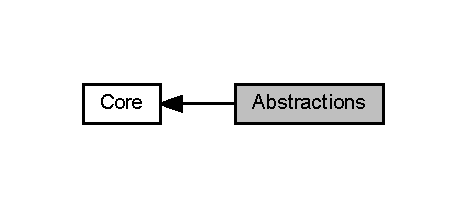
\includegraphics[width=224pt]{group___abstractions}
\end{center}
\end{figure}
\subsection*{Classes}
\begin{DoxyCompactItemize}
\item 
class \hyperlink{class_vision_core_1_1_abstractions_1_1_abstract_auto_tracker}{Abstract\+Auto\+Tracker$<$ T\+Img, T\+Obj $>$}
\begin{DoxyCompactList}\small\item\em Implements a tracker that can automatically detect and track multiple objects by creating a individual tracker for each object. \end{DoxyCompactList}\item 
class \hyperlink{class_vision_core_1_1_abstractions_1_1_detector_based_tracker}{Detector\+Based\+Tracker$<$ T\+Img, T\+Obj $>$}
\begin{DoxyCompactList}\small\item\em A simple tracker that applies a detector on every frame. \end{DoxyCompactList}\item 
class \hyperlink{class_vision_core_1_1_abstractions_1_1_detector_based_multi_tracker}{Detector\+Based\+Multi\+Tracker$<$ T\+Img, T\+Obj $>$}
\begin{DoxyCompactList}\small\item\em A tracker that applies a detector on every frame. \end{DoxyCompactList}\item 
class \hyperlink{class_vision_core_1_1_abstractions_1_1_detector_logger}{Detector\+Logger$<$ T\+Img, T\+Obj $>$}
\begin{DoxyCompactList}\small\item\em Provides log functionalities for a detector. Stores results, processing times and statistics. \end{DoxyCompactList}\item 
class \hyperlink{class_vision_core_1_1_abstractions_1_1_tracker_logger}{Tracker\+Logger$<$ T\+Img, T\+Obj $>$}
\begin{DoxyCompactList}\small\item\em Provides log functionalities for a Tracker. Stores results, processing times and statistics. \end{DoxyCompactList}\item 
class \hyperlink{class_vision_core_1_1_abstractions_1_1_abstract_particle_filtering_tracker}{Abstract\+Particle\+Filtering\+Tracker$<$ T\+Img, T\+Obj $>$}
\begin{DoxyCompactList}\small\item\em Implements a particle filtering algorithm for generic tracking models. \end{DoxyCompactList}\end{DoxyCompactItemize}


\subsection{Detailed Description}
Contains abstract computer vision methods. 

This module contains several classes that provide general methods implementations for computer vision methods and higher level applications, such as particle filtering, detector based tracking, loggers, etc. The classes implemented in this module use template generalization for the image and object types. This way, the methods can be used with images from any source (e.\+g. Open\+Cv, Kinect, stereo cameras, termal cameras, etc). It can support diferent object representation as well (e.\+g. rectangles, contours, specific structs, etc). 
\hypertarget{group___async}{}\section{Async}
\label{group___async}\index{Async@{Async}}


Contains classes that execute the Cv\+Works methods asynchronously in separate threads.  


Collaboration diagram for Async\+:
\nopagebreak
\begin{figure}[H]
\begin{center}
\leavevmode
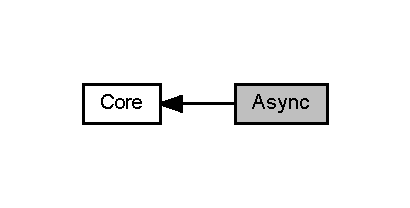
\includegraphics[width=197pt]{group___async}
\end{center}
\end{figure}
\subsection*{Classes}
\begin{DoxyCompactItemize}
\item 
class \hyperlink{class_vision_core_1_1_async_1_1_async_frame_server_wrap}{Async\+Frame\+Server\+Wrap$<$ T\+Img $>$}
\begin{DoxyCompactList}\small\item\em Allows the execution of a frame server asynchronously in an individual thread. \end{DoxyCompactList}\item 
class \hyperlink{class_vision_core_1_1_async_1_1_async_vision_execution}{Async\+Vision\+Execution$<$ T\+Img, T\+Out $>$}
\begin{DoxyCompactList}\small\item\em Allows the execution of a vision method asynchronously in an individual thread. \end{DoxyCompactList}\item 
class \hyperlink{class_vision_core_1_1_async_1_1_async_detector_wrap}{Async\+Detector\+Wrap$<$ T\+Img, T\+Obj $>$}
\begin{DoxyCompactList}\small\item\em Allows the execution of a detector asynchronously in an individual thread. \end{DoxyCompactList}\item 
class \hyperlink{class_vision_core_1_1_async_1_1_async_tracker_wrap}{Async\+Tracker\+Wrap$<$ T\+Img, T\+Obj $>$}
\begin{DoxyCompactList}\small\item\em Allows the execution of a tracker asynchronously in an individual thread. \end{DoxyCompactList}\end{DoxyCompactItemize}


\subsection{Detailed Description}
Contains classes that execute the Cv\+Works methods asynchronously in separate threads. 

The classes in this module work as wraps that receive an object (detector, tracker, etc) and coordinate its execution in individual threads. 
\hypertarget{group___core}{}\section{Core}
\label{group___core}\index{Core@{Core}}


This module combines several sub-\/modules that form the core functionalities of Cv\+Works.  


Collaboration diagram for Core\+:
\nopagebreak
\begin{figure}[H]
\begin{center}
\leavevmode
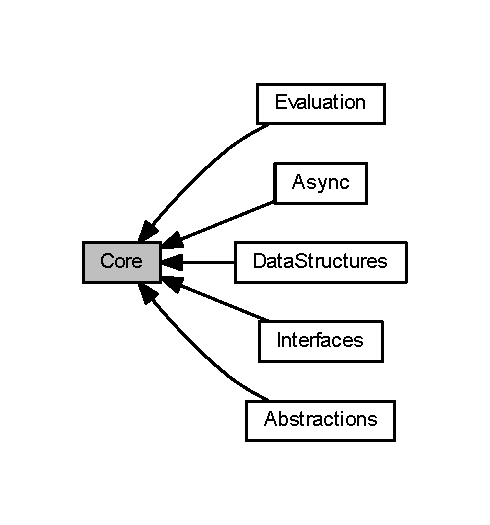
\includegraphics[width=235pt]{group___core}
\end{center}
\end{figure}
\subsection*{Modules}
\begin{DoxyCompactItemize}
\item 
\hyperlink{group___abstractions}{Abstractions}
\begin{DoxyCompactList}\small\item\em Contains abstract computer vision methods. \end{DoxyCompactList}\item 
\hyperlink{group___async}{Async}
\begin{DoxyCompactList}\small\item\em Contains classes that execute the Cv\+Works methods asynchronously in separate threads. \end{DoxyCompactList}\item 
\hyperlink{group___data_structures}{Data\+Structures}
\begin{DoxyCompactList}\small\item\em Declaration and implementation of simple data structures for Vision framework. \end{DoxyCompactList}\item 
\hyperlink{group___evaluation}{Evaluation}
\begin{DoxyCompactList}\small\item\em Implementation of generic validation algorithms for Cv\+Works interfaces. \end{DoxyCompactList}\item 
\hyperlink{group___interfaces}{Interfaces}
\begin{DoxyCompactList}\small\item\em This module contains the generic interfaces used throughout the framework. \end{DoxyCompactList}\end{DoxyCompactItemize}


\subsection{Detailed Description}
This module combines several sub-\/modules that form the core functionalities of Cv\+Works. 

\begin{DoxySeeAlso}{See also}
\hyperlink{group___interfaces}{Interfaces} \hyperlink{group___abstractions}{Abstractions} \hyperlink{group___evaluation}{Evaluation} \hyperlink{group___async}{Async} 
\end{DoxySeeAlso}

\hypertarget{group___data_structures}{}\section{Data\+Structures}
\label{group___data_structures}\index{Data\+Structures@{Data\+Structures}}


Declaration and implementation of simple data structures for Vision framework.  


Collaboration diagram for Data\+Structures\+:
\nopagebreak
\begin{figure}[H]
\begin{center}
\leavevmode
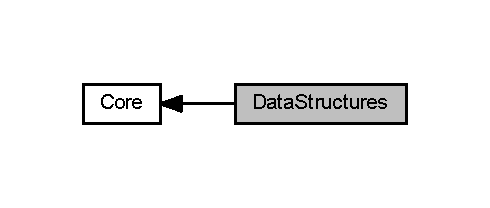
\includegraphics[width=235pt]{group___data_structures}
\end{center}
\end{figure}
Declaration and implementation of simple data structures for Vision framework. 

\begin{DoxySeeAlso}{See also}
\hyperlink{group___interfaces}{Interfaces} \hyperlink{group___abstractions}{Abstractions} \hyperlink{group___evaluation}{Evaluation} \hyperlink{group___async}{Async} 
\end{DoxySeeAlso}

\hypertarget{group___evaluation}{}\section{Evaluation}
\label{group___evaluation}\index{Evaluation@{Evaluation}}


Implementation of generic validation algorithms for Cv\+Works interfaces.  


Collaboration diagram for Evaluation\+:
\nopagebreak
\begin{figure}[H]
\begin{center}
\leavevmode
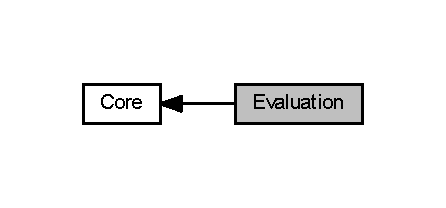
\includegraphics[width=214pt]{group___evaluation}
\end{center}
\end{figure}
\subsection*{Classes}
\begin{DoxyCompactItemize}
\item 
class \hyperlink{class_vision_core_1_1_evaluation_1_1_detection_dataset}{Detection\+Dataset$<$ T\+Img, T\+Obj $>$}
\begin{DoxyCompactList}\small\item\em Abstract class for a generic detection dataset, contining images and its ground-\/truth. \end{DoxyCompactList}\item 
class \hyperlink{class_vision_core_1_1_evaluation_1_1_detection_sub_dataset}{Detection\+Sub\+Dataset$<$ T\+Img, T\+Obj $>$}
\begin{DoxyCompactList}\small\item\em Class that provides access to a subset of a detection dataset. \end{DoxyCompactList}\item 
class \hyperlink{class_vision_core_1_1_evaluation_1_1_tracking_dataset}{Tracking\+Dataset$<$ T\+Img, T\+Obj $>$}
\begin{DoxyCompactList}\small\item\em Abstract class for a generic tracking dataset, containing videos and its ground-\/truth data. \end{DoxyCompactList}\item 
struct \hyperlink{struct_vision_core_1_1_evaluation_1_1_detector_eval_result}{Detector\+Eval\+Result}
\begin{DoxyCompactList}\small\item\em Data structure that stores the statistics and evaluation results for a detector. \end{DoxyCompactList}\item 
class \hyperlink{class_vision_core_1_1_evaluation_1_1_detector_evaluator}{Detector\+Evaluator$<$ T\+Img, T\+Obj1, T\+Obj2 $>$}
\begin{DoxyCompactList}\small\item\em Provides algorithms for performance evaluation of detectors. \end{DoxyCompactList}\item 
struct \hyperlink{struct_vision_core_1_1_evaluation_1_1_binary_classifier_eval_result}{Binary\+Classifier\+Eval\+Result}
\begin{DoxyCompactList}\small\item\em Data structure that stores the statistics and evaluation data for a binary classifier. \end{DoxyCompactList}\item 
struct \hyperlink{struct_vision_core_1_1_evaluation_1_1_tracking_eval_result}{Tracking\+Eval\+Result}
\begin{DoxyCompactList}\small\item\em Data structure that stores the statistics and evaluation results for a tracker. \end{DoxyCompactList}\item 
class \hyperlink{class_vision_core_1_1_evaluation_1_1_tracker_evaluator}{Tracker\+Evaluator$<$ T\+Img, T\+Obj1, T\+Obj2 $>$}
\begin{DoxyCompactList}\small\item\em Provides algorithms for performance evaluation of trackers. \end{DoxyCompactList}\item 
class \hyperlink{class_vision_core_1_1_evaluation_1_1_frame_server_det_data}{Frame\+Server\+Det\+Data$<$ T\+Img, T\+Obj $>$}
\begin{DoxyCompactList}\small\item\em Frame\+Server from a detection dataset. \end{DoxyCompactList}\end{DoxyCompactItemize}


\subsection{Detailed Description}
Implementation of generic validation algorithms for Cv\+Works interfaces. 

In order to use this evaluation methods you need a detector (or tracker) and a set of samples with the ground truth. 
\hypertarget{group___interfaces}{}\section{Interfaces}
\label{group___interfaces}\index{Interfaces@{Interfaces}}


This module contains the generic interfaces used throughout the framework.  


Collaboration diagram for Interfaces\+:
\nopagebreak
\begin{figure}[H]
\begin{center}
\leavevmode
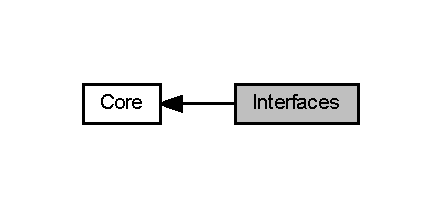
\includegraphics[width=212pt]{group___interfaces}
\end{center}
\end{figure}
\subsection*{Classes}
\begin{DoxyCompactItemize}
\item 
class \hyperlink{class_vision_core_1_1_abstractions_1_1_vision_helpper}{Vision\+Helpper}
\begin{DoxyCompactList}\small\item\em This class defines some generic helper functions that can be overrided to provide key functionalities. \end{DoxyCompactList}\item 
class \hyperlink{class_vision_core_1_1_interfaces_1_1_frame_server}{Frame\+Server$<$ T\+Img $>$}
\begin{DoxyCompactList}\small\item\em Interface for a source of frames. The frames can come from a video file, webcam, set of images, etc. \end{DoxyCompactList}\item 
class \hyperlink{class_vision_core_1_1_interfaces_1_1_detector}{Detector$<$ T\+Img, T\+Obj $>$}
\begin{DoxyCompactList}\small\item\em Interface defining a generic object detector (e.\+g. faces, car, people). \end{DoxyCompactList}\item 
class \hyperlink{class_vision_core_1_1_interfaces_1_1_tracker}{Tracker$<$ T\+Img, T\+Obj $>$}
\begin{DoxyCompactList}\small\item\em Interface defining a generic object tracker. \end{DoxyCompactList}\item 
class \hyperlink{class_vision_core_1_1_interfaces_1_1_identified_multi_tracker}{Identified\+Multi\+Tracker$<$ T\+Img, T\+Obj $>$}
\begin{DoxyCompactList}\small\item\em A \hyperlink{class_vision_core_1_1_interfaces_1_1_identified_multi_tracker}{Identified\+Multi\+Tracker} is a tracker for multiple objects, each having its own I\+D. \end{DoxyCompactList}\item 
class \hyperlink{class_vision_core_1_1_interfaces_1_1_categorizer}{Categorizer$<$ T\+In, T\+Ctg $>$}
\begin{DoxyCompactList}\small\item\em Interface defining a generic image categorizer (classifier). \end{DoxyCompactList}\end{DoxyCompactItemize}


\subsection{Detailed Description}
This module contains the generic interfaces used throughout the framework. 

The objective of these interfaces is to define minimal functionalities that detectors, trackers, categorizers, etc should implement.

The image type and object is generalized by using templates, so these interfaces can be implemented for different types of images (e.\+g. Open\+Cv, Kinect, stereo cameras, C\+P\+L cloud points, etc) and for different types of objects (e.\+g. faces, cars, gestures, etc). 
\hypertarget{group___viscv}{}\section{Viscv}
\label{group___viscv}\index{Viscv@{Viscv}}


This component groups some detectors and trackers based on Open\+Cv.  


\subsection*{Classes}
\begin{DoxyCompactItemize}
\item 
class \hyperlink{class_viscv_1_1_a_r_tag_detector_b_l_p}{A\+R\+Tag\+Detector\+B\+L\+P}
\begin{DoxyCompactList}\small\item\em Implements a augmented reality tag detector. \end{DoxyCompactList}\item 
class \hyperlink{class_viscv_1_1_circle_detector_h_t_c_f}{Circle\+Detector\+H\+T\+C\+F}
\begin{DoxyCompactList}\small\item\em Detects circles using Hough Transform and (optionally) Color Filter (H\+T\+C\+F). \end{DoxyCompactList}\item 
class \hyperlink{class_viscv_1_1_circle_tracker_h_t_c_f}{Circle\+Tracker\+H\+T\+C\+F}
\begin{DoxyCompactList}\small\item\em Rastreador baseado na classe \hyperlink{class_viscv_1_1_circle_detector_h_t_c_f}{Circle\+Detector\+H\+T\+C\+F}. \end{DoxyCompactList}\item 
class \hyperlink{class_viscv_1_1_color_blob_detector_h_f}{Color\+Blob\+Detector\+H\+F}
\begin{DoxyCompactList}\small\item\em Implementa um detector de blobs baseado em cor. \end{DoxyCompactList}\item 
class \hyperlink{class_viscv_1_1_cv_image_g_u_i}{Cv\+Image\+G\+U\+I}
\begin{DoxyCompactList}\small\item\em Esta classe cria uma janela para exibição de imagens. \end{DoxyCompactList}\item 
class \hyperlink{class_viscv_1_1_dataset_f_d_d_b}{Dataset\+F\+D\+D\+B}
\begin{DoxyCompactList}\small\item\em Dataset público de várias imagens contendo pessoas em ambientes do dia-\/a-\/dia. \end{DoxyCompactList}\item 
class \hyperlink{class_viscv_1_1_feature_tracker_k_l_t_cv}{Feature\+Tracker\+K\+L\+T\+Cv}
\begin{DoxyCompactList}\small\item\em Kanade-\/\+Lucas Tracker using Open\+Cv implementation. \end{DoxyCompactList}\item 
class \hyperlink{class_viscv_1_1_frame_server_cv}{Frame\+Server\+Cv}
\begin{DoxyCompactList}\small\item\em Implementantion of interface Frame\+Server using Open\+Cv. \end{DoxyCompactList}\item 
class \hyperlink{class_viscv_1_1_line_detector_h_t}{Line\+Detector\+H\+T}
\begin{DoxyCompactList}\small\item\em Detector de linhas simples. \end{DoxyCompactList}\item 
class \hyperlink{class_viscv_1_1_multi_object_tracker_c_c_cv}{Multi\+Object\+Tracker\+C\+C\+Cv}
\begin{DoxyCompactList}\small\item\em Detecta e rastreia multiplos objetos utilizando o rastreador \textquotesingle{}\hyperlink{class_viscv_1_1_object_tracker_c_c_cv}{Object\+Tracker\+C\+C\+Cv}\textquotesingle{}. \end{DoxyCompactList}\item 
class \hyperlink{class_viscv_1_1_object_detector_c_c_cv}{Object\+Detector\+C\+C\+Cv}
\begin{DoxyCompactList}\small\item\em A wrapper to Open\+Cv haar detector. \end{DoxyCompactList}\item 
class \hyperlink{class_viscv_1_1_object_detector_f_m_cv}{Object\+Detector\+F\+M\+Cv}
\begin{DoxyCompactList}\small\item\em Implementa um detector de objetos genéricos utilizando S\+I\+F\+T features. \end{DoxyCompactList}\item 
class \hyperlink{class_viscv_1_1_object_tracker_c_c_cv}{Object\+Tracker\+C\+C\+Cv}
\begin{DoxyCompactList}\small\item\em Simple tracker using Open\+Cv cascade classifier detector. \end{DoxyCompactList}\item 
class \hyperlink{class_viscv_1_1_object_tracker_k_l_t}{Object\+Tracker\+K\+L\+T}
\begin{DoxyCompactList}\small\item\em Usa o método Kanade-\/\+Lucas de rastreamento de pontos para rastrear um objeto. \end{DoxyCompactList}\item 
class \hyperlink{class_viscv_1_1_object_tracker_p_f_hist}{Object\+Tracker\+P\+F\+Hist}
\begin{DoxyCompactList}\small\item\em Particle Filtering with histogram matching. \end{DoxyCompactList}\item 
class \hyperlink{class_viscv_1_1_templ_matching_detector}{Templ\+Matching\+Detector}
\begin{DoxyCompactList}\small\item\em Detecta objetos usando template matching. \end{DoxyCompactList}\item 
class \hyperlink{class_viscv_1_1_templ_matching_tracker}{Templ\+Matching\+Tracker}
\begin{DoxyCompactList}\small\item\em Rastreia objetos usando template matching. \end{DoxyCompactList}\end{DoxyCompactItemize}


\subsection{Detailed Description}
This component groups some detectors and trackers based on Open\+Cv. 

This component provides some detection and tracking methods (such as Haar Cascade Classifier detectors, Lucas-\/\+Kanade tracker, S\+I\+F\+T based detection, etc) based on Open\+Cv library. The methods can be usefull in applications, as well as serve as examples on how to implement Cv\+Works interfaces.

\begin{DoxySeeAlso}{See also}
\hyperlink{_vision_implementation_cv_8h_source}{Vision\+Implementation\+Cv.\+h} 
\end{DoxySeeAlso}

\hypertarget{group___vision_g_u_i}{}\section{Vision\+G\+U\+I}
\label{group___vision_g_u_i}\index{Vision\+G\+U\+I@{Vision\+G\+U\+I}}


Aplicativo que apresenta uma interface gráfica de usuário (G\+U\+I) para demonstração dos métodos do Framework.  


\subsection*{Classes}
\begin{DoxyCompactItemize}
\item 
class \hyperlink{class_detector_control}{Detector\+Control$<$ T\+Img, T\+Obj $>$}
\begin{DoxyCompactList}\small\item\em Esta classe é responsável por controlar a execução de um detector. \end{DoxyCompactList}\item 
class \hyperlink{class_frame_server_control_widget}{Frame\+Server\+Control\+Widget}
\begin{DoxyCompactList}\small\item\em Esta classe controla a execução e representação gráfica de um vídeo (Frame\+Server). \end{DoxyCompactList}\item 
class \hyperlink{class_image_viewer_cv}{Image\+Viewer\+Cv}
\begin{DoxyCompactList}\small\item\em Esta classe implementa um widget capaz de mostrar uma imagem do tipo cv\+::\+Mat. \end{DoxyCompactList}\item 
class \hyperlink{class_process_control}{Process\+Control}
\begin{DoxyCompactList}\small\item\em Esta classe é responsável por controlar a execuçãoo de um algoritmo de visão computacional. \end{DoxyCompactList}\item 
class \hyperlink{class_process_widget}{Process\+Widget}
\begin{DoxyCompactList}\small\item\em Interface gráfica para um objeto \hyperlink{class_process_control}{Process\+Control}. Mostra funcionalidades básicas de controle (fechar, pausar, definir cor de desenho). \end{DoxyCompactList}\item 
class \hyperlink{class_tracker_control}{Tracker\+Control$<$ T\+Img, T\+Obj $>$}
\begin{DoxyCompactList}\small\item\em Esta classe é responsável por controlar a execução de um rastreador. \end{DoxyCompactList}\item 
class \hyperlink{class_face_detector_control}{Face\+Detector\+Control}
\begin{DoxyCompactList}\small\item\em Esta classe é responsável por controlar a execução de um detector de objetos do tipo Object\+Detector\+C\+C\+Cv. \end{DoxyCompactList}\item 
class \hyperlink{class_feature_tracker_control}{Feature\+Tracker\+Control}
\begin{DoxyCompactList}\small\item\em Esta classe é responsável por controlar a execução de um rastreador do tipo Feature\+Tracker\+K\+L\+T\+Cv. \end{DoxyCompactList}\item 
class \hyperlink{class_main_window}{Main\+Window}
\begin{DoxyCompactList}\small\item\em Classe principal da G\+U\+I. \end{DoxyCompactList}\item 
class \hyperlink{class_object_tracker_p_f_hist_control}{Object\+Tracker\+P\+F\+Hist\+Control}
\begin{DoxyCompactList}\small\item\em Esta classe é responsável por controlar a execução de um rastreador do tipo Object\+Tracker\+P\+F\+Hist. \end{DoxyCompactList}\end{DoxyCompactItemize}


\subsection{Detailed Description}
Aplicativo que apresenta uma interface gráfica de usuário (G\+U\+I) para demonstração dos métodos do Framework. 


\chapter{Namespace Documentation}
\hypertarget{namespace_viscv}{}\section{Viscv Namespace Reference}
\label{namespace_viscv}\index{Viscv@{Viscv}}


Provides several computer vision methods for detection an.  


\subsection*{Classes}
\begin{DoxyCompactItemize}
\item 
class \hyperlink{class_viscv_1_1_a_r_tag}{A\+R\+Tag}
\begin{DoxyCompactList}\small\item\em Defines a augmented reality tag, which contains a bounding polygon and a tag I\+D. \end{DoxyCompactList}\item 
class \hyperlink{class_viscv_1_1_a_r_tag_detector_b_l_p}{A\+R\+Tag\+Detector\+B\+L\+P}
\begin{DoxyCompactList}\small\item\em Implements a augmented reality tag detector. \end{DoxyCompactList}\item 
class \hyperlink{class_viscv_1_1_circle}{Circle}
\begin{DoxyCompactList}\small\item\em Defines a circle. Stores the center (x,y) and radius. \end{DoxyCompactList}\item 
class \hyperlink{class_viscv_1_1_circle_detector_h_t_c_f}{Circle\+Detector\+H\+T\+C\+F}
\begin{DoxyCompactList}\small\item\em Detects circles using Hough Transform and (optionally) Color Filter (H\+T\+C\+F). \end{DoxyCompactList}\item 
class \hyperlink{class_viscv_1_1_circle_tracker_h_t_c_f}{Circle\+Tracker\+H\+T\+C\+F}
\begin{DoxyCompactList}\small\item\em Rastreador baseado na classe \hyperlink{class_viscv_1_1_circle_detector_h_t_c_f}{Circle\+Detector\+H\+T\+C\+F}. \end{DoxyCompactList}\item 
class \hyperlink{class_viscv_1_1_color_blob_detector_h_f}{Color\+Blob\+Detector\+H\+F}
\begin{DoxyCompactList}\small\item\em Implementa um detector de blobs baseado em cor. \end{DoxyCompactList}\item 
class \hyperlink{class_viscv_1_1_cv_image_g_u_i}{Cv\+Image\+G\+U\+I}
\begin{DoxyCompactList}\small\item\em Esta classe cria uma janela para exibição de imagens. \end{DoxyCompactList}\item 
class \hyperlink{class_viscv_1_1_dataset_f_d_d_b}{Dataset\+F\+D\+D\+B}
\begin{DoxyCompactList}\small\item\em Dataset público de várias imagens contendo pessoas em ambientes do dia-\/a-\/dia. \end{DoxyCompactList}\item 
class \hyperlink{class_viscv_1_1_feature_tracker_k_l_t_cv}{Feature\+Tracker\+K\+L\+T\+Cv}
\begin{DoxyCompactList}\small\item\em Kanade-\/\+Lucas Tracker using Open\+Cv implementation. \end{DoxyCompactList}\item 
class \hyperlink{class_viscv_1_1_frame_server_cv}{Frame\+Server\+Cv}
\begin{DoxyCompactList}\small\item\em Implementantion of interface Frame\+Server using Open\+Cv. \end{DoxyCompactList}\item 
class \hyperlink{class_viscv_1_1_line}{Line}
\item 
class \hyperlink{class_viscv_1_1_line_detector_h_t}{Line\+Detector\+H\+T}
\begin{DoxyCompactList}\small\item\em Detector de linhas simples. \end{DoxyCompactList}\item 
class \hyperlink{class_viscv_1_1_multi_object_tracker_c_c_cv}{Multi\+Object\+Tracker\+C\+C\+Cv}
\begin{DoxyCompactList}\small\item\em Detecta e rastreia multiplos objetos utilizando o rastreador \textquotesingle{}\hyperlink{class_viscv_1_1_object_tracker_c_c_cv}{Object\+Tracker\+C\+C\+Cv}\textquotesingle{}. \end{DoxyCompactList}\item 
class \hyperlink{class_viscv_1_1_object_detector_c_c_cv}{Object\+Detector\+C\+C\+Cv}
\begin{DoxyCompactList}\small\item\em A wrapper to Open\+Cv haar detector. \end{DoxyCompactList}\item 
class \hyperlink{class_viscv_1_1_object_detector_f_m_cv}{Object\+Detector\+F\+M\+Cv}
\begin{DoxyCompactList}\small\item\em Implementa um detector de objetos genéricos utilizando S\+I\+F\+T features. \end{DoxyCompactList}\item 
class \hyperlink{class_viscv_1_1_object_tracker_c_c_cv}{Object\+Tracker\+C\+C\+Cv}
\begin{DoxyCompactList}\small\item\em Simple tracker using Open\+Cv cascade classifier detector. \end{DoxyCompactList}\item 
class \hyperlink{class_viscv_1_1_object_tracker_k_l_t}{Object\+Tracker\+K\+L\+T}
\begin{DoxyCompactList}\small\item\em Usa o método Kanade-\/\+Lucas de rastreamento de pontos para rastrear um objeto. \end{DoxyCompactList}\item 
class \hyperlink{class_viscv_1_1_object_tracker_p_f_hist}{Object\+Tracker\+P\+F\+Hist}
\begin{DoxyCompactList}\small\item\em Particle Filtering with histogram matching. \end{DoxyCompactList}\item 
class \hyperlink{class_viscv_1_1_polygon}{Polygon}
\begin{DoxyCompactList}\small\item\em Defines a generic polygon with fixed number of vertices. \end{DoxyCompactList}\item 
class \hyperlink{class_viscv_1_1_templ_matching_detector}{Templ\+Matching\+Detector}
\begin{DoxyCompactList}\small\item\em Detecta objetos usando template matching. \end{DoxyCompactList}\item 
class \hyperlink{class_viscv_1_1_templ_matching_tracker}{Templ\+Matching\+Tracker}
\begin{DoxyCompactList}\small\item\em Rastreia objetos usando template matching. \end{DoxyCompactList}\end{DoxyCompactItemize}


\subsection{Detailed Description}
Provides several computer vision methods for detection an. 
\hypertarget{namespace_vision_core}{}\section{Vision\+Core Namespace Reference}
\label{namespace_vision_core}\index{Vision\+Core@{Vision\+Core}}


Contains the core functionalities of Cv\+Works.  


\subsection*{Namespaces}
\begin{DoxyCompactItemize}
\item 
 \hyperlink{namespace_vision_core_1_1_abstractions}{Abstractions}
\begin{DoxyCompactList}\small\item\em Generic computer vision methods and functionalities. \end{DoxyCompactList}\item 
 \hyperlink{namespace_vision_core_1_1_async}{Async}
\begin{DoxyCompactList}\small\item\em Provides classes for running computer vision tasks in multiple threads. \end{DoxyCompactList}\item 
 \hyperlink{namespace_vision_core_1_1_data_structures}{Data\+Structures}
\begin{DoxyCompactList}\small\item\em Data structures used within Cv\+Works. \end{DoxyCompactList}\item 
 \hyperlink{namespace_vision_core_1_1_evaluation}{Evaluation}
\begin{DoxyCompactList}\small\item\em \hyperlink{namespace_vision_core_1_1_evaluation}{Evaluation} methods for computer vision tasks. \end{DoxyCompactList}\item 
 \hyperlink{namespace_vision_core_1_1_interfaces}{Interfaces}
\begin{DoxyCompactList}\small\item\em \hyperlink{namespace_vision_core_1_1_interfaces}{Interfaces} for generic computer vision tasks. \end{DoxyCompactList}\end{DoxyCompactItemize}


\subsection{Detailed Description}
Contains the core functionalities of Cv\+Works. 

The core functionalities should be independent of image representation. It should be implemented as a header only library and should not depend on external libraries. 
\hypertarget{namespace_vision_core_1_1_abstractions}{}\section{Vision\+Core\+:\+:Abstractions Namespace Reference}
\label{namespace_vision_core_1_1_abstractions}\index{Vision\+Core\+::\+Abstractions@{Vision\+Core\+::\+Abstractions}}


Generic computer vision methods and functionalities.  


\subsection*{Classes}
\begin{DoxyCompactItemize}
\item 
class \hyperlink{class_vision_core_1_1_abstractions_1_1_abstract_auto_tracker}{Abstract\+Auto\+Tracker}
\begin{DoxyCompactList}\small\item\em Implements a tracker that can automatically detect and track multiple objects by creating a individual tracker for each object. \end{DoxyCompactList}\item 
class \hyperlink{class_vision_core_1_1_abstractions_1_1_abstract_particle_filtering_tracker}{Abstract\+Particle\+Filtering\+Tracker}
\begin{DoxyCompactList}\small\item\em Implements a particle filtering algorithm for generic tracking models. \end{DoxyCompactList}\item 
struct \hyperlink{struct_vision_core_1_1_abstractions_1_1_detection_data}{Detection\+Data}
\begin{DoxyCompactList}\small\item\em Simple structure that stores data related to a detection (used in Detection\+Logger). \end{DoxyCompactList}\item 
class \hyperlink{class_vision_core_1_1_abstractions_1_1_detector_based_multi_tracker}{Detector\+Based\+Multi\+Tracker}
\begin{DoxyCompactList}\small\item\em A tracker that applies a detector on every frame. \end{DoxyCompactList}\item 
class \hyperlink{class_vision_core_1_1_abstractions_1_1_detector_based_tracker}{Detector\+Based\+Tracker}
\begin{DoxyCompactList}\small\item\em A simple tracker that applies a detector on every frame. \end{DoxyCompactList}\item 
class \hyperlink{class_vision_core_1_1_abstractions_1_1_detector_logger}{Detector\+Logger}
\begin{DoxyCompactList}\small\item\em Provides log functionalities for a detector. Stores results, processing times and statistics. \end{DoxyCompactList}\item 
class \hyperlink{class_vision_core_1_1_abstractions_1_1_tracker_logger}{Tracker\+Logger}
\begin{DoxyCompactList}\small\item\em Provides log functionalities for a Tracker. Stores results, processing times and statistics. \end{DoxyCompactList}\item 
struct \hyperlink{struct_vision_core_1_1_abstractions_1_1_tracking_data}{Tracking\+Data}
\begin{DoxyCompactList}\small\item\em Simple structure that stores data related to tracking. Used in \hyperlink{class_vision_core_1_1_abstractions_1_1_tracker_logger}{Tracker\+Logger}. \end{DoxyCompactList}\item 
class \hyperlink{class_vision_core_1_1_abstractions_1_1_vision_helpper}{Vision\+Helpper}
\begin{DoxyCompactList}\small\item\em This class defines some generic helper functions that can be overrided to provide key functionalities. \end{DoxyCompactList}\end{DoxyCompactItemize}


\subsection{Detailed Description}
Generic computer vision methods and functionalities. 
\hypertarget{namespace_vision_core_1_1_async}{}\section{Vision\+Core\+:\+:Async Namespace Reference}
\label{namespace_vision_core_1_1_async}\index{Vision\+Core\+::\+Async@{Vision\+Core\+::\+Async}}


Provides classes for running computer vision tasks in multiple threads.  


\subsection*{Classes}
\begin{DoxyCompactItemize}
\item 
class \hyperlink{class_vision_core_1_1_async_1_1_async_detector_wrap}{Async\+Detector\+Wrap}
\begin{DoxyCompactList}\small\item\em Allows the execution of a detector asynchronously in an individual thread. \end{DoxyCompactList}\item 
class \hyperlink{class_vision_core_1_1_async_1_1_async_frame_server_wrap}{Async\+Frame\+Server\+Wrap}
\begin{DoxyCompactList}\small\item\em Allows the execution of a frame server asynchronously in an individual thread. \end{DoxyCompactList}\item 
class \hyperlink{class_vision_core_1_1_async_1_1_async_tracker_wrap}{Async\+Tracker\+Wrap}
\begin{DoxyCompactList}\small\item\em Allows the execution of a tracker asynchronously in an individual thread. \end{DoxyCompactList}\item 
class \hyperlink{class_vision_core_1_1_async_1_1_async_vision_execution}{Async\+Vision\+Execution}
\begin{DoxyCompactList}\small\item\em Allows the execution of a vision method asynchronously in an individual thread. \end{DoxyCompactList}\end{DoxyCompactItemize}


\subsection{Detailed Description}
Provides classes for running computer vision tasks in multiple threads. 
\hypertarget{namespace_vision_core_1_1_data_structures}{}\section{Vision\+Core\+:\+:Data\+Structures Namespace Reference}
\label{namespace_vision_core_1_1_data_structures}\index{Vision\+Core\+::\+Data\+Structures@{Vision\+Core\+::\+Data\+Structures}}


Data structures used within Cv\+Works.  


\subsection*{Classes}
\begin{DoxyCompactItemize}
\item 
struct \hyperlink{struct_vision_core_1_1_data_structures_1_1_frame}{Frame}
\begin{DoxyCompactList}\small\item\em A \hyperlink{struct_vision_core_1_1_data_structures_1_1_frame}{Frame} contains an image, number and timestamp from a video sequence. \end{DoxyCompactList}\end{DoxyCompactItemize}


\subsection{Detailed Description}
Data structures used within Cv\+Works. 
\hypertarget{namespace_vision_core_1_1_evaluation}{}\section{Vision\+Core\+:\+:Evaluation Namespace Reference}
\label{namespace_vision_core_1_1_evaluation}\index{Vision\+Core\+::\+Evaluation@{Vision\+Core\+::\+Evaluation}}


\hyperlink{namespace_vision_core_1_1_evaluation}{Evaluation} methods for computer vision tasks.  


\subsection*{Classes}
\begin{DoxyCompactItemize}
\item 
struct \hyperlink{struct_vision_core_1_1_evaluation_1_1_binary_classifier_eval_result}{Binary\+Classifier\+Eval\+Result}
\begin{DoxyCompactList}\small\item\em Data structure that stores the statistics and evaluation data for a binary classifier. \end{DoxyCompactList}\item 
class \hyperlink{class_vision_core_1_1_evaluation_1_1_binary_classifier_evaluator}{Binary\+Classifier\+Evaluator}
\item 
class \hyperlink{class_vision_core_1_1_evaluation_1_1_detection_dataset}{Detection\+Dataset}
\begin{DoxyCompactList}\small\item\em Abstract class for a generic detection dataset, contining images and its ground-\/truth. \end{DoxyCompactList}\item 
class \hyperlink{class_vision_core_1_1_evaluation_1_1_detection_sub_dataset}{Detection\+Sub\+Dataset}
\begin{DoxyCompactList}\small\item\em Class that provides access to a subset of a detection dataset. \end{DoxyCompactList}\item 
struct \hyperlink{struct_vision_core_1_1_evaluation_1_1_detector_eval_result}{Detector\+Eval\+Result}
\begin{DoxyCompactList}\small\item\em Data structure that stores the statistics and evaluation results for a detector. \end{DoxyCompactList}\item 
class \hyperlink{class_vision_core_1_1_evaluation_1_1_detector_evaluator}{Detector\+Evaluator}
\begin{DoxyCompactList}\small\item\em Provides algorithms for performance evaluation of detectors. \end{DoxyCompactList}\item 
class \hyperlink{class_vision_core_1_1_evaluation_1_1_frame_server_det_data}{Frame\+Server\+Det\+Data}
\begin{DoxyCompactList}\small\item\em Frame\+Server from a detection dataset. \end{DoxyCompactList}\item 
class \hyperlink{class_vision_core_1_1_evaluation_1_1_tracker_evaluator}{Tracker\+Evaluator}
\begin{DoxyCompactList}\small\item\em Provides algorithms for performance evaluation of trackers. \end{DoxyCompactList}\item 
class \hyperlink{class_vision_core_1_1_evaluation_1_1_tracking_dataset}{Tracking\+Dataset}
\begin{DoxyCompactList}\small\item\em Abstract class for a generic tracking dataset, containing videos and its ground-\/truth data. \end{DoxyCompactList}\item 
struct \hyperlink{struct_vision_core_1_1_evaluation_1_1_tracking_eval_result}{Tracking\+Eval\+Result}
\begin{DoxyCompactList}\small\item\em Data structure that stores the statistics and evaluation results for a tracker. \end{DoxyCompactList}\end{DoxyCompactItemize}


\subsection{Detailed Description}
\hyperlink{namespace_vision_core_1_1_evaluation}{Evaluation} methods for computer vision tasks. 
\hypertarget{namespace_vision_core_1_1_interfaces}{}\section{Vision\+Core\+:\+:Interfaces Namespace Reference}
\label{namespace_vision_core_1_1_interfaces}\index{Vision\+Core\+::\+Interfaces@{Vision\+Core\+::\+Interfaces}}


\hyperlink{namespace_vision_core_1_1_interfaces}{Interfaces} for generic computer vision tasks.  


\subsection*{Classes}
\begin{DoxyCompactItemize}
\item 
class \hyperlink{class_vision_core_1_1_interfaces_1_1_categorizer}{Categorizer}
\begin{DoxyCompactList}\small\item\em Interface defining a generic image categorizer (classifier). \end{DoxyCompactList}\item 
class \hyperlink{class_vision_core_1_1_interfaces_1_1_detector}{Detector}
\begin{DoxyCompactList}\small\item\em Interface defining a generic object detector (e.\+g. faces, car, people). \end{DoxyCompactList}\item 
class \hyperlink{class_vision_core_1_1_interfaces_1_1_frame_server}{Frame\+Server}
\begin{DoxyCompactList}\small\item\em Interface for a source of frames. The frames can come from a video file, webcam, set of images, etc. \end{DoxyCompactList}\item 
class \hyperlink{class_vision_core_1_1_interfaces_1_1_identified_multi_tracker}{Identified\+Multi\+Tracker}
\begin{DoxyCompactList}\small\item\em A \hyperlink{class_vision_core_1_1_interfaces_1_1_identified_multi_tracker}{Identified\+Multi\+Tracker} is a tracker for multiple objects, each having its own I\+D. \end{DoxyCompactList}\item 
class \hyperlink{class_vision_core_1_1_interfaces_1_1_tracker}{Tracker}
\begin{DoxyCompactList}\small\item\em Interface defining a generic object tracker. \end{DoxyCompactList}\end{DoxyCompactItemize}


\subsection{Detailed Description}
\hyperlink{namespace_vision_core_1_1_interfaces}{Interfaces} for generic computer vision tasks. 
\chapter{Class Documentation}
\hypertarget{class_vision_core_1_1_abstractions_1_1_abstract_auto_tracker}{}\section{Abstract\+Auto\+Tracker$<$ T\+Img, T\+Obj $>$ Class Template Reference}
\label{class_vision_core_1_1_abstractions_1_1_abstract_auto_tracker}\index{Abstract\+Auto\+Tracker$<$ T\+Img, T\+Obj $>$@{Abstract\+Auto\+Tracker$<$ T\+Img, T\+Obj $>$}}


Implements a tracker that can automatically detect and track multiple objects by creating a individual tracker for each object.  




{\ttfamily \#include $<$Vision\+Abstractions.\+h$>$}



Inheritance diagram for Abstract\+Auto\+Tracker$<$ T\+Img, T\+Obj $>$\+:
\nopagebreak
\begin{figure}[H]
\begin{center}
\leavevmode
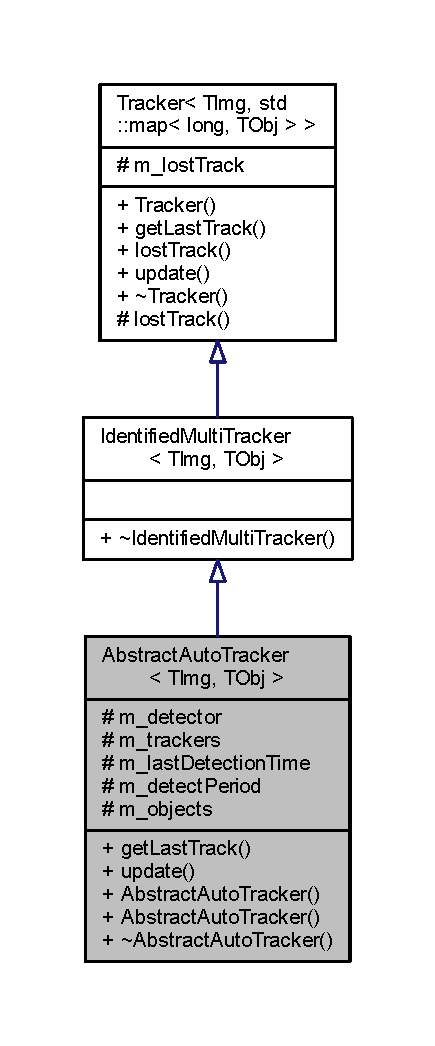
\includegraphics[width=209pt]{class_vision_core_1_1_abstractions_1_1_abstract_auto_tracker__inherit__graph}
\end{center}
\end{figure}


Collaboration diagram for Abstract\+Auto\+Tracker$<$ T\+Img, T\+Obj $>$\+:
\nopagebreak
\begin{figure}[H]
\begin{center}
\leavevmode
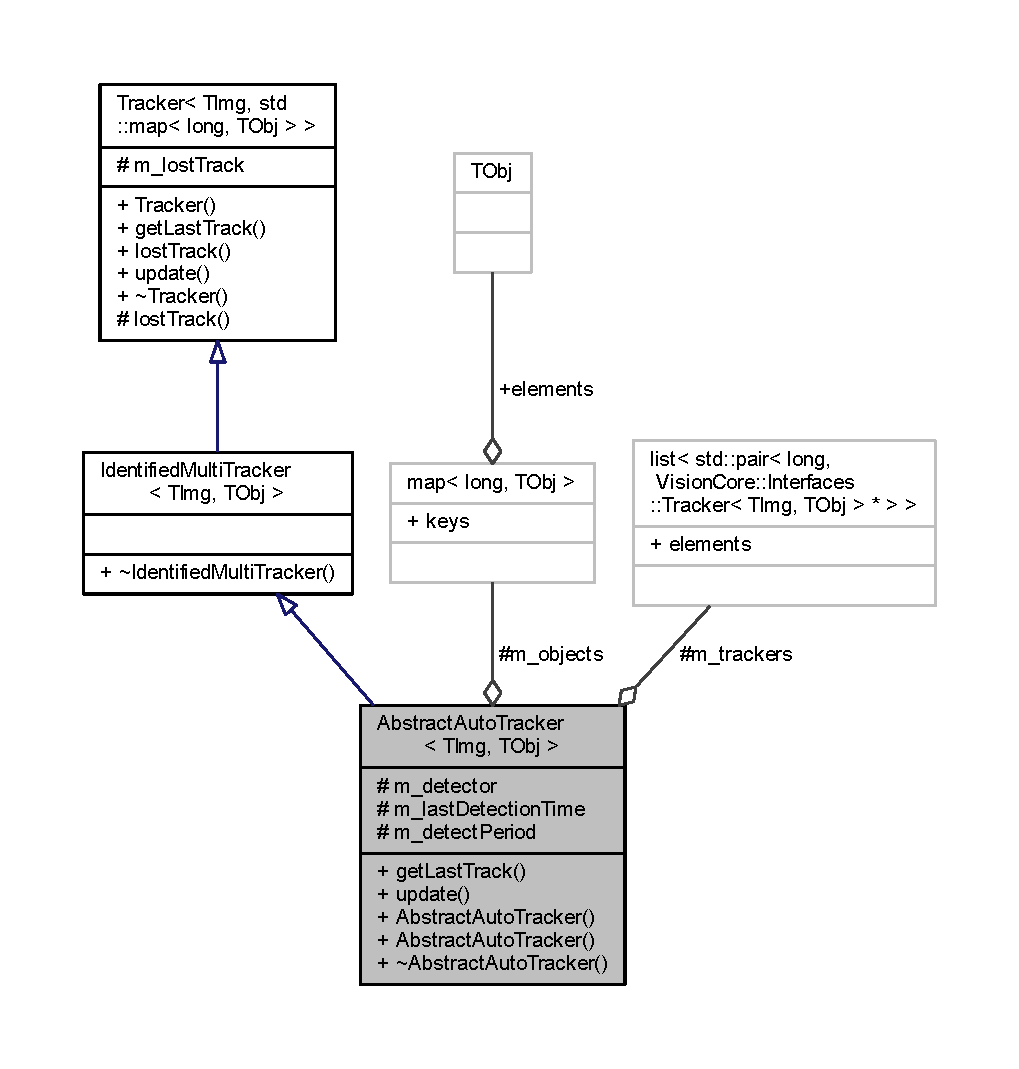
\includegraphics[width=350pt]{class_vision_core_1_1_abstractions_1_1_abstract_auto_tracker__coll__graph}
\end{center}
\end{figure}
\subsection*{Public Member Functions}
\begin{DoxyCompactItemize}
\item 
virtual const std\+::map$<$ long, T\+Obj $>$ \& \hyperlink{class_vision_core_1_1_abstractions_1_1_abstract_auto_tracker_afdfc24d8a5f14f873caf5e1d3ff55546}{get\+Last\+Track} ()
\begin{DoxyCompactList}\small\item\em Returns a reference to the current estimated object state. \end{DoxyCompactList}\item 
virtual void \hyperlink{class_vision_core_1_1_abstractions_1_1_abstract_auto_tracker_af1a54610c9af7fb54d00e4be2e75609e}{update} (const \hyperlink{struct_vision_core_1_1_data_structures_1_1_frame}{Frame}$<$ T\+Img $>$ \&frame)
\begin{DoxyCompactList}\small\item\em Updates the object position (state) given a new frame. \end{DoxyCompactList}\item 
\hypertarget{class_vision_core_1_1_abstractions_1_1_abstract_auto_tracker_a03660bad671c2ebfd95f6aa1ce28c052}{}\hyperlink{class_vision_core_1_1_abstractions_1_1_abstract_auto_tracker_a03660bad671c2ebfd95f6aa1ce28c052}{Abstract\+Auto\+Tracker} ()\label{class_vision_core_1_1_abstractions_1_1_abstract_auto_tracker_a03660bad671c2ebfd95f6aa1ce28c052}

\begin{DoxyCompactList}\small\item\em Default constructor method. No new detections will be made as the detector pointer will be N\+U\+L\+L. \end{DoxyCompactList}\item 
\hypertarget{class_vision_core_1_1_abstractions_1_1_abstract_auto_tracker_ac3066576292c60625eb465040200bb62}{}\hyperlink{class_vision_core_1_1_abstractions_1_1_abstract_auto_tracker_ac3066576292c60625eb465040200bb62}{Abstract\+Auto\+Tracker} (\hyperlink{class_vision_core_1_1_interfaces_1_1_detector}{Detector}$<$ T\+Img, T\+Obj $>$ $\ast$detector)\label{class_vision_core_1_1_abstractions_1_1_abstract_auto_tracker_ac3066576292c60625eb465040200bb62}

\begin{DoxyCompactList}\small\item\em Constructor method. \end{DoxyCompactList}\item 
\hypertarget{class_vision_core_1_1_abstractions_1_1_abstract_auto_tracker_afc00810bb20394cb52c201b9ac5215a2}{}virtual \hyperlink{class_vision_core_1_1_abstractions_1_1_abstract_auto_tracker_afc00810bb20394cb52c201b9ac5215a2}{$\sim$\+Abstract\+Auto\+Tracker} ()\label{class_vision_core_1_1_abstractions_1_1_abstract_auto_tracker_afc00810bb20394cb52c201b9ac5215a2}

\begin{DoxyCompactList}\small\item\em Destructor method. \end{DoxyCompactList}\end{DoxyCompactItemize}
\subsection*{Protected Attributes}
\begin{DoxyCompactItemize}
\item 
\hypertarget{class_vision_core_1_1_abstractions_1_1_abstract_auto_tracker_a5e56e46f08984f7e62a33e0bf4bb057d}{}\hyperlink{class_vision_core_1_1_interfaces_1_1_detector}{Detector}$<$ T\+Img, T\+Obj $>$ $\ast$ \hyperlink{class_vision_core_1_1_abstractions_1_1_abstract_auto_tracker_a5e56e46f08984f7e62a33e0bf4bb057d}{m\+\_\+detector}\label{class_vision_core_1_1_abstractions_1_1_abstract_auto_tracker_a5e56e46f08984f7e62a33e0bf4bb057d}

\begin{DoxyCompactList}\small\item\em Object detector used to periodically find new objects. \end{DoxyCompactList}\item 
\hypertarget{class_vision_core_1_1_abstractions_1_1_abstract_auto_tracker_a6e6d6b320c1ead138321166ebb40faac}{}std\+::list$<$ std\+::pair$<$ long, \hyperlink{class_vision_core_1_1_interfaces_1_1_tracker}{Tracker}$<$ T\+Img, T\+Obj $>$ $\ast$ $>$ $>$ \hyperlink{class_vision_core_1_1_abstractions_1_1_abstract_auto_tracker_a6e6d6b320c1ead138321166ebb40faac}{m\+\_\+trackers}\label{class_vision_core_1_1_abstractions_1_1_abstract_auto_tracker_a6e6d6b320c1ead138321166ebb40faac}

\begin{DoxyCompactList}\small\item\em List with trackers and their respective I\+Ds (each tracker is assumed to track a unique object). \end{DoxyCompactList}\item 
\hypertarget{class_vision_core_1_1_abstractions_1_1_abstract_auto_tracker_a0a11a9660666ac4410b2e9590d949222}{}double \hyperlink{class_vision_core_1_1_abstractions_1_1_abstract_auto_tracker_a0a11a9660666ac4410b2e9590d949222}{m\+\_\+last\+Detection\+Time}\label{class_vision_core_1_1_abstractions_1_1_abstract_auto_tracker_a0a11a9660666ac4410b2e9590d949222}

\begin{DoxyCompactList}\small\item\em Time reference (in miliseconds) of last detection. \end{DoxyCompactList}\item 
\hypertarget{class_vision_core_1_1_abstractions_1_1_abstract_auto_tracker_a3744969d6f149aca80a8bd6e89be02d1}{}double \hyperlink{class_vision_core_1_1_abstractions_1_1_abstract_auto_tracker_a3744969d6f149aca80a8bd6e89be02d1}{m\+\_\+detect\+Period}\label{class_vision_core_1_1_abstractions_1_1_abstract_auto_tracker_a3744969d6f149aca80a8bd6e89be02d1}

\begin{DoxyCompactList}\small\item\em Time interval (in miliseconds) for running new detection. \end{DoxyCompactList}\item 
\hypertarget{class_vision_core_1_1_abstractions_1_1_abstract_auto_tracker_a8afc7c56f236400edc420b0f6b830ea1}{}std\+::map$<$ long, T\+Obj $>$ \hyperlink{class_vision_core_1_1_abstractions_1_1_abstract_auto_tracker_a8afc7c56f236400edc420b0f6b830ea1}{m\+\_\+objects}\label{class_vision_core_1_1_abstractions_1_1_abstract_auto_tracker_a8afc7c56f236400edc420b0f6b830ea1}

\begin{DoxyCompactList}\small\item\em Current tracked objects. This is the tracker output. \end{DoxyCompactList}\end{DoxyCompactItemize}
\subsection*{Additional Inherited Members}


\subsection{Detailed Description}
\subsubsection*{template$<$class T\+Img, class T\+Obj$>$class Vision\+Core\+::\+Abstractions\+::\+Abstract\+Auto\+Tracker$<$ T\+Img, T\+Obj $>$}

Implements a tracker that can automatically detect and track multiple objects by creating a individual tracker for each object. 

This tracker uses a detector to periodically detect new objects (the default detection period is every 2 seconds).

When new objects are detected, the create\+Tracker function is called to create a new individual tracker, which is added to a pool of active trackers. These trackers are updated every new frame. A tracker is removed from the active tracker pool when its lost\+Track method returns true. The create\+Tracker function must be implemented by derived classes.

The Hungarian algorithm is applied to match detected and tracked objects.

\begin{DoxySeeAlso}{See also}
Identified\+Multi\+Tracker 
\end{DoxySeeAlso}

\begin{DoxyParams}{Parameters}
{\em T\+Img} & The type of input image. \\
\hline
{\em T\+Obj} & The type of object being tracked. \\
\hline
\end{DoxyParams}


Definition at line 76 of file Vision\+Abstractions.\+h.



\subsection{Member Function Documentation}
\hypertarget{class_vision_core_1_1_abstractions_1_1_abstract_auto_tracker_afdfc24d8a5f14f873caf5e1d3ff55546}{}\index{Vision\+Core\+::\+Abstractions\+::\+Abstract\+Auto\+Tracker@{Vision\+Core\+::\+Abstractions\+::\+Abstract\+Auto\+Tracker}!get\+Last\+Track@{get\+Last\+Track}}
\index{get\+Last\+Track@{get\+Last\+Track}!Vision\+Core\+::\+Abstractions\+::\+Abstract\+Auto\+Tracker@{Vision\+Core\+::\+Abstractions\+::\+Abstract\+Auto\+Tracker}}
\subsubsection[{get\+Last\+Track()}]{\setlength{\rightskip}{0pt plus 5cm}const std\+::map$<$ long, T\+Obj $>$ \& get\+Last\+Track (
\begin{DoxyParamCaption}
{}
\end{DoxyParamCaption}
)\hspace{0.3cm}{\ttfamily [virtual]}}\label{class_vision_core_1_1_abstractions_1_1_abstract_auto_tracker_afdfc24d8a5f14f873caf5e1d3ff55546}


Returns a reference to the current estimated object state. 

This function is often call after calling the \hyperlink{class_vision_core_1_1_abstractions_1_1_abstract_auto_tracker_af1a54610c9af7fb54d00e4be2e75609e}{update()} method. The returned reference is usualy to a class member. 

Implements \hyperlink{class_vision_core_1_1_interfaces_1_1_tracker_a93ee7011307419e8c88db9f22d900657}{Tracker$<$ T\+Img, std\+::map$<$ long, T\+Obj $>$ $>$}.



Definition at line 147 of file Vision\+Abstractions.\+h.

\hypertarget{class_vision_core_1_1_abstractions_1_1_abstract_auto_tracker_af1a54610c9af7fb54d00e4be2e75609e}{}\index{Vision\+Core\+::\+Abstractions\+::\+Abstract\+Auto\+Tracker@{Vision\+Core\+::\+Abstractions\+::\+Abstract\+Auto\+Tracker}!update@{update}}
\index{update@{update}!Vision\+Core\+::\+Abstractions\+::\+Abstract\+Auto\+Tracker@{Vision\+Core\+::\+Abstractions\+::\+Abstract\+Auto\+Tracker}}
\subsubsection[{update(const Frame$<$ T\+Img $>$ \&frame)}]{\setlength{\rightskip}{0pt plus 5cm}void update (
\begin{DoxyParamCaption}
\item[{const {\bf Frame}$<$ T\+Img $>$ \&}]{frame}
\end{DoxyParamCaption}
)\hspace{0.3cm}{\ttfamily [virtual]}}\label{class_vision_core_1_1_abstractions_1_1_abstract_auto_tracker_af1a54610c9af7fb54d00e4be2e75609e}


Updates the object position (state) given a new frame. 

To continuously track an object throughout a video, this method should be call in sequence for all frames. 

Implements \hyperlink{class_vision_core_1_1_interfaces_1_1_tracker_aa298892351b5377fcdc227b6d53daf69}{Tracker$<$ T\+Img, std\+::map$<$ long, T\+Obj $>$ $>$}.



Definition at line 163 of file Vision\+Abstractions.\+h.



Here is the call graph for this function\+:
\nopagebreak
\begin{figure}[H]
\begin{center}
\leavevmode
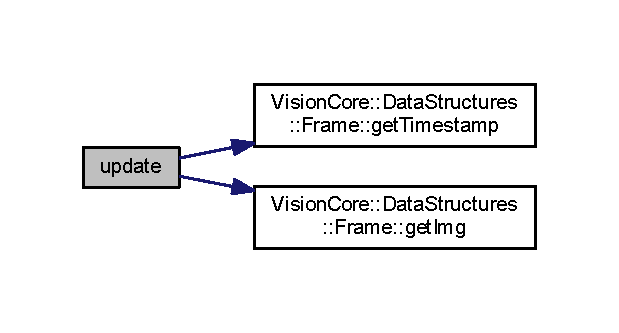
\includegraphics[width=297pt]{class_vision_core_1_1_abstractions_1_1_abstract_auto_tracker_af1a54610c9af7fb54d00e4be2e75609e_cgraph}
\end{center}
\end{figure}




The documentation for this class was generated from the following file\+:\begin{DoxyCompactItemize}
\item 
D\+:/\+F\+U\+R\+G/\+Software/\+Cv\+Works\+Release1/\+Core/\+Vision/Vision\+Abstractions.\+h\end{DoxyCompactItemize}

\hypertarget{class_vision_core_1_1_abstractions_1_1_abstract_particle_filtering_tracker}{}\section{Abstract\+Particle\+Filtering\+Tracker$<$ T\+Img, T\+Obj $>$ Class Template Reference}
\label{class_vision_core_1_1_abstractions_1_1_abstract_particle_filtering_tracker}\index{Abstract\+Particle\+Filtering\+Tracker$<$ T\+Img, T\+Obj $>$@{Abstract\+Particle\+Filtering\+Tracker$<$ T\+Img, T\+Obj $>$}}


Implements a particle filtering algorithm for generic tracking models.  




{\ttfamily \#include $<$Vision\+Abstractions.\+h$>$}



Inheritance diagram for Abstract\+Particle\+Filtering\+Tracker$<$ T\+Img, T\+Obj $>$\+:
\nopagebreak
\begin{figure}[H]
\begin{center}
\leavevmode
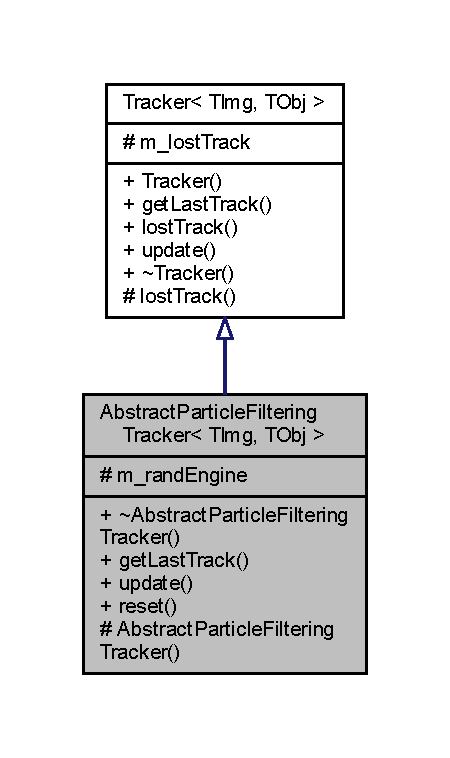
\includegraphics[width=216pt]{class_vision_core_1_1_abstractions_1_1_abstract_particle_filtering_tracker__inherit__graph}
\end{center}
\end{figure}


Collaboration diagram for Abstract\+Particle\+Filtering\+Tracker$<$ T\+Img, T\+Obj $>$\+:
\nopagebreak
\begin{figure}[H]
\begin{center}
\leavevmode
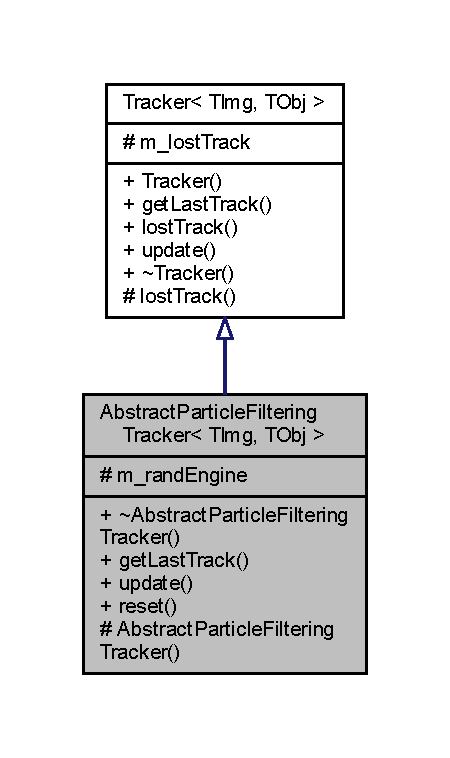
\includegraphics[width=216pt]{class_vision_core_1_1_abstractions_1_1_abstract_particle_filtering_tracker__coll__graph}
\end{center}
\end{figure}
\subsection*{Public Member Functions}
\begin{DoxyCompactItemize}
\item 
\hypertarget{class_vision_core_1_1_abstractions_1_1_abstract_particle_filtering_tracker_ac11a1371779c4e4b8b08c7044a92a3d4}{}virtual \hyperlink{class_vision_core_1_1_abstractions_1_1_abstract_particle_filtering_tracker_ac11a1371779c4e4b8b08c7044a92a3d4}{$\sim$\+Abstract\+Particle\+Filtering\+Tracker} ()\label{class_vision_core_1_1_abstractions_1_1_abstract_particle_filtering_tracker_ac11a1371779c4e4b8b08c7044a92a3d4}

\begin{DoxyCompactList}\small\item\em Destructor method. \end{DoxyCompactList}\item 
virtual const T\+Obj \& \hyperlink{class_vision_core_1_1_abstractions_1_1_abstract_particle_filtering_tracker_a60f002795ee2555f25dc4f7a9a0845ce}{get\+Last\+Track} ()
\begin{DoxyCompactList}\small\item\em Returns a reference to the current estimated object state. \end{DoxyCompactList}\item 
\hypertarget{class_vision_core_1_1_abstractions_1_1_abstract_particle_filtering_tracker_af1a54610c9af7fb54d00e4be2e75609e}{}virtual void \hyperlink{class_vision_core_1_1_abstractions_1_1_abstract_particle_filtering_tracker_af1a54610c9af7fb54d00e4be2e75609e}{update} (const \hyperlink{struct_vision_core_1_1_data_structures_1_1_frame}{Frame}$<$ T\+Img $>$ \&frame)\label{class_vision_core_1_1_abstractions_1_1_abstract_particle_filtering_tracker_af1a54610c9af7fb54d00e4be2e75609e}

\begin{DoxyCompactList}\small\item\em Given an image (i.\+e. video frame), update the tracked objects. \end{DoxyCompactList}\item 
\hypertarget{class_vision_core_1_1_abstractions_1_1_abstract_particle_filtering_tracker_a24876b4e0404782477453810f53fde0b}{}virtual void \hyperlink{class_vision_core_1_1_abstractions_1_1_abstract_particle_filtering_tracker_a24876b4e0404782477453810f53fde0b}{reset} (const T\+Obj \&initial\+Obj)\label{class_vision_core_1_1_abstractions_1_1_abstract_particle_filtering_tracker_a24876b4e0404782477453810f53fde0b}

\begin{DoxyCompactList}\small\item\em Reset the tracked object to a known state. \end{DoxyCompactList}\end{DoxyCompactItemize}
\subsection*{Protected Member Functions}
\begin{DoxyCompactItemize}
\item 
\hypertarget{class_vision_core_1_1_abstractions_1_1_abstract_particle_filtering_tracker_a9ef9b851a62552f9937d57068bb8da8f}{}\hyperlink{class_vision_core_1_1_abstractions_1_1_abstract_particle_filtering_tracker_a9ef9b851a62552f9937d57068bb8da8f}{Abstract\+Particle\+Filtering\+Tracker} (const T\+Obj \&initial\+Obj=T\+Obj(), const unsigned int num\+Particles=100)\label{class_vision_core_1_1_abstractions_1_1_abstract_particle_filtering_tracker_a9ef9b851a62552f9937d57068bb8da8f}

\begin{DoxyCompactList}\small\item\em Constructor method. \end{DoxyCompactList}\end{DoxyCompactItemize}
\subsection*{Protected Attributes}
\begin{DoxyCompactItemize}
\item 
\hypertarget{class_vision_core_1_1_abstractions_1_1_abstract_particle_filtering_tracker_aaeca4119bbd17d828ddc999ffe5d23ea}{}std\+::mt19937 {\bfseries m\+\_\+rand\+Engine}\label{class_vision_core_1_1_abstractions_1_1_abstract_particle_filtering_tracker_aaeca4119bbd17d828ddc999ffe5d23ea}

\end{DoxyCompactItemize}
\subsection*{Additional Inherited Members}


\subsection{Detailed Description}
\subsubsection*{template$<$class T\+Img, class T\+Obj$>$class Vision\+Core\+::\+Abstractions\+::\+Abstract\+Particle\+Filtering\+Tracker$<$ T\+Img, T\+Obj $>$}

Implements a particle filtering algorithm for generic tracking models. 

There are three application specific functions that must be implemented by derived classes\+:
\begin{DoxyItemize}
\item eval\+Obj, which computes the \textquotesingle{}likeliness\textquotesingle{} of a given object be present in the image.
\item sample\+Transition, which generates a new object given a current object.
\item average\+Obj, which performs a weighted combination of several objects.
\end{DoxyItemize}


\begin{DoxyParams}{Parameters}
{\em T\+Img} & The type of input image. \\
\hline
{\em T\+Obj} & The type of object being tracked. \\
\hline
\end{DoxyParams}


Definition at line 847 of file Vision\+Abstractions.\+h.



\subsection{Member Function Documentation}
\hypertarget{class_vision_core_1_1_abstractions_1_1_abstract_particle_filtering_tracker_a60f002795ee2555f25dc4f7a9a0845ce}{}\index{Vision\+Core\+::\+Abstractions\+::\+Abstract\+Particle\+Filtering\+Tracker@{Vision\+Core\+::\+Abstractions\+::\+Abstract\+Particle\+Filtering\+Tracker}!get\+Last\+Track@{get\+Last\+Track}}
\index{get\+Last\+Track@{get\+Last\+Track}!Vision\+Core\+::\+Abstractions\+::\+Abstract\+Particle\+Filtering\+Tracker@{Vision\+Core\+::\+Abstractions\+::\+Abstract\+Particle\+Filtering\+Tracker}}
\subsubsection[{get\+Last\+Track()}]{\setlength{\rightskip}{0pt plus 5cm}const T\+Obj \& get\+Last\+Track (
\begin{DoxyParamCaption}
{}
\end{DoxyParamCaption}
)\hspace{0.3cm}{\ttfamily [virtual]}}\label{class_vision_core_1_1_abstractions_1_1_abstract_particle_filtering_tracker_a60f002795ee2555f25dc4f7a9a0845ce}


Returns a reference to the current estimated object state. 

This function is often call after calling the \hyperlink{class_vision_core_1_1_abstractions_1_1_abstract_particle_filtering_tracker_af1a54610c9af7fb54d00e4be2e75609e}{update()} method. The returned reference is usualy to a class member. 

Implements \hyperlink{class_vision_core_1_1_interfaces_1_1_tracker_a93ee7011307419e8c88db9f22d900657}{Tracker$<$ T\+Img, T\+Obj $>$}.



Definition at line 918 of file Vision\+Abstractions.\+h.



The documentation for this class was generated from the following file\+:\begin{DoxyCompactItemize}
\item 
D\+:/\+F\+U\+R\+G/\+Software/\+Cv\+Works\+Release1/\+Core/\+Vision/Vision\+Abstractions.\+h\end{DoxyCompactItemize}

\hypertarget{class_viscv_1_1_a_r_tag}{}\section{A\+R\+Tag Class Reference}
\label{class_viscv_1_1_a_r_tag}\index{A\+R\+Tag@{A\+R\+Tag}}


Defines a augmented reality tag, which contains a bounding polygon and a tag I\+D.  




{\ttfamily \#include $<$A\+R\+Tag\+Detector\+B\+L\+P.\+h$>$}



Collaboration diagram for A\+R\+Tag\+:
\nopagebreak
\begin{figure}[H]
\begin{center}
\leavevmode
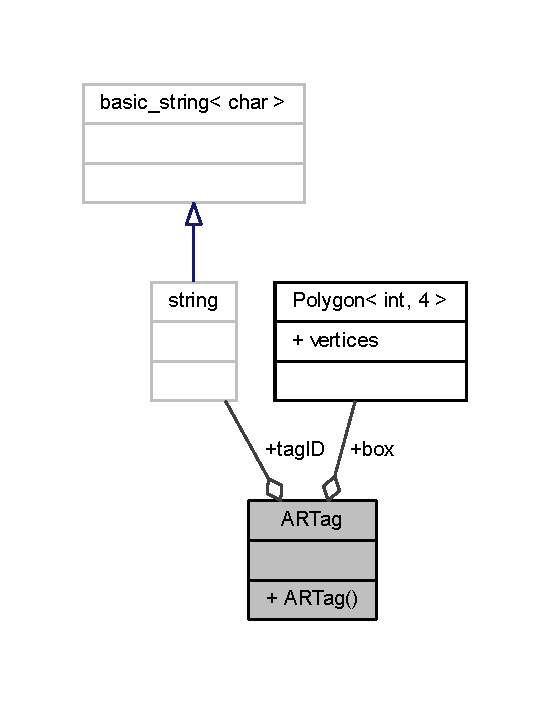
\includegraphics[width=264pt]{class_viscv_1_1_a_r_tag__coll__graph}
\end{center}
\end{figure}
\subsection*{Public Member Functions}
\begin{DoxyCompactItemize}
\item 
\hypertarget{class_viscv_1_1_a_r_tag_a2bcd6453fb99cc398f515a689726a570}{}\hyperlink{class_viscv_1_1_a_r_tag_a2bcd6453fb99cc398f515a689726a570}{A\+R\+Tag} (\hyperlink{class_viscv_1_1_polygon}{Polygon}$<$ int, 4 $>$ box\+\_\+, std\+::string tag\+I\+D\+\_\+)\label{class_viscv_1_1_a_r_tag_a2bcd6453fb99cc398f515a689726a570}

\begin{DoxyCompactList}\small\item\em Construtor. \end{DoxyCompactList}\end{DoxyCompactItemize}
\subsection*{Public Attributes}
\begin{DoxyCompactItemize}
\item 
\hypertarget{class_viscv_1_1_a_r_tag_a26187bbb196ebb1cfc736c275db7a898}{}\hyperlink{class_viscv_1_1_polygon}{Polygon}$<$ int, 4 $>$ \hyperlink{class_viscv_1_1_a_r_tag_a26187bbb196ebb1cfc736c275db7a898}{box}\label{class_viscv_1_1_a_r_tag_a26187bbb196ebb1cfc736c275db7a898}

\begin{DoxyCompactList}\small\item\em \hyperlink{class_viscv_1_1_polygon}{Polygon} that represents the external contour of a tag. \end{DoxyCompactList}\item 
\hypertarget{class_viscv_1_1_a_r_tag_ab8844dfe29ec9d02f624b2459a3c577c}{}std\+::string \hyperlink{class_viscv_1_1_a_r_tag_ab8844dfe29ec9d02f624b2459a3c577c}{tag\+I\+D}\label{class_viscv_1_1_a_r_tag_ab8844dfe29ec9d02f624b2459a3c577c}

\begin{DoxyCompactList}\small\item\em Tag type (I\+D). \end{DoxyCompactList}\end{DoxyCompactItemize}


\subsection{Detailed Description}
Defines a augmented reality tag, which contains a bounding polygon and a tag I\+D. 

Definition at line 44 of file A\+R\+Tag\+Detector\+B\+L\+P.\+h.



The documentation for this class was generated from the following file\+:\begin{DoxyCompactItemize}
\item 
D\+:/\+F\+U\+R\+G/\+Software/\+Cv\+Works\+Release1/\+Components/\+Vision\+Implementation\+Cv/A\+R\+Tag\+Detector\+B\+L\+P.\+h\end{DoxyCompactItemize}

\hypertarget{class_viscv_1_1_a_r_tag_detector_b_l_p}{}\section{A\+R\+Tag\+Detector\+B\+L\+P Class Reference}
\label{class_viscv_1_1_a_r_tag_detector_b_l_p}\index{A\+R\+Tag\+Detector\+B\+L\+P@{A\+R\+Tag\+Detector\+B\+L\+P}}


Implements a augmented reality tag detector.  




{\ttfamily \#include $<$A\+R\+Tag\+Detector\+B\+L\+P.\+h$>$}



Inheritance diagram for A\+R\+Tag\+Detector\+B\+L\+P\+:
\nopagebreak
\begin{figure}[H]
\begin{center}
\leavevmode
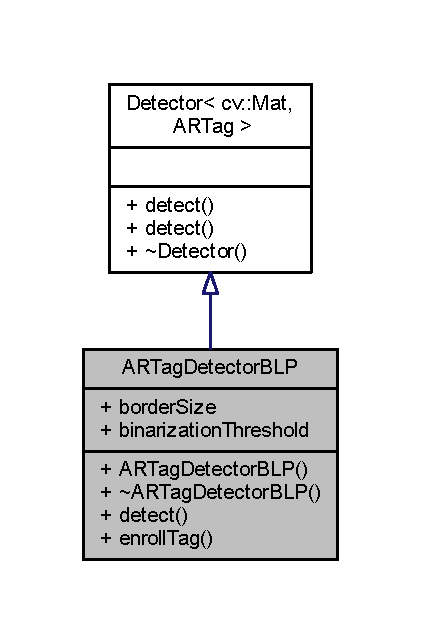
\includegraphics[width=202pt]{class_viscv_1_1_a_r_tag_detector_b_l_p__inherit__graph}
\end{center}
\end{figure}


Collaboration diagram for A\+R\+Tag\+Detector\+B\+L\+P\+:
\nopagebreak
\begin{figure}[H]
\begin{center}
\leavevmode
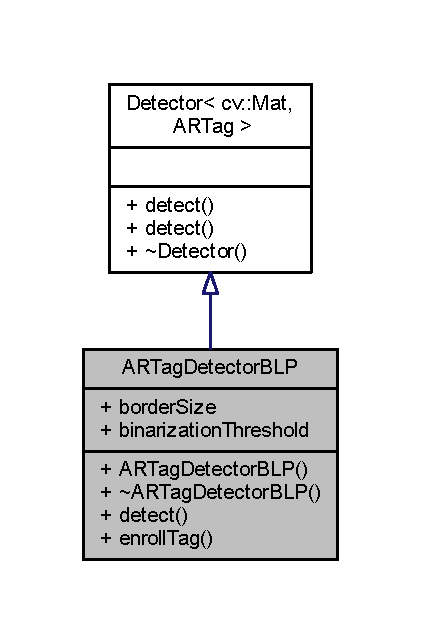
\includegraphics[width=202pt]{class_viscv_1_1_a_r_tag_detector_b_l_p__coll__graph}
\end{center}
\end{figure}
\subsection*{Public Member Functions}
\begin{DoxyCompactItemize}
\item 
\hypertarget{class_viscv_1_1_a_r_tag_detector_b_l_p_a694456c6ce2eaf188d47f4cb61a859b7}{}\hyperlink{class_viscv_1_1_a_r_tag_detector_b_l_p_a694456c6ce2eaf188d47f4cb61a859b7}{A\+R\+Tag\+Detector\+B\+L\+P} ()\label{class_viscv_1_1_a_r_tag_detector_b_l_p_a694456c6ce2eaf188d47f4cb61a859b7}

\begin{DoxyCompactList}\small\item\em Defult constructor. \end{DoxyCompactList}\item 
\hypertarget{class_viscv_1_1_a_r_tag_detector_b_l_p_aac8748a45253d9b678b66b5ce8ac0edd}{}\hyperlink{class_viscv_1_1_a_r_tag_detector_b_l_p_aac8748a45253d9b678b66b5ce8ac0edd}{$\sim$\+A\+R\+Tag\+Detector\+B\+L\+P} ()\label{class_viscv_1_1_a_r_tag_detector_b_l_p_aac8748a45253d9b678b66b5ce8ac0edd}

\begin{DoxyCompactList}\small\item\em Destructor. \end{DoxyCompactList}\item 
std\+::vector$<$ \hyperlink{class_viscv_1_1_a_r_tag}{A\+R\+Tag} $>$ \hyperlink{class_viscv_1_1_a_r_tag_detector_b_l_p_a0065a0a0e3dbed236849bf406e6cde66}{detect} (const cv\+::\+Mat \&img) const 
\begin{DoxyCompactList}\small\item\em Detects objects in the image and returns a vector with the detected objects. \end{DoxyCompactList}\item 
\hypertarget{class_viscv_1_1_a_r_tag_detector_b_l_p_a71fdd952985e3be53e73443a02b07cfe}{}void \hyperlink{class_viscv_1_1_a_r_tag_detector_b_l_p_a71fdd952985e3be53e73443a02b07cfe}{enroll\+Tag} (const cv\+::\+Mat \&tag\+Img, const std\+::string \&tag\+Name)\label{class_viscv_1_1_a_r_tag_detector_b_l_p_a71fdd952985e3be53e73443a02b07cfe}

\begin{DoxyCompactList}\small\item\em Enrolls new tags. \end{DoxyCompactList}\end{DoxyCompactItemize}
\subsection*{Public Attributes}
\begin{DoxyCompactItemize}
\item 
\hypertarget{class_viscv_1_1_a_r_tag_detector_b_l_p_acc427385dd28416f812523874f4d6502}{}int \hyperlink{class_viscv_1_1_a_r_tag_detector_b_l_p_acc427385dd28416f812523874f4d6502}{border\+Size}\label{class_viscv_1_1_a_r_tag_detector_b_l_p_acc427385dd28416f812523874f4d6502}

\begin{DoxyCompactList}\small\item\em Tag border size. \end{DoxyCompactList}\item 
\hypertarget{class_viscv_1_1_a_r_tag_detector_b_l_p_a0ebf501c4c0e6e53d9695a43466ea184}{}int \hyperlink{class_viscv_1_1_a_r_tag_detector_b_l_p_a0ebf501c4c0e6e53d9695a43466ea184}{binarization\+Threshold}\label{class_viscv_1_1_a_r_tag_detector_b_l_p_a0ebf501c4c0e6e53d9695a43466ea184}

\begin{DoxyCompactList}\small\item\em Threshold used in image binarization. \end{DoxyCompactList}\end{DoxyCompactItemize}
\subsection*{Additional Inherited Members}


\subsection{Detailed Description}
Implements a augmented reality tag detector. 

This algorith is similar to the one implemented in A\+R\+Toolkit. It first detects a bounding polygon around a tag. Then it extract the image inside the tag and match it agains a set of enrolled tags (see enroll\+Tag method), assigning the tag with higher similarity. \begin{Desc}
\item[Examples\+: ]\par
\hyperlink{_vision_tests_2main_8cpp-example}{Vision\+Tests/main.\+cpp}.\end{Desc}


Definition at line 70 of file A\+R\+Tag\+Detector\+B\+L\+P.\+h.



\subsection{Member Function Documentation}
\hypertarget{class_viscv_1_1_a_r_tag_detector_b_l_p_a0065a0a0e3dbed236849bf406e6cde66}{}\index{Viscv\+::\+A\+R\+Tag\+Detector\+B\+L\+P@{Viscv\+::\+A\+R\+Tag\+Detector\+B\+L\+P}!detect@{detect}}
\index{detect@{detect}!Viscv\+::\+A\+R\+Tag\+Detector\+B\+L\+P@{Viscv\+::\+A\+R\+Tag\+Detector\+B\+L\+P}}
\subsubsection[{detect(const cv\+::\+Mat \&img) const }]{\setlength{\rightskip}{0pt plus 5cm}std\+::vector$<$ {\bf A\+R\+Tag} $>$ detect (
\begin{DoxyParamCaption}
\item[{const cv\+::\+Mat \&}]{img}
\end{DoxyParamCaption}
) const\hspace{0.3cm}{\ttfamily [virtual]}}\label{class_viscv_1_1_a_r_tag_detector_b_l_p_a0065a0a0e3dbed236849bf406e6cde66}


Detects objects in the image and returns a vector with the detected objects. 

The vector should be empty if no object is detected. 

Implements \hyperlink{class_vision_core_1_1_interfaces_1_1_detector_a0977745b253f810bb2ec009844618305}{Detector$<$ cv\+::\+Mat, A\+R\+Tag $>$}.

\begin{Desc}
\item[Examples\+: ]\par
\hyperlink{_vision_tests_2main_8cpp-example}{Vision\+Tests/main.\+cpp}.\end{Desc}


Definition at line 54 of file A\+R\+Tag\+Detector\+B\+L\+P.\+cpp.



The documentation for this class was generated from the following files\+:\begin{DoxyCompactItemize}
\item 
D\+:/\+F\+U\+R\+G/\+Software/\+Cv\+Works\+Release1/\+Components/\+Vision\+Implementation\+Cv/A\+R\+Tag\+Detector\+B\+L\+P.\+h\item 
D\+:/\+F\+U\+R\+G/\+Software/\+Cv\+Works\+Release1/\+Components/\+Vision\+Implementation\+Cv/A\+R\+Tag\+Detector\+B\+L\+P.\+cpp\end{DoxyCompactItemize}

\hypertarget{class_vision_core_1_1_async_1_1_async_detector_wrap}{}\section{Async\+Detector\+Wrap$<$ T\+Img, T\+Obj $>$ Class Template Reference}
\label{class_vision_core_1_1_async_1_1_async_detector_wrap}\index{Async\+Detector\+Wrap$<$ T\+Img, T\+Obj $>$@{Async\+Detector\+Wrap$<$ T\+Img, T\+Obj $>$}}


Allows the execution of a detector asynchronously in an individual thread.  




{\ttfamily \#include $<$Vision\+Async.\+h$>$}



Inheritance diagram for Async\+Detector\+Wrap$<$ T\+Img, T\+Obj $>$\+:
\nopagebreak
\begin{figure}[H]
\begin{center}
\leavevmode
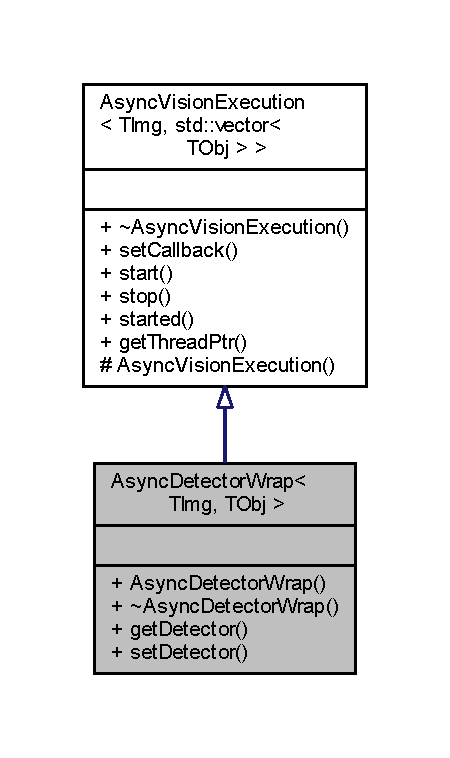
\includegraphics[width=216pt]{class_vision_core_1_1_async_1_1_async_detector_wrap__inherit__graph}
\end{center}
\end{figure}


Collaboration diagram for Async\+Detector\+Wrap$<$ T\+Img, T\+Obj $>$\+:
\nopagebreak
\begin{figure}[H]
\begin{center}
\leavevmode
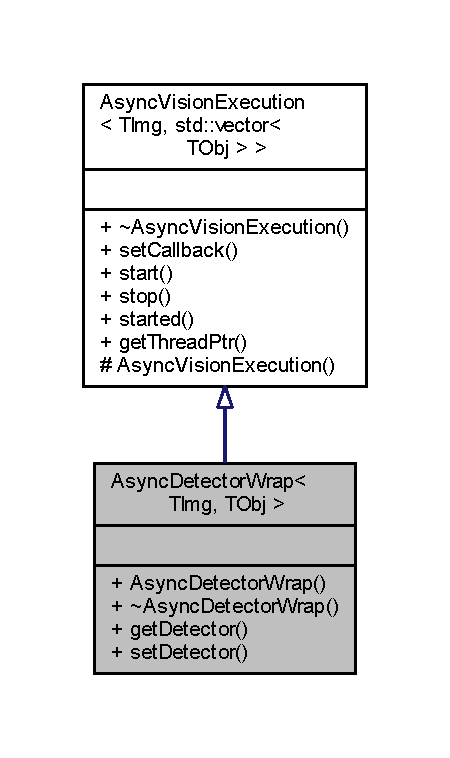
\includegraphics[width=216pt]{class_vision_core_1_1_async_1_1_async_detector_wrap__coll__graph}
\end{center}
\end{figure}
\subsection*{Public Member Functions}
\begin{DoxyCompactItemize}
\item 
\hyperlink{class_vision_core_1_1_async_1_1_async_detector_wrap_a2b7d5e050fbeba8a1fbbda53258c041e}{Async\+Detector\+Wrap} (\hyperlink{class_vision_core_1_1_async_1_1_async_frame_server_wrap}{Async\+Frame\+Server\+Wrap}$<$ T\+Img $>$ $\ast$afs\+Ptr, const \hyperlink{class_vision_core_1_1_interfaces_1_1_detector}{Detector}$<$ T\+Img, T\+Obj $>$ $\ast$detector)
\begin{DoxyCompactList}\small\item\em Constructor method. \end{DoxyCompactList}\item 
\hypertarget{class_vision_core_1_1_async_1_1_async_detector_wrap_a6c965557375c470298058247830c1633}{}const \hyperlink{class_vision_core_1_1_interfaces_1_1_detector}{Detector}$<$ T\+Img, T\+Obj $>$ $\ast$ {\bfseries get\+Detector} () const \label{class_vision_core_1_1_async_1_1_async_detector_wrap_a6c965557375c470298058247830c1633}

\item 
\hypertarget{class_vision_core_1_1_async_1_1_async_detector_wrap_a2d06cfb8e49df174b8315898a0e4e3c7}{}void {\bfseries set\+Detector} (const \hyperlink{class_vision_core_1_1_interfaces_1_1_detector}{Detector}$<$ T\+Img, T\+Obj $>$ $\ast$Sdetector)\label{class_vision_core_1_1_async_1_1_async_detector_wrap_a2d06cfb8e49df174b8315898a0e4e3c7}

\end{DoxyCompactItemize}
\subsection*{Additional Inherited Members}


\subsection{Detailed Description}
\subsubsection*{template$<$class T\+Img, class T\+Obj$>$class Vision\+Core\+::\+Async\+::\+Async\+Detector\+Wrap$<$ T\+Img, T\+Obj $>$}

Allows the execution of a detector asynchronously in an individual thread. 

This class is a wrap for a Detector object. It listens an \hyperlink{class_vision_core_1_1_async_1_1_async_frame_server_wrap}{Async\+Frame\+Server\+Wrap} object (given in the constructor) and, when a new frame becomes available, it executes the object detection.

After every detection, the results are passed to a user provided callback function (see set\+Calback).

The detector runs in a exclusive internal thread.


\begin{DoxyParams}{Parameters}
{\em T\+Img} & Image type. \\
\hline
{\em T\+Obj} & Object type. \\
\hline
\end{DoxyParams}


Definition at line 437 of file Vision\+Async.\+h.



\subsection{Constructor \& Destructor Documentation}
\hypertarget{class_vision_core_1_1_async_1_1_async_detector_wrap_a2b7d5e050fbeba8a1fbbda53258c041e}{}\index{Vision\+Core\+::\+Async\+::\+Async\+Detector\+Wrap@{Vision\+Core\+::\+Async\+::\+Async\+Detector\+Wrap}!Async\+Detector\+Wrap@{Async\+Detector\+Wrap}}
\index{Async\+Detector\+Wrap@{Async\+Detector\+Wrap}!Vision\+Core\+::\+Async\+::\+Async\+Detector\+Wrap@{Vision\+Core\+::\+Async\+::\+Async\+Detector\+Wrap}}
\subsubsection[{Async\+Detector\+Wrap(\+Async\+Frame\+Server\+Wrap$<$ T\+Img $>$ $\ast$afs\+Ptr, const Detector$<$ T\+Img, T\+Obj $>$ $\ast$detector)}]{\setlength{\rightskip}{0pt plus 5cm}{\bf Async\+Detector\+Wrap} (
\begin{DoxyParamCaption}
\item[{{\bf Async\+Frame\+Server\+Wrap}$<$ T\+Img $>$ $\ast$}]{afs\+Ptr, }
\item[{const {\bf Detector}$<$ T\+Img, T\+Obj $>$ $\ast$}]{detector}
\end{DoxyParamCaption}
)}\label{class_vision_core_1_1_async_1_1_async_detector_wrap_a2b7d5e050fbeba8a1fbbda53258c041e}


Constructor method. 

The user should provide a pointer to a async frame server, that will be listened for new frames, and a detector, that will be executed on every captured frame. 

Definition at line 461 of file Vision\+Async.\+h.



The documentation for this class was generated from the following file\+:\begin{DoxyCompactItemize}
\item 
D\+:/\+F\+U\+R\+G/\+Software/\+Cv\+Works\+Release1/\+Core/\+Vision/Vision\+Async.\+h\end{DoxyCompactItemize}

\hypertarget{class_vision_core_1_1_async_1_1_async_frame_server_wrap}{}\section{Async\+Frame\+Server\+Wrap$<$ T\+Img $>$ Class Template Reference}
\label{class_vision_core_1_1_async_1_1_async_frame_server_wrap}\index{Async\+Frame\+Server\+Wrap$<$ T\+Img $>$@{Async\+Frame\+Server\+Wrap$<$ T\+Img $>$}}


Allows the execution of a frame server asynchronously in an individual thread.  




{\ttfamily \#include $<$Vision\+Async.\+h$>$}



Collaboration diagram for Async\+Frame\+Server\+Wrap$<$ T\+Img $>$\+:
\nopagebreak
\begin{figure}[H]
\begin{center}
\leavevmode
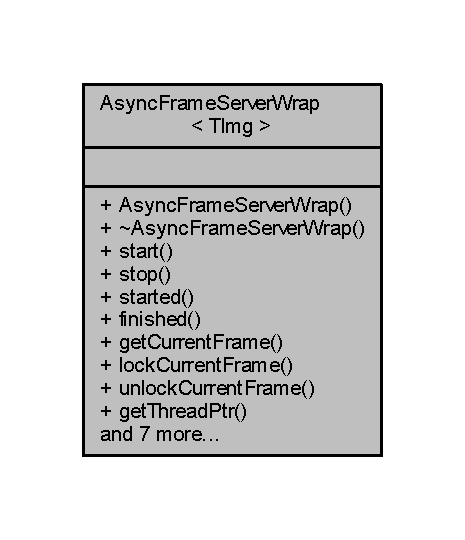
\includegraphics[width=223pt]{class_vision_core_1_1_async_1_1_async_frame_server_wrap__coll__graph}
\end{center}
\end{figure}
\subsection*{Public Member Functions}
\begin{DoxyCompactItemize}
\item 
\hypertarget{class_vision_core_1_1_async_1_1_async_frame_server_wrap_ae8ba94875d13625942e6e478b28fc19b}{}\hyperlink{class_vision_core_1_1_async_1_1_async_frame_server_wrap_ae8ba94875d13625942e6e478b28fc19b}{Async\+Frame\+Server\+Wrap} (\hyperlink{class_vision_core_1_1_interfaces_1_1_frame_server}{Frame\+Server}$<$ T\+Img $>$ $\ast$frame\+Server, int frames\+Per\+Second=-\/1)\label{class_vision_core_1_1_async_1_1_async_frame_server_wrap_ae8ba94875d13625942e6e478b28fc19b}

\begin{DoxyCompactList}\small\item\em Constructor. \end{DoxyCompactList}\item 
\hypertarget{class_vision_core_1_1_async_1_1_async_frame_server_wrap_a04c264bb27b2ac35a81be42f772e0b52}{}virtual \hyperlink{class_vision_core_1_1_async_1_1_async_frame_server_wrap_a04c264bb27b2ac35a81be42f772e0b52}{$\sim$\+Async\+Frame\+Server\+Wrap} ()\label{class_vision_core_1_1_async_1_1_async_frame_server_wrap_a04c264bb27b2ac35a81be42f772e0b52}

\begin{DoxyCompactList}\small\item\em Destructor method. \end{DoxyCompactList}\item 
void \hyperlink{class_vision_core_1_1_async_1_1_async_frame_server_wrap_a60de64d75454385b23995437f1d72669}{start} ()
\begin{DoxyCompactList}\small\item\em Start frame capturing in a individual thread. \end{DoxyCompactList}\item 
\hypertarget{class_vision_core_1_1_async_1_1_async_frame_server_wrap_a8c528baf37154d347366083f0f816846}{}void \hyperlink{class_vision_core_1_1_async_1_1_async_frame_server_wrap_a8c528baf37154d347366083f0f816846}{stop} ()\label{class_vision_core_1_1_async_1_1_async_frame_server_wrap_a8c528baf37154d347366083f0f816846}

\begin{DoxyCompactList}\small\item\em Stops the capture of new frames (works as a pause). \end{DoxyCompactList}\item 
\hypertarget{class_vision_core_1_1_async_1_1_async_frame_server_wrap_ade061155643ea9800e0d385caa9ddc5a}{}bool \hyperlink{class_vision_core_1_1_async_1_1_async_frame_server_wrap_ade061155643ea9800e0d385caa9ddc5a}{started} () const \label{class_vision_core_1_1_async_1_1_async_frame_server_wrap_ade061155643ea9800e0d385caa9ddc5a}

\begin{DoxyCompactList}\small\item\em Indicates if the frames are being captured. \end{DoxyCompactList}\item 
\hypertarget{class_vision_core_1_1_async_1_1_async_frame_server_wrap_a8222e52df762c74ec229eba833a6d310}{}bool \hyperlink{class_vision_core_1_1_async_1_1_async_frame_server_wrap_a8222e52df762c74ec229eba833a6d310}{finished} () const \label{class_vision_core_1_1_async_1_1_async_frame_server_wrap_a8222e52df762c74ec229eba833a6d310}

\begin{DoxyCompactList}\small\item\em Indicates if the video reached the end. \end{DoxyCompactList}\item 
\hypertarget{class_vision_core_1_1_async_1_1_async_frame_server_wrap_a954ec16b07c6dffd3e6fa1c19adde9a7}{}std\+::shared\+\_\+ptr$<$ \hyperlink{struct_vision_core_1_1_data_structures_1_1_frame}{Frame}$<$ T\+Img $>$ $>$ \hyperlink{class_vision_core_1_1_async_1_1_async_frame_server_wrap_a954ec16b07c6dffd3e6fa1c19adde9a7}{get\+Current\+Frame} ()\label{class_vision_core_1_1_async_1_1_async_frame_server_wrap_a954ec16b07c6dffd3e6fa1c19adde9a7}

\begin{DoxyCompactList}\small\item\em Returns the most recent captured frame. \end{DoxyCompactList}\item 
\hypertarget{class_vision_core_1_1_async_1_1_async_frame_server_wrap_a142af7cc4e4839ba5f6db05cc3f5d783}{}void \hyperlink{class_vision_core_1_1_async_1_1_async_frame_server_wrap_a142af7cc4e4839ba5f6db05cc3f5d783}{lock\+Current\+Frame} ()\label{class_vision_core_1_1_async_1_1_async_frame_server_wrap_a142af7cc4e4839ba5f6db05cc3f5d783}

\begin{DoxyCompactList}\small\item\em Blocks the access to last captured frame to the trhead that called this function. \end{DoxyCompactList}\item 
\hypertarget{class_vision_core_1_1_async_1_1_async_frame_server_wrap_a246fb6f2273f5066fab7e6cfcb01f322}{}void \hyperlink{class_vision_core_1_1_async_1_1_async_frame_server_wrap_a246fb6f2273f5066fab7e6cfcb01f322}{unlock\+Current\+Frame} ()\label{class_vision_core_1_1_async_1_1_async_frame_server_wrap_a246fb6f2273f5066fab7e6cfcb01f322}

\begin{DoxyCompactList}\small\item\em Releases the captured frames to other threads. \end{DoxyCompactList}\item 
\hypertarget{class_vision_core_1_1_async_1_1_async_frame_server_wrap_abd8ac6727051c47ac2b8d695efc63603}{}std\+::thread $\ast$ \hyperlink{class_vision_core_1_1_async_1_1_async_frame_server_wrap_abd8ac6727051c47ac2b8d695efc63603}{get\+Thread\+Ptr} ()\label{class_vision_core_1_1_async_1_1_async_frame_server_wrap_abd8ac6727051c47ac2b8d695efc63603}

\begin{DoxyCompactList}\small\item\em Returns a pointer to the internal thread exececuting frame capture. \end{DoxyCompactList}\item 
\hypertarget{class_vision_core_1_1_async_1_1_async_frame_server_wrap_a2f76fa0062ff4d405b8296b356ec6833}{}std\+::condition\+\_\+variable \& \hyperlink{class_vision_core_1_1_async_1_1_async_frame_server_wrap_a2f76fa0062ff4d405b8296b356ec6833}{get\+New\+Frame\+Cond\+Var} ()\label{class_vision_core_1_1_async_1_1_async_frame_server_wrap_a2f76fa0062ff4d405b8296b356ec6833}

\begin{DoxyCompactList}\small\item\em Returns the conditional variable used to notify other threads that a new frame was captured. \end{DoxyCompactList}\item 
\hypertarget{class_vision_core_1_1_async_1_1_async_frame_server_wrap_a6c5641dc8b269eee5a0bf7d2e47ed9ed}{}void \hyperlink{class_vision_core_1_1_async_1_1_async_frame_server_wrap_a6c5641dc8b269eee5a0bf7d2e47ed9ed}{set\+Callback} (const std\+::function$<$ void(std\+::shared\+\_\+ptr$<$ \hyperlink{struct_vision_core_1_1_data_structures_1_1_frame}{Frame}$<$ T\+Img $>$$>$)$>$ \&callback)\label{class_vision_core_1_1_async_1_1_async_frame_server_wrap_a6c5641dc8b269eee5a0bf7d2e47ed9ed}

\begin{DoxyCompactList}\small\item\em Sets a callback function that is executed after every frame capture. \end{DoxyCompactList}\item 
\hypertarget{class_vision_core_1_1_async_1_1_async_frame_server_wrap_ae765905307a24758f1ed460be1fd80b2}{}void \hyperlink{class_vision_core_1_1_async_1_1_async_frame_server_wrap_ae765905307a24758f1ed460be1fd80b2}{add\+Callback} (const std\+::function$<$ void(std\+::shared\+\_\+ptr$<$ \hyperlink{struct_vision_core_1_1_data_structures_1_1_frame}{Frame}$<$ T\+Img $>$$>$)$>$ \&callback)\label{class_vision_core_1_1_async_1_1_async_frame_server_wrap_ae765905307a24758f1ed460be1fd80b2}

\begin{DoxyCompactList}\small\item\em Add a callback function that is executed after each capture. \end{DoxyCompactList}\item 
\hypertarget{class_vision_core_1_1_async_1_1_async_frame_server_wrap_ab212e28ba94abfba3af5cea45609a502}{}void \hyperlink{class_vision_core_1_1_async_1_1_async_frame_server_wrap_ab212e28ba94abfba3af5cea45609a502}{set\+Frames\+To\+Capture} (const int quantity)\label{class_vision_core_1_1_async_1_1_async_frame_server_wrap_ab212e28ba94abfba3af5cea45609a502}

\begin{DoxyCompactList}\small\item\em Sets how many frames will be captured. The frame server will pause(stop) after capturing these frames. Negative values means no restriction. \end{DoxyCompactList}\item 
\hypertarget{class_vision_core_1_1_async_1_1_async_frame_server_wrap_a064142ef99cfb7aaad5ba4eb51056ab7}{}void \hyperlink{class_vision_core_1_1_async_1_1_async_frame_server_wrap_a064142ef99cfb7aaad5ba4eb51056ab7}{set\+Frame\+Server} (\hyperlink{class_vision_core_1_1_interfaces_1_1_frame_server}{Frame\+Server}$<$ T\+Img $>$ $\ast$fs)\label{class_vision_core_1_1_async_1_1_async_frame_server_wrap_a064142ef99cfb7aaad5ba4eb51056ab7}

\begin{DoxyCompactList}\small\item\em Sets a new frame server. The old is not deleted. \end{DoxyCompactList}\item 
\hypertarget{class_vision_core_1_1_async_1_1_async_frame_server_wrap_aa4d334f33f49c61c9b3e306b60f4cc74}{}double \hyperlink{class_vision_core_1_1_async_1_1_async_frame_server_wrap_aa4d334f33f49c61c9b3e306b60f4cc74}{get\+Frames\+Per\+Second} () const \label{class_vision_core_1_1_async_1_1_async_frame_server_wrap_aa4d334f33f49c61c9b3e306b60f4cc74}

\begin{DoxyCompactList}\small\item\em Get the frames captured per second. \end{DoxyCompactList}\item 
\hypertarget{class_vision_core_1_1_async_1_1_async_frame_server_wrap_a0d21ea1dd98cb2913cef820c71ab1e54}{}void \hyperlink{class_vision_core_1_1_async_1_1_async_frame_server_wrap_a0d21ea1dd98cb2913cef820c71ab1e54}{set\+Frames\+Per\+Second} (double frames\+Per\+Second)\label{class_vision_core_1_1_async_1_1_async_frame_server_wrap_a0d21ea1dd98cb2913cef820c71ab1e54}

\begin{DoxyCompactList}\small\item\em Sets the frames captured per second. If it is less or equal to 0 the capture will be as fast as possible (may be problematic for other threads processing the frames). \end{DoxyCompactList}\end{DoxyCompactItemize}


\subsection{Detailed Description}
\subsubsection*{template$<$class T\+Img$>$class Vision\+Core\+::\+Async\+::\+Async\+Frame\+Server\+Wrap$<$ T\+Img $>$}

Allows the execution of a frame server asynchronously in an individual thread. 

This class is a wrap for a Frame\+Server object that captures frames in a individual thread and notifies other trheads the frame capture (using std conditional variables). This way, other threads can access the captured frames by calling the \hyperlink{class_vision_core_1_1_async_1_1_async_frame_server_wrap_a954ec16b07c6dffd3e6fa1c19adde9a7}{get\+Current\+Frame()} method.

It is also possible to set a callback function (\hyperlink{class_vision_core_1_1_async_1_1_async_frame_server_wrap_a6c5641dc8b269eee5a0bf7d2e47ed9ed}{set\+Callback()} method) that is executed after every frame capture.\+s.


\begin{DoxyParams}{Parameters}
{\em T\+Img} & Image type. \\
\hline
\end{DoxyParams}


Definition at line 64 of file Vision\+Async.\+h.



\subsection{Member Function Documentation}
\hypertarget{class_vision_core_1_1_async_1_1_async_frame_server_wrap_a60de64d75454385b23995437f1d72669}{}\index{Vision\+Core\+::\+Async\+::\+Async\+Frame\+Server\+Wrap@{Vision\+Core\+::\+Async\+::\+Async\+Frame\+Server\+Wrap}!start@{start}}
\index{start@{start}!Vision\+Core\+::\+Async\+::\+Async\+Frame\+Server\+Wrap@{Vision\+Core\+::\+Async\+::\+Async\+Frame\+Server\+Wrap}}
\subsubsection[{start()}]{\setlength{\rightskip}{0pt plus 5cm}void start (
\begin{DoxyParamCaption}
{}
\end{DoxyParamCaption}
)\hspace{0.3cm}{\ttfamily [inline]}}\label{class_vision_core_1_1_async_1_1_async_frame_server_wrap_a60de64d75454385b23995437f1d72669}


Start frame capturing in a individual thread. 

The frames are captured from the internal Frame\+Server object continuously. While capturing is active, other threads are notified of a capture using the conditional variable. 

Definition at line 77 of file Vision\+Async.\+h.



The documentation for this class was generated from the following file\+:\begin{DoxyCompactItemize}
\item 
D\+:/\+F\+U\+R\+G/\+Software/\+Cv\+Works\+Release1/\+Core/\+Vision/Vision\+Async.\+h\end{DoxyCompactItemize}

\hypertarget{class_vision_core_1_1_async_1_1_async_tracker_wrap}{}\section{Async\+Tracker\+Wrap$<$ T\+Img, T\+Obj $>$ Class Template Reference}
\label{class_vision_core_1_1_async_1_1_async_tracker_wrap}\index{Async\+Tracker\+Wrap$<$ T\+Img, T\+Obj $>$@{Async\+Tracker\+Wrap$<$ T\+Img, T\+Obj $>$}}


Allows the execution of a tracker asynchronously in an individual thread.  




{\ttfamily \#include $<$Vision\+Async.\+h$>$}



Inheritance diagram for Async\+Tracker\+Wrap$<$ T\+Img, T\+Obj $>$\+:
\nopagebreak
\begin{figure}[H]
\begin{center}
\leavevmode
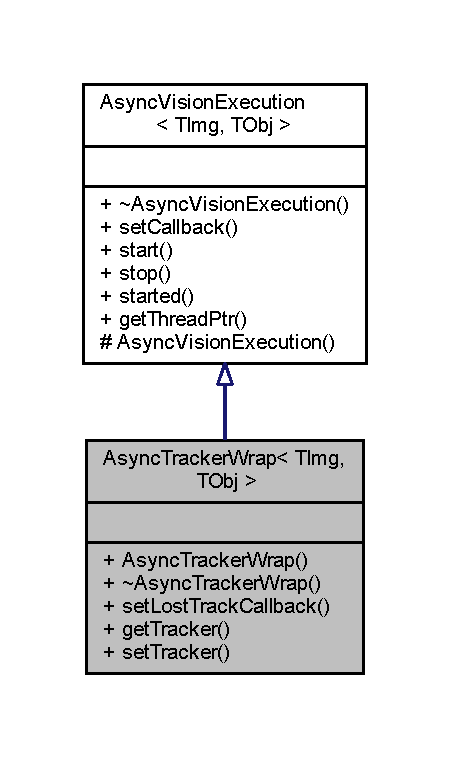
\includegraphics[width=216pt]{class_vision_core_1_1_async_1_1_async_tracker_wrap__inherit__graph}
\end{center}
\end{figure}


Collaboration diagram for Async\+Tracker\+Wrap$<$ T\+Img, T\+Obj $>$\+:
\nopagebreak
\begin{figure}[H]
\begin{center}
\leavevmode
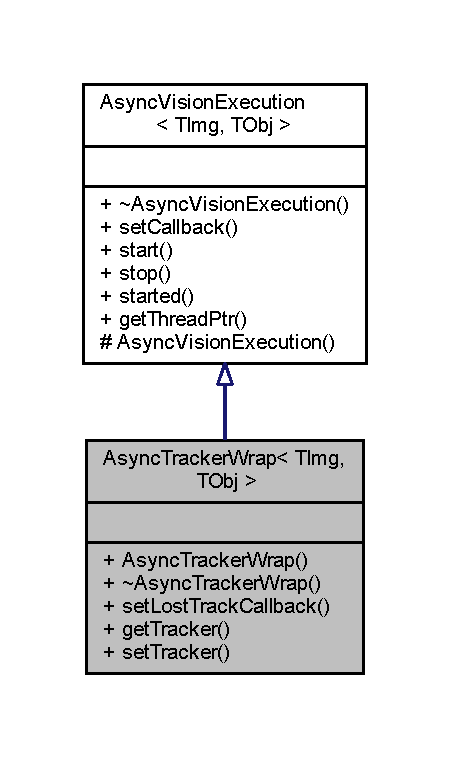
\includegraphics[width=216pt]{class_vision_core_1_1_async_1_1_async_tracker_wrap__coll__graph}
\end{center}
\end{figure}
\subsection*{Public Member Functions}
\begin{DoxyCompactItemize}
\item 
\hypertarget{class_vision_core_1_1_async_1_1_async_tracker_wrap_a1a4463f9a48cbd9bd54494d430d9f656}{}\hyperlink{class_vision_core_1_1_async_1_1_async_tracker_wrap_a1a4463f9a48cbd9bd54494d430d9f656}{Async\+Tracker\+Wrap} (\hyperlink{class_vision_core_1_1_async_1_1_async_frame_server_wrap}{Async\+Frame\+Server\+Wrap}$<$ T\+Img $>$ $\ast$afs\+Ptr, \hyperlink{class_vision_core_1_1_interfaces_1_1_tracker}{Tracker}$<$ T\+Img, T\+Obj $>$ $\ast$tracker)\label{class_vision_core_1_1_async_1_1_async_tracker_wrap_a1a4463f9a48cbd9bd54494d430d9f656}

\begin{DoxyCompactList}\small\item\em Constructor method. \end{DoxyCompactList}\item 
\hypertarget{class_vision_core_1_1_async_1_1_async_tracker_wrap_a39c25715a3846239ec1380955fb49e19}{}void \hyperlink{class_vision_core_1_1_async_1_1_async_tracker_wrap_a39c25715a3846239ec1380955fb49e19}{set\+Lost\+Track\+Callback} (const std\+::function$<$ void()$>$ \&r\+Callback)\label{class_vision_core_1_1_async_1_1_async_tracker_wrap_a39c25715a3846239ec1380955fb49e19}

\begin{DoxyCompactList}\small\item\em Set the lost track callback. \end{DoxyCompactList}\item 
\hypertarget{class_vision_core_1_1_async_1_1_async_tracker_wrap_a67d8937141cc8d2766bc0119a4eabe21}{}\hyperlink{class_vision_core_1_1_interfaces_1_1_tracker}{Tracker}$<$ T\+Img, T\+Obj $>$ $\ast$ {\bfseries get\+Tracker} () const \label{class_vision_core_1_1_async_1_1_async_tracker_wrap_a67d8937141cc8d2766bc0119a4eabe21}

\item 
\hypertarget{class_vision_core_1_1_async_1_1_async_tracker_wrap_a9556d32505a461b5af0782dfe13e2bce}{}void {\bfseries set\+Tracker} (\hyperlink{class_vision_core_1_1_interfaces_1_1_tracker}{Tracker}$<$ T\+Img, T\+Obj $>$ $\ast$tracker)\label{class_vision_core_1_1_async_1_1_async_tracker_wrap_a9556d32505a461b5af0782dfe13e2bce}

\end{DoxyCompactItemize}
\subsection*{Additional Inherited Members}


\subsection{Detailed Description}
\subsubsection*{template$<$class T\+Img, class T\+Obj$>$class Vision\+Core\+::\+Async\+::\+Async\+Tracker\+Wrap$<$ T\+Img, T\+Obj $>$}

Allows the execution of a tracker asynchronously in an individual thread. 

This class is a wrap for a Tracker object. It listens an \hyperlink{class_vision_core_1_1_async_1_1_async_frame_server_wrap}{Async\+Frame\+Server\+Wrap} object (given in the constructor) and, when a new frame becomes available, it updates the tracker.

After every tracker update, the result (i.\+e. current tracked object position) is passed to a user provided callback function (see set\+Calback).

The tracker runs in a exclusive internal thread.


\begin{DoxyParams}{Parameters}
{\em T\+Img} & Image type. \\
\hline
{\em T\+Obj} & Object type. \\
\hline
\end{DoxyParams}


Definition at line 506 of file Vision\+Async.\+h.



The documentation for this class was generated from the following file\+:\begin{DoxyCompactItemize}
\item 
D\+:/\+F\+U\+R\+G/\+Software/\+Cv\+Works\+Release1/\+Core/\+Vision/Vision\+Async.\+h\end{DoxyCompactItemize}

\hypertarget{class_vision_core_1_1_async_1_1_async_vision_execution}{}\section{Async\+Vision\+Execution$<$ T\+Img, T\+Out $>$ Class Template Reference}
\label{class_vision_core_1_1_async_1_1_async_vision_execution}\index{Async\+Vision\+Execution$<$ T\+Img, T\+Out $>$@{Async\+Vision\+Execution$<$ T\+Img, T\+Out $>$}}


Allows the execution of a vision method asynchronously in an individual thread.  




{\ttfamily \#include $<$Vision\+Async.\+h$>$}



Collaboration diagram for Async\+Vision\+Execution$<$ T\+Img, T\+Out $>$\+:
\nopagebreak
\begin{figure}[H]
\begin{center}
\leavevmode
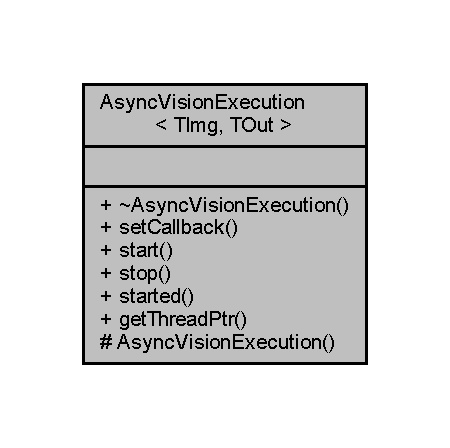
\includegraphics[width=216pt]{class_vision_core_1_1_async_1_1_async_vision_execution__coll__graph}
\end{center}
\end{figure}
\subsection*{Public Member Functions}
\begin{DoxyCompactItemize}
\item 
\hypertarget{class_vision_core_1_1_async_1_1_async_vision_execution_a7c6b158b64e320c959e8bf6c5aeae822}{}virtual \hyperlink{class_vision_core_1_1_async_1_1_async_vision_execution_a7c6b158b64e320c959e8bf6c5aeae822}{$\sim$\+Async\+Vision\+Execution} ()\label{class_vision_core_1_1_async_1_1_async_vision_execution_a7c6b158b64e320c959e8bf6c5aeae822}

\begin{DoxyCompactList}\small\item\em Destructor method. \end{DoxyCompactList}\item 
\hypertarget{class_vision_core_1_1_async_1_1_async_vision_execution_aa6308ff596cc79d9feae867931dc5df2}{}void \hyperlink{class_vision_core_1_1_async_1_1_async_vision_execution_aa6308ff596cc79d9feae867931dc5df2}{set\+Callback} (const std\+::function$<$ void(T\+Out)$>$ \&callback)\label{class_vision_core_1_1_async_1_1_async_vision_execution_aa6308ff596cc79d9feae867931dc5df2}

\begin{DoxyCompactList}\small\item\em Set the callback function executed after every detection. \end{DoxyCompactList}\item 
\hypertarget{class_vision_core_1_1_async_1_1_async_vision_execution_a60de64d75454385b23995437f1d72669}{}void \hyperlink{class_vision_core_1_1_async_1_1_async_vision_execution_a60de64d75454385b23995437f1d72669}{start} ()\label{class_vision_core_1_1_async_1_1_async_vision_execution_a60de64d75454385b23995437f1d72669}

\begin{DoxyCompactList}\small\item\em Activates the processing (i.\+e. frames will be processed). \end{DoxyCompactList}\item 
\hypertarget{class_vision_core_1_1_async_1_1_async_vision_execution_a8c528baf37154d347366083f0f816846}{}void \hyperlink{class_vision_core_1_1_async_1_1_async_vision_execution_a8c528baf37154d347366083f0f816846}{stop} ()\label{class_vision_core_1_1_async_1_1_async_vision_execution_a8c528baf37154d347366083f0f816846}

\begin{DoxyCompactList}\small\item\em Stops the processing. Works as a pause. \end{DoxyCompactList}\item 
\hypertarget{class_vision_core_1_1_async_1_1_async_vision_execution_af41b8630e5466023133f31442906e682}{}bool \hyperlink{class_vision_core_1_1_async_1_1_async_vision_execution_af41b8630e5466023133f31442906e682}{started} ()\label{class_vision_core_1_1_async_1_1_async_vision_execution_af41b8630e5466023133f31442906e682}

\begin{DoxyCompactList}\small\item\em Indicates if the processing is active (i.\+e. is listening and processing frames). \end{DoxyCompactList}\item 
\hypertarget{class_vision_core_1_1_async_1_1_async_vision_execution_abd8ac6727051c47ac2b8d695efc63603}{}std\+::thread $\ast$ \hyperlink{class_vision_core_1_1_async_1_1_async_vision_execution_abd8ac6727051c47ac2b8d695efc63603}{get\+Thread\+Ptr} ()\label{class_vision_core_1_1_async_1_1_async_vision_execution_abd8ac6727051c47ac2b8d695efc63603}

\begin{DoxyCompactList}\small\item\em Returns a pointer to the internal thread. \end{DoxyCompactList}\end{DoxyCompactItemize}
\subsection*{Protected Member Functions}
\begin{DoxyCompactItemize}
\item 
\hyperlink{class_vision_core_1_1_async_1_1_async_vision_execution_a4378a7425cb135692051eb5f4dc3ae58}{Async\+Vision\+Execution} (\hyperlink{class_vision_core_1_1_async_1_1_async_frame_server_wrap}{Async\+Frame\+Server\+Wrap}$<$ T\+Img $>$ $\ast$afs\+Ptr)
\begin{DoxyCompactList}\small\item\em Constructor method. \end{DoxyCompactList}\end{DoxyCompactItemize}


\subsection{Detailed Description}
\subsubsection*{template$<$class T\+Img, class T\+Out$>$class Vision\+Core\+::\+Async\+::\+Async\+Vision\+Execution$<$ T\+Img, T\+Out $>$}

Allows the execution of a vision method asynchronously in an individual thread. 

This is a abstract class for a processing a video asynchronously. It listens an \hyperlink{class_vision_core_1_1_async_1_1_async_frame_server_wrap}{Async\+Frame\+Server\+Wrap} object (given in the constructor) and, when a new frame becomes available, it calls the process method, passing the image.

After every processing, the results are passed to a user provided callback function (see set\+Callback).

The method runs in a exclusive internal thread.


\begin{DoxyParams}{Parameters}
{\em T\+Img} & Image type. \\
\hline
{\em T\+Out} & Type returned by the processing method. \\
\hline
\end{DoxyParams}


Definition at line 290 of file Vision\+Async.\+h.



\subsection{Constructor \& Destructor Documentation}
\hypertarget{class_vision_core_1_1_async_1_1_async_vision_execution_a4378a7425cb135692051eb5f4dc3ae58}{}\index{Vision\+Core\+::\+Async\+::\+Async\+Vision\+Execution@{Vision\+Core\+::\+Async\+::\+Async\+Vision\+Execution}!Async\+Vision\+Execution@{Async\+Vision\+Execution}}
\index{Async\+Vision\+Execution@{Async\+Vision\+Execution}!Vision\+Core\+::\+Async\+::\+Async\+Vision\+Execution@{Vision\+Core\+::\+Async\+::\+Async\+Vision\+Execution}}
\subsubsection[{Async\+Vision\+Execution(\+Async\+Frame\+Server\+Wrap$<$ T\+Img $>$ $\ast$afs\+Ptr)}]{\setlength{\rightskip}{0pt plus 5cm}{\bf Async\+Vision\+Execution} (
\begin{DoxyParamCaption}
\item[{{\bf Async\+Frame\+Server\+Wrap}$<$ T\+Img $>$ $\ast$}]{afs\+Ptr}
\end{DoxyParamCaption}
)\hspace{0.3cm}{\ttfamily [protected]}}\label{class_vision_core_1_1_async_1_1_async_vision_execution_a4378a7425cb135692051eb5f4dc3ae58}


Constructor method. 

The user should provide a pointer to an \hyperlink{class_vision_core_1_1_async_1_1_async_frame_server_wrap}{Async\+Frame\+Server\+Wrap}, that will be listened for new frames. 

Definition at line 355 of file Vision\+Async.\+h.



The documentation for this class was generated from the following file\+:\begin{DoxyCompactItemize}
\item 
D\+:/\+F\+U\+R\+G/\+Software/\+Cv\+Works\+Release1/\+Core/\+Vision/Vision\+Async.\+h\end{DoxyCompactItemize}

\hypertarget{struct_vision_core_1_1_evaluation_1_1_binary_classifier_eval_result}{}\section{Binary\+Classifier\+Eval\+Result Struct Reference}
\label{struct_vision_core_1_1_evaluation_1_1_binary_classifier_eval_result}\index{Binary\+Classifier\+Eval\+Result@{Binary\+Classifier\+Eval\+Result}}


Data structure that stores the statistics and evaluation data for a binary classifier.  




{\ttfamily \#include $<$Vision\+Evaluation.\+h$>$}



Collaboration diagram for Binary\+Classifier\+Eval\+Result\+:
\nopagebreak
\begin{figure}[H]
\begin{center}
\leavevmode
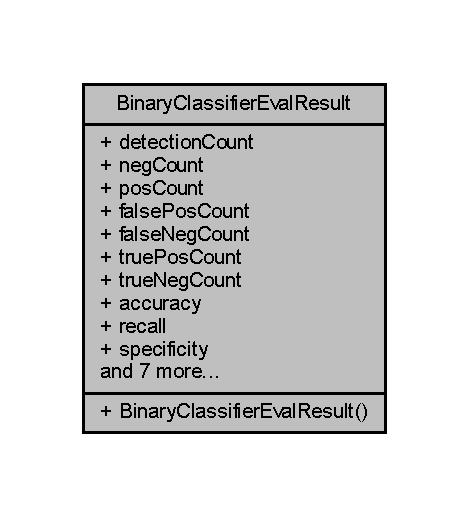
\includegraphics[width=225pt]{struct_vision_core_1_1_evaluation_1_1_binary_classifier_eval_result__coll__graph}
\end{center}
\end{figure}
\subsection*{Public Member Functions}
\begin{DoxyCompactItemize}
\item 
\hypertarget{struct_vision_core_1_1_evaluation_1_1_binary_classifier_eval_result_a56ffb62efd16fc45f18938e1fcdb2375}{}\hyperlink{struct_vision_core_1_1_evaluation_1_1_binary_classifier_eval_result_a56ffb62efd16fc45f18938e1fcdb2375}{Binary\+Classifier\+Eval\+Result} ()\label{struct_vision_core_1_1_evaluation_1_1_binary_classifier_eval_result_a56ffb62efd16fc45f18938e1fcdb2375}

\begin{DoxyCompactList}\small\item\em Default contructor. \end{DoxyCompactList}\end{DoxyCompactItemize}
\subsection*{Public Attributes}
\begin{DoxyCompactItemize}
\item 
\hypertarget{struct_vision_core_1_1_evaluation_1_1_binary_classifier_eval_result_a3106f64e0c19391502195e9d87ef882d}{}unsigned int \hyperlink{struct_vision_core_1_1_evaluation_1_1_binary_classifier_eval_result_a3106f64e0c19391502195e9d87ef882d}{detection\+Count}\label{struct_vision_core_1_1_evaluation_1_1_binary_classifier_eval_result_a3106f64e0c19391502195e9d87ef882d}

\begin{DoxyCompactList}\small\item\em Total number of tested instances. \end{DoxyCompactList}\item 
\hypertarget{struct_vision_core_1_1_evaluation_1_1_binary_classifier_eval_result_a2376a6d0e1290c06595de6d5de9cd7d2}{}unsigned int \hyperlink{struct_vision_core_1_1_evaluation_1_1_binary_classifier_eval_result_a2376a6d0e1290c06595de6d5de9cd7d2}{neg\+Count}\label{struct_vision_core_1_1_evaluation_1_1_binary_classifier_eval_result_a2376a6d0e1290c06595de6d5de9cd7d2}

\begin{DoxyCompactList}\small\item\em Number of negative instances. \end{DoxyCompactList}\item 
\hypertarget{struct_vision_core_1_1_evaluation_1_1_binary_classifier_eval_result_a4c917d6fa9d6dcd308a3b44f376a580e}{}unsigned int \hyperlink{struct_vision_core_1_1_evaluation_1_1_binary_classifier_eval_result_a4c917d6fa9d6dcd308a3b44f376a580e}{pos\+Count}\label{struct_vision_core_1_1_evaluation_1_1_binary_classifier_eval_result_a4c917d6fa9d6dcd308a3b44f376a580e}

\begin{DoxyCompactList}\small\item\em Number of positive instances. \end{DoxyCompactList}\item 
\hypertarget{struct_vision_core_1_1_evaluation_1_1_binary_classifier_eval_result_a37d9752b7bc1fe547579c3d34350d789}{}unsigned int \hyperlink{struct_vision_core_1_1_evaluation_1_1_binary_classifier_eval_result_a37d9752b7bc1fe547579c3d34350d789}{false\+Pos\+Count}\label{struct_vision_core_1_1_evaluation_1_1_binary_classifier_eval_result_a37d9752b7bc1fe547579c3d34350d789}

\begin{DoxyCompactList}\small\item\em Number of false positives. \end{DoxyCompactList}\item 
\hypertarget{struct_vision_core_1_1_evaluation_1_1_binary_classifier_eval_result_a3a724b2694d3cdc8174e9bf3980f6b6e}{}unsigned int \hyperlink{struct_vision_core_1_1_evaluation_1_1_binary_classifier_eval_result_a3a724b2694d3cdc8174e9bf3980f6b6e}{false\+Neg\+Count}\label{struct_vision_core_1_1_evaluation_1_1_binary_classifier_eval_result_a3a724b2694d3cdc8174e9bf3980f6b6e}

\begin{DoxyCompactList}\small\item\em Number of false negatives. \end{DoxyCompactList}\item 
\hypertarget{struct_vision_core_1_1_evaluation_1_1_binary_classifier_eval_result_ab14e03e0a494c8495d3cff1629fed7ca}{}unsigned int \hyperlink{struct_vision_core_1_1_evaluation_1_1_binary_classifier_eval_result_ab14e03e0a494c8495d3cff1629fed7ca}{true\+Pos\+Count}\label{struct_vision_core_1_1_evaluation_1_1_binary_classifier_eval_result_ab14e03e0a494c8495d3cff1629fed7ca}

\begin{DoxyCompactList}\small\item\em Number of true positives. \end{DoxyCompactList}\item 
\hypertarget{struct_vision_core_1_1_evaluation_1_1_binary_classifier_eval_result_a7b82bda4b18441fe2758efc93fb66cc3}{}unsigned int \hyperlink{struct_vision_core_1_1_evaluation_1_1_binary_classifier_eval_result_a7b82bda4b18441fe2758efc93fb66cc3}{true\+Neg\+Count}\label{struct_vision_core_1_1_evaluation_1_1_binary_classifier_eval_result_a7b82bda4b18441fe2758efc93fb66cc3}

\begin{DoxyCompactList}\small\item\em Number of true negatives. \end{DoxyCompactList}\item 
\hypertarget{struct_vision_core_1_1_evaluation_1_1_binary_classifier_eval_result_a6e55b938786bd86846860397d25c10bd}{}double \hyperlink{struct_vision_core_1_1_evaluation_1_1_binary_classifier_eval_result_a6e55b938786bd86846860397d25c10bd}{accuracy}\label{struct_vision_core_1_1_evaluation_1_1_binary_classifier_eval_result_a6e55b938786bd86846860397d25c10bd}

\begin{DoxyCompactList}\small\item\em Accuracy ~\newline
 $ ACC = \frac{TP+TN}{P+N} $. \end{DoxyCompactList}\item 
\hypertarget{struct_vision_core_1_1_evaluation_1_1_binary_classifier_eval_result_a0fb25e19c2b2cfc018d2ef6cdf7947e3}{}double \hyperlink{struct_vision_core_1_1_evaluation_1_1_binary_classifier_eval_result_a0fb25e19c2b2cfc018d2ef6cdf7947e3}{recall}\label{struct_vision_core_1_1_evaluation_1_1_binary_classifier_eval_result_a0fb25e19c2b2cfc018d2ef6cdf7947e3}

\begin{DoxyCompactList}\small\item\em Recall (Sensitivity/ Hit Rate) ~\newline
 $ TPR = \frac{TP}{P} $. \end{DoxyCompactList}\item 
\hypertarget{struct_vision_core_1_1_evaluation_1_1_binary_classifier_eval_result_aad6585357e6c67247c6fefc19d496272}{}double \hyperlink{struct_vision_core_1_1_evaluation_1_1_binary_classifier_eval_result_aad6585357e6c67247c6fefc19d496272}{specificity}\label{struct_vision_core_1_1_evaluation_1_1_binary_classifier_eval_result_aad6585357e6c67247c6fefc19d496272}

\begin{DoxyCompactList}\small\item\em Specificity ~\newline
 $ SPC = \frac{TN}{N} $. \end{DoxyCompactList}\item 
\hypertarget{struct_vision_core_1_1_evaluation_1_1_binary_classifier_eval_result_a98ce42142601aa81694132ce8af84e8b}{}double \hyperlink{struct_vision_core_1_1_evaluation_1_1_binary_classifier_eval_result_a98ce42142601aa81694132ce8af84e8b}{precision}\label{struct_vision_core_1_1_evaluation_1_1_binary_classifier_eval_result_a98ce42142601aa81694132ce8af84e8b}

\begin{DoxyCompactList}\small\item\em Precision or positive predictive value (correct detections) ~\newline
 $ PPV = \frac{TP}{TP+FP} $. \end{DoxyCompactList}\item 
\hypertarget{struct_vision_core_1_1_evaluation_1_1_binary_classifier_eval_result_a2f35bc80bfff53daa8746f9b7cbcb3a2}{}double \hyperlink{struct_vision_core_1_1_evaluation_1_1_binary_classifier_eval_result_a2f35bc80bfff53daa8746f9b7cbcb3a2}{npv}\label{struct_vision_core_1_1_evaluation_1_1_binary_classifier_eval_result_a2f35bc80bfff53daa8746f9b7cbcb3a2}

\begin{DoxyCompactList}\small\item\em Negative predictive value (the percent of negatives that are correctly classified) ~\newline
 $ NPV = \frac{TN}{TN+FN} $. \end{DoxyCompactList}\item 
\hypertarget{struct_vision_core_1_1_evaluation_1_1_binary_classifier_eval_result_abc38975fd884497b24f52b828cec9f1b}{}double \hyperlink{struct_vision_core_1_1_evaluation_1_1_binary_classifier_eval_result_abc38975fd884497b24f52b828cec9f1b}{fallout}\label{struct_vision_core_1_1_evaluation_1_1_binary_classifier_eval_result_abc38975fd884497b24f52b828cec9f1b}

\begin{DoxyCompactList}\small\item\em Fall-\/out or false positive rate ~\newline
 $ FPR = \frac{FP}{N} $. \end{DoxyCompactList}\item 
\hypertarget{struct_vision_core_1_1_evaluation_1_1_binary_classifier_eval_result_a4b55320813a56a9e113b23525e17f574}{}double \hyperlink{struct_vision_core_1_1_evaluation_1_1_binary_classifier_eval_result_a4b55320813a56a9e113b23525e17f574}{fdr}\label{struct_vision_core_1_1_evaluation_1_1_binary_classifier_eval_result_a4b55320813a56a9e113b23525e17f574}

\begin{DoxyCompactList}\small\item\em False discovery rate ~\newline
 $ FDR = \frac{FP}{FP+TP} $. \end{DoxyCompactList}\item 
\hypertarget{struct_vision_core_1_1_evaluation_1_1_binary_classifier_eval_result_a2f9dbff026930716e4e219ce2d94b6f1}{}double \hyperlink{struct_vision_core_1_1_evaluation_1_1_binary_classifier_eval_result_a2f9dbff026930716e4e219ce2d94b6f1}{fnr}\label{struct_vision_core_1_1_evaluation_1_1_binary_classifier_eval_result_a2f9dbff026930716e4e219ce2d94b6f1}

\begin{DoxyCompactList}\small\item\em False negative rate ~\newline
 $ FNR = \frac{FN}{FN + TP} $. \end{DoxyCompactList}\item 
\hypertarget{struct_vision_core_1_1_evaluation_1_1_binary_classifier_eval_result_a71afe1789388eaf7cf65d0de39800e5d}{}double \hyperlink{struct_vision_core_1_1_evaluation_1_1_binary_classifier_eval_result_a71afe1789388eaf7cf65d0de39800e5d}{mcc}\label{struct_vision_core_1_1_evaluation_1_1_binary_classifier_eval_result_a71afe1789388eaf7cf65d0de39800e5d}

\begin{DoxyCompactList}\small\item\em Matthews correlation coefficient is used in machine learning as a measure of the quality of binary (two-\/class) classifications. ~\newline
 $ MCC = \frac{TP \times TN - FP \times FN}{\sqrt{(TP+FP)(TP+FN)(TN+FP)(TN+FN)}} $. \end{DoxyCompactList}\item 
\hypertarget{struct_vision_core_1_1_evaluation_1_1_binary_classifier_eval_result_ac8bfb2aa00ec18131ea1b1f9383a8c8f}{}double \hyperlink{struct_vision_core_1_1_evaluation_1_1_binary_classifier_eval_result_ac8bfb2aa00ec18131ea1b1f9383a8c8f}{f1score}\label{struct_vision_core_1_1_evaluation_1_1_binary_classifier_eval_result_ac8bfb2aa00ec18131ea1b1f9383a8c8f}

\begin{DoxyCompactList}\small\item\em F1 score (is the harmonic mean of precision and recall) ~\newline
 $ F_{1} = \frac{2 \times PPV \times TPR}{PPV + TPR} $. \end{DoxyCompactList}\end{DoxyCompactItemize}


\subsection{Detailed Description}
Data structure that stores the statistics and evaluation data for a binary classifier. 

\begin{DoxySeeAlso}{See also}
\hyperlink{class_vision_core_1_1_evaluation_1_1_binary_classifier_evaluator}{Binary\+Classifier\+Evaluator} 
\end{DoxySeeAlso}


Definition at line 779 of file Vision\+Evaluation.\+h.



The documentation for this struct was generated from the following file\+:\begin{DoxyCompactItemize}
\item 
D\+:/\+F\+U\+R\+G/\+Software/\+Cv\+Works\+Release1/\+Core/\+Vision/Vision\+Evaluation.\+h\end{DoxyCompactItemize}

\hypertarget{class_vision_core_1_1_evaluation_1_1_binary_classifier_evaluator}{}\section{Binary\+Classifier\+Evaluator Class Reference}
\label{class_vision_core_1_1_evaluation_1_1_binary_classifier_evaluator}\index{Binary\+Classifier\+Evaluator@{Binary\+Classifier\+Evaluator}}


{\ttfamily \#include $<$Vision\+Evaluation.\+h$>$}



Collaboration diagram for Binary\+Classifier\+Evaluator\+:
\nopagebreak
\begin{figure}[H]
\begin{center}
\leavevmode
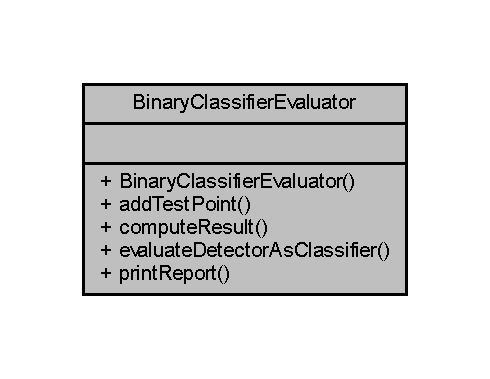
\includegraphics[width=235pt]{class_vision_core_1_1_evaluation_1_1_binary_classifier_evaluator__coll__graph}
\end{center}
\end{figure}
\subsection*{Public Member Functions}
\begin{DoxyCompactItemize}
\item 
\hypertarget{class_vision_core_1_1_evaluation_1_1_binary_classifier_evaluator_ac752f3567078dfabdfcaf82b272f3040}{}\hyperlink{class_vision_core_1_1_evaluation_1_1_binary_classifier_evaluator_ac752f3567078dfabdfcaf82b272f3040}{Binary\+Classifier\+Evaluator} ()\label{class_vision_core_1_1_evaluation_1_1_binary_classifier_evaluator_ac752f3567078dfabdfcaf82b272f3040}

\begin{DoxyCompactList}\small\item\em Default Constuctor. \end{DoxyCompactList}\item 
\hypertarget{class_vision_core_1_1_evaluation_1_1_binary_classifier_evaluator_af2197d681f638fd535e08c3cc559254a}{}void \hyperlink{class_vision_core_1_1_evaluation_1_1_binary_classifier_evaluator_af2197d681f638fd535e08c3cc559254a}{add\+Test\+Point} (bool det\+Result, bool ground\+Truth)\label{class_vision_core_1_1_evaluation_1_1_binary_classifier_evaluator_af2197d681f638fd535e08c3cc559254a}

\begin{DoxyCompactList}\small\item\em Add a detection -\/ ground truth pair. \end{DoxyCompactList}\item 
\hyperlink{struct_vision_core_1_1_evaluation_1_1_binary_classifier_eval_result}{Binary\+Classifier\+Eval\+Result} \hyperlink{class_vision_core_1_1_evaluation_1_1_binary_classifier_evaluator_ad578be8e9cf0140bf74635da8e5345d4}{compute\+Result} ()
\begin{DoxyCompactList}\small\item\em Compute the results using the data provided via \textquotesingle{}add\+Test\+Point\textquotesingle{}. \end{DoxyCompactList}\item 
{\footnotesize template$<$class T\+Img , class T\+Obj1 , class T\+Obj2 $>$ }\\\hyperlink{struct_vision_core_1_1_evaluation_1_1_binary_classifier_eval_result}{Binary\+Classifier\+Eval\+Result} \hyperlink{class_vision_core_1_1_evaluation_1_1_binary_classifier_evaluator_a40a3e0ed913bf943beefc171ed0162d3}{evaluate\+Detector\+As\+Classifier} (const \hyperlink{class_vision_core_1_1_interfaces_1_1_detector}{Detector}$<$ T\+Img, T\+Obj1 $>$ \&det, \hyperlink{class_vision_core_1_1_evaluation_1_1_detection_dataset}{Detection\+Dataset}$<$ T\+Img, T\+Obj2 $>$ \&dataset)
\begin{DoxyCompactList}\small\item\em Helper function that iterates over a dataset by calling the detector for each image and comparing the result with the ground truth. By default, if a image has groundtruth annotations it is considered as a positive instance. Elsewhere, it is considered as a negative instance. \end{DoxyCompactList}\end{DoxyCompactItemize}
\subsection*{Static Public Member Functions}
\begin{DoxyCompactItemize}
\item 
\hypertarget{class_vision_core_1_1_evaluation_1_1_binary_classifier_evaluator_a54604d384e1a55cb93b04a640179eac0}{}static void \hyperlink{class_vision_core_1_1_evaluation_1_1_binary_classifier_evaluator_a54604d384e1a55cb93b04a640179eac0}{print\+Report} (const \hyperlink{struct_vision_core_1_1_evaluation_1_1_binary_classifier_eval_result}{Binary\+Classifier\+Eval\+Result} \&result, std\+::ostream \&out=std\+::cout)\label{class_vision_core_1_1_evaluation_1_1_binary_classifier_evaluator_a54604d384e1a55cb93b04a640179eac0}

\begin{DoxyCompactList}\small\item\em Print the report for a binary classifier evaluation. By default recall and precision metrics are given considering the \textquotesingle{}true\textquotesingle{} samples. \end{DoxyCompactList}\end{DoxyCompactItemize}


\subsection{Detailed Description}
Class that performs a binary classifier evaluation. There are two different ways to perform a evaluation of a binary classifier (or a detector as a classifier)\+:

1) Manual\+: For each image in the test set, run the detector/classifier and use the detector $<$stront$>$output + grountruth$<$/stron$>$ as input for the add\+Test\+Point. A Test\+Point is usually one frame. You have to convert the output to boolean. To compute the evaluation results use the funcion \textquotesingle{}compute\+Results\textquotesingle{}. To print the output use the \textquotesingle{}print\+Report\textquotesingle{} function.

2) Auto\+: Using the \textquotesingle{}evaluate\+Detector\+As\+Classifier\textquotesingle{} function to perform a evaluation of the whole dataset (\hyperlink{class_vision_core_1_1_evaluation_1_1_detection_dataset}{Detection\+Dataset} class). The method will assume that a empty vector is a negative and any non-\/empty vector is a positive. It executes all the steps above. 

Definition at line 876 of file Vision\+Evaluation.\+h.



\subsection{Member Function Documentation}
\hypertarget{class_vision_core_1_1_evaluation_1_1_binary_classifier_evaluator_ad578be8e9cf0140bf74635da8e5345d4}{}\index{Vision\+Core\+::\+Evaluation\+::\+Binary\+Classifier\+Evaluator@{Vision\+Core\+::\+Evaluation\+::\+Binary\+Classifier\+Evaluator}!compute\+Result@{compute\+Result}}
\index{compute\+Result@{compute\+Result}!Vision\+Core\+::\+Evaluation\+::\+Binary\+Classifier\+Evaluator@{Vision\+Core\+::\+Evaluation\+::\+Binary\+Classifier\+Evaluator}}
\subsubsection[{compute\+Result()}]{\setlength{\rightskip}{0pt plus 5cm}{\bf Binary\+Classifier\+Eval\+Result} compute\+Result (
\begin{DoxyParamCaption}
{}
\end{DoxyParamCaption}
)\hspace{0.3cm}{\ttfamily [inline]}}\label{class_vision_core_1_1_evaluation_1_1_binary_classifier_evaluator_ad578be8e9cf0140bf74635da8e5345d4}


Compute the results using the data provided via \textquotesingle{}add\+Test\+Point\textquotesingle{}. 

Computed statistics\+: Accuracy ~\newline
 $ ACC = \frac{TP+TN}{P+N} $

Recall (Sensitivity/ Hit Rate) ~\newline
 $ TPR = \frac{TP}{P} $

Specificity ~\newline
 $ SPC = \frac{TN}{N} $

Precision or positive predictive value (correct detections) ~\newline
 $ PPV = \frac{TP}{TP+FP} $

Negative predictive value (the percent of negatives that are correctly classified) ~\newline
 $ NPV = \frac{TN}{TN+FN} $

Fall-\/out or false positive rate ~\newline
 $ FPR = \frac{FP}{N} $

False discovery rate ~\newline
 $ FDR = \frac{FP}{FP+TP} $

False negative rate ~\newline
 $ FNR = \frac{FN}{FN + TP} $

Matthews correlation coefficient is used in machine learning as a measure of the quality of binary (two-\/class) classifications. ~\newline
 $ MCC = \frac{TP \times TN - FP \times FN}{\sqrt{(TP+FP)(TP+FN)(TN+FP)(TN+FN)}} $

F1 score (is the harmonic mean of precision and recall) ~\newline
 $ F_{1} = \frac{2 \times PPV \times TPR}{PPV + TPR} $ 

Definition at line 898 of file Vision\+Evaluation.\+h.



Here is the caller graph for this function\+:
\nopagebreak
\begin{figure}[H]
\begin{center}
\leavevmode
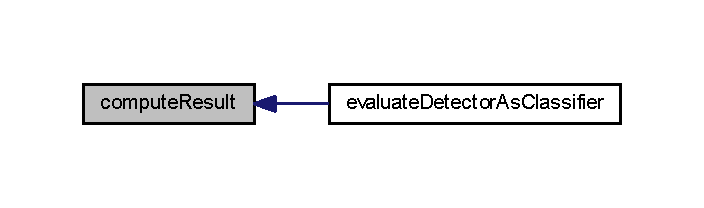
\includegraphics[width=338pt]{class_vision_core_1_1_evaluation_1_1_binary_classifier_evaluator_ad578be8e9cf0140bf74635da8e5345d4_icgraph}
\end{center}
\end{figure}


\hypertarget{class_vision_core_1_1_evaluation_1_1_binary_classifier_evaluator_a40a3e0ed913bf943beefc171ed0162d3}{}\index{Vision\+Core\+::\+Evaluation\+::\+Binary\+Classifier\+Evaluator@{Vision\+Core\+::\+Evaluation\+::\+Binary\+Classifier\+Evaluator}!evaluate\+Detector\+As\+Classifier@{evaluate\+Detector\+As\+Classifier}}
\index{evaluate\+Detector\+As\+Classifier@{evaluate\+Detector\+As\+Classifier}!Vision\+Core\+::\+Evaluation\+::\+Binary\+Classifier\+Evaluator@{Vision\+Core\+::\+Evaluation\+::\+Binary\+Classifier\+Evaluator}}
\subsubsection[{evaluate\+Detector\+As\+Classifier(const Detector$<$ T\+Img, T\+Obj1 $>$ \&det, Detection\+Dataset$<$ T\+Img, T\+Obj2 $>$ \&dataset)}]{\setlength{\rightskip}{0pt plus 5cm}{\bf Binary\+Classifier\+Eval\+Result} evaluate\+Detector\+As\+Classifier (
\begin{DoxyParamCaption}
\item[{const {\bf Detector}$<$ T\+Img, T\+Obj1 $>$ \&}]{det, }
\item[{{\bf Detection\+Dataset}$<$ T\+Img, T\+Obj2 $>$ \&}]{dataset}
\end{DoxyParamCaption}
)\hspace{0.3cm}{\ttfamily [inline]}}\label{class_vision_core_1_1_evaluation_1_1_binary_classifier_evaluator_a40a3e0ed913bf943beefc171ed0162d3}


Helper function that iterates over a dataset by calling the detector for each image and comparing the result with the ground truth. By default, if a image has groundtruth annotations it is considered as a positive instance. Elsewhere, it is considered as a negative instance. 


\begin{DoxyParams}{Parameters}
{\em T\+Img} & Tipo de imagem. \\
\hline
{\em T\+Obj1} & Detector output object type. \\
\hline
{\em T\+Obj2} & Ground truth annotation object type \\
\hline
\end{DoxyParams}


Definition at line 1003 of file Vision\+Evaluation.\+h.



Here is the call graph for this function\+:
\nopagebreak
\begin{figure}[H]
\begin{center}
\leavevmode
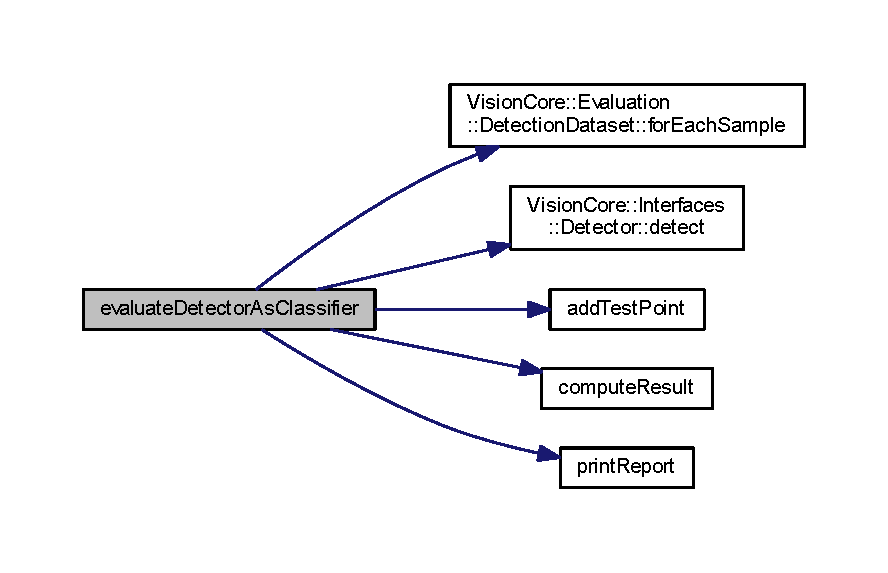
\includegraphics[width=350pt]{class_vision_core_1_1_evaluation_1_1_binary_classifier_evaluator_a40a3e0ed913bf943beefc171ed0162d3_cgraph}
\end{center}
\end{figure}




The documentation for this class was generated from the following file\+:\begin{DoxyCompactItemize}
\item 
D\+:/\+F\+U\+R\+G/\+Software/\+Cv\+Works\+Release1/\+Core/\+Vision/Vision\+Evaluation.\+h\end{DoxyCompactItemize}

\hypertarget{class_vision_core_1_1_interfaces_1_1_categorizer}{}\section{Categorizer$<$ T\+In, T\+Ctg $>$ Class Template Reference}
\label{class_vision_core_1_1_interfaces_1_1_categorizer}\index{Categorizer$<$ T\+In, T\+Ctg $>$@{Categorizer$<$ T\+In, T\+Ctg $>$}}


Interface defining a generic image categorizer (classifier).  




{\ttfamily \#include $<$Vision\+Interfaces.\+h$>$}



Collaboration diagram for Categorizer$<$ T\+In, T\+Ctg $>$\+:
\nopagebreak
\begin{figure}[H]
\begin{center}
\leavevmode
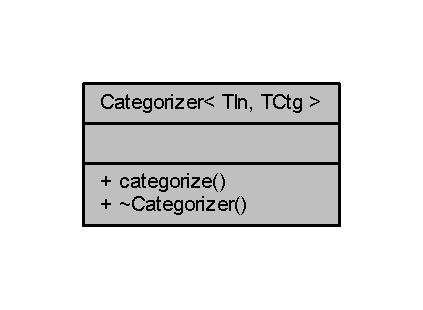
\includegraphics[width=203pt]{class_vision_core_1_1_interfaces_1_1_categorizer__coll__graph}
\end{center}
\end{figure}
\subsection*{Public Types}
\begin{DoxyCompactItemize}
\item 
\hypertarget{class_vision_core_1_1_interfaces_1_1_categorizer_af1a26d383531f9b1b26326efb2790721}{}typedef T\+In {\bfseries In\+Type}\label{class_vision_core_1_1_interfaces_1_1_categorizer_af1a26d383531f9b1b26326efb2790721}

\item 
\hypertarget{class_vision_core_1_1_interfaces_1_1_categorizer_a502f5b85c2a6367e444122eb8878de94}{}typedef T\+Ctg {\bfseries Ctg\+Type}\label{class_vision_core_1_1_interfaces_1_1_categorizer_a502f5b85c2a6367e444122eb8878de94}

\end{DoxyCompactItemize}
\subsection*{Public Member Functions}
\begin{DoxyCompactItemize}
\item 
\hypertarget{class_vision_core_1_1_interfaces_1_1_categorizer_a84db45703ada48a63144e69f63e73bf5}{}virtual T\+Ctg \hyperlink{class_vision_core_1_1_interfaces_1_1_categorizer_a84db45703ada48a63144e69f63e73bf5}{categorize} (const T\+In \&sample) const  =0\label{class_vision_core_1_1_interfaces_1_1_categorizer_a84db45703ada48a63144e69f63e73bf5}

\begin{DoxyCompactList}\small\item\em Process an input sample and outputs its category. \end{DoxyCompactList}\item 
\hypertarget{class_vision_core_1_1_interfaces_1_1_categorizer_ab8cf3f49e6c511eeccc1d17befdcaf46}{}virtual \hyperlink{class_vision_core_1_1_interfaces_1_1_categorizer_ab8cf3f49e6c511eeccc1d17befdcaf46}{$\sim$\+Categorizer} ()\label{class_vision_core_1_1_interfaces_1_1_categorizer_ab8cf3f49e6c511eeccc1d17befdcaf46}

\begin{DoxyCompactList}\small\item\em Destructor. \end{DoxyCompactList}\end{DoxyCompactItemize}


\subsection{Detailed Description}
\subsubsection*{template$<$class T\+In, typename T\+Ctg = std\+::string$>$class Vision\+Core\+::\+Interfaces\+::\+Categorizer$<$ T\+In, T\+Ctg $>$}

Interface defining a generic image categorizer (classifier). 

A image categorizer (or classifier) is capeable of identifing the category of a given image.

For example, a binary classifier could be able to classify an image as being a forest or city.

The interface defines only one method\+: \hyperlink{class_vision_core_1_1_interfaces_1_1_categorizer_a84db45703ada48a63144e69f63e73bf5}{categorize()}, which receives an input image and returns the category. The default category type is std\+::string, but it can be specifyied (for example as bool for binary classifiers).


\begin{DoxyParams}{Parameters}
{\em T\+In} & Image type. \\
\hline
{\em T\+Obj} & Category type. Default is std\+::string. \\
\hline
\end{DoxyParams}


Definition at line 252 of file Vision\+Interfaces.\+h.



The documentation for this class was generated from the following file\+:\begin{DoxyCompactItemize}
\item 
D\+:/\+F\+U\+R\+G/\+Software/\+Cv\+Works\+Release1/\+Core/\+Vision/Vision\+Interfaces.\+h\end{DoxyCompactItemize}

\hypertarget{class_viscv_1_1_circle}{}\section{Circle$<$ T $>$ Class Template Reference}
\label{class_viscv_1_1_circle}\index{Circle$<$ T $>$@{Circle$<$ T $>$}}


Defines a circle. Stores the center (x,y) and radius.  




{\ttfamily \#include $<$Circle\+Detector\+H\+T\+C\+F.\+h$>$}



Collaboration diagram for Circle$<$ T $>$\+:
\nopagebreak
\begin{figure}[H]
\begin{center}
\leavevmode
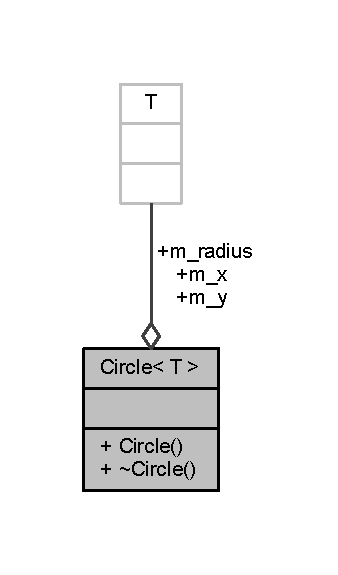
\includegraphics[width=162pt]{class_viscv_1_1_circle__coll__graph}
\end{center}
\end{figure}
\subsection*{Public Member Functions}
\begin{DoxyCompactItemize}
\item 
\hypertarget{class_viscv_1_1_circle_a08855c3fd479dc105858c8283c32d190}{}\hyperlink{class_viscv_1_1_circle_a08855c3fd479dc105858c8283c32d190}{Circle} (T x, T y, T radius)\label{class_viscv_1_1_circle_a08855c3fd479dc105858c8283c32d190}

\begin{DoxyCompactList}\small\item\em Constructor method. \end{DoxyCompactList}\item 
\hypertarget{class_viscv_1_1_circle_a2517abc7a8f9949c93453562e309cf0e}{}virtual \hyperlink{class_viscv_1_1_circle_a2517abc7a8f9949c93453562e309cf0e}{$\sim$\+Circle} ()\label{class_viscv_1_1_circle_a2517abc7a8f9949c93453562e309cf0e}

\begin{DoxyCompactList}\small\item\em Destructor method. \end{DoxyCompactList}\end{DoxyCompactItemize}
\subsection*{Public Attributes}
\begin{DoxyCompactItemize}
\item 
\hypertarget{class_viscv_1_1_circle_ae356e3ca959691f5bc00088864a6e6cb}{}T {\bfseries m\+\_\+radius}\label{class_viscv_1_1_circle_ae356e3ca959691f5bc00088864a6e6cb}

\item 
\hypertarget{class_viscv_1_1_circle_af0fee1836830b9855a6a29266b2131cd}{}T {\bfseries m\+\_\+x}\label{class_viscv_1_1_circle_af0fee1836830b9855a6a29266b2131cd}

\item 
\hypertarget{class_viscv_1_1_circle_acf382cd74d7b11876e21cffd842333f0}{}T {\bfseries m\+\_\+y}\label{class_viscv_1_1_circle_acf382cd74d7b11876e21cffd842333f0}

\end{DoxyCompactItemize}


\subsection{Detailed Description}
\subsubsection*{template$<$typename T = int$>$class Viscv\+::\+Circle$<$ T $>$}

Defines a circle. Stores the center (x,y) and radius. 

Definition at line 36 of file Circle\+Detector\+H\+T\+C\+F.\+h.



The documentation for this class was generated from the following file\+:\begin{DoxyCompactItemize}
\item 
D\+:/\+F\+U\+R\+G/\+Software/\+Cv\+Works\+Release1/\+Components/\+Vision\+Implementation\+Cv/Circle\+Detector\+H\+T\+C\+F.\+h\end{DoxyCompactItemize}

\hypertarget{class_viscv_1_1_circle_detector_h_t_c_f}{}\section{Circle\+Detector\+H\+T\+C\+F Class Reference}
\label{class_viscv_1_1_circle_detector_h_t_c_f}\index{Circle\+Detector\+H\+T\+C\+F@{Circle\+Detector\+H\+T\+C\+F}}


Detects circles using Hough Transform and (optionally) Color Filter (H\+T\+C\+F).  




{\ttfamily \#include $<$Circle\+Detector\+H\+T\+C\+F.\+h$>$}



Inheritance diagram for Circle\+Detector\+H\+T\+C\+F\+:
\nopagebreak
\begin{figure}[H]
\begin{center}
\leavevmode
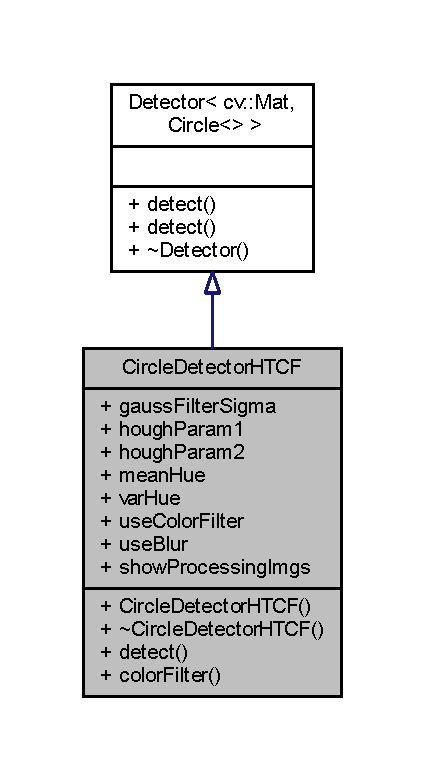
\includegraphics[width=204pt]{class_viscv_1_1_circle_detector_h_t_c_f__inherit__graph}
\end{center}
\end{figure}


Collaboration diagram for Circle\+Detector\+H\+T\+C\+F\+:
\nopagebreak
\begin{figure}[H]
\begin{center}
\leavevmode
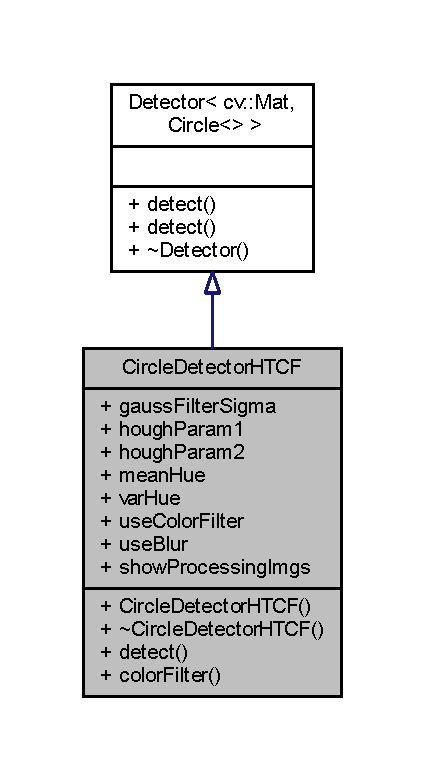
\includegraphics[width=204pt]{class_viscv_1_1_circle_detector_h_t_c_f__coll__graph}
\end{center}
\end{figure}
\subsection*{Public Member Functions}
\begin{DoxyCompactItemize}
\item 
\hypertarget{class_viscv_1_1_circle_detector_h_t_c_f_a8eb782145f34bac05e1ba977e791caf8}{}\hyperlink{class_viscv_1_1_circle_detector_h_t_c_f_a8eb782145f34bac05e1ba977e791caf8}{Circle\+Detector\+H\+T\+C\+F} ()\label{class_viscv_1_1_circle_detector_h_t_c_f_a8eb782145f34bac05e1ba977e791caf8}

\begin{DoxyCompactList}\small\item\em Constructor method. \end{DoxyCompactList}\item 
\hypertarget{class_viscv_1_1_circle_detector_h_t_c_f_a036330f1968940ca58930329dd66f05b}{}virtual \hyperlink{class_viscv_1_1_circle_detector_h_t_c_f_a036330f1968940ca58930329dd66f05b}{$\sim$\+Circle\+Detector\+H\+T\+C\+F} ()\label{class_viscv_1_1_circle_detector_h_t_c_f_a036330f1968940ca58930329dd66f05b}

\begin{DoxyCompactList}\small\item\em Destructor method. \end{DoxyCompactList}\item 
std\+::vector$<$ \hyperlink{class_viscv_1_1_circle}{Circle}$<$$>$ $>$ \hyperlink{class_viscv_1_1_circle_detector_h_t_c_f_ad8f008988f0c246f86a192f8c17c3a88}{detect} (const cv\+::\+Mat \&img) const 
\begin{DoxyCompactList}\small\item\em Detects objects in the image and returns a vector with the detected objects. \end{DoxyCompactList}\item 
\hypertarget{class_viscv_1_1_circle_detector_h_t_c_f_ad4da52b5daa1da09a46aa725cde4bb93}{}void \hyperlink{class_viscv_1_1_circle_detector_h_t_c_f_ad4da52b5daa1da09a46aa725cde4bb93}{color\+Filter} (const cv\+::\+Mat \&src, cv\+::\+Mat \&dst) const \label{class_viscv_1_1_circle_detector_h_t_c_f_ad4da52b5daa1da09a46aa725cde4bb93}

\begin{DoxyCompactList}\small\item\em Computa uma imagem contendo somente os pixels com hue entre os limites especificados em mean\+Hue e var\+Hue. \end{DoxyCompactList}\end{DoxyCompactItemize}
\subsection*{Public Attributes}
\begin{DoxyCompactItemize}
\item 
double \hyperlink{class_viscv_1_1_circle_detector_h_t_c_f_ad834b1ab28e93958d183da062dbcbe42}{gauss\+Filter\+Sigma}
\begin{DoxyCompactList}\small\item\em Desvio padrão do filtro Gaussiano (relativo ao número de linhas da imagem) \end{DoxyCompactList}\item 
\hypertarget{class_viscv_1_1_circle_detector_h_t_c_f_a001ce4c829b6bfed69328dde68c616aa}{}double \hyperlink{class_viscv_1_1_circle_detector_h_t_c_f_a001ce4c829b6bfed69328dde68c616aa}{hough\+Param1}\label{class_viscv_1_1_circle_detector_h_t_c_f_a001ce4c829b6bfed69328dde68c616aa}

\begin{DoxyCompactList}\small\item\em Parametro 1 da transformada de Hough na Open\+Cv. \end{DoxyCompactList}\item 
\hypertarget{class_viscv_1_1_circle_detector_h_t_c_f_ab33e718b70d4cbd105ad85370ce6f6c4}{}double \hyperlink{class_viscv_1_1_circle_detector_h_t_c_f_ab33e718b70d4cbd105ad85370ce6f6c4}{hough\+Param2}\label{class_viscv_1_1_circle_detector_h_t_c_f_ab33e718b70d4cbd105ad85370ce6f6c4}

\begin{DoxyCompactList}\small\item\em Parametro 2 da transformada de Hough na Open\+Cv. \end{DoxyCompactList}\item 
\hypertarget{class_viscv_1_1_circle_detector_h_t_c_f_a8d3181a667ab3c5a95bafdb5b40abb91}{}int \hyperlink{class_viscv_1_1_circle_detector_h_t_c_f_a8d3181a667ab3c5a95bafdb5b40abb91}{mean\+Hue}\label{class_viscv_1_1_circle_detector_h_t_c_f_a8d3181a667ab3c5a95bafdb5b40abb91}

\begin{DoxyCompactList}\small\item\em Hue médio do filtro de cor \mbox{[}0,179\mbox{]}. \end{DoxyCompactList}\item 
int \hyperlink{class_viscv_1_1_circle_detector_h_t_c_f_a4b6c2bf89ae1855a664ac3d25a60f71e}{var\+Hue}
\begin{DoxyCompactList}\small\item\em Variância (tolerância) do filtro de cor \mbox{[}0,90\mbox{]}. \end{DoxyCompactList}\item 
\hypertarget{class_viscv_1_1_circle_detector_h_t_c_f_ae0ad1d0e8391baa5735df28c7a180328}{}bool \hyperlink{class_viscv_1_1_circle_detector_h_t_c_f_ae0ad1d0e8391baa5735df28c7a180328}{use\+Color\+Filter}\label{class_viscv_1_1_circle_detector_h_t_c_f_ae0ad1d0e8391baa5735df28c7a180328}

\begin{DoxyCompactList}\small\item\em Define se o filtro de cor deve ser utilizado ou não. \end{DoxyCompactList}\item 
\hypertarget{class_viscv_1_1_circle_detector_h_t_c_f_aa04568497fd0fc771dc37f6ad1450618}{}bool \hyperlink{class_viscv_1_1_circle_detector_h_t_c_f_aa04568497fd0fc771dc37f6ad1450618}{use\+Blur}\label{class_viscv_1_1_circle_detector_h_t_c_f_aa04568497fd0fc771dc37f6ad1450618}

\begin{DoxyCompactList}\small\item\em Define se o filtro gaussiano (blur) deve ser utilizado ou não. \end{DoxyCompactList}\item 
\hypertarget{class_viscv_1_1_circle_detector_h_t_c_f_ad56f3dc42f92c3f920caed1aec8ead03}{}bool \hyperlink{class_viscv_1_1_circle_detector_h_t_c_f_ad56f3dc42f92c3f920caed1aec8ead03}{show\+Processing\+Imgs}\label{class_viscv_1_1_circle_detector_h_t_c_f_ad56f3dc42f92c3f920caed1aec8ead03}

\begin{DoxyCompactList}\small\item\em Define se as imagens intermediárias de processamento devem ser mostradas. \end{DoxyCompactList}\end{DoxyCompactItemize}
\subsection*{Additional Inherited Members}


\subsection{Detailed Description}
Detects circles using Hough Transform and (optionally) Color Filter (H\+T\+C\+F). \begin{Desc}
\item[Examples\+: ]\par
\hyperlink{_vision_tests_2main_8cpp-example}{Vision\+Tests/main.\+cpp}.\end{Desc}


Definition at line 57 of file Circle\+Detector\+H\+T\+C\+F.\+h.



\subsection{Member Function Documentation}
\hypertarget{class_viscv_1_1_circle_detector_h_t_c_f_ad8f008988f0c246f86a192f8c17c3a88}{}\index{Viscv\+::\+Circle\+Detector\+H\+T\+C\+F@{Viscv\+::\+Circle\+Detector\+H\+T\+C\+F}!detect@{detect}}
\index{detect@{detect}!Viscv\+::\+Circle\+Detector\+H\+T\+C\+F@{Viscv\+::\+Circle\+Detector\+H\+T\+C\+F}}
\subsubsection[{detect(const cv\+::\+Mat \&img) const }]{\setlength{\rightskip}{0pt plus 5cm}std\+::vector$<$ {\bf Circle}$<$$>$ $>$ detect (
\begin{DoxyParamCaption}
\item[{const cv\+::\+Mat \&}]{img}
\end{DoxyParamCaption}
) const\hspace{0.3cm}{\ttfamily [virtual]}}\label{class_viscv_1_1_circle_detector_h_t_c_f_ad8f008988f0c246f86a192f8c17c3a88}


Detects objects in the image and returns a vector with the detected objects. 

The vector should be empty if no object is detected. 

Implements \hyperlink{class_vision_core_1_1_interfaces_1_1_detector_a0977745b253f810bb2ec009844618305}{Detector$<$ cv\+::\+Mat, Circle$<$$>$ $>$}.

\begin{Desc}
\item[Examples\+: ]\par
\hyperlink{_vision_tests_2main_8cpp-example}{Vision\+Tests/main.\+cpp}.\end{Desc}


Definition at line 76 of file Circle\+Detector\+H\+T\+C\+F.\+cpp.



Here is the call graph for this function\+:
\nopagebreak
\begin{figure}[H]
\begin{center}
\leavevmode
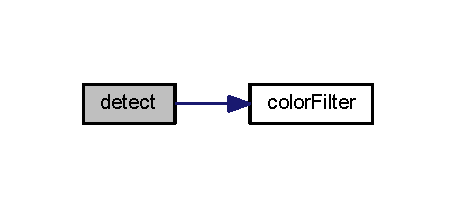
\includegraphics[width=219pt]{class_viscv_1_1_circle_detector_h_t_c_f_ad8f008988f0c246f86a192f8c17c3a88_cgraph}
\end{center}
\end{figure}




\subsection{Member Data Documentation}
\hypertarget{class_viscv_1_1_circle_detector_h_t_c_f_ad834b1ab28e93958d183da062dbcbe42}{}\index{Viscv\+::\+Circle\+Detector\+H\+T\+C\+F@{Viscv\+::\+Circle\+Detector\+H\+T\+C\+F}!gauss\+Filter\+Sigma@{gauss\+Filter\+Sigma}}
\index{gauss\+Filter\+Sigma@{gauss\+Filter\+Sigma}!Viscv\+::\+Circle\+Detector\+H\+T\+C\+F@{Viscv\+::\+Circle\+Detector\+H\+T\+C\+F}}
\subsubsection[{gauss\+Filter\+Sigma}]{\setlength{\rightskip}{0pt plus 5cm}double gauss\+Filter\+Sigma}\label{class_viscv_1_1_circle_detector_h_t_c_f_ad834b1ab28e93958d183da062dbcbe42}


Desvio padrão do filtro Gaussiano (relativo ao número de linhas da imagem) 

O valor real do desvio padrão utilizado é img.\+rows $\ast$ gauss\+Filter\+Sigma 

Definition at line 73 of file Circle\+Detector\+H\+T\+C\+F.\+h.

\hypertarget{class_viscv_1_1_circle_detector_h_t_c_f_a4b6c2bf89ae1855a664ac3d25a60f71e}{}\index{Viscv\+::\+Circle\+Detector\+H\+T\+C\+F@{Viscv\+::\+Circle\+Detector\+H\+T\+C\+F}!var\+Hue@{var\+Hue}}
\index{var\+Hue@{var\+Hue}!Viscv\+::\+Circle\+Detector\+H\+T\+C\+F@{Viscv\+::\+Circle\+Detector\+H\+T\+C\+F}}
\subsubsection[{var\+Hue}]{\setlength{\rightskip}{0pt plus 5cm}int var\+Hue}\label{class_viscv_1_1_circle_detector_h_t_c_f_a4b6c2bf89ae1855a664ac3d25a60f71e}


Variância (tolerância) do filtro de cor \mbox{[}0,90\mbox{]}. 

O filtro de cor retem apenas pixels com hue entre \mbox{[}mean\+Hue-\/var\+Hue , mean\+Hue+var\+Hue\mbox{]} 

Definition at line 86 of file Circle\+Detector\+H\+T\+C\+F.\+h.



The documentation for this class was generated from the following files\+:\begin{DoxyCompactItemize}
\item 
D\+:/\+F\+U\+R\+G/\+Software/\+Cv\+Works\+Release1/\+Components/\+Vision\+Implementation\+Cv/Circle\+Detector\+H\+T\+C\+F.\+h\item 
D\+:/\+F\+U\+R\+G/\+Software/\+Cv\+Works\+Release1/\+Components/\+Vision\+Implementation\+Cv/Circle\+Detector\+H\+T\+C\+F.\+cpp\end{DoxyCompactItemize}

\hypertarget{class_viscv_1_1_circle_tracker_h_t_c_f}{}\section{Circle\+Tracker\+H\+T\+C\+F Class Reference}
\label{class_viscv_1_1_circle_tracker_h_t_c_f}\index{Circle\+Tracker\+H\+T\+C\+F@{Circle\+Tracker\+H\+T\+C\+F}}


Rastreador baseado na classe \hyperlink{class_viscv_1_1_circle_detector_h_t_c_f}{Circle\+Detector\+H\+T\+C\+F}.  




{\ttfamily \#include $<$Circle\+Tracker\+H\+T\+C\+F.\+h$>$}



Inheritance diagram for Circle\+Tracker\+H\+T\+C\+F\+:
\nopagebreak
\begin{figure}[H]
\begin{center}
\leavevmode
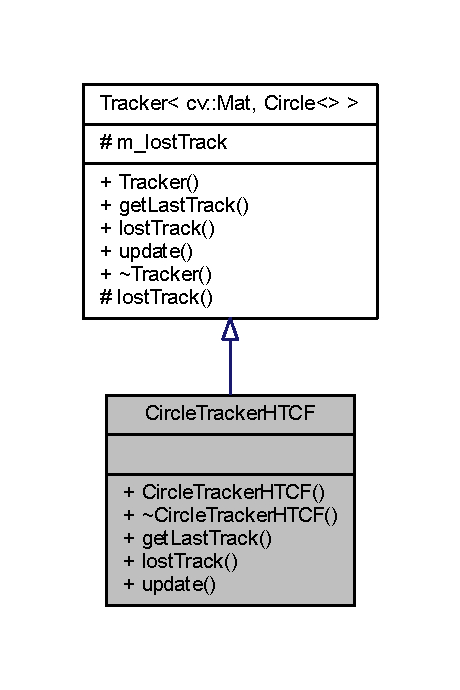
\includegraphics[width=221pt]{class_viscv_1_1_circle_tracker_h_t_c_f__inherit__graph}
\end{center}
\end{figure}


Collaboration diagram for Circle\+Tracker\+H\+T\+C\+F\+:
\nopagebreak
\begin{figure}[H]
\begin{center}
\leavevmode
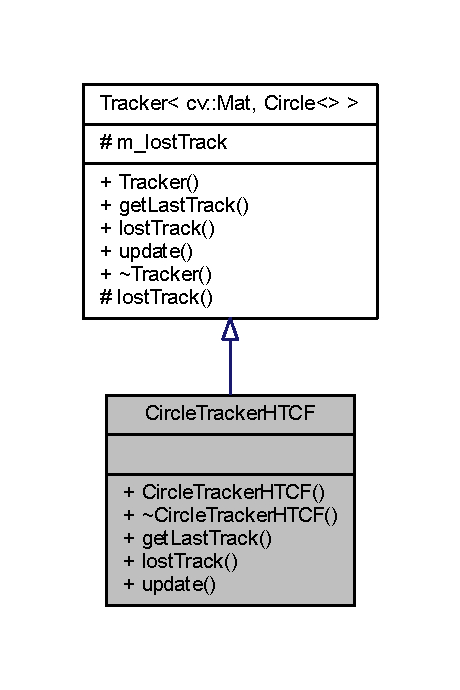
\includegraphics[width=221pt]{class_viscv_1_1_circle_tracker_h_t_c_f__coll__graph}
\end{center}
\end{figure}
\subsection*{Public Member Functions}
\begin{DoxyCompactItemize}
\item 
\hypertarget{class_viscv_1_1_circle_tracker_h_t_c_f_a925ba52aa4c7a0bbbedbcc3bc53b84ad}{}\hyperlink{class_viscv_1_1_circle_tracker_h_t_c_f_a925ba52aa4c7a0bbbedbcc3bc53b84ad}{Circle\+Tracker\+H\+T\+C\+F} (double x, double y, double radius)\label{class_viscv_1_1_circle_tracker_h_t_c_f_a925ba52aa4c7a0bbbedbcc3bc53b84ad}

\begin{DoxyCompactList}\small\item\em Constructor method. \end{DoxyCompactList}\item 
\hypertarget{class_viscv_1_1_circle_tracker_h_t_c_f_ab7bb92a06e7f731d7a4b1782f5b00d7b}{}virtual \hyperlink{class_viscv_1_1_circle_tracker_h_t_c_f_ab7bb92a06e7f731d7a4b1782f5b00d7b}{$\sim$\+Circle\+Tracker\+H\+T\+C\+F} ()\label{class_viscv_1_1_circle_tracker_h_t_c_f_ab7bb92a06e7f731d7a4b1782f5b00d7b}

\begin{DoxyCompactList}\small\item\em Destructor method. \end{DoxyCompactList}\item 
const \hyperlink{class_viscv_1_1_circle}{Circle} \& \hyperlink{class_viscv_1_1_circle_tracker_h_t_c_f_a0dcaebc9de9ff2ad85ef0a7ec554c363}{get\+Last\+Track} ()
\begin{DoxyCompactList}\small\item\em Returns a reference to the current estimated object state. \end{DoxyCompactList}\item 
bool \hyperlink{class_viscv_1_1_circle_tracker_h_t_c_f_ac7e0977fa702f98038bbe303df458a6c}{lost\+Track} () const 
\begin{DoxyCompactList}\small\item\em Returns true if the tracker lost the object track. \end{DoxyCompactList}\item 
\hypertarget{class_viscv_1_1_circle_tracker_h_t_c_f_ab233da15b6c7aad7d83c67057a558bd4}{}void \hyperlink{class_viscv_1_1_circle_tracker_h_t_c_f_ab233da15b6c7aad7d83c67057a558bd4}{update} (const \hyperlink{struct_vision_core_1_1_data_structures_1_1_frame}{Vision\+Core\+::\+Frame}$<$ cv\+::\+Mat $>$ \&frame)\label{class_viscv_1_1_circle_tracker_h_t_c_f_ab233da15b6c7aad7d83c67057a558bd4}

\begin{DoxyCompactList}\small\item\em Given an image (i.\+e. video frame), update the tracked objects. \end{DoxyCompactList}\end{DoxyCompactItemize}
\subsection*{Additional Inherited Members}


\subsection{Detailed Description}
Rastreador baseado na classe \hyperlink{class_viscv_1_1_circle_detector_h_t_c_f}{Circle\+Detector\+H\+T\+C\+F}. 

O rastreamento é feito limitando a região de interesse (R\+O\+I) de aplicação do detector em cada frame e filtrando o tamanho dos circulos. Ou seja, assume-\/se que houve apenas variação local da posição e tamanho do circulo

Definition at line 40 of file Circle\+Tracker\+H\+T\+C\+F.\+h.



\subsection{Member Function Documentation}
\hypertarget{class_viscv_1_1_circle_tracker_h_t_c_f_a0dcaebc9de9ff2ad85ef0a7ec554c363}{}\index{Viscv\+::\+Circle\+Tracker\+H\+T\+C\+F@{Viscv\+::\+Circle\+Tracker\+H\+T\+C\+F}!get\+Last\+Track@{get\+Last\+Track}}
\index{get\+Last\+Track@{get\+Last\+Track}!Viscv\+::\+Circle\+Tracker\+H\+T\+C\+F@{Viscv\+::\+Circle\+Tracker\+H\+T\+C\+F}}
\subsubsection[{get\+Last\+Track()}]{\setlength{\rightskip}{0pt plus 5cm}const {\bf Circle} \& get\+Last\+Track (
\begin{DoxyParamCaption}
{}
\end{DoxyParamCaption}
)\hspace{0.3cm}{\ttfamily [virtual]}}\label{class_viscv_1_1_circle_tracker_h_t_c_f_a0dcaebc9de9ff2ad85ef0a7ec554c363}


Returns a reference to the current estimated object state. 

This function is often call after calling the \hyperlink{class_viscv_1_1_circle_tracker_h_t_c_f_ab233da15b6c7aad7d83c67057a558bd4}{update()} method. The returned reference is usualy to a class member. 

Implements \hyperlink{class_vision_core_1_1_interfaces_1_1_tracker_a93ee7011307419e8c88db9f22d900657}{Tracker$<$ cv\+::\+Mat, Circle$<$$>$ $>$}.



Definition at line 54 of file Circle\+Tracker\+H\+T\+C\+F.\+cpp.

\hypertarget{class_viscv_1_1_circle_tracker_h_t_c_f_ac7e0977fa702f98038bbe303df458a6c}{}\index{Viscv\+::\+Circle\+Tracker\+H\+T\+C\+F@{Viscv\+::\+Circle\+Tracker\+H\+T\+C\+F}!lost\+Track@{lost\+Track}}
\index{lost\+Track@{lost\+Track}!Viscv\+::\+Circle\+Tracker\+H\+T\+C\+F@{Viscv\+::\+Circle\+Tracker\+H\+T\+C\+F}}
\subsubsection[{lost\+Track() const }]{\setlength{\rightskip}{0pt plus 5cm}bool lost\+Track (
\begin{DoxyParamCaption}
{}
\end{DoxyParamCaption}
) const\hspace{0.3cm}{\ttfamily [inline]}, {\ttfamily [virtual]}}\label{class_viscv_1_1_circle_tracker_h_t_c_f_ac7e0977fa702f98038bbe303df458a6c}


Returns true if the tracker lost the object track. 

The cause for loosing the object track is not specified by the interface. It can be caused by the object going out of image limits, becoming ocluded, or even due to a tracker error. 

Reimplemented from \hyperlink{class_vision_core_1_1_interfaces_1_1_tracker_af6217aec35983dca6dc39c91d08c1020}{Tracker$<$ cv\+::\+Mat, Circle$<$$>$ $>$}.



Definition at line 61 of file Circle\+Tracker\+H\+T\+C\+F.\+h.



The documentation for this class was generated from the following files\+:\begin{DoxyCompactItemize}
\item 
D\+:/\+F\+U\+R\+G/\+Software/\+Cv\+Works\+Release1/\+Components/\+Vision\+Implementation\+Cv/Circle\+Tracker\+H\+T\+C\+F.\+h\item 
D\+:/\+F\+U\+R\+G/\+Software/\+Cv\+Works\+Release1/\+Components/\+Vision\+Implementation\+Cv/Circle\+Tracker\+H\+T\+C\+F.\+cpp\end{DoxyCompactItemize}

\hypertarget{class_viscv_1_1_color_blob_detector_h_f}{}\section{Color\+Blob\+Detector\+H\+F Class Reference}
\label{class_viscv_1_1_color_blob_detector_h_f}\index{Color\+Blob\+Detector\+H\+F@{Color\+Blob\+Detector\+H\+F}}


Implementa um detector de blobs baseado em cor.  




{\ttfamily \#include $<$Color\+Blob\+Detector\+H\+F.\+h$>$}



Inheritance diagram for Color\+Blob\+Detector\+H\+F\+:
\nopagebreak
\begin{figure}[H]
\begin{center}
\leavevmode
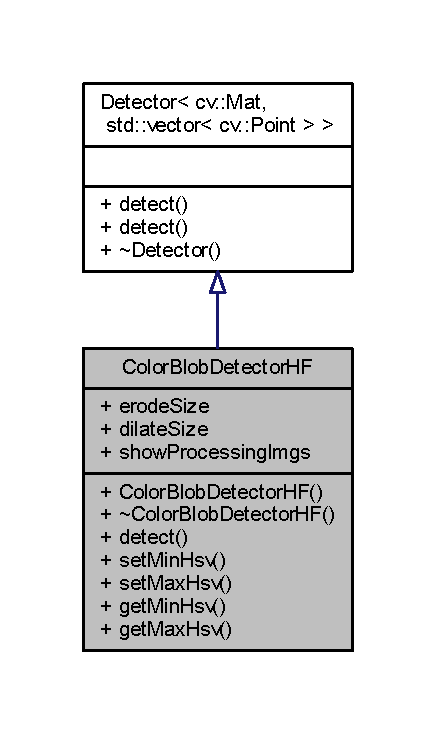
\includegraphics[width=209pt]{class_viscv_1_1_color_blob_detector_h_f__inherit__graph}
\end{center}
\end{figure}


Collaboration diagram for Color\+Blob\+Detector\+H\+F\+:
\nopagebreak
\begin{figure}[H]
\begin{center}
\leavevmode
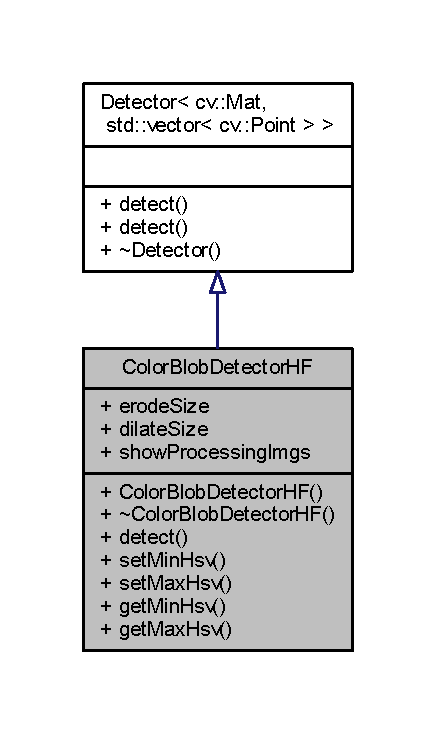
\includegraphics[width=209pt]{class_viscv_1_1_color_blob_detector_h_f__coll__graph}
\end{center}
\end{figure}
\subsection*{Public Member Functions}
\begin{DoxyCompactItemize}
\item 
\hypertarget{class_viscv_1_1_color_blob_detector_h_f_a22080136627bd90459c3a7cc68db48fc}{}\hyperlink{class_viscv_1_1_color_blob_detector_h_f_a22080136627bd90459c3a7cc68db48fc}{Color\+Blob\+Detector\+H\+F} (void)\label{class_viscv_1_1_color_blob_detector_h_f_a22080136627bd90459c3a7cc68db48fc}

\begin{DoxyCompactList}\small\item\em Construtor default. \end{DoxyCompactList}\item 
\hypertarget{class_viscv_1_1_color_blob_detector_h_f_a1a287459fc13984350ba9e1d68eac14e}{}virtual \hyperlink{class_viscv_1_1_color_blob_detector_h_f_a1a287459fc13984350ba9e1d68eac14e}{$\sim$\+Color\+Blob\+Detector\+H\+F} (void)\label{class_viscv_1_1_color_blob_detector_h_f_a1a287459fc13984350ba9e1d68eac14e}

\begin{DoxyCompactList}\small\item\em Destrutor. \end{DoxyCompactList}\item 
\hypertarget{class_viscv_1_1_color_blob_detector_h_f_a76311b08b5cb9df65524e070e9c15048}{}std\+::vector$<$ std\+::vector$<$ cv\+::\+Point $>$ $>$ \hyperlink{class_viscv_1_1_color_blob_detector_h_f_a76311b08b5cb9df65524e070e9c15048}{detect} (const cv\+::\+Mat \&img) const \label{class_viscv_1_1_color_blob_detector_h_f_a76311b08b5cb9df65524e070e9c15048}

\begin{DoxyCompactList}\small\item\em Detecta blobs em uma imagem. \end{DoxyCompactList}\item 
\hypertarget{class_viscv_1_1_color_blob_detector_h_f_ae985929bdd9605ac5ab2460f6b824a97}{}void \hyperlink{class_viscv_1_1_color_blob_detector_h_f_ae985929bdd9605ac5ab2460f6b824a97}{set\+Min\+Hsv} (const cv\+::\+Scalar \&min\+Hsv\+\_\+)\label{class_viscv_1_1_color_blob_detector_h_f_ae985929bdd9605ac5ab2460f6b824a97}

\begin{DoxyCompactList}\small\item\em Define a cor mínima que será filtrada. \end{DoxyCompactList}\item 
\hypertarget{class_viscv_1_1_color_blob_detector_h_f_a842c89f58a06bc5d08b555e0ebcce3a4}{}void \hyperlink{class_viscv_1_1_color_blob_detector_h_f_a842c89f58a06bc5d08b555e0ebcce3a4}{set\+Max\+Hsv} (const cv\+::\+Scalar \&max\+Hsv\+\_\+)\label{class_viscv_1_1_color_blob_detector_h_f_a842c89f58a06bc5d08b555e0ebcce3a4}

\begin{DoxyCompactList}\small\item\em Define a cor máxima que será filtrada. \end{DoxyCompactList}\item 
\hypertarget{class_viscv_1_1_color_blob_detector_h_f_a34a1242cfaf748ff5c2ebd03b2e9daf6}{}const cv\+::\+Scalar \& \hyperlink{class_viscv_1_1_color_blob_detector_h_f_a34a1242cfaf748ff5c2ebd03b2e9daf6}{get\+Min\+Hsv} () const \label{class_viscv_1_1_color_blob_detector_h_f_a34a1242cfaf748ff5c2ebd03b2e9daf6}

\begin{DoxyCompactList}\small\item\em Retorna a cor mínima que será filtrada. \end{DoxyCompactList}\item 
\hypertarget{class_viscv_1_1_color_blob_detector_h_f_a762033ea84177602ff2b152b5d144c1b}{}const cv\+::\+Scalar \& \hyperlink{class_viscv_1_1_color_blob_detector_h_f_a762033ea84177602ff2b152b5d144c1b}{get\+Max\+Hsv} () const \label{class_viscv_1_1_color_blob_detector_h_f_a762033ea84177602ff2b152b5d144c1b}

\begin{DoxyCompactList}\small\item\em Retorna a cor máxima que será filtrada. \end{DoxyCompactList}\end{DoxyCompactItemize}
\subsection*{Public Attributes}
\begin{DoxyCompactItemize}
\item 
\hypertarget{class_viscv_1_1_color_blob_detector_h_f_ade892534cd32ce4ae635c5d79c76dbbf}{}int \hyperlink{class_viscv_1_1_color_blob_detector_h_f_ade892534cd32ce4ae635c5d79c76dbbf}{erode\+Size}\label{class_viscv_1_1_color_blob_detector_h_f_ade892534cd32ce4ae635c5d79c76dbbf}

\begin{DoxyCompactList}\small\item\em Diâmetro do kernel (circular) usado na erosão. \end{DoxyCompactList}\item 
\hypertarget{class_viscv_1_1_color_blob_detector_h_f_ad0b5e1ba575b162ef99943983c9ca931}{}int \hyperlink{class_viscv_1_1_color_blob_detector_h_f_ad0b5e1ba575b162ef99943983c9ca931}{dilate\+Size}\label{class_viscv_1_1_color_blob_detector_h_f_ad0b5e1ba575b162ef99943983c9ca931}

\begin{DoxyCompactList}\small\item\em Diâmetro do kernel (circular) usado na dilatação. \end{DoxyCompactList}\item 
\hypertarget{class_viscv_1_1_color_blob_detector_h_f_ad56f3dc42f92c3f920caed1aec8ead03}{}bool \hyperlink{class_viscv_1_1_color_blob_detector_h_f_ad56f3dc42f92c3f920caed1aec8ead03}{show\+Processing\+Imgs}\label{class_viscv_1_1_color_blob_detector_h_f_ad56f3dc42f92c3f920caed1aec8ead03}

\begin{DoxyCompactList}\small\item\em Define se as imagens intermediárias de processamento devem ser mostradas. \end{DoxyCompactList}\end{DoxyCompactItemize}
\subsection*{Additional Inherited Members}


\subsection{Detailed Description}
Implementa um detector de blobs baseado em cor. 

O detector executa os seguintes passos\+: 1) Aplica um filtro de cor, baseado em um mínimo e máximo. 2) Aplica dilatação e erosão para fechar buracos e eliminar pequenos blobs. 3) Encontra blobs 4) Filtra blobs baseado em características (tamanho e forma)

Obs\+: A Open\+Cv possui uma implementação de detector de blobs na classe cv\+::\+Simple\+Blob\+Detector. \begin{Desc}
\item[Examples\+: ]\par
\hyperlink{_vision_tests_2main_8cpp-example}{Vision\+Tests/main.\+cpp}.\end{Desc}


Definition at line 45 of file Color\+Blob\+Detector\+H\+F.\+h.



The documentation for this class was generated from the following files\+:\begin{DoxyCompactItemize}
\item 
D\+:/\+F\+U\+R\+G/\+Software/\+Cv\+Works\+Release1/\+Components/\+Vision\+Implementation\+Cv/Color\+Blob\+Detector\+H\+F.\+h\item 
D\+:/\+F\+U\+R\+G/\+Software/\+Cv\+Works\+Release1/\+Components/\+Vision\+Implementation\+Cv/Color\+Blob\+Detector\+H\+F.\+cpp\end{DoxyCompactItemize}

\hypertarget{class_viscv_1_1_cv_image_g_u_i}{}\section{Cv\+Image\+G\+U\+I Class Reference}
\label{class_viscv_1_1_cv_image_g_u_i}\index{Cv\+Image\+G\+U\+I@{Cv\+Image\+G\+U\+I}}


Esta classe cria uma janela para exibição de imagens.  




{\ttfamily \#include $<$Cv\+Image\+G\+U\+I.\+h$>$}



Collaboration diagram for Cv\+Image\+G\+U\+I\+:
\nopagebreak
\begin{figure}[H]
\begin{center}
\leavevmode
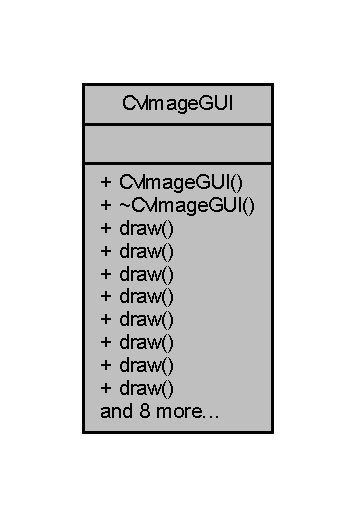
\includegraphics[width=171pt]{class_viscv_1_1_cv_image_g_u_i__coll__graph}
\end{center}
\end{figure}
\subsection*{Public Member Functions}
\begin{DoxyCompactItemize}
\item 
\hypertarget{class_viscv_1_1_cv_image_g_u_i_a906aae50fd4edb5555d10f7d0ae4f906}{}\hyperlink{class_viscv_1_1_cv_image_g_u_i_a906aae50fd4edb5555d10f7d0ae4f906}{Cv\+Image\+G\+U\+I} (cv\+::\+Mat img=cv\+::\+Mat())\label{class_viscv_1_1_cv_image_g_u_i_a906aae50fd4edb5555d10f7d0ae4f906}

\begin{DoxyCompactList}\small\item\em Constructor method. \end{DoxyCompactList}\item 
\hypertarget{class_viscv_1_1_cv_image_g_u_i_aede5851d62dbd49ce5e4974833c387e0}{}virtual \hyperlink{class_viscv_1_1_cv_image_g_u_i_aede5851d62dbd49ce5e4974833c387e0}{$\sim$\+Cv\+Image\+G\+U\+I} ()\label{class_viscv_1_1_cv_image_g_u_i_aede5851d62dbd49ce5e4974833c387e0}

\begin{DoxyCompactList}\small\item\em Destructor method. \end{DoxyCompactList}\item 
\hypertarget{class_viscv_1_1_cv_image_g_u_i_a275ce8772494b98eaf1f08bacd055870}{}void {\bfseries draw} (const std\+::vector$<$ cv\+::\+Rect $>$ \&rectangles)\label{class_viscv_1_1_cv_image_g_u_i_a275ce8772494b98eaf1f08bacd055870}

\item 
\hypertarget{class_viscv_1_1_cv_image_g_u_i_a1fbcf47e959e0c4b227793f4c9e54670}{}void {\bfseries draw} (const std\+::vector$<$ cv\+::\+Point2f $>$ \&points)\label{class_viscv_1_1_cv_image_g_u_i_a1fbcf47e959e0c4b227793f4c9e54670}

\item 
\hypertarget{class_viscv_1_1_cv_image_g_u_i_aee8552ffd73cced2736d5accbc6687a0}{}void {\bfseries draw} (const cv\+::\+Rect \&rectangle)\label{class_viscv_1_1_cv_image_g_u_i_aee8552ffd73cced2736d5accbc6687a0}

\item 
\hypertarget{class_viscv_1_1_cv_image_g_u_i_af02e64519961d07a84cb810f36d61a88}{}void {\bfseries draw} (const std\+::list$<$ cv\+::\+Rect $>$ \&rectangles)\label{class_viscv_1_1_cv_image_g_u_i_af02e64519961d07a84cb810f36d61a88}

\item 
\hypertarget{class_viscv_1_1_cv_image_g_u_i_a4d8d0d54dc0719bbf9246d098ec4f593}{}void {\bfseries draw} (const cv\+::\+Point2f \&point)\label{class_viscv_1_1_cv_image_g_u_i_a4d8d0d54dc0719bbf9246d098ec4f593}

\item 
\hypertarget{class_viscv_1_1_cv_image_g_u_i_ab3ee7a0c951aaa36d3f5e05b43d3a23d}{}void {\bfseries draw} (const \hyperlink{class_viscv_1_1_circle}{Circle}$<$$>$ \&c)\label{class_viscv_1_1_cv_image_g_u_i_ab3ee7a0c951aaa36d3f5e05b43d3a23d}

\item 
\hypertarget{class_viscv_1_1_cv_image_g_u_i_abc977e1456da5351fc8bc2ca0ed4c1e8}{}void {\bfseries draw} (const std\+::vector$<$ \hyperlink{class_viscv_1_1_circle}{Circle}$<$$>$$>$ \&circles)\label{class_viscv_1_1_cv_image_g_u_i_abc977e1456da5351fc8bc2ca0ed4c1e8}

\item 
\hypertarget{class_viscv_1_1_cv_image_g_u_i_a11d55a5b1a3838451b744db3aebac34d}{}void {\bfseries draw} (const std\+::vector$<$ std\+::vector$<$ cv\+::\+Point $>$$>$ \&contours)\label{class_viscv_1_1_cv_image_g_u_i_a11d55a5b1a3838451b744db3aebac34d}

\item 
\hypertarget{class_viscv_1_1_cv_image_g_u_i_af57efcd8e43090aee7e10a77c9797c20}{}void {\bfseries draw} (const \hyperlink{class_viscv_1_1_a_r_tag}{A\+R\+Tag} \&tag)\label{class_viscv_1_1_cv_image_g_u_i_af57efcd8e43090aee7e10a77c9797c20}

\item 
\hypertarget{class_viscv_1_1_cv_image_g_u_i_a188abfb4bdc75af2a09d9d1cc9abb92d}{}void {\bfseries draw} (const std\+::vector$<$ \hyperlink{class_viscv_1_1_a_r_tag}{A\+R\+Tag} $>$ \&tags)\label{class_viscv_1_1_cv_image_g_u_i_a188abfb4bdc75af2a09d9d1cc9abb92d}

\item 
\hypertarget{class_viscv_1_1_cv_image_g_u_i_a819ad5554e3d1e8d908c4511aff60d36}{}void {\bfseries draw} (const std\+::map$<$ long, cv\+::\+Rect $>$ \&objects)\label{class_viscv_1_1_cv_image_g_u_i_a819ad5554e3d1e8d908c4511aff60d36}

\item 
\hypertarget{class_viscv_1_1_cv_image_g_u_i_a2032a58da0bc543d0fc6945973108674}{}void \hyperlink{class_viscv_1_1_cv_image_g_u_i_a2032a58da0bc543d0fc6945973108674}{draw} (const std\+::string \&text, const double col\+Position=0.\+5, const double row\+Position=0.\+5, double size=1)\label{class_viscv_1_1_cv_image_g_u_i_a2032a58da0bc543d0fc6945973108674}

\begin{DoxyCompactList}\small\item\em Escreve um texto na imagem. \end{DoxyCompactList}\item 
\hypertarget{class_viscv_1_1_cv_image_g_u_i_a4b148f40a95444d5669406b918ad2f52}{}void {\bfseries show} ()\label{class_viscv_1_1_cv_image_g_u_i_a4b148f40a95444d5669406b918ad2f52}

\item 
\hypertarget{class_viscv_1_1_cv_image_g_u_i_a128346d089624c27ffddb80f0526dc24}{}const cv\+::\+Mat \& \hyperlink{class_viscv_1_1_cv_image_g_u_i_a128346d089624c27ffddb80f0526dc24}{get\+Img} () const \label{class_viscv_1_1_cv_image_g_u_i_a128346d089624c27ffddb80f0526dc24}

\begin{DoxyCompactList}\small\item\em Returns the value of member \textquotesingle{}m\+\_\+img\textquotesingle{}. \end{DoxyCompactList}\item 
\hypertarget{class_viscv_1_1_cv_image_g_u_i_a4ae2d7fd59643d69dfe83dff37582501}{}void \hyperlink{class_viscv_1_1_cv_image_g_u_i_a4ae2d7fd59643d69dfe83dff37582501}{set\+Img} (const cv\+::\+Mat \&img)\label{class_viscv_1_1_cv_image_g_u_i_a4ae2d7fd59643d69dfe83dff37582501}

\begin{DoxyCompactList}\small\item\em Set the value of member \textquotesingle{}m\+\_\+img\textquotesingle{} to \textquotesingle{}img\textquotesingle{}. \end{DoxyCompactList}\item 
\hypertarget{class_viscv_1_1_cv_image_g_u_i_afb48ea0df1b0f3d228839536031af917}{}const std\+::string \hyperlink{class_viscv_1_1_cv_image_g_u_i_afb48ea0df1b0f3d228839536031af917}{get\+Window\+Name} () const \label{class_viscv_1_1_cv_image_g_u_i_afb48ea0df1b0f3d228839536031af917}

\begin{DoxyCompactList}\small\item\em Returns the value of member \textquotesingle{}m\+\_\+window\+Name\textquotesingle{}. \end{DoxyCompactList}\end{DoxyCompactItemize}


\subsection{Detailed Description}
Esta classe cria uma janela para exibição de imagens. 

Possui métodos que facilitam a sobreposição de outros objetos (pontos, linhas, retangulos, etc) na imagem. \begin{Desc}
\item[Examples\+: ]\par
\hyperlink{_vision_tests_2main_8cpp-example}{Vision\+Tests/main.\+cpp}.\end{Desc}


Definition at line 40 of file Cv\+Image\+G\+U\+I.\+h.



The documentation for this class was generated from the following files\+:\begin{DoxyCompactItemize}
\item 
D\+:/\+F\+U\+R\+G/\+Software/\+Cv\+Works\+Release1/\+Components/\+Vision\+Implementation\+Cv/Cv\+Image\+G\+U\+I.\+h\item 
D\+:/\+F\+U\+R\+G/\+Software/\+Cv\+Works\+Release1/\+Components/\+Vision\+Implementation\+Cv/Cv\+Image\+G\+U\+I.\+cpp\end{DoxyCompactItemize}

\hypertarget{class_viscv_1_1_dataset_f_d_d_b}{}\section{Dataset\+F\+D\+D\+B Class Reference}
\label{class_viscv_1_1_dataset_f_d_d_b}\index{Dataset\+F\+D\+D\+B@{Dataset\+F\+D\+D\+B}}


Dataset público de várias imagens contendo pessoas em ambientes do dia-\/a-\/dia.  




{\ttfamily \#include $<$Dataset\+F\+D\+D\+B.\+h$>$}



Inheritance diagram for Dataset\+F\+D\+D\+B\+:
\nopagebreak
\begin{figure}[H]
\begin{center}
\leavevmode
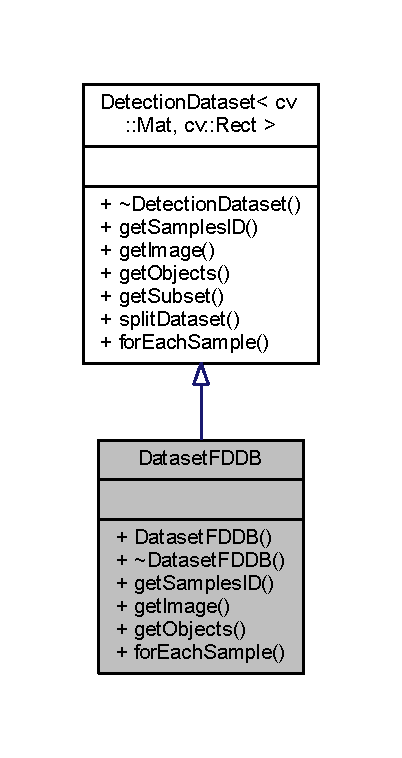
\includegraphics[width=193pt]{class_viscv_1_1_dataset_f_d_d_b__inherit__graph}
\end{center}
\end{figure}


Collaboration diagram for Dataset\+F\+D\+D\+B\+:
\nopagebreak
\begin{figure}[H]
\begin{center}
\leavevmode
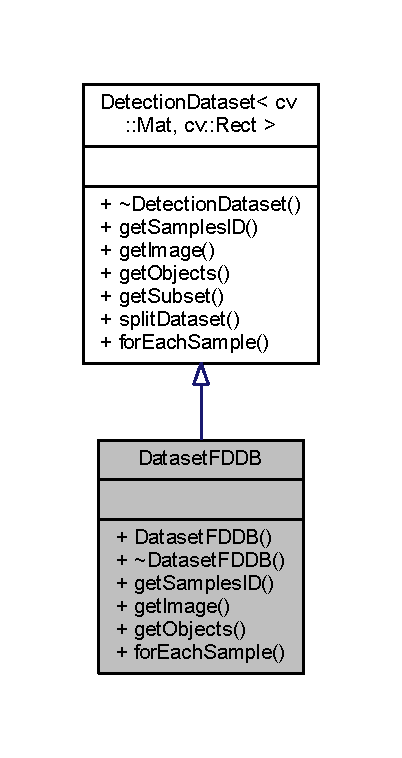
\includegraphics[width=193pt]{class_viscv_1_1_dataset_f_d_d_b__coll__graph}
\end{center}
\end{figure}
\subsection*{Public Member Functions}
\begin{DoxyCompactItemize}
\item 
\hyperlink{class_viscv_1_1_dataset_f_d_d_b_a1f73293d1c0506448791946f30d710ff}{Dataset\+F\+D\+D\+B} (const std\+::string base\+Dir, const std\+::string fold)
\begin{DoxyCompactList}\small\item\em Construtor. \end{DoxyCompactList}\item 
\hypertarget{class_viscv_1_1_dataset_f_d_d_b_af7f8d85c565cd9e7aa5a8b2f5985c134}{}virtual \hyperlink{class_viscv_1_1_dataset_f_d_d_b_af7f8d85c565cd9e7aa5a8b2f5985c134}{$\sim$\+Dataset\+F\+D\+D\+B} (void)\label{class_viscv_1_1_dataset_f_d_d_b_af7f8d85c565cd9e7aa5a8b2f5985c134}

\begin{DoxyCompactList}\small\item\em Destrutor. \end{DoxyCompactList}\item 
\hypertarget{class_viscv_1_1_dataset_f_d_d_b_a8f2602813f5b8c2c6512690efbabb2df}{}virtual std\+::vector$<$ std\+::string $>$ \hyperlink{class_viscv_1_1_dataset_f_d_d_b_a8f2602813f5b8c2c6512690efbabb2df}{get\+Samples\+I\+D} () const \label{class_viscv_1_1_dataset_f_d_d_b_a8f2602813f5b8c2c6512690efbabb2df}

\begin{DoxyCompactList}\small\item\em Retorna um vetor com os identificadores de todas as amostras contidas no dataset. \end{DoxyCompactList}\item 
\hypertarget{class_viscv_1_1_dataset_f_d_d_b_a64f0340b5a377d18c5199f61a8ee7ffd}{}virtual std\+::shared\+\_\+ptr$<$ cv\+::\+Mat $>$ \hyperlink{class_viscv_1_1_dataset_f_d_d_b_a64f0340b5a377d18c5199f61a8ee7ffd}{get\+Image} (const std\+::string \&sample\+I\+D) const \label{class_viscv_1_1_dataset_f_d_d_b_a64f0340b5a377d18c5199f61a8ee7ffd}

\begin{DoxyCompactList}\small\item\em Retorna um ponteiro para a imagem de uma amostra. \end{DoxyCompactList}\item 
\hypertarget{class_viscv_1_1_dataset_f_d_d_b_a8c1fe796c01ff8d85626dd85e6a45418}{}virtual std\+::vector$<$ cv\+::\+Rect $>$ \hyperlink{class_viscv_1_1_dataset_f_d_d_b_a8c1fe796c01ff8d85626dd85e6a45418}{get\+Objects} (const std\+::string \&sample\+I\+D) const \label{class_viscv_1_1_dataset_f_d_d_b_a8c1fe796c01ff8d85626dd85e6a45418}

\begin{DoxyCompactList}\small\item\em Retorna uma lista com os objetos contidos na imagem de uma amostra. \end{DoxyCompactList}\item 
virtual void \hyperlink{class_viscv_1_1_dataset_f_d_d_b_a91e8a6b561989bd8507dbb120957786d}{for\+Each\+Sample} (std\+::function$<$ void(cv\+::\+Mat \&, std\+::vector$<$ cv\+::\+Rect $>$ \&, const std\+::string \&)$>$ funct)
\begin{DoxyCompactList}\small\item\em Executa uma função para cada amostra do dataset. \end{DoxyCompactList}\end{DoxyCompactItemize}
\subsection*{Additional Inherited Members}


\subsection{Detailed Description}
Dataset público de várias imagens contendo pessoas em ambientes do dia-\/a-\/dia. 

Utilizado principalmente para detecção de faces. Para cada imagem contida no dataset existe uma anotação (extraidas de um arquivo texto) que indica a localização das faces. \begin{Desc}
\item[Examples\+: ]\par
\hyperlink{_vision_tests_2main_8cpp-example}{Vision\+Tests/main.\+cpp}.\end{Desc}


Definition at line 40 of file Dataset\+F\+D\+D\+B.\+h.



\subsection{Constructor \& Destructor Documentation}
\hypertarget{class_viscv_1_1_dataset_f_d_d_b_a1f73293d1c0506448791946f30d710ff}{}\index{Viscv\+::\+Dataset\+F\+D\+D\+B@{Viscv\+::\+Dataset\+F\+D\+D\+B}!Dataset\+F\+D\+D\+B@{Dataset\+F\+D\+D\+B}}
\index{Dataset\+F\+D\+D\+B@{Dataset\+F\+D\+D\+B}!Viscv\+::\+Dataset\+F\+D\+D\+B@{Viscv\+::\+Dataset\+F\+D\+D\+B}}
\subsubsection[{Dataset\+F\+D\+D\+B(const std\+::string base\+Dir, const std\+::string fold)}]{\setlength{\rightskip}{0pt plus 5cm}{\bf Dataset\+F\+D\+D\+B} (
\begin{DoxyParamCaption}
\item[{const std\+::string}]{base\+Dir, }
\item[{const std\+::string}]{fold}
\end{DoxyParamCaption}
)}\label{class_viscv_1_1_dataset_f_d_d_b_a1f73293d1c0506448791946f30d710ff}


Construtor. 

É necessário informar o diretório onde está o dataset e o path completo do arquivo texto conténdo a lista das imagens e anotações de cada imagem (fornecido junto com o dataset). Exemplo\+: \hyperlink{class_viscv_1_1_dataset_f_d_d_b}{Dataset\+F\+D\+D\+B} db(\char`\"{}\+E\+:/\+F\+U\+R\+G/\+Datasets/\+F\+D\+D\+B/\char`\"{},\char`\"{}\+E\+:/\+F\+U\+R\+G/\+Datasets/\+F\+D\+D\+B-\/folds/\+F\+D\+D\+B-\/fold-\/01-\/ellipse\+List.\+txt\char`\"{}); 

Definition at line 33 of file Dataset\+F\+D\+D\+B.\+cpp.



\subsection{Member Function Documentation}
\hypertarget{class_viscv_1_1_dataset_f_d_d_b_a91e8a6b561989bd8507dbb120957786d}{}\index{Viscv\+::\+Dataset\+F\+D\+D\+B@{Viscv\+::\+Dataset\+F\+D\+D\+B}!for\+Each\+Sample@{for\+Each\+Sample}}
\index{for\+Each\+Sample@{for\+Each\+Sample}!Viscv\+::\+Dataset\+F\+D\+D\+B@{Viscv\+::\+Dataset\+F\+D\+D\+B}}
\subsubsection[{for\+Each\+Sample(std\+::function$<$ void(cv\+::\+Mat \&, std\+::vector$<$ cv\+::\+Rect $>$ \&, const std\+::string \&)$>$ funct)}]{\setlength{\rightskip}{0pt plus 5cm}void for\+Each\+Sample (
\begin{DoxyParamCaption}
\item[{std\+::function$<$ void(cv\+::\+Mat \&, std\+::vector$<$ cv\+::\+Rect $>$ \&, const std\+::string \&)$>$}]{funct}
\end{DoxyParamCaption}
)\hspace{0.3cm}{\ttfamily [virtual]}}\label{class_viscv_1_1_dataset_f_d_d_b_a91e8a6b561989bd8507dbb120957786d}


Executa uma função para cada amostra do dataset. 

Esta função abre cada uma das imagens do dataset, extrai as informações de anotações (locais das faces), e chama a função passada como argumento. O sample\+Id de cada amostra é o nome do arquivo da imagem. 

Definition at line 70 of file Dataset\+F\+D\+D\+B.\+cpp.



The documentation for this class was generated from the following files\+:\begin{DoxyCompactItemize}
\item 
D\+:/\+F\+U\+R\+G/\+Software/\+Cv\+Works\+Release1/\+Components/\+Vision\+Implementation\+Cv/Dataset\+F\+D\+D\+B.\+h\item 
D\+:/\+F\+U\+R\+G/\+Software/\+Cv\+Works\+Release1/\+Components/\+Vision\+Implementation\+Cv/Dataset\+F\+D\+D\+B.\+cpp\end{DoxyCompactItemize}

\hypertarget{class_dataset_fire}{}\section{Dataset\+Fire Class Reference}
\label{class_dataset_fire}\index{Dataset\+Fire@{Dataset\+Fire}}


{\ttfamily \#include $<$Dataset\+Fire.\+h$>$}



Inheritance diagram for Dataset\+Fire\+:
\nopagebreak
\begin{figure}[H]
\begin{center}
\leavevmode
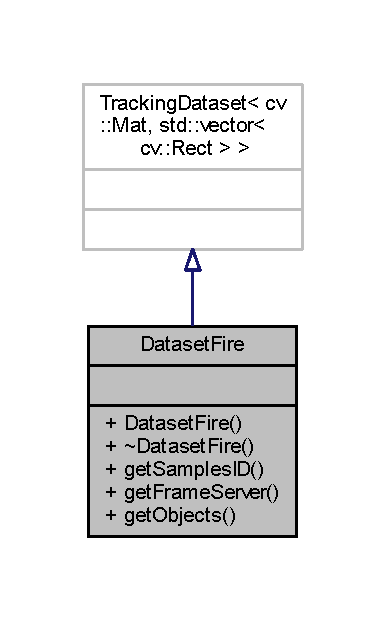
\includegraphics[width=185pt]{class_dataset_fire__inherit__graph}
\end{center}
\end{figure}


Collaboration diagram for Dataset\+Fire\+:
\nopagebreak
\begin{figure}[H]
\begin{center}
\leavevmode
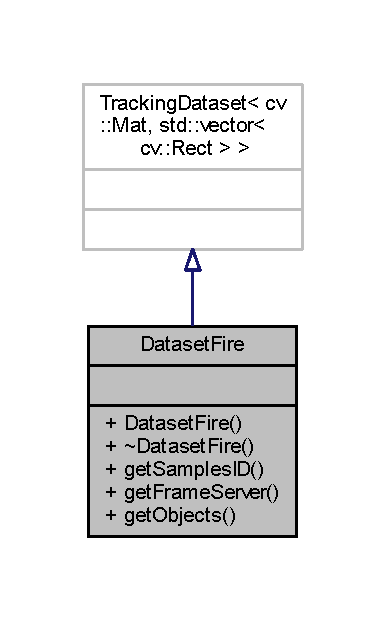
\includegraphics[width=185pt]{class_dataset_fire__coll__graph}
\end{center}
\end{figure}
\subsection*{Public Member Functions}
\begin{DoxyCompactItemize}
\item 
\hyperlink{class_dataset_fire_aca72c752d0b957c6fd33bc4cc83aa48c}{Dataset\+Fire} (const std\+::string base\+Dir)
\begin{DoxyCompactList}\small\item\em Construtor. \end{DoxyCompactList}\item 
\hypertarget{class_dataset_fire_ae8c160d80a95ff180eb7a5e9c6f7e1a9}{}virtual \hyperlink{class_dataset_fire_ae8c160d80a95ff180eb7a5e9c6f7e1a9}{$\sim$\+Dataset\+Fire} (void)\label{class_dataset_fire_ae8c160d80a95ff180eb7a5e9c6f7e1a9}

\begin{DoxyCompactList}\small\item\em Destrutor. \end{DoxyCompactList}\item 
\hypertarget{class_dataset_fire_a8f2602813f5b8c2c6512690efbabb2df}{}virtual std\+::vector$<$ std\+::string $>$ \hyperlink{class_dataset_fire_a8f2602813f5b8c2c6512690efbabb2df}{get\+Samples\+I\+D} () const \label{class_dataset_fire_a8f2602813f5b8c2c6512690efbabb2df}

\begin{DoxyCompactList}\small\item\em Retorna um vetor com os identificadores de todas as amostras contidas no dataset. \end{DoxyCompactList}\item 
virtual \hyperlink{class_vision_core_1_1_interfaces_1_1_frame_server}{Frame\+Server}$<$ cv\+::\+Mat $>$ $\ast$ \hyperlink{class_dataset_fire_a367c3fb2404cb97f5234542de8379d6d}{get\+Frame\+Server} (const std\+::string \&sample\+I\+D) const 
\begin{DoxyCompactList}\small\item\em Retorna um ponteiro para a imagem de uma amostra. \end{DoxyCompactList}\item 
virtual std\+::vector$<$ std\+::vector$<$ cv\+::\+Rect $>$ $>$ \hyperlink{class_dataset_fire_a5bd8609aff7b688bccfc3ed6e8299159}{get\+Objects} (const std\+::string \&sample\+I\+D) const 
\begin{DoxyCompactList}\small\item\em Retorna uma lista com os objetos contidos na imagem de uma amostra. \end{DoxyCompactList}\end{DoxyCompactItemize}


\subsection{Detailed Description}
The fire dataset is a set of annotated videos. The annotations are in a rectangle shape. One frame can contain 0 or more annotated regions. \begin{Desc}
\item[Examples\+: ]\par
\hyperlink{_vision_tests_2main_8cpp-example}{Vision\+Tests/main.\+cpp}.\end{Desc}


Definition at line 43 of file Dataset\+Fire.\+h.



\subsection{Constructor \& Destructor Documentation}
\hypertarget{class_dataset_fire_aca72c752d0b957c6fd33bc4cc83aa48c}{}\index{Dataset\+Fire@{Dataset\+Fire}!Dataset\+Fire@{Dataset\+Fire}}
\index{Dataset\+Fire@{Dataset\+Fire}!Dataset\+Fire@{Dataset\+Fire}}
\subsubsection[{Dataset\+Fire(const std\+::string base\+Dir)}]{\setlength{\rightskip}{0pt plus 5cm}{\bf Dataset\+Fire} (
\begin{DoxyParamCaption}
\item[{const std\+::string}]{base\+Dir}
\end{DoxyParamCaption}
)}\label{class_dataset_fire_aca72c752d0b957c6fd33bc4cc83aa48c}


Construtor. 

É necessário informar o diretório onde está o dataset e o path completo do arquivo texto conténdo a lista das imagens e anotações de cada imagem (fornecido junto com o dataset). Exemplo\+: 

Definition at line 36 of file Dataset\+Fire.\+cpp.



\subsection{Member Function Documentation}
\hypertarget{class_dataset_fire_a367c3fb2404cb97f5234542de8379d6d}{}\index{Dataset\+Fire@{Dataset\+Fire}!get\+Frame\+Server@{get\+Frame\+Server}}
\index{get\+Frame\+Server@{get\+Frame\+Server}!Dataset\+Fire@{Dataset\+Fire}}
\subsubsection[{get\+Frame\+Server(const std\+::string \&sample\+I\+D) const }]{\setlength{\rightskip}{0pt plus 5cm}{\bf Frame\+Server}$<$ cv\+::\+Mat $>$ $\ast$ get\+Frame\+Server (
\begin{DoxyParamCaption}
\item[{const std\+::string \&}]{sample\+I\+D}
\end{DoxyParamCaption}
) const\hspace{0.3cm}{\ttfamily [virtual]}}\label{class_dataset_fire_a367c3fb2404cb97f5234542de8379d6d}


Retorna um ponteiro para a imagem de uma amostra. 

Retorna um video. 

Definition at line 72 of file Dataset\+Fire.\+cpp.

\hypertarget{class_dataset_fire_a5bd8609aff7b688bccfc3ed6e8299159}{}\index{Dataset\+Fire@{Dataset\+Fire}!get\+Objects@{get\+Objects}}
\index{get\+Objects@{get\+Objects}!Dataset\+Fire@{Dataset\+Fire}}
\subsubsection[{get\+Objects(const std\+::string \&sample\+I\+D) const }]{\setlength{\rightskip}{0pt plus 5cm}std\+::vector$<$ std\+::vector$<$ cv\+::\+Rect $>$ $>$ get\+Objects (
\begin{DoxyParamCaption}
\item[{const std\+::string \&}]{sample\+I\+D}
\end{DoxyParamCaption}
) const\hspace{0.3cm}{\ttfamily [virtual]}}\label{class_dataset_fire_a5bd8609aff7b688bccfc3ed6e8299159}


Retorna uma lista com os objetos contidos na imagem de uma amostra. 

Retorna um vetor com os objetos contidos na imagem de uma amostra. 

Definition at line 79 of file Dataset\+Fire.\+cpp.



The documentation for this class was generated from the following files\+:\begin{DoxyCompactItemize}
\item 
D\+:/\+F\+U\+R\+G/\+Software/\+Cv\+Works\+Release1/\+Components/\+Fire\+Detector/Dataset\+Fire.\+h\item 
D\+:/\+F\+U\+R\+G/\+Software/\+Cv\+Works\+Release1/\+Components/\+Fire\+Detector/Dataset\+Fire.\+cpp\end{DoxyCompactItemize}

\hypertarget{struct_vision_core_1_1_abstractions_1_1_detection_data}{}\section{Detection\+Data$<$ T\+Obj $>$ Struct Template Reference}
\label{struct_vision_core_1_1_abstractions_1_1_detection_data}\index{Detection\+Data$<$ T\+Obj $>$@{Detection\+Data$<$ T\+Obj $>$}}


Simple structure that stores data related to a detection (used in Detection\+Logger).  




{\ttfamily \#include $<$Vision\+Abstractions.\+h$>$}



Collaboration diagram for Detection\+Data$<$ T\+Obj $>$\+:
\nopagebreak
\begin{figure}[H]
\begin{center}
\leavevmode
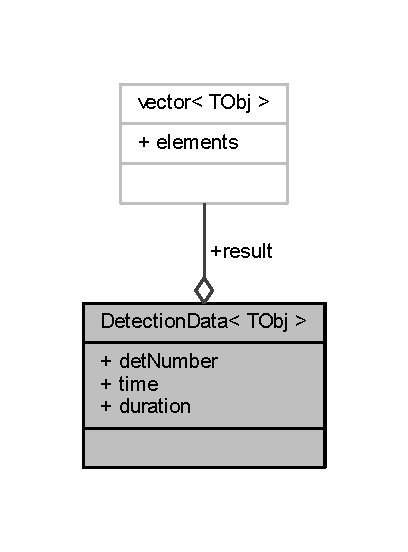
\includegraphics[width=196pt]{struct_vision_core_1_1_abstractions_1_1_detection_data__coll__graph}
\end{center}
\end{figure}
\subsection*{Public Attributes}
\begin{DoxyCompactItemize}
\item 
\hypertarget{struct_vision_core_1_1_abstractions_1_1_detection_data_a73f468ab2fffab197d80d2e02abe86ac}{}unsigned long \hyperlink{struct_vision_core_1_1_abstractions_1_1_detection_data_a73f468ab2fffab197d80d2e02abe86ac}{det\+Number}\label{struct_vision_core_1_1_abstractions_1_1_detection_data_a73f468ab2fffab197d80d2e02abe86ac}

\begin{DoxyCompactList}\small\item\em Detection number (or I\+D) \end{DoxyCompactList}\item 
\hypertarget{struct_vision_core_1_1_abstractions_1_1_detection_data_ab01e2839a0bcd471d80ef46063083993}{}std\+::vector$<$ T\+Obj $>$ \hyperlink{struct_vision_core_1_1_abstractions_1_1_detection_data_ab01e2839a0bcd471d80ef46063083993}{result}\label{struct_vision_core_1_1_abstractions_1_1_detection_data_ab01e2839a0bcd471d80ef46063083993}

\begin{DoxyCompactList}\small\item\em Detection output. \end{DoxyCompactList}\item 
\hypertarget{struct_vision_core_1_1_abstractions_1_1_detection_data_af19c07021635b43df099e62283c93341}{}std\+::chrono\+::high\+\_\+resolution\+\_\+clock\+::time\+\_\+point \hyperlink{struct_vision_core_1_1_abstractions_1_1_detection_data_af19c07021635b43df099e62283c93341}{time}\label{struct_vision_core_1_1_abstractions_1_1_detection_data_af19c07021635b43df099e62283c93341}

\begin{DoxyCompactList}\small\item\em Timestamp when detection was performed. \end{DoxyCompactList}\item 
\hypertarget{struct_vision_core_1_1_abstractions_1_1_detection_data_a9c26a1638f116d3c0fba3f9342d67af1}{}std\+::chrono\+::milliseconds \hyperlink{struct_vision_core_1_1_abstractions_1_1_detection_data_a9c26a1638f116d3c0fba3f9342d67af1}{duration}\label{struct_vision_core_1_1_abstractions_1_1_detection_data_a9c26a1638f116d3c0fba3f9342d67af1}

\begin{DoxyCompactList}\small\item\em Processing time, in milliseconds. \end{DoxyCompactList}\end{DoxyCompactItemize}


\subsection{Detailed Description}
\subsubsection*{template$<$class T\+Obj$>$struct Vision\+Core\+::\+Abstractions\+::\+Detection\+Data$<$ T\+Obj $>$}

Simple structure that stores data related to a detection (used in Detection\+Logger). 

Definition at line 436 of file Vision\+Abstractions.\+h.



The documentation for this struct was generated from the following file\+:\begin{DoxyCompactItemize}
\item 
D\+:/\+F\+U\+R\+G/\+Software/\+Cv\+Works\+Release1/\+Core/\+Vision/Vision\+Abstractions.\+h\end{DoxyCompactItemize}

\hypertarget{class_vision_core_1_1_evaluation_1_1_detection_dataset}{}\section{Detection\+Dataset$<$ T\+Img, T\+Obj $>$ Class Template Reference}
\label{class_vision_core_1_1_evaluation_1_1_detection_dataset}\index{Detection\+Dataset$<$ T\+Img, T\+Obj $>$@{Detection\+Dataset$<$ T\+Img, T\+Obj $>$}}


Abstract class for a generic detection dataset, contining images and its ground-\/truth.  




{\ttfamily \#include $<$Vision\+Evaluation.\+h$>$}



Inheritance diagram for Detection\+Dataset$<$ T\+Img, T\+Obj $>$\+:
\nopagebreak
\begin{figure}[H]
\begin{center}
\leavevmode
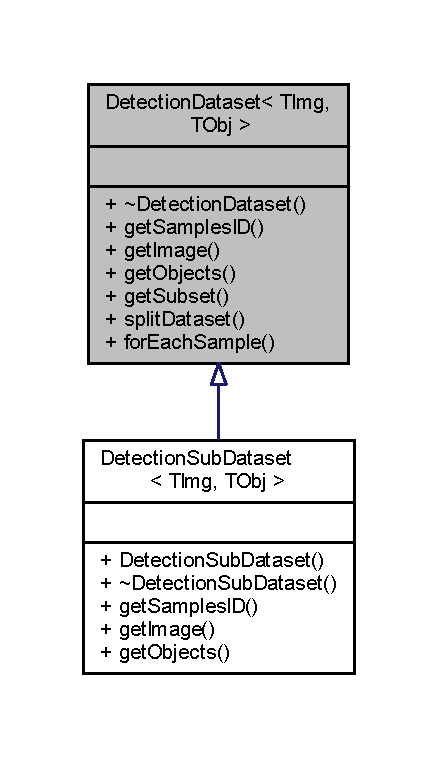
\includegraphics[width=210pt]{class_vision_core_1_1_evaluation_1_1_detection_dataset__inherit__graph}
\end{center}
\end{figure}


Collaboration diagram for Detection\+Dataset$<$ T\+Img, T\+Obj $>$\+:
\nopagebreak
\begin{figure}[H]
\begin{center}
\leavevmode
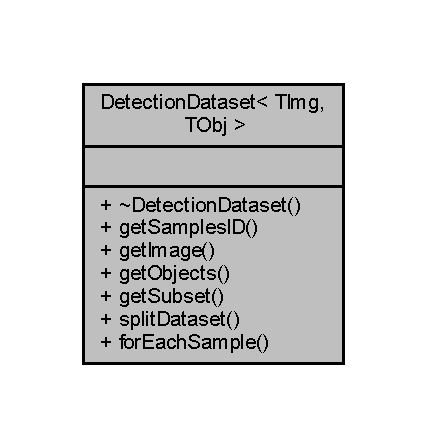
\includegraphics[width=205pt]{class_vision_core_1_1_evaluation_1_1_detection_dataset__coll__graph}
\end{center}
\end{figure}
\subsection*{Public Types}
\begin{DoxyCompactItemize}
\item 
\hypertarget{class_vision_core_1_1_evaluation_1_1_detection_dataset_aaafe8051ac78bd4d8ed3027acd24a1c0}{}typedef T\+Img {\bfseries Img\+Type}\label{class_vision_core_1_1_evaluation_1_1_detection_dataset_aaafe8051ac78bd4d8ed3027acd24a1c0}

\item 
\hypertarget{class_vision_core_1_1_evaluation_1_1_detection_dataset_a34f8ad85716743523e520af46032716e}{}typedef T\+Obj {\bfseries Obj\+Type}\label{class_vision_core_1_1_evaluation_1_1_detection_dataset_a34f8ad85716743523e520af46032716e}

\end{DoxyCompactItemize}
\subsection*{Public Member Functions}
\begin{DoxyCompactItemize}
\item 
\hypertarget{class_vision_core_1_1_evaluation_1_1_detection_dataset_a74f581b470028b781e9f4d6c2e0f56b0}{}virtual \hyperlink{class_vision_core_1_1_evaluation_1_1_detection_dataset_a74f581b470028b781e9f4d6c2e0f56b0}{$\sim$\+Detection\+Dataset} ()\label{class_vision_core_1_1_evaluation_1_1_detection_dataset_a74f581b470028b781e9f4d6c2e0f56b0}

\begin{DoxyCompactList}\small\item\em Destructor method. \end{DoxyCompactList}\item 
\hypertarget{class_vision_core_1_1_evaluation_1_1_detection_dataset_a4baafaba65ce3ae8e9fc8a5f74f5e0f8}{}virtual std\+::vector$<$ std\+::string $>$ \hyperlink{class_vision_core_1_1_evaluation_1_1_detection_dataset_a4baafaba65ce3ae8e9fc8a5f74f5e0f8}{get\+Samples\+I\+D} () const  =0\label{class_vision_core_1_1_evaluation_1_1_detection_dataset_a4baafaba65ce3ae8e9fc8a5f74f5e0f8}

\begin{DoxyCompactList}\small\item\em Returns a vector of I\+Ds for all samples in the dataset. Each sample should be identified by a unique string I\+D. This I\+D can be anything (a number, the name of file, etc). It is used mainly to retrieve a sample through function get\+Image and get\+Objects. \end{DoxyCompactList}\item 
virtual std\+::shared\+\_\+ptr$<$ T\+Img $>$ \hyperlink{class_vision_core_1_1_evaluation_1_1_detection_dataset_afaca4ebdf527646b545947fd4c2ec73c}{get\+Image} (const std\+::string \&sample\+I\+D) const  =0
\begin{DoxyCompactList}\small\item\em Returns a pointer to one of the images in the dataset. \end{DoxyCompactList}\item 
virtual std\+::vector$<$ T\+Obj $>$ \hyperlink{class_vision_core_1_1_evaluation_1_1_detection_dataset_a831ba73d31b15e00777727f98cf23669}{get\+Objects} (const std\+::string \&sample\+I\+D) const  =0
\begin{DoxyCompactList}\small\item\em Returns a vector of objects contained in a sample. This could be a vector of all the faces that appear on a image when working with a face dataset. \end{DoxyCompactList}\item 
\hypertarget{class_vision_core_1_1_evaluation_1_1_detection_dataset_ac21371d93712c4f10a2c44530f402a25}{}\hyperlink{class_vision_core_1_1_evaluation_1_1_detection_sub_dataset}{Detection\+Sub\+Dataset}$<$ T\+Img, T\+Obj $>$ \hyperlink{class_vision_core_1_1_evaluation_1_1_detection_dataset_ac21371d93712c4f10a2c44530f402a25}{get\+Subset} (std\+::vector$<$ std\+::string $>$ samples\+I\+D)\label{class_vision_core_1_1_evaluation_1_1_detection_dataset_ac21371d93712c4f10a2c44530f402a25}

\begin{DoxyCompactList}\small\item\em Returns a dataset containing a subset of samples. The vector samples\+I\+D specify the subset samples. If some sample\+I\+D does not exist in the original dataset an exception is throw. The subset mantains a reference to the original dataset, so the subset is only accessible on the scope of the original dataset. \end{DoxyCompactList}\item 
\hypertarget{class_vision_core_1_1_evaluation_1_1_detection_dataset_a4703b31fbe4c89baf44dfeeb7f2bb18d}{}std\+::vector$<$ \hyperlink{class_vision_core_1_1_evaluation_1_1_detection_sub_dataset}{Detection\+Sub\+Dataset}$<$ T\+Img, T\+Obj $>$ $>$ \hyperlink{class_vision_core_1_1_evaluation_1_1_detection_dataset_a4703b31fbe4c89baf44dfeeb7f2bb18d}{split\+Dataset} (std\+::vector$<$ double $>$ proportions)\label{class_vision_core_1_1_evaluation_1_1_detection_dataset_a4703b31fbe4c89baf44dfeeb7f2bb18d}

\begin{DoxyCompactList}\small\item\em Splits the dataset in several subdatasets according to proportions (must sum to 1). \end{DoxyCompactList}\item 
virtual void \hyperlink{class_vision_core_1_1_evaluation_1_1_detection_dataset_af6f37eeccc1f47bbe5ec0e38199ca8bf}{for\+Each\+Sample} (std\+::function$<$ void(T\+Img \&, std\+::vector$<$ T\+Obj $>$ \&, std\+::string \&)$>$ funct)
\begin{DoxyCompactList}\small\item\em For each sample in dataset execute a function. \end{DoxyCompactList}\end{DoxyCompactItemize}


\subsection{Detailed Description}
\subsubsection*{template$<$class T\+Img, typename T\+Obj$>$class Vision\+Core\+::\+Evaluation\+::\+Detection\+Dataset$<$ T\+Img, T\+Obj $>$}

Abstract class for a generic detection dataset, contining images and its ground-\/truth. 

Each sample in the dataset has an image and a vector of objects considered as ground-\/truth.

Each sample has an unique I\+D. A vector with all samples I\+Ds can be retrieved by method \textquotesingle{}\hyperlink{class_vision_core_1_1_evaluation_1_1_detection_dataset_a4baafaba65ce3ae8e9fc8a5f74f5e0f8}{get\+Samples\+I\+D()}\textquotesingle{}.

The \textquotesingle{}get\+Image(sample\+I\+D)\textquotesingle{} method returns one image from the dataset and the \textquotesingle{}get\+Objects(sample\+I\+D)\textquotesingle{} method returns the respective ground-\/truth objects.

Derived classes implementing this interface must implement the three methods mentioned above.


\begin{DoxyParams}{Parameters}
{\em T\+Img} & Image type. \\
\hline
{\em T\+Obj} & Detected object type. \\
\hline
\end{DoxyParams}


Definition at line 71 of file Vision\+Evaluation.\+h.



\subsection{Member Function Documentation}
\hypertarget{class_vision_core_1_1_evaluation_1_1_detection_dataset_af6f37eeccc1f47bbe5ec0e38199ca8bf}{}\index{Vision\+Core\+::\+Evaluation\+::\+Detection\+Dataset@{Vision\+Core\+::\+Evaluation\+::\+Detection\+Dataset}!for\+Each\+Sample@{for\+Each\+Sample}}
\index{for\+Each\+Sample@{for\+Each\+Sample}!Vision\+Core\+::\+Evaluation\+::\+Detection\+Dataset@{Vision\+Core\+::\+Evaluation\+::\+Detection\+Dataset}}
\subsubsection[{for\+Each\+Sample(std\+::function$<$ void(\+T\+Img \&, std\+::vector$<$ T\+Obj $>$ \&, std\+::string \&)$>$ funct)}]{\setlength{\rightskip}{0pt plus 5cm}void for\+Each\+Sample (
\begin{DoxyParamCaption}
\item[{std\+::function$<$ void(T\+Img \&, std\+::vector$<$ T\+Obj $>$ \&, std\+::string \&)$>$}]{funct}
\end{DoxyParamCaption}
)\hspace{0.3cm}{\ttfamily [virtual]}}\label{class_vision_core_1_1_evaluation_1_1_detection_dataset_af6f37eeccc1f47bbe5ec0e38199ca8bf}


For each sample in dataset execute a function. 


\begin{DoxyParams}{Parameters}
{\em T\+Img} & Image type \\
\hline
{\em T\+Obj} & Object type of the ground truth annotations. \\
\hline
{\em funct} & A function that will be execute for each sample in the dataset. \\
\hline
\end{DoxyParams}


Definition at line 113 of file Vision\+Evaluation.\+h.



Here is the caller graph for this function\+:
\nopagebreak
\begin{figure}[H]
\begin{center}
\leavevmode
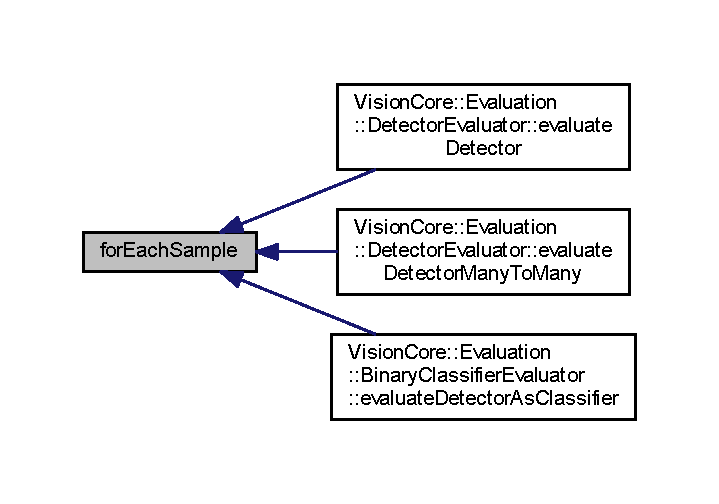
\includegraphics[width=345pt]{class_vision_core_1_1_evaluation_1_1_detection_dataset_af6f37eeccc1f47bbe5ec0e38199ca8bf_icgraph}
\end{center}
\end{figure}


\hypertarget{class_vision_core_1_1_evaluation_1_1_detection_dataset_afaca4ebdf527646b545947fd4c2ec73c}{}\index{Vision\+Core\+::\+Evaluation\+::\+Detection\+Dataset@{Vision\+Core\+::\+Evaluation\+::\+Detection\+Dataset}!get\+Image@{get\+Image}}
\index{get\+Image@{get\+Image}!Vision\+Core\+::\+Evaluation\+::\+Detection\+Dataset@{Vision\+Core\+::\+Evaluation\+::\+Detection\+Dataset}}
\subsubsection[{get\+Image(const std\+::string \&sample\+I\+D) const  =0}]{\setlength{\rightskip}{0pt plus 5cm}virtual std\+::shared\+\_\+ptr$<$T\+Img$>$ get\+Image (
\begin{DoxyParamCaption}
\item[{const std\+::string \&}]{sample\+I\+D}
\end{DoxyParamCaption}
) const\hspace{0.3cm}{\ttfamily [pure virtual]}}\label{class_vision_core_1_1_evaluation_1_1_detection_dataset_afaca4ebdf527646b545947fd4c2ec73c}


Returns a pointer to one of the images in the dataset. 


\begin{DoxyParams}{Parameters}
{\em sample\+I\+D} & The unique identifier for the sample you are fetching. \\
\hline
\end{DoxyParams}


Implemented in \hyperlink{class_vision_core_1_1_evaluation_1_1_detection_sub_dataset_a8d5c26c8bba720739540caea9cd2f630}{Detection\+Sub\+Dataset$<$ T\+Img, T\+Obj $>$}, and \hyperlink{class_viscv_1_1_dataset_f_d_d_b_a64f0340b5a377d18c5199f61a8ee7ffd}{Dataset\+F\+D\+D\+B}.

\hypertarget{class_vision_core_1_1_evaluation_1_1_detection_dataset_a831ba73d31b15e00777727f98cf23669}{}\index{Vision\+Core\+::\+Evaluation\+::\+Detection\+Dataset@{Vision\+Core\+::\+Evaluation\+::\+Detection\+Dataset}!get\+Objects@{get\+Objects}}
\index{get\+Objects@{get\+Objects}!Vision\+Core\+::\+Evaluation\+::\+Detection\+Dataset@{Vision\+Core\+::\+Evaluation\+::\+Detection\+Dataset}}
\subsubsection[{get\+Objects(const std\+::string \&sample\+I\+D) const  =0}]{\setlength{\rightskip}{0pt plus 5cm}virtual std\+::vector$<$T\+Obj$>$ get\+Objects (
\begin{DoxyParamCaption}
\item[{const std\+::string \&}]{sample\+I\+D}
\end{DoxyParamCaption}
) const\hspace{0.3cm}{\ttfamily [pure virtual]}}\label{class_vision_core_1_1_evaluation_1_1_detection_dataset_a831ba73d31b15e00777727f98cf23669}


Returns a vector of objects contained in a sample. This could be a vector of all the faces that appear on a image when working with a face dataset. 


\begin{DoxyParams}{Parameters}
{\em sample\+I\+D} & The unique identifier for the sample you are fetching. \\
\hline
\end{DoxyParams}


Implemented in \hyperlink{class_vision_core_1_1_evaluation_1_1_detection_sub_dataset_a4c1bd88038f81317438d052bcbf2bfaa}{Detection\+Sub\+Dataset$<$ T\+Img, T\+Obj $>$}, and \hyperlink{class_viscv_1_1_dataset_f_d_d_b_a8c1fe796c01ff8d85626dd85e6a45418}{Dataset\+F\+D\+D\+B}.



The documentation for this class was generated from the following file\+:\begin{DoxyCompactItemize}
\item 
D\+:/\+F\+U\+R\+G/\+Software/\+Cv\+Works\+Release1/\+Core/\+Vision/Vision\+Evaluation.\+h\end{DoxyCompactItemize}

\hypertarget{class_detection_dataset_control}{}\section{Detection\+Dataset\+Control$<$ T\+Obj $>$ Class Template Reference}
\label{class_detection_dataset_control}\index{Detection\+Dataset\+Control$<$ T\+Obj $>$@{Detection\+Dataset\+Control$<$ T\+Obj $>$}}


Inheritance diagram for Detection\+Dataset\+Control$<$ T\+Obj $>$\+:
\nopagebreak
\begin{figure}[H]
\begin{center}
\leavevmode
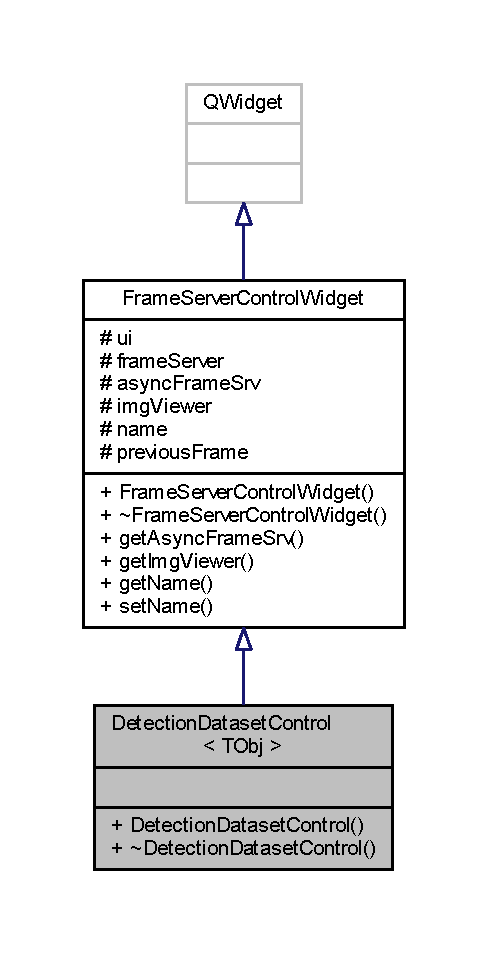
\includegraphics[width=234pt]{class_detection_dataset_control__inherit__graph}
\end{center}
\end{figure}


Collaboration diagram for Detection\+Dataset\+Control$<$ T\+Obj $>$\+:
\nopagebreak
\begin{figure}[H]
\begin{center}
\leavevmode
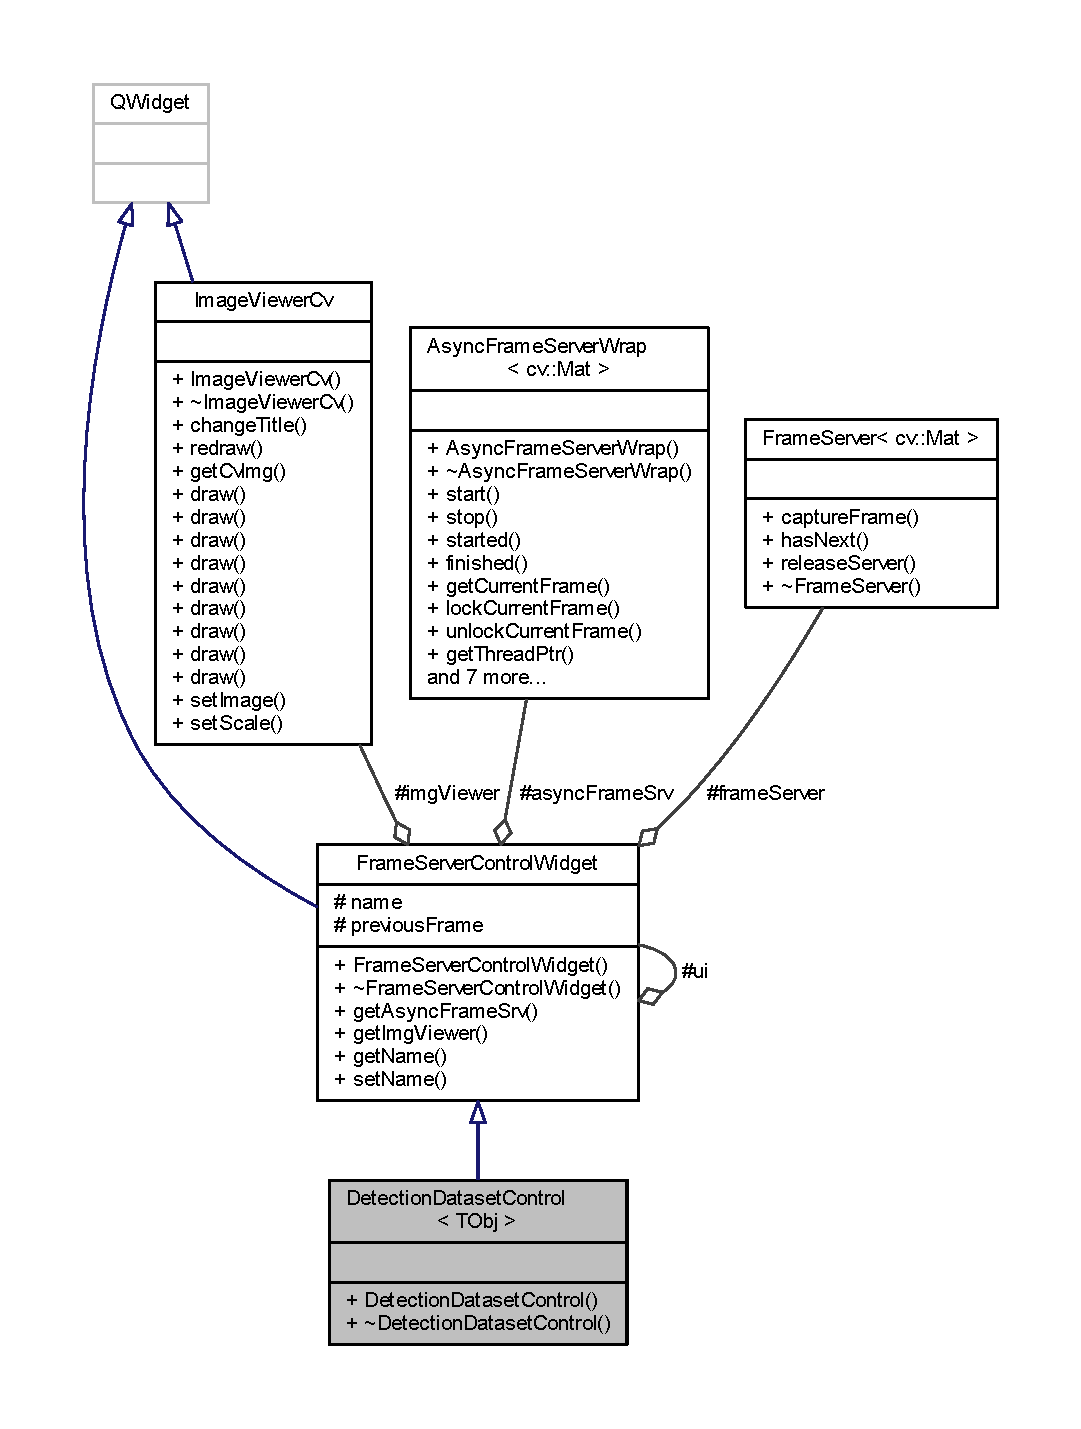
\includegraphics[width=350pt]{class_detection_dataset_control__coll__graph}
\end{center}
\end{figure}
\subsection*{Public Member Functions}
\begin{DoxyCompactItemize}
\item 
\hypertarget{class_detection_dataset_control_a9fd1de3909b08bbf725de0f0156fe41c}{}{\bfseries Detection\+Dataset\+Control} (\hyperlink{class_vision_core_1_1_evaluation_1_1_detection_dataset}{Vision\+Core\+::\+Detection\+Dataset}$<$ cv\+::\+Mat, T\+Obj $>$ $\ast$det\+Data)\label{class_detection_dataset_control_a9fd1de3909b08bbf725de0f0156fe41c}

\end{DoxyCompactItemize}
\subsection*{Additional Inherited Members}


\subsection{Detailed Description}
\subsubsection*{template$<$class T\+Obj$>$class Detection\+Dataset\+Control$<$ T\+Obj $>$}



Definition at line 45 of file Detection\+Dataset\+Control.\+h.



The documentation for this class was generated from the following file\+:\begin{DoxyCompactItemize}
\item 
D\+:/\+F\+U\+R\+G/\+Software/\+Cv\+Works\+Release1/\+Applications/\+Vision\+G\+U\+I/Detection\+Dataset\+Control.\+h\end{DoxyCompactItemize}

\hypertarget{class_vision_core_1_1_evaluation_1_1_detection_sub_dataset}{}\section{Detection\+Sub\+Dataset$<$ T\+Img, T\+Obj $>$ Class Template Reference}
\label{class_vision_core_1_1_evaluation_1_1_detection_sub_dataset}\index{Detection\+Sub\+Dataset$<$ T\+Img, T\+Obj $>$@{Detection\+Sub\+Dataset$<$ T\+Img, T\+Obj $>$}}


Class that provides access to a subset of a detection dataset.  




{\ttfamily \#include $<$Vision\+Evaluation.\+h$>$}



Inheritance diagram for Detection\+Sub\+Dataset$<$ T\+Img, T\+Obj $>$\+:
\nopagebreak
\begin{figure}[H]
\begin{center}
\leavevmode
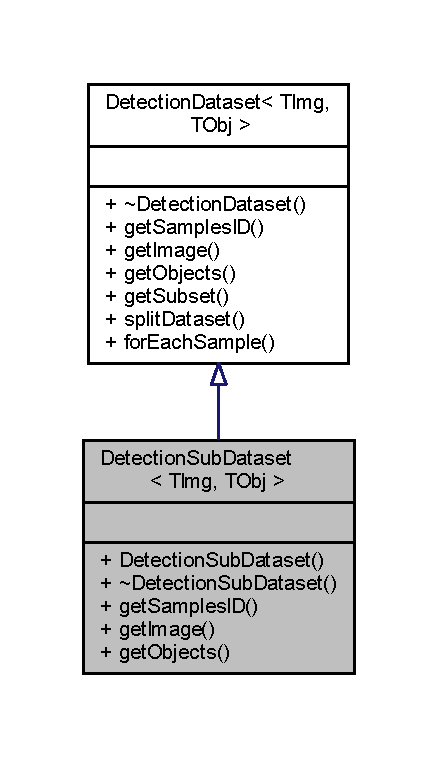
\includegraphics[width=210pt]{class_vision_core_1_1_evaluation_1_1_detection_sub_dataset__inherit__graph}
\end{center}
\end{figure}


Collaboration diagram for Detection\+Sub\+Dataset$<$ T\+Img, T\+Obj $>$\+:
\nopagebreak
\begin{figure}[H]
\begin{center}
\leavevmode
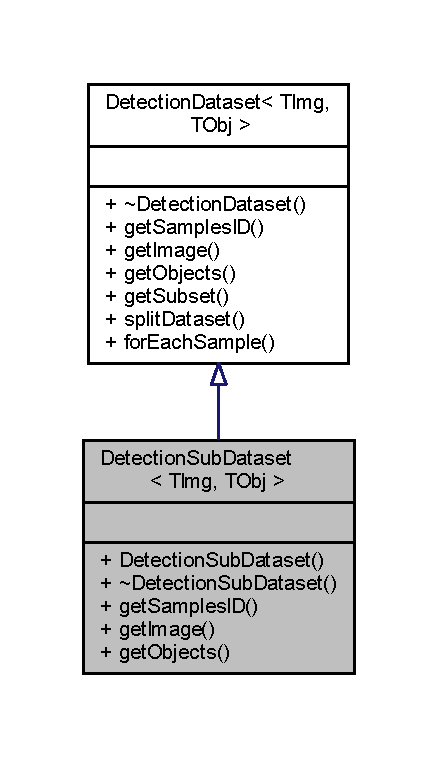
\includegraphics[width=210pt]{class_vision_core_1_1_evaluation_1_1_detection_sub_dataset__coll__graph}
\end{center}
\end{figure}
\subsection*{Public Member Functions}
\begin{DoxyCompactItemize}
\item 
\hypertarget{class_vision_core_1_1_evaluation_1_1_detection_sub_dataset_a4acd269a8a0ec8b613b30500751444df}{}\hyperlink{class_vision_core_1_1_evaluation_1_1_detection_sub_dataset_a4acd269a8a0ec8b613b30500751444df}{Detection\+Sub\+Dataset} (\hyperlink{class_vision_core_1_1_evaluation_1_1_detection_dataset}{Detection\+Dataset}$<$ T\+Img, T\+Obj $>$ \&dataset\+\_\+, const std\+::vector$<$ unsigned int $>$ \&samples\+Number\+\_\+)\label{class_vision_core_1_1_evaluation_1_1_detection_sub_dataset_a4acd269a8a0ec8b613b30500751444df}

\begin{DoxyCompactList}\small\item\em Constructructor. \end{DoxyCompactList}\item 
\hypertarget{class_vision_core_1_1_evaluation_1_1_detection_sub_dataset_a969a20140a15bb8c98e8fa915963a6ce}{}virtual \hyperlink{class_vision_core_1_1_evaluation_1_1_detection_sub_dataset_a969a20140a15bb8c98e8fa915963a6ce}{$\sim$\+Detection\+Sub\+Dataset} ()\label{class_vision_core_1_1_evaluation_1_1_detection_sub_dataset_a969a20140a15bb8c98e8fa915963a6ce}

\begin{DoxyCompactList}\small\item\em Destructor method. \end{DoxyCompactList}\item 
virtual std\+::vector$<$ std\+::string $>$ \hyperlink{class_vision_core_1_1_evaluation_1_1_detection_sub_dataset_a8f2602813f5b8c2c6512690efbabb2df}{get\+Samples\+I\+D} () const 
\begin{DoxyCompactList}\small\item\em Returns a vector of I\+Ds for all samples in the dataset. Each sample should be identified by a unique string I\+D. This I\+D can be anything (a number, the name of file, etc). It is used mainly to retrieve a sample through function get\+Image and get\+Objects. \end{DoxyCompactList}\item 
virtual std\+::shared\+\_\+ptr$<$ T\+Img $>$ \hyperlink{class_vision_core_1_1_evaluation_1_1_detection_sub_dataset_a8d5c26c8bba720739540caea9cd2f630}{get\+Image} (const std\+::string \&sample\+I\+D) const 
\begin{DoxyCompactList}\small\item\em Returns a pointer to one of the images in the dataset. \end{DoxyCompactList}\item 
virtual std\+::vector$<$ T\+Obj $>$ \hyperlink{class_vision_core_1_1_evaluation_1_1_detection_sub_dataset_a4c1bd88038f81317438d052bcbf2bfaa}{get\+Objects} (const std\+::string \&sample\+I\+D) const 
\begin{DoxyCompactList}\small\item\em Returns a vector of objects contained in a sample. This could be a vector of all the faces that appear on a image when working with a face dataset. \end{DoxyCompactList}\end{DoxyCompactItemize}
\subsection*{Additional Inherited Members}


\subsection{Detailed Description}
\subsubsection*{template$<$class T\+Img, typename T\+Obj$>$class Vision\+Core\+::\+Evaluation\+::\+Detection\+Sub\+Dataset$<$ T\+Img, T\+Obj $>$}

Class that provides access to a subset of a detection dataset. 

This class provides access to only a subset of samples from a original dataset. The original dataset is stored as a reference, so the subset is only accessible on the scope of the original dataset. The identification of which samples compose the subset is passed on constructor as a vector of samples number or samples I\+D. 
\begin{DoxyParams}{Parameters}
{\em T\+Img} & Image type. \\
\hline
{\em T\+Obj} & Detected object type. \\
\hline
\end{DoxyParams}


Definition at line 53 of file Vision\+Evaluation.\+h.



\subsection{Member Function Documentation}
\hypertarget{class_vision_core_1_1_evaluation_1_1_detection_sub_dataset_a8d5c26c8bba720739540caea9cd2f630}{}\index{Vision\+Core\+::\+Evaluation\+::\+Detection\+Sub\+Dataset@{Vision\+Core\+::\+Evaluation\+::\+Detection\+Sub\+Dataset}!get\+Image@{get\+Image}}
\index{get\+Image@{get\+Image}!Vision\+Core\+::\+Evaluation\+::\+Detection\+Sub\+Dataset@{Vision\+Core\+::\+Evaluation\+::\+Detection\+Sub\+Dataset}}
\subsubsection[{get\+Image(const std\+::string \&sample\+I\+D) const }]{\setlength{\rightskip}{0pt plus 5cm}std\+::shared\+\_\+ptr$<$ T\+Img $>$ get\+Image (
\begin{DoxyParamCaption}
\item[{const std\+::string \&}]{sample\+I\+D}
\end{DoxyParamCaption}
) const\hspace{0.3cm}{\ttfamily [virtual]}}\label{class_vision_core_1_1_evaluation_1_1_detection_sub_dataset_a8d5c26c8bba720739540caea9cd2f630}


Returns a pointer to one of the images in the dataset. 


\begin{DoxyParams}{Parameters}
{\em sample\+I\+D} & The unique identifier for the sample you are fetching. \\
\hline
\end{DoxyParams}


Implements \hyperlink{class_vision_core_1_1_evaluation_1_1_detection_dataset_afaca4ebdf527646b545947fd4c2ec73c}{Detection\+Dataset$<$ T\+Img, T\+Obj $>$}.



Definition at line 203 of file Vision\+Evaluation.\+h.

\hypertarget{class_vision_core_1_1_evaluation_1_1_detection_sub_dataset_a4c1bd88038f81317438d052bcbf2bfaa}{}\index{Vision\+Core\+::\+Evaluation\+::\+Detection\+Sub\+Dataset@{Vision\+Core\+::\+Evaluation\+::\+Detection\+Sub\+Dataset}!get\+Objects@{get\+Objects}}
\index{get\+Objects@{get\+Objects}!Vision\+Core\+::\+Evaluation\+::\+Detection\+Sub\+Dataset@{Vision\+Core\+::\+Evaluation\+::\+Detection\+Sub\+Dataset}}
\subsubsection[{get\+Objects(const std\+::string \&sample\+I\+D) const }]{\setlength{\rightskip}{0pt plus 5cm}std\+::vector$<$ T\+Obj $>$ get\+Objects (
\begin{DoxyParamCaption}
\item[{const std\+::string \&}]{sample\+I\+D}
\end{DoxyParamCaption}
) const\hspace{0.3cm}{\ttfamily [virtual]}}\label{class_vision_core_1_1_evaluation_1_1_detection_sub_dataset_a4c1bd88038f81317438d052bcbf2bfaa}


Returns a vector of objects contained in a sample. This could be a vector of all the faces that appear on a image when working with a face dataset. 


\begin{DoxyParams}{Parameters}
{\em sample\+I\+D} & The unique identifier for the sample you are fetching. \\
\hline
\end{DoxyParams}


Implements \hyperlink{class_vision_core_1_1_evaluation_1_1_detection_dataset_a831ba73d31b15e00777727f98cf23669}{Detection\+Dataset$<$ T\+Img, T\+Obj $>$}.



Definition at line 209 of file Vision\+Evaluation.\+h.

\hypertarget{class_vision_core_1_1_evaluation_1_1_detection_sub_dataset_a8f2602813f5b8c2c6512690efbabb2df}{}\index{Vision\+Core\+::\+Evaluation\+::\+Detection\+Sub\+Dataset@{Vision\+Core\+::\+Evaluation\+::\+Detection\+Sub\+Dataset}!get\+Samples\+I\+D@{get\+Samples\+I\+D}}
\index{get\+Samples\+I\+D@{get\+Samples\+I\+D}!Vision\+Core\+::\+Evaluation\+::\+Detection\+Sub\+Dataset@{Vision\+Core\+::\+Evaluation\+::\+Detection\+Sub\+Dataset}}
\subsubsection[{get\+Samples\+I\+D() const }]{\setlength{\rightskip}{0pt plus 5cm}std\+::vector$<$ std\+::string $>$ get\+Samples\+I\+D (
\begin{DoxyParamCaption}
{}
\end{DoxyParamCaption}
) const\hspace{0.3cm}{\ttfamily [virtual]}}\label{class_vision_core_1_1_evaluation_1_1_detection_sub_dataset_a8f2602813f5b8c2c6512690efbabb2df}


Returns a vector of I\+Ds for all samples in the dataset. Each sample should be identified by a unique string I\+D. This I\+D can be anything (a number, the name of file, etc). It is used mainly to retrieve a sample through function get\+Image and get\+Objects. 

Gets only a subset from the original dataset 

Implements \hyperlink{class_vision_core_1_1_evaluation_1_1_detection_dataset_a4baafaba65ce3ae8e9fc8a5f74f5e0f8}{Detection\+Dataset$<$ T\+Img, T\+Obj $>$}.



Definition at line 191 of file Vision\+Evaluation.\+h.



The documentation for this class was generated from the following file\+:\begin{DoxyCompactItemize}
\item 
D\+:/\+F\+U\+R\+G/\+Software/\+Cv\+Works\+Release1/\+Core/\+Vision/Vision\+Evaluation.\+h\end{DoxyCompactItemize}

\hypertarget{class_vision_core_1_1_interfaces_1_1_detector}{}\section{Detector$<$ T\+Img, T\+Obj $>$ Class Template Reference}
\label{class_vision_core_1_1_interfaces_1_1_detector}\index{Detector$<$ T\+Img, T\+Obj $>$@{Detector$<$ T\+Img, T\+Obj $>$}}


Interface defining a generic object detector (e.\+g. faces, car, people).  




{\ttfamily \#include $<$Vision\+Interfaces.\+h$>$}



Inheritance diagram for Detector$<$ T\+Img, T\+Obj $>$\+:
\nopagebreak
\begin{figure}[H]
\begin{center}
\leavevmode
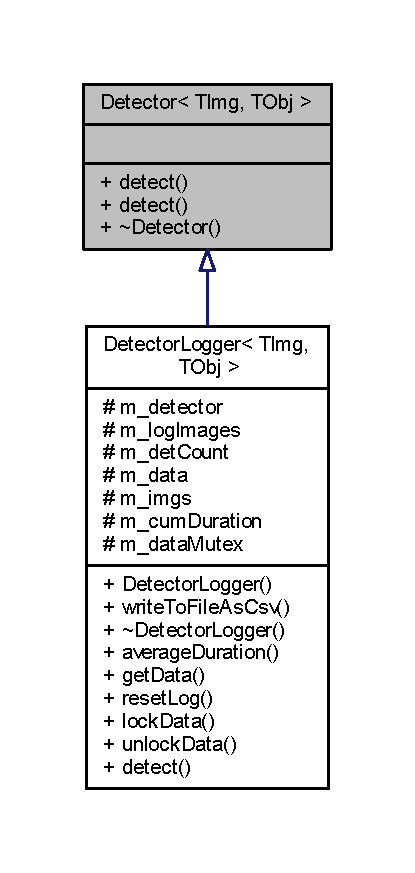
\includegraphics[width=199pt]{class_vision_core_1_1_interfaces_1_1_detector__inherit__graph}
\end{center}
\end{figure}


Collaboration diagram for Detector$<$ T\+Img, T\+Obj $>$\+:
\nopagebreak
\begin{figure}[H]
\begin{center}
\leavevmode
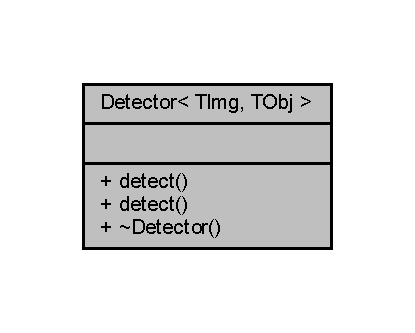
\includegraphics[width=199pt]{class_vision_core_1_1_interfaces_1_1_detector__coll__graph}
\end{center}
\end{figure}
\subsection*{Public Types}
\begin{DoxyCompactItemize}
\item 
\hypertarget{class_vision_core_1_1_interfaces_1_1_detector_aaafe8051ac78bd4d8ed3027acd24a1c0}{}typedef T\+Img {\bfseries Img\+Type}\label{class_vision_core_1_1_interfaces_1_1_detector_aaafe8051ac78bd4d8ed3027acd24a1c0}

\item 
\hypertarget{class_vision_core_1_1_interfaces_1_1_detector_a34f8ad85716743523e520af46032716e}{}typedef T\+Obj {\bfseries Obj\+Type}\label{class_vision_core_1_1_interfaces_1_1_detector_a34f8ad85716743523e520af46032716e}

\end{DoxyCompactItemize}
\subsection*{Public Member Functions}
\begin{DoxyCompactItemize}
\item 
virtual std\+::vector$<$ T\+Obj $>$ \hyperlink{class_vision_core_1_1_interfaces_1_1_detector_a0977745b253f810bb2ec009844618305}{detect} (const T\+Img \&img) const  =0
\begin{DoxyCompactList}\small\item\em Detects objects in the image and returns a vector with the detected objects. \end{DoxyCompactList}\item 
\hypertarget{class_vision_core_1_1_interfaces_1_1_detector_a4e37933b023a5f4d4f28c5b5bf3f9459}{}virtual void {\bfseries detect} (const T\+Img \&img, std\+::vector$<$ T\+Obj $>$ \&obj) const \label{class_vision_core_1_1_interfaces_1_1_detector_a4e37933b023a5f4d4f28c5b5bf3f9459}

\item 
\hypertarget{class_vision_core_1_1_interfaces_1_1_detector_a91a737d10b7440970932af8c8d8380d2}{}virtual \hyperlink{class_vision_core_1_1_interfaces_1_1_detector_a91a737d10b7440970932af8c8d8380d2}{$\sim$\+Detector} ()\label{class_vision_core_1_1_interfaces_1_1_detector_a91a737d10b7440970932af8c8d8380d2}

\begin{DoxyCompactList}\small\item\em Destrutor. \end{DoxyCompactList}\end{DoxyCompactItemize}


\subsection{Detailed Description}
\subsubsection*{template$<$class T\+Img, class T\+Obj$>$class Vision\+Core\+::\+Interfaces\+::\+Detector$<$ T\+Img, T\+Obj $>$}

Interface defining a generic object detector (e.\+g. faces, car, people). 

An object detector, as defined here, is a computer vision method that finds objects in a given image.

Usually, the object position is represented by a bounding rectangle around the object, however other representation can also be used (a bounding circle, the object contour, or simple a point). Some methods can detect not only the position, but also more complex information, like a skeleton for a people detector.

This interface provides a minimal and generic description of an object detector. The interface has only one method\+: \hyperlink{class_vision_core_1_1_interfaces_1_1_detector_a0977745b253f810bb2ec009844618305}{detect()}, which receives an input image and returns a vector of objects found within the image. Both the image and object types are generic.


\begin{DoxyParams}{Parameters}
{\em T\+Img} & Image type used in the detector. \\
\hline
{\em T\+Obj} & Object type returned by the detector. \\
\hline
\end{DoxyParams}
\begin{DoxySeeAlso}{See also}
Async\+Detector\+Wrap Circle\+Detector\+H\+T\+C\+F 
\end{DoxySeeAlso}


Definition at line 125 of file Vision\+Interfaces.\+h.



\subsection{Member Function Documentation}
\hypertarget{class_vision_core_1_1_interfaces_1_1_detector_a0977745b253f810bb2ec009844618305}{}\index{Vision\+Core\+::\+Interfaces\+::\+Detector@{Vision\+Core\+::\+Interfaces\+::\+Detector}!detect@{detect}}
\index{detect@{detect}!Vision\+Core\+::\+Interfaces\+::\+Detector@{Vision\+Core\+::\+Interfaces\+::\+Detector}}
\subsubsection[{detect(const T\+Img \&img) const  =0}]{\setlength{\rightskip}{0pt plus 5cm}virtual std\+::vector$<$T\+Obj$>$ detect (
\begin{DoxyParamCaption}
\item[{const T\+Img \&}]{img}
\end{DoxyParamCaption}
) const\hspace{0.3cm}{\ttfamily [pure virtual]}}\label{class_vision_core_1_1_interfaces_1_1_detector_a0977745b253f810bb2ec009844618305}


Detects objects in the image and returns a vector with the detected objects. 

The vector should be empty if no object is detected. 

Implemented in \hyperlink{class_vision_core_1_1_abstractions_1_1_detector_logger_a1f2edd31854cbaeed7db844d4e5bcbfc}{Detector\+Logger$<$ T\+Img, T\+Obj $>$}, \hyperlink{class_vision_core_1_1_abstractions_1_1_detector_logger_a1f2edd31854cbaeed7db844d4e5bcbfc}{Detector\+Logger$<$ cv\+::\+Mat, cv\+::\+Rect $>$}, \hyperlink{class_viscv_1_1_a_r_tag_detector_b_l_p_a0065a0a0e3dbed236849bf406e6cde66}{A\+R\+Tag\+Detector\+B\+L\+P}, \hyperlink{class_viscv_1_1_object_detector_c_c_cv_a1d0c071b6e7a19b192c86ca0e47fd642}{Object\+Detector\+C\+C\+Cv}, \hyperlink{class_viscv_1_1_circle_detector_h_t_c_f_ad8f008988f0c246f86a192f8c17c3a88}{Circle\+Detector\+H\+T\+C\+F}, \hyperlink{class_viscv_1_1_line_detector_h_t_a8128bf0deed5f697117c5948fc7c014d}{Line\+Detector\+H\+T}, \hyperlink{class_viscv_1_1_color_blob_detector_h_f_a76311b08b5cb9df65524e070e9c15048}{Color\+Blob\+Detector\+H\+F}, \hyperlink{class_viscv_1_1_templ_matching_detector_a1d0c071b6e7a19b192c86ca0e47fd642}{Templ\+Matching\+Detector}, and \hyperlink{class_viscv_1_1_object_detector_f_m_cv_a1d0c071b6e7a19b192c86ca0e47fd642}{Object\+Detector\+F\+M\+Cv}.



Here is the caller graph for this function\+:
\nopagebreak
\begin{figure}[H]
\begin{center}
\leavevmode
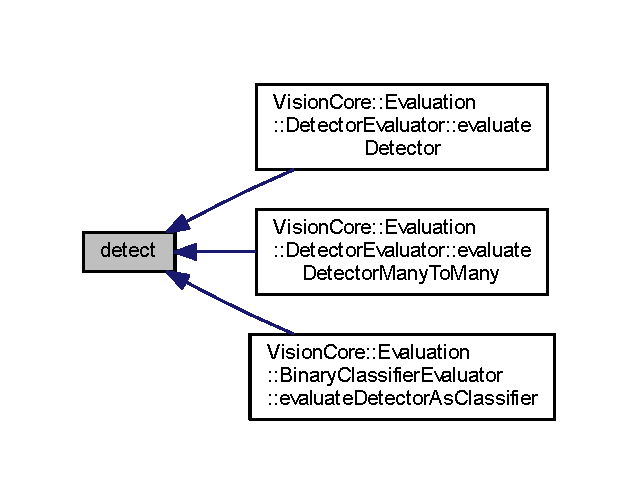
\includegraphics[width=306pt]{class_vision_core_1_1_interfaces_1_1_detector_a0977745b253f810bb2ec009844618305_icgraph}
\end{center}
\end{figure}




The documentation for this class was generated from the following file\+:\begin{DoxyCompactItemize}
\item 
D\+:/\+F\+U\+R\+G/\+Software/\+Cv\+Works\+Release1/\+Core/\+Vision/Vision\+Interfaces.\+h\end{DoxyCompactItemize}

\hypertarget{class_vision_core_1_1_abstractions_1_1_detector_based_multi_tracker}{}\section{Detector\+Based\+Multi\+Tracker$<$ T\+Img, T\+Obj $>$ Class Template Reference}
\label{class_vision_core_1_1_abstractions_1_1_detector_based_multi_tracker}\index{Detector\+Based\+Multi\+Tracker$<$ T\+Img, T\+Obj $>$@{Detector\+Based\+Multi\+Tracker$<$ T\+Img, T\+Obj $>$}}


A tracker that applies a detector on every frame.  




{\ttfamily \#include $<$Vision\+Abstractions.\+h$>$}



Inheritance diagram for Detector\+Based\+Multi\+Tracker$<$ T\+Img, T\+Obj $>$\+:
\nopagebreak
\begin{figure}[H]
\begin{center}
\leavevmode
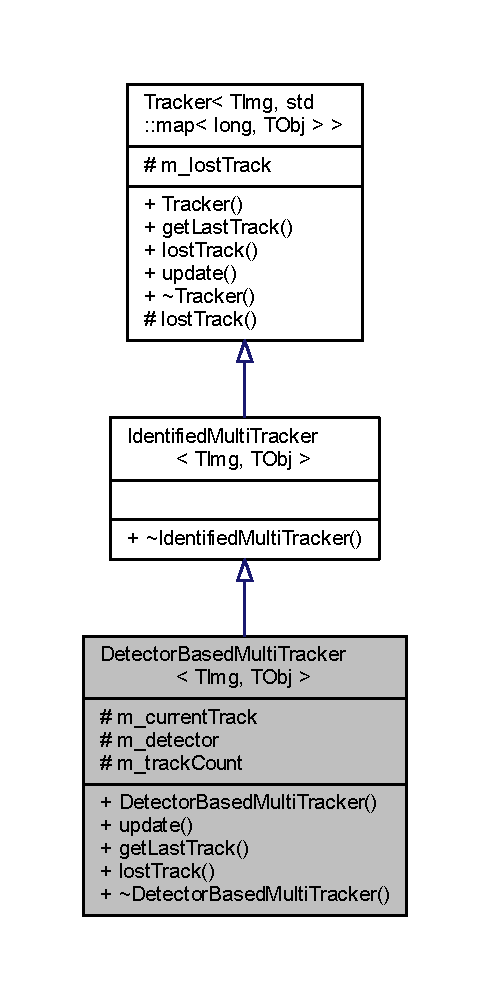
\includegraphics[width=235pt]{class_vision_core_1_1_abstractions_1_1_detector_based_multi_tracker__inherit__graph}
\end{center}
\end{figure}


Collaboration diagram for Detector\+Based\+Multi\+Tracker$<$ T\+Img, T\+Obj $>$\+:
\nopagebreak
\begin{figure}[H]
\begin{center}
\leavevmode
\includegraphics[width=333pt]{class_vision_core_1_1_abstractions_1_1_detector_based_multi_tracker__coll__graph}
\end{center}
\end{figure}
\subsection*{Public Member Functions}
\begin{DoxyCompactItemize}
\item 
\hypertarget{class_vision_core_1_1_abstractions_1_1_detector_based_multi_tracker_a1a1d90f1a87b6b645974c711686c14da}{}\hyperlink{class_vision_core_1_1_abstractions_1_1_detector_based_multi_tracker_a1a1d90f1a87b6b645974c711686c14da}{Detector\+Based\+Multi\+Tracker} (\hyperlink{class_vision_core_1_1_interfaces_1_1_detector}{Detector}$<$ T\+Img, T\+Obj $>$ $\ast$detector)\label{class_vision_core_1_1_abstractions_1_1_detector_based_multi_tracker_a1a1d90f1a87b6b645974c711686c14da}

\begin{DoxyCompactList}\small\item\em Constructor method. \end{DoxyCompactList}\item 
\hypertarget{class_vision_core_1_1_abstractions_1_1_detector_based_multi_tracker_af1a54610c9af7fb54d00e4be2e75609e}{}void \hyperlink{class_vision_core_1_1_abstractions_1_1_detector_based_multi_tracker_af1a54610c9af7fb54d00e4be2e75609e}{update} (const \hyperlink{struct_vision_core_1_1_data_structures_1_1_frame}{Frame}$<$ T\+Img $>$ \&frame)\label{class_vision_core_1_1_abstractions_1_1_detector_based_multi_tracker_af1a54610c9af7fb54d00e4be2e75609e}

\begin{DoxyCompactList}\small\item\em Given an image (i.\+e. video frame), update the tracked object. \end{DoxyCompactList}\item 
const std\+::map$<$ long, T\+Obj $>$ \& \hyperlink{class_vision_core_1_1_abstractions_1_1_detector_based_multi_tracker_a9c8e82bfdf34a35ef2eee54006181e5b}{get\+Last\+Track} ()
\begin{DoxyCompactList}\small\item\em Returns a reference to the current estimated object state. \end{DoxyCompactList}\item 
bool \hyperlink{class_vision_core_1_1_abstractions_1_1_detector_based_multi_tracker_ac7e0977fa702f98038bbe303df458a6c}{lost\+Track} () const 
\begin{DoxyCompactList}\small\item\em Returns true if the tracker lost the object track. \end{DoxyCompactList}\item 
\hypertarget{class_vision_core_1_1_abstractions_1_1_detector_based_multi_tracker_ab6f751b645585a462d8d2faa6edfbd44}{}virtual \hyperlink{class_vision_core_1_1_abstractions_1_1_detector_based_multi_tracker_ab6f751b645585a462d8d2faa6edfbd44}{$\sim$\+Detector\+Based\+Multi\+Tracker} ()\label{class_vision_core_1_1_abstractions_1_1_detector_based_multi_tracker_ab6f751b645585a462d8d2faa6edfbd44}

\begin{DoxyCompactList}\small\item\em Destructor method. \end{DoxyCompactList}\end{DoxyCompactItemize}
\subsection*{Protected Attributes}
\begin{DoxyCompactItemize}
\item 
\hypertarget{class_vision_core_1_1_abstractions_1_1_detector_based_multi_tracker_a0e0f9bebf9bf7ec1ff1bbac02ad9cca1}{}std\+::map$<$ long, T\+Obj $>$ \hyperlink{class_vision_core_1_1_abstractions_1_1_detector_based_multi_tracker_a0e0f9bebf9bf7ec1ff1bbac02ad9cca1}{m\+\_\+current\+Track}\label{class_vision_core_1_1_abstractions_1_1_detector_based_multi_tracker_a0e0f9bebf9bf7ec1ff1bbac02ad9cca1}

\begin{DoxyCompactList}\small\item\em Stores the current tracked objects. Returned by method \hyperlink{class_vision_core_1_1_abstractions_1_1_detector_based_multi_tracker_a9c8e82bfdf34a35ef2eee54006181e5b}{get\+Last\+Track()}. \end{DoxyCompactList}\item 
\hypertarget{class_vision_core_1_1_abstractions_1_1_detector_based_multi_tracker_a5e56e46f08984f7e62a33e0bf4bb057d}{}\hyperlink{class_vision_core_1_1_interfaces_1_1_detector}{Detector}$<$ T\+Img, T\+Obj $>$ $\ast$ \hyperlink{class_vision_core_1_1_abstractions_1_1_detector_based_multi_tracker_a5e56e46f08984f7e62a33e0bf4bb057d}{m\+\_\+detector}\label{class_vision_core_1_1_abstractions_1_1_detector_based_multi_tracker_a5e56e46f08984f7e62a33e0bf4bb057d}

\begin{DoxyCompactList}\small\item\em Detector used on every frame. \end{DoxyCompactList}\item 
\hypertarget{class_vision_core_1_1_abstractions_1_1_detector_based_multi_tracker_a1ac65c40264a42b7c9af36bb470fcc3a}{}long \hyperlink{class_vision_core_1_1_abstractions_1_1_detector_based_multi_tracker_a1ac65c40264a42b7c9af36bb470fcc3a}{m\+\_\+track\+Count}\label{class_vision_core_1_1_abstractions_1_1_detector_based_multi_tracker_a1ac65c40264a42b7c9af36bb470fcc3a}

\begin{DoxyCompactList}\small\item\em Internal counter for identifying new tracked objects. \end{DoxyCompactList}\end{DoxyCompactItemize}
\subsection*{Additional Inherited Members}


\subsection{Detailed Description}
\subsubsection*{template$<$class T\+Img, class T\+Obj$>$class Vision\+Core\+::\+Abstractions\+::\+Detector\+Based\+Multi\+Tracker$<$ T\+Img, T\+Obj $>$}

A tracker that applies a detector on every frame. 

This tracker does a full detection on every frame and match each detected object with the currently tracked objects.

If a detected object is not matched with a current tracked object it is assumed that it is a new object and, therefore, it is added to the tracked objects. On the other hand, if a currently tracked object is not detected in the frame, it is removed from tracked objects.

The Hungarian algorithm is applied to match detected and tracked objects. 

Definition at line 319 of file Vision\+Abstractions.\+h.



\subsection{Member Function Documentation}
\hypertarget{class_vision_core_1_1_abstractions_1_1_detector_based_multi_tracker_a9c8e82bfdf34a35ef2eee54006181e5b}{}\index{Vision\+Core\+::\+Abstractions\+::\+Detector\+Based\+Multi\+Tracker@{Vision\+Core\+::\+Abstractions\+::\+Detector\+Based\+Multi\+Tracker}!get\+Last\+Track@{get\+Last\+Track}}
\index{get\+Last\+Track@{get\+Last\+Track}!Vision\+Core\+::\+Abstractions\+::\+Detector\+Based\+Multi\+Tracker@{Vision\+Core\+::\+Abstractions\+::\+Detector\+Based\+Multi\+Tracker}}
\subsubsection[{get\+Last\+Track()}]{\setlength{\rightskip}{0pt plus 5cm}const std\+::map$<$long,T\+Obj$>$\& get\+Last\+Track (
\begin{DoxyParamCaption}
{}
\end{DoxyParamCaption}
)\hspace{0.3cm}{\ttfamily [inline]}, {\ttfamily [virtual]}}\label{class_vision_core_1_1_abstractions_1_1_detector_based_multi_tracker_a9c8e82bfdf34a35ef2eee54006181e5b}


Returns a reference to the current estimated object state. 

This function is often call after calling the \hyperlink{class_vision_core_1_1_abstractions_1_1_detector_based_multi_tracker_af1a54610c9af7fb54d00e4be2e75609e}{update()} method. The returned reference is usualy to a class member. 

Implements \hyperlink{class_vision_core_1_1_interfaces_1_1_tracker_a93ee7011307419e8c88db9f22d900657}{Tracker$<$ T\+Img, std\+::map$<$ long, T\+Obj $>$ $>$}.



Definition at line 340 of file Vision\+Abstractions.\+h.

\hypertarget{class_vision_core_1_1_abstractions_1_1_detector_based_multi_tracker_ac7e0977fa702f98038bbe303df458a6c}{}\index{Vision\+Core\+::\+Abstractions\+::\+Detector\+Based\+Multi\+Tracker@{Vision\+Core\+::\+Abstractions\+::\+Detector\+Based\+Multi\+Tracker}!lost\+Track@{lost\+Track}}
\index{lost\+Track@{lost\+Track}!Vision\+Core\+::\+Abstractions\+::\+Detector\+Based\+Multi\+Tracker@{Vision\+Core\+::\+Abstractions\+::\+Detector\+Based\+Multi\+Tracker}}
\subsubsection[{lost\+Track() const }]{\setlength{\rightskip}{0pt plus 5cm}bool lost\+Track (
\begin{DoxyParamCaption}
{}
\end{DoxyParamCaption}
) const\hspace{0.3cm}{\ttfamily [inline]}, {\ttfamily [virtual]}}\label{class_vision_core_1_1_abstractions_1_1_detector_based_multi_tracker_ac7e0977fa702f98038bbe303df458a6c}


Returns true if the tracker lost the object track. 

The cause for loosing the object track is not specified by the interface. It can be caused by the object going out of image limits, becoming ocluded, or even due to a tracker error. 

Reimplemented from \hyperlink{class_vision_core_1_1_interfaces_1_1_tracker_af6217aec35983dca6dc39c91d08c1020}{Tracker$<$ T\+Img, std\+::map$<$ long, T\+Obj $>$ $>$}.



Definition at line 342 of file Vision\+Abstractions.\+h.



The documentation for this class was generated from the following file\+:\begin{DoxyCompactItemize}
\item 
D\+:/\+F\+U\+R\+G/\+Software/\+Cv\+Works\+Release1/\+Core/\+Vision/Vision\+Abstractions.\+h\end{DoxyCompactItemize}

\hypertarget{class_vision_core_1_1_abstractions_1_1_detector_based_tracker}{}\section{Detector\+Based\+Tracker$<$ T\+Img, T\+Obj $>$ Class Template Reference}
\label{class_vision_core_1_1_abstractions_1_1_detector_based_tracker}\index{Detector\+Based\+Tracker$<$ T\+Img, T\+Obj $>$@{Detector\+Based\+Tracker$<$ T\+Img, T\+Obj $>$}}


A simple tracker that applies a detector on every frame.  




{\ttfamily \#include $<$Vision\+Abstractions.\+h$>$}



Inheritance diagram for Detector\+Based\+Tracker$<$ T\+Img, T\+Obj $>$\+:
\nopagebreak
\begin{figure}[H]
\begin{center}
\leavevmode
\includegraphics[width=214pt]{class_vision_core_1_1_abstractions_1_1_detector_based_tracker__inherit__graph}
\end{center}
\end{figure}


Collaboration diagram for Detector\+Based\+Tracker$<$ T\+Img, T\+Obj $>$\+:
\nopagebreak
\begin{figure}[H]
\begin{center}
\leavevmode
\includegraphics[width=285pt]{class_vision_core_1_1_abstractions_1_1_detector_based_tracker__coll__graph}
\end{center}
\end{figure}
\subsection*{Public Member Functions}
\begin{DoxyCompactItemize}
\item 
\hypertarget{class_vision_core_1_1_abstractions_1_1_detector_based_tracker_ac8c932875d28df6cd06039f0df54b79e}{}\hyperlink{class_vision_core_1_1_abstractions_1_1_detector_based_tracker_ac8c932875d28df6cd06039f0df54b79e}{Detector\+Based\+Tracker} (\hyperlink{class_vision_core_1_1_interfaces_1_1_detector}{Detector}$<$ T\+Img, T\+Obj $>$ $\ast$detector)\label{class_vision_core_1_1_abstractions_1_1_detector_based_tracker_ac8c932875d28df6cd06039f0df54b79e}

\begin{DoxyCompactList}\small\item\em Constructor method. \end{DoxyCompactList}\item 
\hypertarget{class_vision_core_1_1_abstractions_1_1_detector_based_tracker_af1a54610c9af7fb54d00e4be2e75609e}{}virtual void \hyperlink{class_vision_core_1_1_abstractions_1_1_detector_based_tracker_af1a54610c9af7fb54d00e4be2e75609e}{update} (const \hyperlink{struct_vision_core_1_1_data_structures_1_1_frame}{Frame}$<$ T\+Img $>$ \&frame)\label{class_vision_core_1_1_abstractions_1_1_detector_based_tracker_af1a54610c9af7fb54d00e4be2e75609e}

\begin{DoxyCompactList}\small\item\em Given an image (i.\+e. video frame), update the tracked object. \end{DoxyCompactList}\item 
virtual const std\+::vector$<$ T\+Obj $>$ \& \hyperlink{class_vision_core_1_1_abstractions_1_1_detector_based_tracker_ad44c04b88eb540c185acb24172b47e29}{get\+Last\+Track} ()
\begin{DoxyCompactList}\small\item\em Returns a reference to the current estimated object state. \end{DoxyCompactList}\item 
\hypertarget{class_vision_core_1_1_abstractions_1_1_detector_based_tracker_a7b9a9b9db5df041e366faef63e6594ef}{}virtual \hyperlink{class_vision_core_1_1_abstractions_1_1_detector_based_tracker_a7b9a9b9db5df041e366faef63e6594ef}{$\sim$\+Detector\+Based\+Tracker} ()\label{class_vision_core_1_1_abstractions_1_1_detector_based_tracker_a7b9a9b9db5df041e366faef63e6594ef}

\begin{DoxyCompactList}\small\item\em Destructor method. \end{DoxyCompactList}\end{DoxyCompactItemize}
\subsection*{Protected Attributes}
\begin{DoxyCompactItemize}
\item 
\hypertarget{class_vision_core_1_1_abstractions_1_1_detector_based_tracker_aa6d92b5626575a0b8c680cc65065d657}{}std\+::vector$<$ T\+Obj $>$ \hyperlink{class_vision_core_1_1_abstractions_1_1_detector_based_tracker_aa6d92b5626575a0b8c680cc65065d657}{m\+\_\+current\+Track}\label{class_vision_core_1_1_abstractions_1_1_detector_based_tracker_aa6d92b5626575a0b8c680cc65065d657}

\begin{DoxyCompactList}\small\item\em Stores the current tracked objects. Returned by method \hyperlink{class_vision_core_1_1_abstractions_1_1_detector_based_tracker_ad44c04b88eb540c185acb24172b47e29}{get\+Last\+Track()}. \end{DoxyCompactList}\item 
\hypertarget{class_vision_core_1_1_abstractions_1_1_detector_based_tracker_a5e56e46f08984f7e62a33e0bf4bb057d}{}\hyperlink{class_vision_core_1_1_interfaces_1_1_detector}{Detector}$<$ T\+Img, T\+Obj $>$ $\ast$ \hyperlink{class_vision_core_1_1_abstractions_1_1_detector_based_tracker_a5e56e46f08984f7e62a33e0bf4bb057d}{m\+\_\+detector}\label{class_vision_core_1_1_abstractions_1_1_detector_based_tracker_a5e56e46f08984f7e62a33e0bf4bb057d}

\begin{DoxyCompactList}\small\item\em Detector used on every frame. \end{DoxyCompactList}\end{DoxyCompactItemize}
\subsection*{Additional Inherited Members}


\subsection{Detailed Description}
\subsubsection*{template$<$class T\+Img, class T\+Obj$>$class Vision\+Core\+::\+Abstractions\+::\+Detector\+Based\+Tracker$<$ T\+Img, T\+Obj $>$}

A simple tracker that applies a detector on every frame. 

This tracker does a full detection on every frame. The result is the vector of detected objects. 

Definition at line 264 of file Vision\+Abstractions.\+h.



\subsection{Member Function Documentation}
\hypertarget{class_vision_core_1_1_abstractions_1_1_detector_based_tracker_ad44c04b88eb540c185acb24172b47e29}{}\index{Vision\+Core\+::\+Abstractions\+::\+Detector\+Based\+Tracker@{Vision\+Core\+::\+Abstractions\+::\+Detector\+Based\+Tracker}!get\+Last\+Track@{get\+Last\+Track}}
\index{get\+Last\+Track@{get\+Last\+Track}!Vision\+Core\+::\+Abstractions\+::\+Detector\+Based\+Tracker@{Vision\+Core\+::\+Abstractions\+::\+Detector\+Based\+Tracker}}
\subsubsection[{get\+Last\+Track()}]{\setlength{\rightskip}{0pt plus 5cm}virtual const std\+::vector$<$T\+Obj$>$\& get\+Last\+Track (
\begin{DoxyParamCaption}
{}
\end{DoxyParamCaption}
)\hspace{0.3cm}{\ttfamily [inline]}, {\ttfamily [virtual]}}\label{class_vision_core_1_1_abstractions_1_1_detector_based_tracker_ad44c04b88eb540c185acb24172b47e29}


Returns a reference to the current estimated object state. 

This function is often call after calling the \hyperlink{class_vision_core_1_1_abstractions_1_1_detector_based_tracker_af1a54610c9af7fb54d00e4be2e75609e}{update()} method. The returned reference is usualy to a class member. 

Implements \hyperlink{class_vision_core_1_1_interfaces_1_1_tracker_a93ee7011307419e8c88db9f22d900657}{Tracker$<$ T\+Img, std\+::vector$<$ T\+Obj $>$ $>$}.



Definition at line 282 of file Vision\+Abstractions.\+h.



The documentation for this class was generated from the following file\+:\begin{DoxyCompactItemize}
\item 
D\+:/\+F\+U\+R\+G/\+Software/\+Cv\+Works\+Release1/\+Core/\+Vision/Vision\+Abstractions.\+h\end{DoxyCompactItemize}

\hypertarget{class_detector_control}{}\section{Detector\+Control$<$ T\+Img, T\+Obj $>$ Class Template Reference}
\label{class_detector_control}\index{Detector\+Control$<$ T\+Img, T\+Obj $>$@{Detector\+Control$<$ T\+Img, T\+Obj $>$}}


Esta classe é responsável por controlar a execução de um detector.  




{\ttfamily \#include $<$Detector\+Control.\+h$>$}



Inheritance diagram for Detector\+Control$<$ T\+Img, T\+Obj $>$\+:
\nopagebreak
\begin{figure}[H]
\begin{center}
\leavevmode
\includegraphics[width=217pt]{class_detector_control__inherit__graph}
\end{center}
\end{figure}


Collaboration diagram for Detector\+Control$<$ T\+Img, T\+Obj $>$\+:
\nopagebreak
\begin{figure}[H]
\begin{center}
\leavevmode
\includegraphics[height=550pt]{class_detector_control__coll__graph}
\end{center}
\end{figure}
\subsection*{Public Member Functions}
\begin{DoxyCompactItemize}
\item 
\hypertarget{class_detector_control_aba6469573c749f73ecc4b13940bb4c6b}{}{\bfseries Detector\+Control} (\hyperlink{class_vision_core_1_1_interfaces_1_1_detector}{Vision\+Core\+::\+Detector}$<$ T\+Img, T\+Obj $>$ $\ast$detector\+\_\+, \hyperlink{class_frame_server_control_widget}{Frame\+Server\+Control\+Widget} $\ast$frame\+Server\+Control\+\_\+)\label{class_detector_control_aba6469573c749f73ecc4b13940bb4c6b}

\item 
\hypertarget{class_detector_control_a7167f5c196fc5e167bfabde1a730e81d}{}virtual void \hyperlink{class_detector_control_a7167f5c196fc5e167bfabde1a730e81d}{pause} ()\label{class_detector_control_a7167f5c196fc5e167bfabde1a730e81d}

\begin{DoxyCompactList}\small\item\em Pause process. \end{DoxyCompactList}\item 
\hypertarget{class_detector_control_a60de64d75454385b23995437f1d72669}{}virtual void \hyperlink{class_detector_control_a60de64d75454385b23995437f1d72669}{start} ()\label{class_detector_control_a60de64d75454385b23995437f1d72669}

\begin{DoxyCompactList}\small\item\em Start process. \end{DoxyCompactList}\item 
\hypertarget{class_detector_control_aaadbbf21c8bf5d7b6be811068d1ccc21}{}virtual bool \hyperlink{class_detector_control_aaadbbf21c8bf5d7b6be811068d1ccc21}{export\+Log} (std\+::string file\+Name)\label{class_detector_control_aaadbbf21c8bf5d7b6be811068d1ccc21}

\begin{DoxyCompactList}\small\item\em Exports the log data to file. \end{DoxyCompactList}\item 
\hypertarget{class_detector_control_a13f870b13ebedc10aecf403b8f0c9a50}{}void {\bfseries add\+Create\+Tracker\+Option} ()\label{class_detector_control_a13f870b13ebedc10aecf403b8f0c9a50}

\end{DoxyCompactItemize}
\subsection*{Protected Member Functions}
\begin{DoxyCompactItemize}
\item 
\hypertarget{class_detector_control_aa429fbdf6a7f790d22dd1f23616f41de}{}virtual void \hyperlink{class_detector_control_aa429fbdf6a7f790d22dd1f23616f41de}{draw\+Results} (Q\+Painter $\ast$painter)\label{class_detector_control_aa429fbdf6a7f790d22dd1f23616f41de}

\begin{DoxyCompactList}\small\item\em Função que desenha os resultados. Chamada quando uma nova imagem do frame\+Server\+Control estiver disponivel. \end{DoxyCompactList}\item 
\hypertarget{class_detector_control_ac36825442b03cbca4d3d57a89eb398e2}{}virtual void {\bfseries draw\+Object} (Q\+Painter $\ast$painter, const T\+Obj \&object)\label{class_detector_control_ac36825442b03cbca4d3d57a89eb398e2}

\item 
\hypertarget{class_detector_control_a0f269bca8139be827d8f673bed676f60}{}virtual void \hyperlink{class_detector_control_a0f269bca8139be827d8f673bed676f60}{reset\+Log} ()\label{class_detector_control_a0f269bca8139be827d8f673bed676f60}

\begin{DoxyCompactList}\small\item\em Função que reseta o log. \end{DoxyCompactList}\end{DoxyCompactItemize}
\subsection*{Protected Attributes}
\begin{DoxyCompactItemize}
\item 
\hypertarget{class_detector_control_acb792f10e755c53f2d9a3da84a5793ea}{}\hyperlink{class_vision_core_1_1_interfaces_1_1_detector}{Vision\+Core\+::\+Detector}$<$ T\+Img, T\+Obj $>$ $\ast$ {\bfseries detector}\label{class_detector_control_acb792f10e755c53f2d9a3da84a5793ea}

\item 
\hypertarget{class_detector_control_a86143917479ecb80b7af4e0503f06d65}{}\hyperlink{class_vision_core_1_1_async_1_1_async_detector_wrap}{Vision\+Core\+::\+Async\+Detector\+Wrap}$<$ T\+Img, T\+Obj $>$ $\ast$ {\bfseries async\+Detector}\label{class_detector_control_a86143917479ecb80b7af4e0503f06d65}

\item 
\hypertarget{class_detector_control_a50385c631dcd9b492af876c26aca9fce}{}\hyperlink{class_vision_core_1_1_abstractions_1_1_detector_logger}{Vision\+Core\+::\+Detector\+Logger}$<$ T\+Img, T\+Obj $>$ $\ast$ {\bfseries logger\+Detector}\label{class_detector_control_a50385c631dcd9b492af876c26aca9fce}

\end{DoxyCompactItemize}


\subsection{Detailed Description}
\subsubsection*{template$<$class T\+Img, class T\+Obj$>$class Detector\+Control$<$ T\+Img, T\+Obj $>$}

Esta classe é responsável por controlar a execução de um detector. 

Definition at line 46 of file Detector\+Control.\+h.



The documentation for this class was generated from the following file\+:\begin{DoxyCompactItemize}
\item 
D\+:/\+F\+U\+R\+G/\+Software/\+Cv\+Works\+Release1/\+Components/\+Vision\+Widgets/Detector\+Control.\+h\end{DoxyCompactItemize}

\hypertarget{class_detector_control_widget}{}\section{Detector\+Control\+Widget Class Reference}
\label{class_detector_control_widget}\index{Detector\+Control\+Widget@{Detector\+Control\+Widget}}


Inheritance diagram for Detector\+Control\+Widget\+:
\nopagebreak
\begin{figure}[H]
\begin{center}
\leavevmode
\includegraphics[width=216pt]{class_detector_control_widget__inherit__graph}
\end{center}
\end{figure}


Collaboration diagram for Detector\+Control\+Widget\+:
\nopagebreak
\begin{figure}[H]
\begin{center}
\leavevmode
\includegraphics[width=216pt]{class_detector_control_widget__coll__graph}
\end{center}
\end{figure}
\subsection*{Public Member Functions}
\begin{DoxyCompactItemize}
\item 
\hypertarget{class_detector_control_widget_a880ba82586d23c3ca6579d9b6ae2f70b}{}{\bfseries Detector\+Control\+Widget} (Q\+Widget $\ast$parent=0)\label{class_detector_control_widget_a880ba82586d23c3ca6579d9b6ae2f70b}

\item 
\hypertarget{class_detector_control_widget_adb2704ee2332894b22a2d1436399b6c3}{}void \hyperlink{class_detector_control_widget_adb2704ee2332894b22a2d1436399b6c3}{add\+Param\+Double} (const std\+::string name, const std\+::function$<$ void(double)$>$ set\+Param, const double min=0, const double max=1, const double initial=0.\+5, const int steps=100, const int style=0)\label{class_detector_control_widget_adb2704ee2332894b22a2d1436399b6c3}

\begin{DoxyCompactList}\small\item\em Adiciona um parametro do tipo double. \end{DoxyCompactList}\item 
\hypertarget{class_detector_control_widget_ad9a7e08518fbd434e881bb2912815456}{}void \hyperlink{class_detector_control_widget_ad9a7e08518fbd434e881bb2912815456}{add\+Param\+Double} (const std\+::string name, double \&param, const double min=0, const double max=1, const double initial=0.\+5, const int steps=100, const int style=0)\label{class_detector_control_widget_ad9a7e08518fbd434e881bb2912815456}

\begin{DoxyCompactList}\small\item\em Adiciona um parametro do tipo double. \end{DoxyCompactList}\item 
\hypertarget{class_detector_control_widget_accc0b14cdf8574911c5d105dd4b2bafc}{}void {\bfseries add\+Left\+Click\+Handler} (const std\+::string name, \hyperlink{class_image_viewer_cv}{Image\+Viewer\+Cv} $\ast$img\+Viewer, std\+::function$<$ void(Q\+Point)$>$ handler\+Fcn)\label{class_detector_control_widget_accc0b14cdf8574911c5d105dd4b2bafc}

\end{DoxyCompactItemize}


\subsection{Detailed Description}


Definition at line 42 of file Detector\+Control\+Widget.\+h.



The documentation for this class was generated from the following files\+:\begin{DoxyCompactItemize}
\item 
D\+:/\+F\+U\+R\+G/\+Software/\+Cv\+Works\+Release1/\+Components/\+Vision\+Widgets/Detector\+Control\+Widget.\+h\item 
D\+:/\+F\+U\+R\+G/\+Software/\+Cv\+Works\+Release1/\+Components/\+Vision\+Widgets/Detector\+Control\+Widget.\+cpp\end{DoxyCompactItemize}

\hypertarget{class_ui_1_1_detector_control_widget}{}\section{Detector\+Control\+Widget Class Reference}
\label{class_ui_1_1_detector_control_widget}\index{Detector\+Control\+Widget@{Detector\+Control\+Widget}}


Inheritance diagram for Detector\+Control\+Widget\+:
\nopagebreak
\begin{figure}[H]
\begin{center}
\leavevmode
\includegraphics[width=209pt]{class_ui_1_1_detector_control_widget__inherit__graph}
\end{center}
\end{figure}


Collaboration diagram for Detector\+Control\+Widget\+:
\nopagebreak
\begin{figure}[H]
\begin{center}
\leavevmode
\includegraphics[width=209pt]{class_ui_1_1_detector_control_widget__coll__graph}
\end{center}
\end{figure}
\subsection*{Additional Inherited Members}


\subsection{Detailed Description}


Definition at line 91 of file ui\+\_\+\+Detector\+Control\+Widget.\+h.



The documentation for this class was generated from the following file\+:\begin{DoxyCompactItemize}
\item 
D\+:/\+F\+U\+R\+G/\+Software/\+Cv\+Works\+Release1/\+Components/\+Vision\+Widgets/ui\+\_\+\+Detector\+Control\+Widget.\+h\end{DoxyCompactItemize}

\hypertarget{struct_vision_core_1_1_evaluation_1_1_detector_eval_result}{}\section{Detector\+Eval\+Result Struct Reference}
\label{struct_vision_core_1_1_evaluation_1_1_detector_eval_result}\index{Detector\+Eval\+Result@{Detector\+Eval\+Result}}


Data structure that stores the statistics and evaluation results for a detector.  




{\ttfamily \#include $<$Vision\+Evaluation.\+h$>$}



Inheritance diagram for Detector\+Eval\+Result\+:
\nopagebreak
\begin{figure}[H]
\begin{center}
\leavevmode
\includegraphics[width=194pt]{struct_vision_core_1_1_evaluation_1_1_detector_eval_result__inherit__graph}
\end{center}
\end{figure}


Collaboration diagram for Detector\+Eval\+Result\+:
\nopagebreak
\begin{figure}[H]
\begin{center}
\leavevmode
\includegraphics[width=216pt]{struct_vision_core_1_1_evaluation_1_1_detector_eval_result__coll__graph}
\end{center}
\end{figure}
\subsection*{Public Member Functions}
\begin{DoxyCompactItemize}
\item 
\hypertarget{struct_vision_core_1_1_evaluation_1_1_detector_eval_result_a3025bb62de2c4fee2369d7f387d37b8c}{}\hyperlink{struct_vision_core_1_1_evaluation_1_1_detector_eval_result_a3025bb62de2c4fee2369d7f387d37b8c}{Detector\+Eval\+Result} ()\label{struct_vision_core_1_1_evaluation_1_1_detector_eval_result_a3025bb62de2c4fee2369d7f387d37b8c}

\begin{DoxyCompactList}\small\item\em Default constructor. \end{DoxyCompactList}\end{DoxyCompactItemize}
\subsection*{Public Attributes}
\begin{DoxyCompactItemize}
\item 
\hypertarget{struct_vision_core_1_1_evaluation_1_1_detector_eval_result_a3106f64e0c19391502195e9d87ef882d}{}unsigned int \hyperlink{struct_vision_core_1_1_evaluation_1_1_detector_eval_result_a3106f64e0c19391502195e9d87ef882d}{detection\+Count}\label{struct_vision_core_1_1_evaluation_1_1_detector_eval_result_a3106f64e0c19391502195e9d87ef882d}

\begin{DoxyCompactList}\small\item\em Number of detected objects. \end{DoxyCompactList}\item 
\hypertarget{struct_vision_core_1_1_evaluation_1_1_detector_eval_result_a3c05e025a44b84e5e08e6ed525d78b2f}{}unsigned int \hyperlink{struct_vision_core_1_1_evaluation_1_1_detector_eval_result_a3c05e025a44b84e5e08e6ed525d78b2f}{ground\+Truth\+Count}\label{struct_vision_core_1_1_evaluation_1_1_detector_eval_result_a3c05e025a44b84e5e08e6ed525d78b2f}

\begin{DoxyCompactList}\small\item\em Number of real objects (ground truth) \end{DoxyCompactList}\item 
\hypertarget{struct_vision_core_1_1_evaluation_1_1_detector_eval_result_a37d9752b7bc1fe547579c3d34350d789}{}unsigned int \hyperlink{struct_vision_core_1_1_evaluation_1_1_detector_eval_result_a37d9752b7bc1fe547579c3d34350d789}{false\+Pos\+Count}\label{struct_vision_core_1_1_evaluation_1_1_detector_eval_result_a37d9752b7bc1fe547579c3d34350d789}

\begin{DoxyCompactList}\small\item\em Number of false positives (detections that do not match any ground-\/truth annotation) \end{DoxyCompactList}\item 
\hypertarget{struct_vision_core_1_1_evaluation_1_1_detector_eval_result_a3a724b2694d3cdc8174e9bf3980f6b6e}{}unsigned int \hyperlink{struct_vision_core_1_1_evaluation_1_1_detector_eval_result_a3a724b2694d3cdc8174e9bf3980f6b6e}{false\+Neg\+Count}\label{struct_vision_core_1_1_evaluation_1_1_detector_eval_result_a3a724b2694d3cdc8174e9bf3980f6b6e}

\begin{DoxyCompactList}\small\item\em Number of false negatives (objects that exist in the ground truth but have not been detected) \end{DoxyCompactList}\item 
\hypertarget{struct_vision_core_1_1_evaluation_1_1_detector_eval_result_a5fbd4e58004da97e2bfe6c706b5b3dca}{}unsigned int \hyperlink{struct_vision_core_1_1_evaluation_1_1_detector_eval_result_a5fbd4e58004da97e2bfe6c706b5b3dca}{abs\+Fn\+Count}\label{struct_vision_core_1_1_evaluation_1_1_detector_eval_result_a5fbd4e58004da97e2bfe6c706b5b3dca}

\begin{DoxyCompactList}\small\item\em Number of absolute false positives (detected objects that do not have any similarity with the ground-\/truth) \end{DoxyCompactList}\item 
\hypertarget{struct_vision_core_1_1_evaluation_1_1_detector_eval_result_acd7858689999a5ff8eefc7efff7d5a95}{}unsigned int \hyperlink{struct_vision_core_1_1_evaluation_1_1_detector_eval_result_acd7858689999a5ff8eefc7efff7d5a95}{abs\+Fp\+Count}\label{struct_vision_core_1_1_evaluation_1_1_detector_eval_result_acd7858689999a5ff8eefc7efff7d5a95}

\begin{DoxyCompactList}\small\item\em Number of absolute false negatives (ground-\/truth annotations that are not associated to any detection) \end{DoxyCompactList}\item 
\hypertarget{struct_vision_core_1_1_evaluation_1_1_detector_eval_result_ab14e03e0a494c8495d3cff1629fed7ca}{}unsigned int \hyperlink{struct_vision_core_1_1_evaluation_1_1_detector_eval_result_ab14e03e0a494c8495d3cff1629fed7ca}{true\+Pos\+Count}\label{struct_vision_core_1_1_evaluation_1_1_detector_eval_result_ab14e03e0a494c8495d3cff1629fed7ca}

\begin{DoxyCompactList}\small\item\em Number of true positives. \end{DoxyCompactList}\item 
\hypertarget{struct_vision_core_1_1_evaluation_1_1_detector_eval_result_ad340900488bec039f83bd8dd3d3c7d9d}{}std\+::vector$<$ double $>$ \hyperlink{struct_vision_core_1_1_evaluation_1_1_detector_eval_result_ad340900488bec039f83bd8dd3d3c7d9d}{similarity\+Scores}\label{struct_vision_core_1_1_evaluation_1_1_detector_eval_result_ad340900488bec039f83bd8dd3d3c7d9d}

\begin{DoxyCompactList}\small\item\em Vector containing the similarity scores for the pair detection-\/ground-\/truth. \end{DoxyCompactList}\item 
\hypertarget{struct_vision_core_1_1_evaluation_1_1_detector_eval_result_a0fb25e19c2b2cfc018d2ef6cdf7947e3}{}double \hyperlink{struct_vision_core_1_1_evaluation_1_1_detector_eval_result_a0fb25e19c2b2cfc018d2ef6cdf7947e3}{recall}\label{struct_vision_core_1_1_evaluation_1_1_detector_eval_result_a0fb25e19c2b2cfc018d2ef6cdf7947e3}

\begin{DoxyCompactList}\small\item\em Recall (Sensitivity/ Hit Rate) ~\newline
 $ TPR = \frac{TP}{P} $. \end{DoxyCompactList}\item 
\hypertarget{struct_vision_core_1_1_evaluation_1_1_detector_eval_result_a98ce42142601aa81694132ce8af84e8b}{}double \hyperlink{struct_vision_core_1_1_evaluation_1_1_detector_eval_result_a98ce42142601aa81694132ce8af84e8b}{precision}\label{struct_vision_core_1_1_evaluation_1_1_detector_eval_result_a98ce42142601aa81694132ce8af84e8b}

\begin{DoxyCompactList}\small\item\em Precision or positive predictive value (correct detections) ~\newline
 $ PPV = \frac{TP}{TP+FP} $. \end{DoxyCompactList}\item 
\hypertarget{struct_vision_core_1_1_evaluation_1_1_detector_eval_result_ac8bfb2aa00ec18131ea1b1f9383a8c8f}{}double \hyperlink{struct_vision_core_1_1_evaluation_1_1_detector_eval_result_ac8bfb2aa00ec18131ea1b1f9383a8c8f}{f1score}\label{struct_vision_core_1_1_evaluation_1_1_detector_eval_result_ac8bfb2aa00ec18131ea1b1f9383a8c8f}

\begin{DoxyCompactList}\small\item\em F1 score (is the harmonic mean of precision and recall) ~\newline
 $ F_{1} = \frac{2 \times PPV \times TPR}{PPV + TPR} $. \end{DoxyCompactList}\item 
\hypertarget{struct_vision_core_1_1_evaluation_1_1_detector_eval_result_a4b55320813a56a9e113b23525e17f574}{}double \hyperlink{struct_vision_core_1_1_evaluation_1_1_detector_eval_result_a4b55320813a56a9e113b23525e17f574}{fdr}\label{struct_vision_core_1_1_evaluation_1_1_detector_eval_result_a4b55320813a56a9e113b23525e17f574}

\begin{DoxyCompactList}\small\item\em False discovery rate (F\+D\+R) ~\newline
 $ FDR = \frac{FP}{FP+TP}$. \end{DoxyCompactList}\item 
\hypertarget{struct_vision_core_1_1_evaluation_1_1_detector_eval_result_a2f9dbff026930716e4e219ce2d94b6f1}{}double \hyperlink{struct_vision_core_1_1_evaluation_1_1_detector_eval_result_a2f9dbff026930716e4e219ce2d94b6f1}{fnr}\label{struct_vision_core_1_1_evaluation_1_1_detector_eval_result_a2f9dbff026930716e4e219ce2d94b6f1}

\begin{DoxyCompactList}\small\item\em False negative rate (F\+N\+R) ~\newline
 $ FRN = \frac{FN}{FN+TP} $. \end{DoxyCompactList}\item 
\hypertarget{struct_vision_core_1_1_evaluation_1_1_detector_eval_result_af2732e62f1e295d9400418318a62536b}{}double \hyperlink{struct_vision_core_1_1_evaluation_1_1_detector_eval_result_af2732e62f1e295d9400418318a62536b}{mean\+Similarity}\label{struct_vision_core_1_1_evaluation_1_1_detector_eval_result_af2732e62f1e295d9400418318a62536b}

\begin{DoxyCompactList}\small\item\em Mean similarity. \end{DoxyCompactList}\end{DoxyCompactItemize}


\subsection{Detailed Description}
Data structure that stores the statistics and evaluation results for a detector. 

\begin{DoxySeeAlso}{See also}
\hyperlink{class_vision_core_1_1_evaluation_1_1_detector_evaluator}{Detector\+Evaluator} 
\end{DoxySeeAlso}


Definition at line 282 of file Vision\+Evaluation.\+h.



The documentation for this struct was generated from the following file\+:\begin{DoxyCompactItemize}
\item 
D\+:/\+F\+U\+R\+G/\+Software/\+Cv\+Works\+Release1/\+Core/\+Vision/Vision\+Evaluation.\+h\end{DoxyCompactItemize}

\hypertarget{class_vision_core_1_1_evaluation_1_1_detector_evaluator}{}\section{Detector\+Evaluator$<$ T\+Img, T\+Obj1, T\+Obj2 $>$ Class Template Reference}
\label{class_vision_core_1_1_evaluation_1_1_detector_evaluator}\index{Detector\+Evaluator$<$ T\+Img, T\+Obj1, T\+Obj2 $>$@{Detector\+Evaluator$<$ T\+Img, T\+Obj1, T\+Obj2 $>$}}


Provides algorithms for performance evaluation of detectors.  




{\ttfamily \#include $<$Vision\+Evaluation.\+h$>$}



Collaboration diagram for Detector\+Evaluator$<$ T\+Img, T\+Obj1, T\+Obj2 $>$\+:
\nopagebreak
\begin{figure}[H]
\begin{center}
\leavevmode
\includegraphics[width=242pt]{class_vision_core_1_1_evaluation_1_1_detector_evaluator__coll__graph}
\end{center}
\end{figure}
\subsection*{Public Member Functions}
\begin{DoxyCompactItemize}
\item 
\hypertarget{class_vision_core_1_1_evaluation_1_1_detector_evaluator_a8e476da5933065942abba08cfd26a600}{}\hyperlink{class_vision_core_1_1_evaluation_1_1_detector_evaluator_a8e476da5933065942abba08cfd26a600}{Detector\+Evaluator} ()\label{class_vision_core_1_1_evaluation_1_1_detector_evaluator_a8e476da5933065942abba08cfd26a600}

\begin{DoxyCompactList}\small\item\em Default Constructor. \end{DoxyCompactList}\item 
\hypertarget{class_vision_core_1_1_evaluation_1_1_detector_evaluator_ae9293fe1f4d8ce45ed0d0a00d4df678f}{}void \hyperlink{class_vision_core_1_1_evaluation_1_1_detector_evaluator_ae9293fe1f4d8ce45ed0d0a00d4df678f}{add\+Test\+Point} (std\+::vector$<$ T\+Obj1 $>$ \&det\+Result, std\+::vector$<$ T\+Obj2 $>$ \&ground\+Truth)\label{class_vision_core_1_1_evaluation_1_1_detector_evaluator_ae9293fe1f4d8ce45ed0d0a00d4df678f}

\begin{DoxyCompactList}\small\item\em Add a detection-\/groundtruth pair. \end{DoxyCompactList}\item 
\hypertarget{class_vision_core_1_1_evaluation_1_1_detector_evaluator_a0c973d5fd9480a0cca418ac96f79cf39}{}void \hyperlink{class_vision_core_1_1_evaluation_1_1_detector_evaluator_a0c973d5fd9480a0cca418ac96f79cf39}{set\+Similarity\+Function} (std\+::function$<$ double(T\+Obj1 \&, T\+Obj2 \&)$>$ similarity\+Fcn)\label{class_vision_core_1_1_evaluation_1_1_detector_evaluator_a0c973d5fd9480a0cca418ac96f79cf39}

\begin{DoxyCompactList}\small\item\em Set a similarity function between a detection and ground truth annotation. If the similarity function between a detected region and a ground truth annotation is greater than the threshold, it will be considered a true positive. \end{DoxyCompactList}\item 
\hypertarget{class_vision_core_1_1_evaluation_1_1_detector_evaluator_a2494e14c6a1e5bc544aa5e26816267d1}{}void \hyperlink{class_vision_core_1_1_evaluation_1_1_detector_evaluator_a2494e14c6a1e5bc544aa5e26816267d1}{set\+Threshold} (const double t)\label{class_vision_core_1_1_evaluation_1_1_detector_evaluator_a2494e14c6a1e5bc544aa5e26816267d1}

\begin{DoxyCompactList}\small\item\em Set the similarity threshold to decide if two objects are the same. If the similarity function between a detected region and a ground truth annotation is greater than the threshold, it will be considered a true positive. \end{DoxyCompactList}\item 
\hyperlink{struct_vision_core_1_1_evaluation_1_1_detector_eval_result}{Detector\+Eval\+Result} \hyperlink{class_vision_core_1_1_evaluation_1_1_detector_evaluator_a6f39bcdce62583279c364d901a8ab932}{compute\+Result} ()
\begin{DoxyCompactList}\small\item\em Compute the evaluation metrics using the entries provided via \textquotesingle{}add\+Test\+Point\textquotesingle{} method. Using this \textquotesingle{}compute\+Result\textquotesingle{} the evaluator considers a one to one relation, using the Hungarian Algorithm to find the optimal associations. For instance, that is the same approach which has been used in \char`\"{}\+F\+D\+D\+B -\/ A Benchmark for Face Detection in Unconstrained Settings\char`\"{} -\/ Jain, 2010. \end{DoxyCompactList}\item 
\hyperlink{struct_vision_core_1_1_evaluation_1_1_detector_eval_result}{Detector\+Eval\+Result} \hyperlink{class_vision_core_1_1_evaluation_1_1_detector_evaluator_af0bd934c42ffd9daa7b57142d2fa9129}{compute\+Result\+Many\+To\+Many} ()
\begin{DoxyCompactList}\small\item\em Compute the evaluation metrics using the entries provided via \textquotesingle{}add\+Test\+Point\textquotesingle{} method. Using this \textquotesingle{}compute\+Result\textquotesingle{} the evaluator considers a N-\/\+N relation where one ground truth annotation can be associated with more than one detection and vice-\/versa. Considering a many to many to many relation may be useful when you can precisely define where a object starts or ends. For instance, that is the same approach as in \char`\"{}\+Sun database Large-\/scale scene recognition from abbey to zoo\char`\"{} -\/ Xiao, 2010. \end{DoxyCompactList}\item 
\hypertarget{class_vision_core_1_1_evaluation_1_1_detector_evaluator_affd22efb035f7daffbc8ce1ae4b1e85f}{}\hyperlink{struct_vision_core_1_1_evaluation_1_1_detector_eval_result}{Detector\+Eval\+Result} \hyperlink{class_vision_core_1_1_evaluation_1_1_detector_evaluator_affd22efb035f7daffbc8ce1ae4b1e85f}{evaluate\+Detector} (const \hyperlink{class_vision_core_1_1_interfaces_1_1_detector}{Detector}$<$ T\+Img, T\+Obj1 $>$ \&det, \hyperlink{class_vision_core_1_1_evaluation_1_1_detection_dataset}{Detection\+Dataset}$<$ T\+Img, T\+Obj2 $>$ \&dataset, std\+::function$<$ double(T\+Obj1 \&, T\+Obj2 \&)$>$ match)\label{class_vision_core_1_1_evaluation_1_1_detector_evaluator_affd22efb035f7daffbc8ce1ae4b1e85f}

\begin{DoxyCompactList}\small\item\em Runs a detector over each dataset image and compute the performance statistics, printing the result in the default output. \end{DoxyCompactList}\item 
\hypertarget{class_vision_core_1_1_evaluation_1_1_detector_evaluator_a4ecff40990b902c608d4df4a5dab0bd3}{}\hyperlink{struct_vision_core_1_1_evaluation_1_1_detector_eval_result}{Detector\+Eval\+Result} \hyperlink{class_vision_core_1_1_evaluation_1_1_detector_evaluator_a4ecff40990b902c608d4df4a5dab0bd3}{evaluate\+Detector\+Many\+To\+Many} (const \hyperlink{class_vision_core_1_1_interfaces_1_1_detector}{Detector}$<$ T\+Img, T\+Obj1 $>$ \&det, \hyperlink{class_vision_core_1_1_evaluation_1_1_detection_dataset}{Detection\+Dataset}$<$ T\+Img, T\+Obj2 $>$ \&dataset, std\+::function$<$ double(T\+Obj1 \&, T\+Obj2 \&)$>$ match)\label{class_vision_core_1_1_evaluation_1_1_detector_evaluator_a4ecff40990b902c608d4df4a5dab0bd3}

\begin{DoxyCompactList}\small\item\em Runs a detector over each dataset image and compute the performance statistics based on a many-\/to-\/many matching criteria. Prints the result in the default output. \end{DoxyCompactList}\end{DoxyCompactItemize}
\subsection*{Static Public Member Functions}
\begin{DoxyCompactItemize}
\item 
\hypertarget{class_vision_core_1_1_evaluation_1_1_detector_evaluator_a844fc6a9b1c7fd622bb0ee308bf6d519}{}static void \hyperlink{class_vision_core_1_1_evaluation_1_1_detector_evaluator_a844fc6a9b1c7fd622bb0ee308bf6d519}{print\+Report} (const \hyperlink{struct_vision_core_1_1_evaluation_1_1_detector_eval_result}{Detector\+Eval\+Result} \&result, std\+::ostream \&out=std\+::cout)\label{class_vision_core_1_1_evaluation_1_1_detector_evaluator_a844fc6a9b1c7fd622bb0ee308bf6d519}

\begin{DoxyCompactList}\small\item\em Imprime um relatório básico dos resultados. \end{DoxyCompactList}\item 
static std\+::vector$<$ int $>$ \hyperlink{class_vision_core_1_1_evaluation_1_1_detector_evaluator_a3533b3afc49439cbb196506cffe867f8}{compute\+Assignment\+Optimal} (double $\ast$W, int size\+D, int size\+G\+T)
\begin{DoxyCompactList}\small\item\em Runs the Hungarian algorithm to solve the optimal assignment problem. \end{DoxyCompactList}\end{DoxyCompactItemize}


\subsection{Detailed Description}
\subsubsection*{template$<$class T\+Img, class T\+Obj1, class T\+Obj2 = T\+Obj1$>$class Vision\+Core\+::\+Evaluation\+::\+Detector\+Evaluator$<$ T\+Img, T\+Obj1, T\+Obj2 $>$}

Provides algorithms for performance evaluation of detectors. 

There are two forms of running the evaluation of a detector\+:

1) Manual\+: For each image in a test set, call a detector to get a vector of detected objects. Next, you should get the respective ground-\/truth for the same image. Add the pair of detected objects and ground-\/truth to the evaluator calling the function \textquotesingle{}add\+Test\+Point\textquotesingle{}. After repeating this procedure for all images in the test set, call function \textquotesingle{}compute\+Results\textquotesingle{} to get the evaluation statistics. A report can be printed calling \textquotesingle{}print\+Report\textquotesingle{}.

2) Automatic\+: Use function \textquotesingle{}evaluate\+Detector\textquotesingle{} to evaluate a detector (object of class Detector) over a dataset (object of class \hyperlink{class_vision_core_1_1_evaluation_1_1_detection_dataset}{Detection\+Dataset}). This method will execute the steps in the manual mode for all images in the dataset.

Before executing the evaluation, it is necessary to define a similarity function by calling \textquotesingle{}set\+Similarity\+Function\textquotesingle{}. This function computes a similarity score between a detected object and a ground-\/truth object.

T\+O\+D\+O\+: add examples


\begin{DoxyParams}{Parameters}
{\em T\+Img} & Image type. \\
\hline
{\em T\+Obj1} & Type returned by the detector. \\
\hline
{\em T\+Obj2} & Type for the ground-\/truth. Usually -\/ and by default -\/ it is the same of T\+Obj1, but could be different. \\
\hline
\end{DoxyParams}


Definition at line 373 of file Vision\+Evaluation.\+h.



\subsection{Member Function Documentation}
\hypertarget{class_vision_core_1_1_evaluation_1_1_detector_evaluator_a3533b3afc49439cbb196506cffe867f8}{}\index{Vision\+Core\+::\+Evaluation\+::\+Detector\+Evaluator@{Vision\+Core\+::\+Evaluation\+::\+Detector\+Evaluator}!compute\+Assignment\+Optimal@{compute\+Assignment\+Optimal}}
\index{compute\+Assignment\+Optimal@{compute\+Assignment\+Optimal}!Vision\+Core\+::\+Evaluation\+::\+Detector\+Evaluator@{Vision\+Core\+::\+Evaluation\+::\+Detector\+Evaluator}}
\subsubsection[{compute\+Assignment\+Optimal(double $\ast$\+W, int size\+D, int size\+G\+T)}]{\setlength{\rightskip}{0pt plus 5cm}static std\+::vector$<$int$>$ compute\+Assignment\+Optimal (
\begin{DoxyParamCaption}
\item[{double $\ast$}]{W, }
\item[{int}]{size\+D, }
\item[{int}]{size\+G\+T}
\end{DoxyParamCaption}
)\hspace{0.3cm}{\ttfamily [inline]}, {\ttfamily [static]}}\label{class_vision_core_1_1_evaluation_1_1_detector_evaluator_a3533b3afc49439cbb196506cffe867f8}


Runs the Hungarian algorithm to solve the optimal assignment problem. 

The input matrix W stores the similarities between detections (rows) and ground-\/truths (collumns).

The resulting vector A contains the ground-\/truth indexes assigned to detections.

For example A=\mbox{[}2 0 -\/1 -\/1\mbox{]} means that detection 0 (index) has been assigned to ground-\/truth 2, detection 1 to ground-\/truth 0 and detection 2 and 3 have not been assigned to any ground-\/truth (false positive). Note that ground-\/truth 1 was not assigned to any detection (false negative). 

Definition at line 689 of file Vision\+Evaluation.\+h.



Here is the caller graph for this function\+:
\nopagebreak
\begin{figure}[H]
\begin{center}
\leavevmode
\includegraphics[width=350pt]{class_vision_core_1_1_evaluation_1_1_detector_evaluator_a3533b3afc49439cbb196506cffe867f8_icgraph}
\end{center}
\end{figure}


\hypertarget{class_vision_core_1_1_evaluation_1_1_detector_evaluator_a6f39bcdce62583279c364d901a8ab932}{}\index{Vision\+Core\+::\+Evaluation\+::\+Detector\+Evaluator@{Vision\+Core\+::\+Evaluation\+::\+Detector\+Evaluator}!compute\+Result@{compute\+Result}}
\index{compute\+Result@{compute\+Result}!Vision\+Core\+::\+Evaluation\+::\+Detector\+Evaluator@{Vision\+Core\+::\+Evaluation\+::\+Detector\+Evaluator}}
\subsubsection[{compute\+Result()}]{\setlength{\rightskip}{0pt plus 5cm}{\bf Detector\+Eval\+Result} compute\+Result (
\begin{DoxyParamCaption}
{}
\end{DoxyParamCaption}
)\hspace{0.3cm}{\ttfamily [inline]}}\label{class_vision_core_1_1_evaluation_1_1_detector_evaluator_a6f39bcdce62583279c364d901a8ab932}


Compute the evaluation metrics using the entries provided via \textquotesingle{}add\+Test\+Point\textquotesingle{} method. Using this \textquotesingle{}compute\+Result\textquotesingle{} the evaluator considers a one to one relation, using the Hungarian Algorithm to find the optimal associations. For instance, that is the same approach which has been used in \char`\"{}\+F\+D\+D\+B -\/ A Benchmark for Face Detection in Unconstrained Settings\char`\"{} -\/ Jain, 2010. 

Computed statistics\+: Precision / P\+P\+V = relevant intersection retrieved / retrieved (precision is the fraction of retrieved documents that are relevant to the find)

Recall/ sensitivity/ Hit rate/ T\+P\+R = relevant intersection retrieved / relevant (percent of all relevant) Due the fact that we work with a 1-\/to-\/\+N cardinality we had to adapt the equation from T\+P\+R = T\+P / (T\+P + F\+N) to T\+P\+R = (G\+T -\/ F\+N)/\+G\+T that is quite the same but written in another way

F1 score is the harmonic mean of precision and sensitivity

False discovery rate (F\+D\+R)

False negative rate (F\+N\+R)

Mean similarity 

Definition at line 422 of file Vision\+Evaluation.\+h.



Here is the call graph for this function\+:
\nopagebreak
\begin{figure}[H]
\begin{center}
\leavevmode
\includegraphics[width=338pt]{class_vision_core_1_1_evaluation_1_1_detector_evaluator_a6f39bcdce62583279c364d901a8ab932_cgraph}
\end{center}
\end{figure}




Here is the caller graph for this function\+:
\nopagebreak
\begin{figure}[H]
\begin{center}
\leavevmode
\includegraphics[width=350pt]{class_vision_core_1_1_evaluation_1_1_detector_evaluator_a6f39bcdce62583279c364d901a8ab932_icgraph}
\end{center}
\end{figure}


\hypertarget{class_vision_core_1_1_evaluation_1_1_detector_evaluator_af0bd934c42ffd9daa7b57142d2fa9129}{}\index{Vision\+Core\+::\+Evaluation\+::\+Detector\+Evaluator@{Vision\+Core\+::\+Evaluation\+::\+Detector\+Evaluator}!compute\+Result\+Many\+To\+Many@{compute\+Result\+Many\+To\+Many}}
\index{compute\+Result\+Many\+To\+Many@{compute\+Result\+Many\+To\+Many}!Vision\+Core\+::\+Evaluation\+::\+Detector\+Evaluator@{Vision\+Core\+::\+Evaluation\+::\+Detector\+Evaluator}}
\subsubsection[{compute\+Result\+Many\+To\+Many()}]{\setlength{\rightskip}{0pt plus 5cm}{\bf Detector\+Eval\+Result} compute\+Result\+Many\+To\+Many (
\begin{DoxyParamCaption}
{}
\end{DoxyParamCaption}
)\hspace{0.3cm}{\ttfamily [inline]}}\label{class_vision_core_1_1_evaluation_1_1_detector_evaluator_af0bd934c42ffd9daa7b57142d2fa9129}


Compute the evaluation metrics using the entries provided via \textquotesingle{}add\+Test\+Point\textquotesingle{} method. Using this \textquotesingle{}compute\+Result\textquotesingle{} the evaluator considers a N-\/\+N relation where one ground truth annotation can be associated with more than one detection and vice-\/versa. Considering a many to many to many relation may be useful when you can precisely define where a object starts or ends. For instance, that is the same approach as in \char`\"{}\+Sun database Large-\/scale scene recognition from abbey to zoo\char`\"{} -\/ Xiao, 2010. 

For each ground truth

Computed statistics\+: Precision / P\+P\+V = relevant intersection retrieved / retrieved (precision is the fraction of retrieved documents that are relevant to the find)

Recall/ sensitivity/ Hit rate/ T\+P\+R = relevant intersection retrieved / relevant (percent of all relevant) Due the fact that we work with a 1-\/to-\/\+N cardinality we had to adapt the equation from T\+P\+R = T\+P / (T\+P + F\+N) to T\+P\+R = (G\+T -\/ F\+N)/\+G\+T that is quite the same but written in another way

F1 score is the harmonic mean of precision and sensitivity

False discovery rate (F\+D\+R)

False negative rate (F\+N\+R)

Mean similarity 

Definition at line 515 of file Vision\+Evaluation.\+h.



Here is the caller graph for this function\+:
\nopagebreak
\begin{figure}[H]
\begin{center}
\leavevmode
\includegraphics[width=350pt]{class_vision_core_1_1_evaluation_1_1_detector_evaluator_af0bd934c42ffd9daa7b57142d2fa9129_icgraph}
\end{center}
\end{figure}




The documentation for this class was generated from the following file\+:\begin{DoxyCompactItemize}
\item 
D\+:/\+F\+U\+R\+G/\+Software/\+Cv\+Works\+Release1/\+Core/\+Vision/Vision\+Evaluation.\+h\end{DoxyCompactItemize}

\hypertarget{class_vision_core_1_1_abstractions_1_1_detector_logger}{}\section{Detector\+Logger$<$ T\+Img, T\+Obj $>$ Class Template Reference}
\label{class_vision_core_1_1_abstractions_1_1_detector_logger}\index{Detector\+Logger$<$ T\+Img, T\+Obj $>$@{Detector\+Logger$<$ T\+Img, T\+Obj $>$}}


Provides log functionalities for a detector. Stores results, processing times and statistics.  




{\ttfamily \#include $<$Vision\+Abstractions.\+h$>$}



Inheritance diagram for Detector\+Logger$<$ T\+Img, T\+Obj $>$\+:
\nopagebreak
\begin{figure}[H]
\begin{center}
\leavevmode
\includegraphics[width=199pt]{class_vision_core_1_1_abstractions_1_1_detector_logger__inherit__graph}
\end{center}
\end{figure}


Collaboration diagram for Detector\+Logger$<$ T\+Img, T\+Obj $>$\+:
\nopagebreak
\begin{figure}[H]
\begin{center}
\leavevmode
\includegraphics[width=350pt]{class_vision_core_1_1_abstractions_1_1_detector_logger__coll__graph}
\end{center}
\end{figure}
\subsection*{Public Member Functions}
\begin{DoxyCompactItemize}
\item 
\hypertarget{class_vision_core_1_1_abstractions_1_1_detector_logger_af5876c32c6e7321c66a0ab299d68a391}{}\hyperlink{class_vision_core_1_1_abstractions_1_1_detector_logger_af5876c32c6e7321c66a0ab299d68a391}{Detector\+Logger} (\hyperlink{class_vision_core_1_1_interfaces_1_1_detector}{Detector}$<$ T\+Img, T\+Obj $>$ $\ast$detector, const bool log\+Images=false)\label{class_vision_core_1_1_abstractions_1_1_detector_logger_af5876c32c6e7321c66a0ab299d68a391}

\begin{DoxyCompactList}\small\item\em Constructor method. \end{DoxyCompactList}\item 
bool \hyperlink{class_vision_core_1_1_abstractions_1_1_detector_logger_a7a25babdd801ae1a4d4365a70af3032d}{write\+To\+File\+As\+Csv} (const std\+::string file\+Name)
\begin{DoxyCompactList}\small\item\em Write the data to file as C\+S\+V. Uses method Vision\+Helpper\+::get\+As\+Csv\+String(\+T\+Obj x). \end{DoxyCompactList}\item 
\hypertarget{class_vision_core_1_1_abstractions_1_1_detector_logger_a7197cfe2509322e00d3b8e1d2deda792}{}virtual \hyperlink{class_vision_core_1_1_abstractions_1_1_detector_logger_a7197cfe2509322e00d3b8e1d2deda792}{$\sim$\+Detector\+Logger} ()\label{class_vision_core_1_1_abstractions_1_1_detector_logger_a7197cfe2509322e00d3b8e1d2deda792}

\begin{DoxyCompactList}\small\item\em Destructor method. \end{DoxyCompactList}\item 
\hypertarget{class_vision_core_1_1_abstractions_1_1_detector_logger_a19b6ea758a0d8c45cfee3859eb483b67}{}std\+::chrono\+::milliseconds \hyperlink{class_vision_core_1_1_abstractions_1_1_detector_logger_a19b6ea758a0d8c45cfee3859eb483b67}{average\+Duration} () const \label{class_vision_core_1_1_abstractions_1_1_detector_logger_a19b6ea758a0d8c45cfee3859eb483b67}

\begin{DoxyCompactList}\small\item\em Returns the average processing duration. \end{DoxyCompactList}\item 
\hypertarget{class_vision_core_1_1_abstractions_1_1_detector_logger_ab52843f46819e59162d432e25766d429}{}const std\+::vector$<$ \hyperlink{struct_vision_core_1_1_abstractions_1_1_detection_data}{Detection\+Data}$<$ T\+Obj $>$ $>$ \& \hyperlink{class_vision_core_1_1_abstractions_1_1_detector_logger_ab52843f46819e59162d432e25766d429}{get\+Data} () const \label{class_vision_core_1_1_abstractions_1_1_detector_logger_ab52843f46819e59162d432e25766d429}

\begin{DoxyCompactList}\small\item\em Returns a vector with all detections data. \end{DoxyCompactList}\item 
\hypertarget{class_vision_core_1_1_abstractions_1_1_detector_logger_a0f269bca8139be827d8f673bed676f60}{}void \hyperlink{class_vision_core_1_1_abstractions_1_1_detector_logger_a0f269bca8139be827d8f673bed676f60}{reset\+Log} ()\label{class_vision_core_1_1_abstractions_1_1_detector_logger_a0f269bca8139be827d8f673bed676f60}

\begin{DoxyCompactList}\small\item\em Clears all log data. \end{DoxyCompactList}\item 
void \hyperlink{class_vision_core_1_1_abstractions_1_1_detector_logger_a50968bdeed09c7b26cb46c839fe55a52}{lock\+Data} () const 
\begin{DoxyCompactList}\small\item\em Locks the log data. \end{DoxyCompactList}\item 
\hypertarget{class_vision_core_1_1_abstractions_1_1_detector_logger_a59ce319514ddd7916f8962e25cc85869}{}void \hyperlink{class_vision_core_1_1_abstractions_1_1_detector_logger_a59ce319514ddd7916f8962e25cc85869}{unlock\+Data} () const \label{class_vision_core_1_1_abstractions_1_1_detector_logger_a59ce319514ddd7916f8962e25cc85869}

\begin{DoxyCompactList}\small\item\em Unlocks the log data. \end{DoxyCompactList}\item 
std\+::vector$<$ T\+Obj $>$ \hyperlink{class_vision_core_1_1_abstractions_1_1_detector_logger_a1f2edd31854cbaeed7db844d4e5bcbfc}{detect} (const T\+Img \&img) const 
\begin{DoxyCompactList}\small\item\em Detects objects in the image and returns a vector with the detected objects. \end{DoxyCompactList}\end{DoxyCompactItemize}
\subsection*{Protected Attributes}
\begin{DoxyCompactItemize}
\item 
\hypertarget{class_vision_core_1_1_abstractions_1_1_detector_logger_a771726ddd27137968dca04476b723beb}{}const \hyperlink{class_vision_core_1_1_interfaces_1_1_detector}{Detector}$<$ T\+Img, T\+Obj $>$ $\ast$ \hyperlink{class_vision_core_1_1_abstractions_1_1_detector_logger_a771726ddd27137968dca04476b723beb}{m\+\_\+detector}\label{class_vision_core_1_1_abstractions_1_1_detector_logger_a771726ddd27137968dca04476b723beb}

\begin{DoxyCompactList}\small\item\em Detector used to detect objects. \end{DoxyCompactList}\item 
\hypertarget{class_vision_core_1_1_abstractions_1_1_detector_logger_a42fd53b3eb82054fad2ea40334e6f4f3}{}bool \hyperlink{class_vision_core_1_1_abstractions_1_1_detector_logger_a42fd53b3eb82054fad2ea40334e6f4f3}{m\+\_\+log\+Images}\label{class_vision_core_1_1_abstractions_1_1_detector_logger_a42fd53b3eb82054fad2ea40334e6f4f3}

\begin{DoxyCompactList}\small\item\em Flag indicating if the logger should store the images. \end{DoxyCompactList}\item 
\hypertarget{class_vision_core_1_1_abstractions_1_1_detector_logger_aa20a7a964a4c6f898882498bde5c02cf}{}unsigned long \hyperlink{class_vision_core_1_1_abstractions_1_1_detector_logger_aa20a7a964a4c6f898882498bde5c02cf}{m\+\_\+det\+Count}\label{class_vision_core_1_1_abstractions_1_1_detector_logger_aa20a7a964a4c6f898882498bde5c02cf}

\begin{DoxyCompactList}\small\item\em Internal count for detections. \end{DoxyCompactList}\item 
\hypertarget{class_vision_core_1_1_abstractions_1_1_detector_logger_a3fee8c1000dd122a52b2a95f82b0726c}{}std\+::vector$<$ \hyperlink{struct_vision_core_1_1_abstractions_1_1_detection_data}{Detection\+Data}$<$ T\+Obj $>$ $>$ \hyperlink{class_vision_core_1_1_abstractions_1_1_detector_logger_a3fee8c1000dd122a52b2a95f82b0726c}{m\+\_\+data}\label{class_vision_core_1_1_abstractions_1_1_detector_logger_a3fee8c1000dd122a52b2a95f82b0726c}

\begin{DoxyCompactList}\small\item\em Internal storage for detection results. \end{DoxyCompactList}\item 
\hypertarget{class_vision_core_1_1_abstractions_1_1_detector_logger_aebfc182cead05fb2cb6d30ffd33eabd3}{}std\+::map$<$ unsigned long, T\+Img $>$ \hyperlink{class_vision_core_1_1_abstractions_1_1_detector_logger_aebfc182cead05fb2cb6d30ffd33eabd3}{m\+\_\+imgs}\label{class_vision_core_1_1_abstractions_1_1_detector_logger_aebfc182cead05fb2cb6d30ffd33eabd3}

\begin{DoxyCompactList}\small\item\em Internal storage for images (used only im m\+\_\+log\+Images is enabled) \end{DoxyCompactList}\item 
\hypertarget{class_vision_core_1_1_abstractions_1_1_detector_logger_a0b3be8372825e4a3e7fe9d04aafd923e}{}std\+::chrono\+::milliseconds \hyperlink{class_vision_core_1_1_abstractions_1_1_detector_logger_a0b3be8372825e4a3e7fe9d04aafd923e}{m\+\_\+cum\+Duration}\label{class_vision_core_1_1_abstractions_1_1_detector_logger_a0b3be8372825e4a3e7fe9d04aafd923e}

\begin{DoxyCompactList}\small\item\em Cummulative processing time of all detections. \end{DoxyCompactList}\item 
\hypertarget{class_vision_core_1_1_abstractions_1_1_detector_logger_a864bbc1c90b2c0599463d65224c10e01}{}std\+::mutex \hyperlink{class_vision_core_1_1_abstractions_1_1_detector_logger_a864bbc1c90b2c0599463d65224c10e01}{m\+\_\+data\+Mutex}\label{class_vision_core_1_1_abstractions_1_1_detector_logger_a864bbc1c90b2c0599463d65224c10e01}

\begin{DoxyCompactList}\small\item\em Mutex for the log data. \end{DoxyCompactList}\end{DoxyCompactItemize}
\subsection*{Additional Inherited Members}


\subsection{Detailed Description}
\subsubsection*{template$<$class T\+Img, class T\+Obj$>$class Vision\+Core\+::\+Abstractions\+::\+Detector\+Logger$<$ T\+Img, T\+Obj $>$}

Provides log functionalities for a detector. Stores results, processing times and statistics. 

This class wraps a detector and transparently provides log functionalities. When the detect function is called, it calls the detect method of its internal detector and\+:
\begin{DoxyItemize}
\item Store the results.
\item Compute the processing time for detection.
\item Compute statistics (e.\+g. number of objects detected on average).
\item Save the results to file 
\end{DoxyItemize}

Definition at line 463 of file Vision\+Abstractions.\+h.



\subsection{Member Function Documentation}
\hypertarget{class_vision_core_1_1_abstractions_1_1_detector_logger_a1f2edd31854cbaeed7db844d4e5bcbfc}{}\index{Vision\+Core\+::\+Abstractions\+::\+Detector\+Logger@{Vision\+Core\+::\+Abstractions\+::\+Detector\+Logger}!detect@{detect}}
\index{detect@{detect}!Vision\+Core\+::\+Abstractions\+::\+Detector\+Logger@{Vision\+Core\+::\+Abstractions\+::\+Detector\+Logger}}
\subsubsection[{detect(const T\+Img \&img) const }]{\setlength{\rightskip}{0pt plus 5cm}std\+::vector$<$ T\+Obj $>$ detect (
\begin{DoxyParamCaption}
\item[{const T\+Img \&}]{img}
\end{DoxyParamCaption}
) const\hspace{0.3cm}{\ttfamily [virtual]}}\label{class_vision_core_1_1_abstractions_1_1_detector_logger_a1f2edd31854cbaeed7db844d4e5bcbfc}


Detects objects in the image and returns a vector with the detected objects. 

The vector should be empty if no object is detected. 

Implements \hyperlink{class_vision_core_1_1_interfaces_1_1_detector_a0977745b253f810bb2ec009844618305}{Detector$<$ T\+Img, T\+Obj $>$}.



Definition at line 537 of file Vision\+Abstractions.\+h.

\hypertarget{class_vision_core_1_1_abstractions_1_1_detector_logger_a50968bdeed09c7b26cb46c839fe55a52}{}\index{Vision\+Core\+::\+Abstractions\+::\+Detector\+Logger@{Vision\+Core\+::\+Abstractions\+::\+Detector\+Logger}!lock\+Data@{lock\+Data}}
\index{lock\+Data@{lock\+Data}!Vision\+Core\+::\+Abstractions\+::\+Detector\+Logger@{Vision\+Core\+::\+Abstractions\+::\+Detector\+Logger}}
\subsubsection[{lock\+Data() const }]{\setlength{\rightskip}{0pt plus 5cm}void lock\+Data (
\begin{DoxyParamCaption}
{}
\end{DoxyParamCaption}
) const\hspace{0.3cm}{\ttfamily [inline]}}\label{class_vision_core_1_1_abstractions_1_1_detector_logger_a50968bdeed09c7b26cb46c839fe55a52}


Locks the log data. 

This function is used to synchronize the access to the data when other threads are accessing it. Don\textquotesingle{}t forget to unlock it after locking. 

Definition at line 515 of file Vision\+Abstractions.\+h.

\hypertarget{class_vision_core_1_1_abstractions_1_1_detector_logger_a7a25babdd801ae1a4d4365a70af3032d}{}\index{Vision\+Core\+::\+Abstractions\+::\+Detector\+Logger@{Vision\+Core\+::\+Abstractions\+::\+Detector\+Logger}!write\+To\+File\+As\+Csv@{write\+To\+File\+As\+Csv}}
\index{write\+To\+File\+As\+Csv@{write\+To\+File\+As\+Csv}!Vision\+Core\+::\+Abstractions\+::\+Detector\+Logger@{Vision\+Core\+::\+Abstractions\+::\+Detector\+Logger}}
\subsubsection[{write\+To\+File\+As\+Csv(const std\+::string file\+Name)}]{\setlength{\rightskip}{0pt plus 5cm}bool write\+To\+File\+As\+Csv (
\begin{DoxyParamCaption}
\item[{const std\+::string}]{file\+Name}
\end{DoxyParamCaption}
)}\label{class_vision_core_1_1_abstractions_1_1_detector_logger_a7a25babdd801ae1a4d4365a70af3032d}


Write the data to file as C\+S\+V. Uses method Vision\+Helpper\+::get\+As\+Csv\+String(\+T\+Obj x). 

The method Vision\+Helpper\+::get\+As\+Csv\+String(\+T\+Obj x) should be implemented for type T\+Obj, otherwise the object data will not be writen in the C\+S\+V file. 

Definition at line 570 of file Vision\+Abstractions.\+h.



The documentation for this class was generated from the following file\+:\begin{DoxyCompactItemize}
\item 
D\+:/\+F\+U\+R\+G/\+Software/\+Cv\+Works\+Release1/\+Core/\+Vision/Vision\+Abstractions.\+h\end{DoxyCompactItemize}

\hypertarget{class_face_detector_control}{}\section{Face\+Detector\+Control Class Reference}
\label{class_face_detector_control}\index{Face\+Detector\+Control@{Face\+Detector\+Control}}


Esta classe é responsável por controlar a execução de um detector de objetos do tipo Object\+Detector\+C\+C\+Cv.  




{\ttfamily \#include $<$Face\+Detector\+Control.\+h$>$}



Inheritance diagram for Face\+Detector\+Control\+:
\nopagebreak
\begin{figure}[H]
\begin{center}
\leavevmode
\includegraphics[height=550pt]{class_face_detector_control__inherit__graph}
\end{center}
\end{figure}


Collaboration diagram for Face\+Detector\+Control\+:
\nopagebreak
\begin{figure}[H]
\begin{center}
\leavevmode
\includegraphics[width=350pt]{class_face_detector_control__coll__graph}
\end{center}
\end{figure}
\subsection*{Public Member Functions}
\begin{DoxyCompactItemize}
\item 
\hypertarget{class_face_detector_control_ab3732f3d867a62556862f26249e185ea}{}{\bfseries Face\+Detector\+Control} (\hyperlink{class_frame_server_control_widget}{Frame\+Server\+Control\+Widget} $\ast$frame\+Server\+Control\+\_\+)\label{class_face_detector_control_ab3732f3d867a62556862f26249e185ea}

\end{DoxyCompactItemize}
\subsection*{Additional Inherited Members}


\subsection{Detailed Description}
Esta classe é responsável por controlar a execução de um detector de objetos do tipo Object\+Detector\+C\+C\+Cv. 

Definition at line 43 of file Face\+Detector\+Control.\+h.



The documentation for this class was generated from the following files\+:\begin{DoxyCompactItemize}
\item 
D\+:/\+F\+U\+R\+G/\+Software/\+Cv\+Works\+Release1/\+Applications/\+Vision\+G\+U\+I/Face\+Detector\+Control.\+h\item 
D\+:/\+F\+U\+R\+G/\+Software/\+Cv\+Works\+Release1/\+Applications/\+Vision\+G\+U\+I/Face\+Detector\+Control.\+cpp\end{DoxyCompactItemize}

\hypertarget{class_face_recog_tracker_control}{}\section{Face\+Recog\+Tracker\+Control Class Reference}
\label{class_face_recog_tracker_control}\index{Face\+Recog\+Tracker\+Control@{Face\+Recog\+Tracker\+Control}}


Inheritance diagram for Face\+Recog\+Tracker\+Control\+:
\nopagebreak
\begin{figure}[H]
\begin{center}
\leavevmode
\includegraphics[height=550pt]{class_face_recog_tracker_control__inherit__graph}
\end{center}
\end{figure}


Collaboration diagram for Face\+Recog\+Tracker\+Control\+:
\nopagebreak
\begin{figure}[H]
\begin{center}
\leavevmode
\includegraphics[width=350pt]{class_face_recog_tracker_control__coll__graph}
\end{center}
\end{figure}
\subsection*{Public Member Functions}
\begin{DoxyCompactItemize}
\item 
\hypertarget{class_face_recog_tracker_control_a438bdccc9e2d628a03a700fafd1d2e5f}{}{\bfseries Face\+Recog\+Tracker\+Control} (\hyperlink{class_frame_server_control_widget}{Frame\+Server\+Control\+Widget} $\ast$frame\+Server\+Control\+\_\+)\label{class_face_recog_tracker_control_a438bdccc9e2d628a03a700fafd1d2e5f}

\end{DoxyCompactItemize}
\subsection*{Protected Member Functions}
\begin{DoxyCompactItemize}
\item 
\hypertarget{class_face_recog_tracker_control_a68f1e034f23d730518fd11fc66974524}{}void {\bfseries draw\+Object} (Q\+Painter $\ast$painter, const std\+::map$<$ long, Biometrics\+::\+Person $>$ \&object)\label{class_face_recog_tracker_control_a68f1e034f23d730518fd11fc66974524}

\end{DoxyCompactItemize}
\subsection*{Additional Inherited Members}


\subsection{Detailed Description}


Definition at line 35 of file Face\+Recog\+Tracker\+Control.\+h.



The documentation for this class was generated from the following files\+:\begin{DoxyCompactItemize}
\item 
D\+:/\+F\+U\+R\+G/\+Software/\+Cv\+Works\+Release1/\+Applications/\+Vision\+G\+U\+I/Face\+Recog\+Tracker\+Control.\+h\item 
D\+:/\+F\+U\+R\+G/\+Software/\+Cv\+Works\+Release1/\+Applications/\+Vision\+G\+U\+I/Face\+Recog\+Tracker\+Control.\+cpp\end{DoxyCompactItemize}

\hypertarget{class_feature_tracker_control}{}\section{Feature\+Tracker\+Control Class Reference}
\label{class_feature_tracker_control}\index{Feature\+Tracker\+Control@{Feature\+Tracker\+Control}}


Esta classe é responsável por controlar a execução de um rastreador do tipo Feature\+Tracker\+K\+L\+T\+Cv.  




{\ttfamily \#include $<$Feature\+Tracker\+Control.\+h$>$}



Inheritance diagram for Feature\+Tracker\+Control\+:
\nopagebreak
\begin{figure}[H]
\begin{center}
\leavevmode
\includegraphics[height=550pt]{class_feature_tracker_control__inherit__graph}
\end{center}
\end{figure}


Collaboration diagram for Feature\+Tracker\+Control\+:
\nopagebreak
\begin{figure}[H]
\begin{center}
\leavevmode
\includegraphics[width=350pt]{class_feature_tracker_control__coll__graph}
\end{center}
\end{figure}
\subsection*{Public Member Functions}
\begin{DoxyCompactItemize}
\item 
\hypertarget{class_feature_tracker_control_ae15b67dd98ecfbd744cbafb7c244de2d}{}{\bfseries Feature\+Tracker\+Control} (\hyperlink{class_frame_server_control_widget}{Frame\+Server\+Control\+Widget} $\ast$frame\+Server\+Control\+\_\+)\label{class_feature_tracker_control_ae15b67dd98ecfbd744cbafb7c244de2d}

\end{DoxyCompactItemize}
\subsection*{Additional Inherited Members}


\subsection{Detailed Description}
Esta classe é responsável por controlar a execução de um rastreador do tipo Feature\+Tracker\+K\+L\+T\+Cv. 

Definition at line 40 of file Feature\+Tracker\+Control.\+h.



The documentation for this class was generated from the following files\+:\begin{DoxyCompactItemize}
\item 
D\+:/\+F\+U\+R\+G/\+Software/\+Cv\+Works\+Release1/\+Applications/\+Vision\+G\+U\+I/Feature\+Tracker\+Control.\+h\item 
D\+:/\+F\+U\+R\+G/\+Software/\+Cv\+Works\+Release1/\+Applications/\+Vision\+G\+U\+I/Feature\+Tracker\+Control.\+cpp\end{DoxyCompactItemize}

\hypertarget{class_viscv_1_1_feature_tracker_k_l_t_cv}{}\section{Feature\+Tracker\+K\+L\+T\+Cv Class Reference}
\label{class_viscv_1_1_feature_tracker_k_l_t_cv}\index{Feature\+Tracker\+K\+L\+T\+Cv@{Feature\+Tracker\+K\+L\+T\+Cv}}


Kanade-\/\+Lucas Tracker using Open\+Cv implementation.  




{\ttfamily \#include $<$Feature\+Tracker\+K\+L\+T\+Cv.\+h$>$}



Inheritance diagram for Feature\+Tracker\+K\+L\+T\+Cv\+:
\nopagebreak
\begin{figure}[H]
\begin{center}
\leavevmode
\includegraphics[width=211pt]{class_viscv_1_1_feature_tracker_k_l_t_cv__inherit__graph}
\end{center}
\end{figure}


Collaboration diagram for Feature\+Tracker\+K\+L\+T\+Cv\+:
\nopagebreak
\begin{figure}[H]
\begin{center}
\leavevmode
\includegraphics[width=211pt]{class_viscv_1_1_feature_tracker_k_l_t_cv__coll__graph}
\end{center}
\end{figure}
\subsection*{Public Member Functions}
\begin{DoxyCompactItemize}
\item 
\hypertarget{class_viscv_1_1_feature_tracker_k_l_t_cv_afec5e8db43cff5865d01a6aefa571f75}{}\hyperlink{class_viscv_1_1_feature_tracker_k_l_t_cv_afec5e8db43cff5865d01a6aefa571f75}{Feature\+Tracker\+K\+L\+T\+Cv} (std\+::vector$<$ cv\+::\+Point2f $>$ points)\label{class_viscv_1_1_feature_tracker_k_l_t_cv_afec5e8db43cff5865d01a6aefa571f75}

\begin{DoxyCompactList}\small\item\em Constructor method. \end{DoxyCompactList}\item 
\hypertarget{class_viscv_1_1_feature_tracker_k_l_t_cv_ad31a41e54b06155a819d91ddd00a2e8a}{}\hyperlink{class_viscv_1_1_feature_tracker_k_l_t_cv_ad31a41e54b06155a819d91ddd00a2e8a}{Feature\+Tracker\+K\+L\+T\+Cv} (const cv\+::\+Mat \&img, const cv\+::\+Rect \&roi)\label{class_viscv_1_1_feature_tracker_k_l_t_cv_ad31a41e54b06155a819d91ddd00a2e8a}

\begin{DoxyCompactList}\small\item\em Constructor method. \end{DoxyCompactList}\item 
\hypertarget{class_viscv_1_1_feature_tracker_k_l_t_cv_a92b21030b56cbc6f5bd865dadb2f88ac}{}\hyperlink{class_viscv_1_1_feature_tracker_k_l_t_cv_a92b21030b56cbc6f5bd865dadb2f88ac}{Feature\+Tracker\+K\+L\+T\+Cv} ()\label{class_viscv_1_1_feature_tracker_k_l_t_cv_a92b21030b56cbc6f5bd865dadb2f88ac}

\begin{DoxyCompactList}\small\item\em Constructor method. \end{DoxyCompactList}\item 
\hypertarget{class_viscv_1_1_feature_tracker_k_l_t_cv_a401364423c0eb5076abe2b69c713bdd6}{}virtual \hyperlink{class_viscv_1_1_feature_tracker_k_l_t_cv_a401364423c0eb5076abe2b69c713bdd6}{$\sim$\+Feature\+Tracker\+K\+L\+T\+Cv} ()\label{class_viscv_1_1_feature_tracker_k_l_t_cv_a401364423c0eb5076abe2b69c713bdd6}

\begin{DoxyCompactList}\small\item\em Destructor method. \end{DoxyCompactList}\item 
\hypertarget{class_viscv_1_1_feature_tracker_k_l_t_cv_a2cc406a5869c16af6c0a0eefa34878ed}{}void {\bfseries add\+Point\+To\+Track} (const cv\+::\+Point2f \&point)\label{class_viscv_1_1_feature_tracker_k_l_t_cv_a2cc406a5869c16af6c0a0eefa34878ed}

\item 
\hypertarget{class_viscv_1_1_feature_tracker_k_l_t_cv_ae54e239708d4ea24db455a2e1f88d086}{}void {\bfseries add\+Points\+From\+Region} (const cv\+::\+Mat \&img, const cv\+::\+Rect \&roi)\label{class_viscv_1_1_feature_tracker_k_l_t_cv_ae54e239708d4ea24db455a2e1f88d086}

\item 
\hypertarget{class_viscv_1_1_feature_tracker_k_l_t_cv_ad20897c5c8bd47f5d4005989bead0e55}{}void {\bfseries reset} ()\label{class_viscv_1_1_feature_tracker_k_l_t_cv_ad20897c5c8bd47f5d4005989bead0e55}

\item 
virtual const std\+::vector$<$ cv\+::\+Point2f $>$ \& \hyperlink{class_viscv_1_1_feature_tracker_k_l_t_cv_af54d7c5518cd3377ba19514359d51ca7}{get\+Last\+Track} ()
\begin{DoxyCompactList}\small\item\em Returns a reference to the current estimated object state. \end{DoxyCompactList}\item 
\hypertarget{class_viscv_1_1_feature_tracker_k_l_t_cv_ab233da15b6c7aad7d83c67057a558bd4}{}void \hyperlink{class_viscv_1_1_feature_tracker_k_l_t_cv_ab233da15b6c7aad7d83c67057a558bd4}{update} (const \hyperlink{struct_vision_core_1_1_data_structures_1_1_frame}{Vision\+Core\+::\+Frame}$<$ cv\+::\+Mat $>$ \&frame)\label{class_viscv_1_1_feature_tracker_k_l_t_cv_ab233da15b6c7aad7d83c67057a558bd4}

\begin{DoxyCompactList}\small\item\em Given an image (i.\+e. video frame), update the tracked objects. \end{DoxyCompactList}\end{DoxyCompactItemize}
\subsection*{Static Public Member Functions}
\begin{DoxyCompactItemize}
\item 
\hypertarget{class_viscv_1_1_feature_tracker_k_l_t_cv_a272ed08f7c5f71f877cade1838cbc513}{}static void {\bfseries cv\+Mouse\+Callback} (int click\+Event, int x, int y, int flags, void $\ast$feature\+Tracker\+Ptr)\label{class_viscv_1_1_feature_tracker_k_l_t_cv_a272ed08f7c5f71f877cade1838cbc513}

\end{DoxyCompactItemize}
\subsection*{Additional Inherited Members}


\subsection{Detailed Description}
Kanade-\/\+Lucas Tracker using Open\+Cv implementation. 

Definition at line 38 of file Feature\+Tracker\+K\+L\+T\+Cv.\+h.



\subsection{Member Function Documentation}
\hypertarget{class_viscv_1_1_feature_tracker_k_l_t_cv_af54d7c5518cd3377ba19514359d51ca7}{}\index{Viscv\+::\+Feature\+Tracker\+K\+L\+T\+Cv@{Viscv\+::\+Feature\+Tracker\+K\+L\+T\+Cv}!get\+Last\+Track@{get\+Last\+Track}}
\index{get\+Last\+Track@{get\+Last\+Track}!Viscv\+::\+Feature\+Tracker\+K\+L\+T\+Cv@{Viscv\+::\+Feature\+Tracker\+K\+L\+T\+Cv}}
\subsubsection[{get\+Last\+Track()}]{\setlength{\rightskip}{0pt plus 5cm}const std\+::vector$<$ cv\+::\+Point2f $>$ \& get\+Last\+Track (
\begin{DoxyParamCaption}
{}
\end{DoxyParamCaption}
)\hspace{0.3cm}{\ttfamily [virtual]}}\label{class_viscv_1_1_feature_tracker_k_l_t_cv_af54d7c5518cd3377ba19514359d51ca7}


Returns a reference to the current estimated object state. 

This function is often call after calling the \hyperlink{class_viscv_1_1_feature_tracker_k_l_t_cv_ab233da15b6c7aad7d83c67057a558bd4}{update()} method. The returned reference is usualy to a class member. 

Implements \hyperlink{class_vision_core_1_1_interfaces_1_1_tracker_a93ee7011307419e8c88db9f22d900657}{Tracker$<$ cv\+::\+Mat, std\+::vector$<$ cv\+::\+Point2f $>$ $>$}.



Definition at line 119 of file Feature\+Tracker\+K\+L\+T\+Cv.\+cpp.



Here is the caller graph for this function\+:
\nopagebreak
\begin{figure}[H]
\begin{center}
\leavevmode
\includegraphics[width=313pt]{class_viscv_1_1_feature_tracker_k_l_t_cv_af54d7c5518cd3377ba19514359d51ca7_icgraph}
\end{center}
\end{figure}




The documentation for this class was generated from the following files\+:\begin{DoxyCompactItemize}
\item 
D\+:/\+F\+U\+R\+G/\+Software/\+Cv\+Works\+Release1/\+Components/\+Vision\+Implementation\+Cv/Feature\+Tracker\+K\+L\+T\+Cv.\+h\item 
D\+:/\+F\+U\+R\+G/\+Software/\+Cv\+Works\+Release1/\+Components/\+Vision\+Implementation\+Cv/Feature\+Tracker\+K\+L\+T\+Cv.\+cpp\end{DoxyCompactItemize}

\hypertarget{class_fire_tracker_chenebert}{}\section{Fire\+Tracker\+Chenebert Class Reference}
\label{class_fire_tracker_chenebert}\index{Fire\+Tracker\+Chenebert@{Fire\+Tracker\+Chenebert}}


Inheritance diagram for Fire\+Tracker\+Chenebert\+:
\nopagebreak
\begin{figure}[H]
\begin{center}
\leavevmode
\includegraphics[width=233pt]{class_fire_tracker_chenebert__inherit__graph}
\end{center}
\end{figure}


Collaboration diagram for Fire\+Tracker\+Chenebert\+:
\nopagebreak
\begin{figure}[H]
\begin{center}
\leavevmode
\includegraphics[width=350pt]{class_fire_tracker_chenebert__coll__graph}
\end{center}
\end{figure}
\subsection*{Public Member Functions}
\begin{DoxyCompactItemize}
\item 
const std\+::vector$<$ std\+::vector$<$ cv\+::\+Point $>$ $>$ \& \hyperlink{class_fire_tracker_chenebert_ae1ccd303e827f5d00620e54bb11a968c}{get\+Last\+Track} ()
\begin{DoxyCompactList}\small\item\em Get the last track. \end{DoxyCompactList}\item 
bool \hyperlink{class_fire_tracker_chenebert_ac7e0977fa702f98038bbe303df458a6c}{lost\+Track} () const 
\begin{DoxyCompactList}\small\item\em True if no fire is detected. \end{DoxyCompactList}\item 
void \hyperlink{class_fire_tracker_chenebert_ab233da15b6c7aad7d83c67057a558bd4}{update} (const \hyperlink{struct_vision_core_1_1_data_structures_1_1_frame}{Vision\+Core\+::\+Frame}$<$ cv\+::\+Mat $>$ \&frame)
\begin{DoxyCompactList}\small\item\em Given an image (i.\+e. video frame), update the tracked objects. \end{DoxyCompactList}\item 
\hyperlink{class_fire_tracker_chenebert_addfad480395fa1a2af767e8efefb8980}{Fire\+Tracker\+Chenebert} (std\+::string region\+\_\+classification\+\_\+model)
\item 
\hypertarget{class_fire_tracker_chenebert_ab323eee4bdbac7f3d9783aa7840440ef}{}\hyperlink{class_fire_tracker_chenebert_ab323eee4bdbac7f3d9783aa7840440ef}{$\sim$\+Fire\+Tracker\+Chenebert} (void)\label{class_fire_tracker_chenebert_ab323eee4bdbac7f3d9783aa7840440ef}

\begin{DoxyCompactList}\small\item\em Destructor. \end{DoxyCompactList}\item 
std\+::vector$<$ std\+::vector$<$ float $>$ $>$ \hyperlink{class_fire_tracker_chenebert_a68d4ec4232aa3139b0ffa3196f2aa58a}{generate\+Region\+Training\+Data} (std\+::function$<$ double(std\+::vector$<$ cv\+::\+Point $>$ \&dt, cv\+::\+Rect \&gt)$>$ sim\+Fcn, std\+::vector$<$ cv\+::\+Rect $>$ ground\+Truth)
\end{DoxyCompactItemize}
\subsection*{Public Attributes}
\begin{DoxyCompactItemize}
\item 
\hypertarget{class_fire_tracker_chenebert_aadaf4276495f46a63d9cdf1a53e6c318}{}C45\+Helper \hyperlink{class_fire_tracker_chenebert_aadaf4276495f46a63d9cdf1a53e6c318}{region\+\_\+classifier}\label{class_fire_tracker_chenebert_aadaf4276495f46a63d9cdf1a53e6c318}

\begin{DoxyCompactList}\small\item\em Random Forests. \end{DoxyCompactList}\item 
\hypertarget{class_fire_tracker_chenebert_ac139cc55cf55def96683867873bc9841}{}cv\+::\+Mat \hyperlink{class_fire_tracker_chenebert_ac139cc55cf55def96683867873bc9841}{color\+\_\+classified}\label{class_fire_tracker_chenebert_ac139cc55cf55def96683867873bc9841}

\begin{DoxyCompactList}\small\item\em stores the color classified regions on the last frame \end{DoxyCompactList}\item 
\hypertarget{class_fire_tracker_chenebert_a41191012c3a576338e0a1c18e4670e03}{}std\+::vector$<$ std\+::vector$<$ float $>$ $>$ \hyperlink{class_fire_tracker_chenebert_a41191012c3a576338e0a1c18e4670e03}{spatial\+\_\+data}\label{class_fire_tracker_chenebert_a41191012c3a576338e0a1c18e4670e03}

\begin{DoxyCompactList}\small\item\em vector with the statistics for each contour \end{DoxyCompactList}\item 
\hypertarget{class_fire_tracker_chenebert_aa436b53f5f363c7ef9ae5dab5d8b6a5b}{}std\+::vector$<$ std\+::vector$<$ cv\+::\+Point $>$ $>$ \hyperlink{class_fire_tracker_chenebert_aa436b53f5f363c7ef9ae5dab5d8b6a5b}{current\+\_\+contours}\label{class_fire_tracker_chenebert_aa436b53f5f363c7ef9ae5dab5d8b6a5b}

\begin{DoxyCompactList}\small\item\em temporary contour store for the current frame \end{DoxyCompactList}\item 
\hypertarget{class_fire_tracker_chenebert_abe54bba15c2d4f0c76050eaca5304674}{}bool {\bfseries static\+\_\+video}\label{class_fire_tracker_chenebert_abe54bba15c2d4f0c76050eaca5304674}

\item 
\hypertarget{class_fire_tracker_chenebert_a30b38dbacfbdef6a3e9a33f6feefb6cc}{}int {\bfseries frame\+\_\+rate}\label{class_fire_tracker_chenebert_a30b38dbacfbdef6a3e9a33f6feefb6cc}

\item 
\hypertarget{class_fire_tracker_chenebert_abc06dfc966087167fe1237e12a3eb36d}{}bool {\bfseries show\+\_\+debug\+\_\+info}\label{class_fire_tracker_chenebert_abc06dfc966087167fe1237e12a3eb36d}

\item 
bool \hyperlink{class_fire_tracker_chenebert_abc9326cea4683208d23aa1854bf6cd89}{dont\+\_\+classify\+\_\+by\+\_\+region\+\_\+stats}
\end{DoxyCompactItemize}
\subsection*{Additional Inherited Members}


\subsection{Detailed Description}


Definition at line 39 of file Fire\+Tracker\+Chenebert.\+h.



\subsection{Constructor \& Destructor Documentation}
\hypertarget{class_fire_tracker_chenebert_addfad480395fa1a2af767e8efefb8980}{}\index{Fire\+Tracker\+Chenebert@{Fire\+Tracker\+Chenebert}!Fire\+Tracker\+Chenebert@{Fire\+Tracker\+Chenebert}}
\index{Fire\+Tracker\+Chenebert@{Fire\+Tracker\+Chenebert}!Fire\+Tracker\+Chenebert@{Fire\+Tracker\+Chenebert}}
\subsubsection[{Fire\+Tracker\+Chenebert(std\+::string region\+\_\+classification\+\_\+model)}]{\setlength{\rightskip}{0pt plus 5cm}{\bf Fire\+Tracker\+Chenebert} (
\begin{DoxyParamCaption}
\item[{std\+::string}]{region\+\_\+classification\+\_\+model}
\end{DoxyParamCaption}
)}\label{class_fire_tracker_chenebert_addfad480395fa1a2af767e8efefb8980}
Create a new tracker As parameters you should provide trained classification models. Trained models are provided on the package. If you don\textquotesingle{}t have them now, you can create them using the Random\+Forest\+Helper Class The Region Classification Model takes 14 attributes + a class where 1 is equal fire and 0 is non fire The parameters are given in the following order\+: 0 -\/ area 1 -\/ roundness 2,3,4 -\/ mean 5,6,7 -\/ median 8,9,10 -\/ standard deviation 11,12,13 -\/ skewness The Color Classification Model should be created considering R\+G\+B and H\+S\+V pixel values + a binary class that states the if it represents fire (1) or not (0). The parameters are given in the following order\+: 0,1,2 -\/ B, G, R 3,4,5 -\/ H, S, V

You can also build your own models by accessing the rfh\+\_\+color and rfh\+\_\+region public attributes. Ex\+: rfh\+\_\+region.\+params.\+max\+\_\+depth = 10; rfh\+\_\+region.\+params.\+min\+\_\+sample\+\_\+count = 50; rfh\+\_\+region.\+read\+Train\+Data\+From\+Csv(\char`\"{}region\+\_\+training\+\_\+data3.\+csv\char`\"{}, \textquotesingle{},\textquotesingle{}, true, false); rfh\+\_\+region.\+train\+Classifier(); You can save the generated classification model using\+: rfh\+\_\+region.\+save\+Classifier(\char`\"{}region\+\_\+classification\+\_\+model\char`\"{}); Further information about how the Random Forests are supposed to work can be found in Breiman 2001.

Create a new tracker As parameters you should provide trained classification models. Trained models are provided on the package. If you don\textquotesingle{}t have them now, you can create them using the Random\+Forest\+Helper Class The Region Classification Model takes 30 attributes + a class where 1 is equal fire and 0 is non fire The parameters are given in the following order\+:

You can also build your own models by accessing the rfh\+\_\+color and region\+\_\+classifier public attributes. Ex\+: region\+\_\+classifier.\+params.\+max\+\_\+depth = 10; region\+\_\+classifier.\+params.\+min\+\_\+sample\+\_\+count = 50; region\+\_\+classifier.\+read\+Train\+Data\+From\+Csv(\char`\"{}region\+\_\+training\+\_\+data3.\+csv\char`\"{}, \textquotesingle{},\textquotesingle{}, true, false); region\+\_\+classifier.\+train\+Classifier(); You can save the generated classification model using\+: region\+\_\+classifier.\+save\+Classifier(\char`\"{}region\+\_\+classification\+\_\+model\char`\"{}); Further information about how the Random Forests are supposed to work can be found in Breiman 2001. 

Definition at line 314 of file Fire\+Tracker\+Chenebert.\+cpp.



\subsection{Member Function Documentation}
\hypertarget{class_fire_tracker_chenebert_a68d4ec4232aa3139b0ffa3196f2aa58a}{}\index{Fire\+Tracker\+Chenebert@{Fire\+Tracker\+Chenebert}!generate\+Region\+Training\+Data@{generate\+Region\+Training\+Data}}
\index{generate\+Region\+Training\+Data@{generate\+Region\+Training\+Data}!Fire\+Tracker\+Chenebert@{Fire\+Tracker\+Chenebert}}
\subsubsection[{generate\+Region\+Training\+Data(std\+::function$<$ double(std\+::vector$<$ cv\+::\+Point $>$ \&dt, cv\+::\+Rect \&gt)$>$ sim\+Fcn, std\+::vector$<$ cv\+::\+Rect $>$ ground\+Truth)}]{\setlength{\rightskip}{0pt plus 5cm}std\+::vector$<$ std\+::vector$<$ float $>$ $>$ generate\+Region\+Training\+Data (
\begin{DoxyParamCaption}
\item[{std\+::function$<$ double(std\+::vector$<$ cv\+::\+Point $>$ \&dt, cv\+::\+Rect \&gt)$>$}]{sim\+Fcn, }
\item[{std\+::vector$<$ cv\+::\+Rect $>$}]{ground\+Truth}
\end{DoxyParamCaption}
)}\label{class_fire_tracker_chenebert_a68d4ec4232aa3139b0ffa3196f2aa58a}
This is method used to extract region training data. Before you use this, you have to set the \textquotesingle{}dont\+\_\+classify\+\_\+by\+\_\+region\+\_\+stats\textquotesingle{} to false As it is a task that is very hard to do manually we created it so that you can easilly validate the contours against the groud truth. appending the class attribute and returning a string with good and bad contours. By good contours we assume the ones where the similarity is greater than 0.\+8. Bad bad contours we assum the ones that do not have any intersection with the ground truth. Usage example\+: for(auto c\+: tracker.\+generate\+Region\+Training\+Data(sim\+Fc, gt.\+get\+Frame\+At(frame.\+get\+Number()).rect\+On\+Frame))\{ for(auto v\+: c)\{ export\+\_\+data.\+append(to\+\_\+string(v) + \char`\"{};\char`\"{}); \} export\+\_\+data.\+append(\char`\"{}\textbackslash{}n\char`\"{}); \}

This is a helper method used to generate region training data As it is a task that is very hard to do manually we created it so that you can easilly validate the contours against the groud truth appending the class attribute and returning a string with good and bad contours By good contours we assume the ones where the similarity is greater than 0.\+8. Bad bad contours we assum the ones that do not have any intersection with the ground truth 

Definition at line 332 of file Fire\+Tracker\+Chenebert.\+cpp.

\hypertarget{class_fire_tracker_chenebert_ae1ccd303e827f5d00620e54bb11a968c}{}\index{Fire\+Tracker\+Chenebert@{Fire\+Tracker\+Chenebert}!get\+Last\+Track@{get\+Last\+Track}}
\index{get\+Last\+Track@{get\+Last\+Track}!Fire\+Tracker\+Chenebert@{Fire\+Tracker\+Chenebert}}
\subsubsection[{get\+Last\+Track()}]{\setlength{\rightskip}{0pt plus 5cm}const std\+::vector$<$ std\+::vector$<$ cv\+::\+Point $>$ $>$ \& get\+Last\+Track (
\begin{DoxyParamCaption}
{}
\end{DoxyParamCaption}
)\hspace{0.3cm}{\ttfamily [virtual]}}\label{class_fire_tracker_chenebert_ae1ccd303e827f5d00620e54bb11a968c}


Get the last track. 

Get last track. 

Implements \hyperlink{class_vision_core_1_1_interfaces_1_1_tracker_a93ee7011307419e8c88db9f22d900657}{Tracker$<$ cv\+::\+Mat, std\+::vector$<$ std\+::vector$<$ cv\+::\+Point $>$ $>$ $>$}.



Definition at line 40 of file Fire\+Tracker\+Chenebert.\+cpp.

\hypertarget{class_fire_tracker_chenebert_ac7e0977fa702f98038bbe303df458a6c}{}\index{Fire\+Tracker\+Chenebert@{Fire\+Tracker\+Chenebert}!lost\+Track@{lost\+Track}}
\index{lost\+Track@{lost\+Track}!Fire\+Tracker\+Chenebert@{Fire\+Tracker\+Chenebert}}
\subsubsection[{lost\+Track() const }]{\setlength{\rightskip}{0pt plus 5cm}bool lost\+Track (
\begin{DoxyParamCaption}
{}
\end{DoxyParamCaption}
) const\hspace{0.3cm}{\ttfamily [inline]}, {\ttfamily [virtual]}}\label{class_fire_tracker_chenebert_ac7e0977fa702f98038bbe303df458a6c}


True if no fire is detected. 

Lost track. 

Reimplemented from \hyperlink{class_vision_core_1_1_interfaces_1_1_tracker_af6217aec35983dca6dc39c91d08c1020}{Tracker$<$ cv\+::\+Mat, std\+::vector$<$ std\+::vector$<$ cv\+::\+Point $>$ $>$ $>$}.



Definition at line 32 of file Fire\+Tracker\+Chenebert.\+cpp.

\hypertarget{class_fire_tracker_chenebert_ab233da15b6c7aad7d83c67057a558bd4}{}\index{Fire\+Tracker\+Chenebert@{Fire\+Tracker\+Chenebert}!update@{update}}
\index{update@{update}!Fire\+Tracker\+Chenebert@{Fire\+Tracker\+Chenebert}}
\subsubsection[{update(const Vision\+Core\+::\+Frame$<$ cv\+::\+Mat $>$ \&frame)}]{\setlength{\rightskip}{0pt plus 5cm}void update (
\begin{DoxyParamCaption}
\item[{const {\bf Vision\+Core\+::\+Frame}$<$ cv\+::\+Mat $>$ \&}]{frame}
\end{DoxyParamCaption}
)\hspace{0.3cm}{\ttfamily [virtual]}}\label{class_fire_tracker_chenebert_ab233da15b6c7aad7d83c67057a558bd4}


Given an image (i.\+e. video frame), update the tracked objects. 

Update tracker. motion

color segmentation

get the channels as vector

filter contours based on roundness

get variance and skewness

smooth resulting contours

show debug info 

Implements \hyperlink{class_vision_core_1_1_interfaces_1_1_tracker_aa298892351b5377fcdc227b6d53daf69}{Tracker$<$ cv\+::\+Mat, std\+::vector$<$ std\+::vector$<$ cv\+::\+Point $>$ $>$ $>$}.



Definition at line 47 of file Fire\+Tracker\+Chenebert.\+cpp.



Here is the call graph for this function\+:
\nopagebreak
\begin{figure}[H]
\begin{center}
\leavevmode
\includegraphics[width=297pt]{class_fire_tracker_chenebert_ab233da15b6c7aad7d83c67057a558bd4_cgraph}
\end{center}
\end{figure}




\subsection{Member Data Documentation}
\hypertarget{class_fire_tracker_chenebert_abc9326cea4683208d23aa1854bf6cd89}{}\index{Fire\+Tracker\+Chenebert@{Fire\+Tracker\+Chenebert}!dont\+\_\+classify\+\_\+by\+\_\+region\+\_\+stats@{dont\+\_\+classify\+\_\+by\+\_\+region\+\_\+stats}}
\index{dont\+\_\+classify\+\_\+by\+\_\+region\+\_\+stats@{dont\+\_\+classify\+\_\+by\+\_\+region\+\_\+stats}!Fire\+Tracker\+Chenebert@{Fire\+Tracker\+Chenebert}}
\subsubsection[{dont\+\_\+classify\+\_\+by\+\_\+region\+\_\+stats}]{\setlength{\rightskip}{0pt plus 5cm}bool dont\+\_\+classify\+\_\+by\+\_\+region\+\_\+stats}\label{class_fire_tracker_chenebert_abc9326cea4683208d23aa1854bf6cd89}
Only extract statistics!!! Set as true only if you\textquotesingle{}re trying to generate training data. By setting this parameter as true you can access the statistics. You can easily get the data on \textquotesingle{}spatial\+\_\+data\textquotesingle{} and \textquotesingle{}current\+\_\+contours\textquotesingle{} or call the \textquotesingle{}generate\+Region\+Training\+Data\textquotesingle{} function 

Definition at line 115 of file Fire\+Tracker\+Chenebert.\+h.



The documentation for this class was generated from the following files\+:\begin{DoxyCompactItemize}
\item 
D\+:/\+F\+U\+R\+G/\+Software/\+Cv\+Works\+Release1/\+Components/\+Fire\+Detector/Fire\+Tracker\+Chenebert.\+h\item 
D\+:/\+F\+U\+R\+G/\+Software/\+Cv\+Works\+Release1/\+Components/\+Fire\+Detector/Fire\+Tracker\+Chenebert.\+cpp\end{DoxyCompactItemize}

\hypertarget{class_fire_tracker_c_t}{}\section{Fire\+Tracker\+C\+T Class Reference}
\label{class_fire_tracker_c_t}\index{Fire\+Tracker\+C\+T@{Fire\+Tracker\+C\+T}}


Inheritance diagram for Fire\+Tracker\+C\+T\+:
\nopagebreak
\begin{figure}[H]
\begin{center}
\leavevmode
\includegraphics[width=189pt]{class_fire_tracker_c_t__inherit__graph}
\end{center}
\end{figure}


Collaboration diagram for Fire\+Tracker\+C\+T\+:
\nopagebreak
\begin{figure}[H]
\begin{center}
\leavevmode
\includegraphics[width=189pt]{class_fire_tracker_c_t__coll__graph}
\end{center}
\end{figure}
\subsection*{Public Member Functions}
\begin{DoxyCompactItemize}
\item 
\hypertarget{class_fire_tracker_c_t_a772d6cd8f7e032b8f0681a036950880b}{}{\bfseries Fire\+Tracker\+C\+T} (int history\+Size=10, int min\+Movement=8, int motion\+Method=M\+O\+T\+I\+O\+N\+\_\+\+C\+O\+L\+L\+I\+N\+S, int colour\+Method=F\+I\+R\+E\+\_\+\+C\+O\+L\+O\+U\+R\+\_\+\+H\+S\+V\+\_\+\+T\+H\+R\+E\+S\+H\+O\+L\+D, int gray\+Method=G\+R\+A\+Y\+\_\+\+S\+T\+E\+F\+F\+E\+N\+S)\label{class_fire_tracker_c_t_a772d6cd8f7e032b8f0681a036950880b}

\item 
const std\+::vector$<$ std\+::vector$<$ cv\+::\+Point $>$ $>$ \& \hyperlink{class_fire_tracker_c_t_ae1ccd303e827f5d00620e54bb11a968c}{get\+Last\+Track} ()
\begin{DoxyCompactList}\small\item\em Returns a reference to the current estimated object state. \end{DoxyCompactList}\item 
bool \hyperlink{class_fire_tracker_c_t_ac7e0977fa702f98038bbe303df458a6c}{lost\+Track} () const 
\begin{DoxyCompactList}\small\item\em Returns true if the tracker lost the object track. \end{DoxyCompactList}\item 
void \hyperlink{class_fire_tracker_c_t_ab233da15b6c7aad7d83c67057a558bd4}{update} (const \hyperlink{struct_vision_core_1_1_data_structures_1_1_frame}{Vision\+Core\+::\+Frame}$<$ cv\+::\+Mat $>$ \&frame)
\begin{DoxyCompactList}\small\item\em Given an image (i.\+e. video frame), update the tracked objects. \end{DoxyCompactList}\end{DoxyCompactItemize}
\subsection*{Public Attributes}
\begin{DoxyCompactItemize}
\item 
\hypertarget{class_fire_tracker_c_t_af17314d3b3ad16b256629df60fdc60d4}{}int \hyperlink{class_fire_tracker_c_t_af17314d3b3ad16b256629df60fdc60d4}{\+\_\+colour\+Method}\label{class_fire_tracker_c_t_af17314d3b3ad16b256629df60fdc60d4}

\begin{DoxyCompactList}\small\item\em Colour segmentation Method. \end{DoxyCompactList}\item 
\hypertarget{class_fire_tracker_c_t_a62f04f40d0a1215b7411f67ff2009173}{}int {\bfseries \+\_\+motion\+Method}\label{class_fire_tracker_c_t_a62f04f40d0a1215b7411f67ff2009173}

\item 
\hypertarget{class_fire_tracker_c_t_a829540891b54ff72f0b59b4ae11a4e02}{}int {\bfseries \+\_\+min\+Movement}\label{class_fire_tracker_c_t_a829540891b54ff72f0b59b4ae11a4e02}

\item 
\hypertarget{class_fire_tracker_c_t_a7aa4a11920828b069c21b2c63604157e}{}int {\bfseries \+\_\+history\+Size}\label{class_fire_tracker_c_t_a7aa4a11920828b069c21b2c63604157e}

\item 
\hypertarget{class_fire_tracker_c_t_ac5014b39f302adbf423f6bb2f65f470e}{}int {\bfseries \+\_\+gray\+Method}\label{class_fire_tracker_c_t_ac5014b39f302adbf423f6bb2f65f470e}

\end{DoxyCompactItemize}
\subsection*{Additional Inherited Members}


\subsection{Detailed Description}


Definition at line 57 of file Fire\+Tracker\+C\+T.\+h.



\subsection{Member Function Documentation}
\hypertarget{class_fire_tracker_c_t_ae1ccd303e827f5d00620e54bb11a968c}{}\index{Fire\+Tracker\+C\+T@{Fire\+Tracker\+C\+T}!get\+Last\+Track@{get\+Last\+Track}}
\index{get\+Last\+Track@{get\+Last\+Track}!Fire\+Tracker\+C\+T@{Fire\+Tracker\+C\+T}}
\subsubsection[{get\+Last\+Track()}]{\setlength{\rightskip}{0pt plus 5cm}const std\+::vector$<$ std\+::vector$<$ cv\+::\+Point $>$ $>$ \& get\+Last\+Track (
\begin{DoxyParamCaption}
{}
\end{DoxyParamCaption}
)\hspace{0.3cm}{\ttfamily [virtual]}}\label{class_fire_tracker_c_t_ae1ccd303e827f5d00620e54bb11a968c}


Returns a reference to the current estimated object state. 

This function is often call after calling the \hyperlink{class_fire_tracker_c_t_ab233da15b6c7aad7d83c67057a558bd4}{update()} method. The returned reference is usualy to a class member. 

Implements \hyperlink{class_vision_core_1_1_interfaces_1_1_tracker_a93ee7011307419e8c88db9f22d900657}{Tracker$<$ cv\+::\+Mat, std\+::vector$<$ std\+::vector$<$ cv\+::\+Point $>$ $>$ $>$}.



Definition at line 54 of file Fire\+Tracker\+C\+T.\+cpp.

\hypertarget{class_fire_tracker_c_t_ac7e0977fa702f98038bbe303df458a6c}{}\index{Fire\+Tracker\+C\+T@{Fire\+Tracker\+C\+T}!lost\+Track@{lost\+Track}}
\index{lost\+Track@{lost\+Track}!Fire\+Tracker\+C\+T@{Fire\+Tracker\+C\+T}}
\subsubsection[{lost\+Track() const }]{\setlength{\rightskip}{0pt plus 5cm}bool lost\+Track (
\begin{DoxyParamCaption}
{}
\end{DoxyParamCaption}
) const\hspace{0.3cm}{\ttfamily [inline]}, {\ttfamily [virtual]}}\label{class_fire_tracker_c_t_ac7e0977fa702f98038bbe303df458a6c}


Returns true if the tracker lost the object track. 

The cause for loosing the object track is not specified by the interface. It can be caused by the object going out of image limits, becoming ocluded, or even due to a tracker error. 

Reimplemented from \hyperlink{class_vision_core_1_1_interfaces_1_1_tracker_af6217aec35983dca6dc39c91d08c1020}{Tracker$<$ cv\+::\+Mat, std\+::vector$<$ std\+::vector$<$ cv\+::\+Point $>$ $>$ $>$}.



Definition at line 48 of file Fire\+Tracker\+C\+T.\+cpp.

\hypertarget{class_fire_tracker_c_t_ab233da15b6c7aad7d83c67057a558bd4}{}\index{Fire\+Tracker\+C\+T@{Fire\+Tracker\+C\+T}!update@{update}}
\index{update@{update}!Fire\+Tracker\+C\+T@{Fire\+Tracker\+C\+T}}
\subsubsection[{update(const Vision\+Core\+::\+Frame$<$ cv\+::\+Mat $>$ \&frame)}]{\setlength{\rightskip}{0pt plus 5cm}void update (
\begin{DoxyParamCaption}
\item[{const {\bf Vision\+Core\+::\+Frame}$<$ cv\+::\+Mat $>$ \&}]{frame}
\end{DoxyParamCaption}
)\hspace{0.3cm}{\ttfamily [virtual]}}\label{class_fire_tracker_c_t_ab233da15b6c7aad7d83c67057a558bd4}


Given an image (i.\+e. video frame), update the tracked objects. 

Find contours 

Implements \hyperlink{class_vision_core_1_1_interfaces_1_1_tracker_aa298892351b5377fcdc227b6d53daf69}{Tracker$<$ cv\+::\+Mat, std\+::vector$<$ std\+::vector$<$ cv\+::\+Point $>$ $>$ $>$}.



Definition at line 61 of file Fire\+Tracker\+C\+T.\+cpp.



Here is the call graph for this function\+:
\nopagebreak
\begin{figure}[H]
\begin{center}
\leavevmode
\includegraphics[width=297pt]{class_fire_tracker_c_t_ab233da15b6c7aad7d83c67057a558bd4_cgraph}
\end{center}
\end{figure}




The documentation for this class was generated from the following files\+:\begin{DoxyCompactItemize}
\item 
D\+:/\+F\+U\+R\+G/\+Software/\+Cv\+Works\+Release1/\+Components/\+Fire\+Detector/Fire\+Tracker\+C\+T.\+h\item 
D\+:/\+F\+U\+R\+G/\+Software/\+Cv\+Works\+Release1/\+Components/\+Fire\+Detector/Fire\+Tracker\+C\+T.\+cpp\end{DoxyCompactItemize}

\hypertarget{class_fire_tracker_s_a}{}\section{Fire\+Tracker\+S\+A Class Reference}
\label{class_fire_tracker_s_a}\index{Fire\+Tracker\+S\+A@{Fire\+Tracker\+S\+A}}


Inheritance diagram for Fire\+Tracker\+S\+A\+:
\nopagebreak
\begin{figure}[H]
\begin{center}
\leavevmode
\includegraphics[width=233pt]{class_fire_tracker_s_a__inherit__graph}
\end{center}
\end{figure}


Collaboration diagram for Fire\+Tracker\+S\+A\+:
\nopagebreak
\begin{figure}[H]
\begin{center}
\leavevmode
\includegraphics[width=350pt]{class_fire_tracker_s_a__coll__graph}
\end{center}
\end{figure}
\subsection*{Public Member Functions}
\begin{DoxyCompactItemize}
\item 
const std\+::vector$<$ std\+::vector$<$ cv\+::\+Point $>$ $>$ \& \hyperlink{class_fire_tracker_s_a_ae1ccd303e827f5d00620e54bb11a968c}{get\+Last\+Track} ()
\begin{DoxyCompactList}\small\item\em Get the last track. \end{DoxyCompactList}\item 
bool \hyperlink{class_fire_tracker_s_a_ac7e0977fa702f98038bbe303df458a6c}{lost\+Track} () const 
\begin{DoxyCompactList}\small\item\em True if no fire is detected. \end{DoxyCompactList}\item 
void \hyperlink{class_fire_tracker_s_a_ab233da15b6c7aad7d83c67057a558bd4}{update} (const \hyperlink{struct_vision_core_1_1_data_structures_1_1_frame}{Vision\+Core\+::\+Frame}$<$ cv\+::\+Mat $>$ \&frame)
\begin{DoxyCompactList}\small\item\em Given an image (i.\+e. video frame), update the tracked objects. \end{DoxyCompactList}\item 
\hyperlink{class_fire_tracker_s_a_a84a670238d047b32a9c891e663af11a4}{Fire\+Tracker\+S\+A} (std\+::string region\+\_\+classification\+\_\+model, std\+::string color\+\_\+classification\+\_\+model)
\item 
\hypertarget{class_fire_tracker_s_a_abb85070ecc5c08135c32b7de365f8cb4}{}\hyperlink{class_fire_tracker_s_a_abb85070ecc5c08135c32b7de365f8cb4}{$\sim$\+Fire\+Tracker\+S\+A} (void)\label{class_fire_tracker_s_a_abb85070ecc5c08135c32b7de365f8cb4}

\begin{DoxyCompactList}\small\item\em Destructor. \end{DoxyCompactList}\item 
std\+::vector$<$ std\+::vector$<$ float $>$ $>$ \hyperlink{class_fire_tracker_s_a_a68d4ec4232aa3139b0ffa3196f2aa58a}{generate\+Region\+Training\+Data} (std\+::function$<$ double(std\+::vector$<$ cv\+::\+Point $>$ \&dt, cv\+::\+Rect \&gt)$>$ sim\+Fcn, std\+::vector$<$ cv\+::\+Rect $>$ ground\+Truth)
\end{DoxyCompactItemize}
\subsection*{Public Attributes}
\begin{DoxyCompactItemize}
\item 
\hypertarget{class_fire_tracker_s_a_a457f2096ec25f6e7e163ba35744a1f4e}{}Random\+Forests\+Helper \hyperlink{class_fire_tracker_s_a_a457f2096ec25f6e7e163ba35744a1f4e}{rfh\+\_\+color}\label{class_fire_tracker_s_a_a457f2096ec25f6e7e163ba35744a1f4e}

\begin{DoxyCompactList}\small\item\em Random Forests. \end{DoxyCompactList}\item 
\hypertarget{class_fire_tracker_s_a_aee2677acfd7b6ff50828ee183b1eca0b}{}Random\+Forests\+Helper {\bfseries rfh\+\_\+region}\label{class_fire_tracker_s_a_aee2677acfd7b6ff50828ee183b1eca0b}

\item 
\hypertarget{class_fire_tracker_s_a_ac139cc55cf55def96683867873bc9841}{}cv\+::\+Mat \hyperlink{class_fire_tracker_s_a_ac139cc55cf55def96683867873bc9841}{color\+\_\+classified}\label{class_fire_tracker_s_a_ac139cc55cf55def96683867873bc9841}

\begin{DoxyCompactList}\small\item\em stores the color classified regions on the last frame \end{DoxyCompactList}\item 
\hypertarget{class_fire_tracker_s_a_a41191012c3a576338e0a1c18e4670e03}{}std\+::vector$<$ std\+::vector$<$ float $>$ $>$ \hyperlink{class_fire_tracker_s_a_a41191012c3a576338e0a1c18e4670e03}{spatial\+\_\+data}\label{class_fire_tracker_s_a_a41191012c3a576338e0a1c18e4670e03}

\begin{DoxyCompactList}\small\item\em vector with the statistics for each contour \end{DoxyCompactList}\item 
\hypertarget{class_fire_tracker_s_a_aa436b53f5f363c7ef9ae5dab5d8b6a5b}{}std\+::vector$<$ std\+::vector$<$ cv\+::\+Point $>$ $>$ \hyperlink{class_fire_tracker_s_a_aa436b53f5f363c7ef9ae5dab5d8b6a5b}{current\+\_\+contours}\label{class_fire_tracker_s_a_aa436b53f5f363c7ef9ae5dab5d8b6a5b}

\begin{DoxyCompactList}\small\item\em temporary contour store for the current frame \end{DoxyCompactList}\item 
\hypertarget{class_fire_tracker_s_a_abe54bba15c2d4f0c76050eaca5304674}{}bool {\bfseries static\+\_\+video}\label{class_fire_tracker_s_a_abe54bba15c2d4f0c76050eaca5304674}

\item 
\hypertarget{class_fire_tracker_s_a_a30b38dbacfbdef6a3e9a33f6feefb6cc}{}int {\bfseries frame\+\_\+rate}\label{class_fire_tracker_s_a_a30b38dbacfbdef6a3e9a33f6feefb6cc}

\item 
\hypertarget{class_fire_tracker_s_a_abc06dfc966087167fe1237e12a3eb36d}{}bool {\bfseries show\+\_\+debug\+\_\+info}\label{class_fire_tracker_s_a_abc06dfc966087167fe1237e12a3eb36d}

\item 
bool \hyperlink{class_fire_tracker_s_a_abc9326cea4683208d23aa1854bf6cd89}{dont\+\_\+classify\+\_\+by\+\_\+region\+\_\+stats}
\end{DoxyCompactItemize}
\subsection*{Additional Inherited Members}


\subsection{Detailed Description}
\begin{Desc}
\item[Examples\+: ]\par
\hyperlink{_vision_tests_2main_8cpp-example}{Vision\+Tests/main.\+cpp}.\end{Desc}


Definition at line 39 of file Fire\+Tracker\+S\+A.\+h.



\subsection{Constructor \& Destructor Documentation}
\hypertarget{class_fire_tracker_s_a_a84a670238d047b32a9c891e663af11a4}{}\index{Fire\+Tracker\+S\+A@{Fire\+Tracker\+S\+A}!Fire\+Tracker\+S\+A@{Fire\+Tracker\+S\+A}}
\index{Fire\+Tracker\+S\+A@{Fire\+Tracker\+S\+A}!Fire\+Tracker\+S\+A@{Fire\+Tracker\+S\+A}}
\subsubsection[{Fire\+Tracker\+S\+A(std\+::string region\+\_\+classification\+\_\+model, std\+::string color\+\_\+classification\+\_\+model)}]{\setlength{\rightskip}{0pt plus 5cm}{\bf Fire\+Tracker\+S\+A} (
\begin{DoxyParamCaption}
\item[{std\+::string}]{region\+\_\+classification\+\_\+model, }
\item[{std\+::string}]{color\+\_\+classification\+\_\+model}
\end{DoxyParamCaption}
)}\label{class_fire_tracker_s_a_a84a670238d047b32a9c891e663af11a4}
Create a new tracker As parameters you should provide trained classification models. Trained models are provided on the package. If you don\textquotesingle{}t have them now, you can create them using the Random\+Forest\+Helper Class The Region Classification Model takes 14 attributes + a class where 1 is equal fire and 0 is non fire The parameters are given in the following order\+: 0 -\/ area 1 -\/ roundness 2,3,4 -\/ mean 5,6,7 -\/ median 8,9,10 -\/ standard deviation 11,12,13 -\/ skewness The Color Classification Model should be created considering R\+G\+B and H\+S\+V pixel values + a binary class that states the if it represents fire (1) or not (0). The parameters are given in the following order\+: 0,1,2 -\/ B, G, R 3,4,5 -\/ H, S, V

You can also build your own models by accessing the rfh\+\_\+color and rfh\+\_\+region public attributes. Ex\+: rfh\+\_\+region.\+params.\+max\+\_\+depth = 10; rfh\+\_\+region.\+params.\+min\+\_\+sample\+\_\+count = 50; rfh\+\_\+region.\+read\+Train\+Data\+From\+Csv(\char`\"{}region\+\_\+training\+\_\+data3.\+csv\char`\"{}, \textquotesingle{},\textquotesingle{}, true, false); rfh\+\_\+region.\+train\+Classifier(); You can save the generated classification model using\+: rfh\+\_\+region.\+save\+Classifier(\char`\"{}region\+\_\+classification\+\_\+model\char`\"{}); Further information about how the Random Forests are supposed to work can be found in Breiman 2001. 

Definition at line 419 of file Fire\+Tracker\+S\+A.\+cpp.



\subsection{Member Function Documentation}
\hypertarget{class_fire_tracker_s_a_a68d4ec4232aa3139b0ffa3196f2aa58a}{}\index{Fire\+Tracker\+S\+A@{Fire\+Tracker\+S\+A}!generate\+Region\+Training\+Data@{generate\+Region\+Training\+Data}}
\index{generate\+Region\+Training\+Data@{generate\+Region\+Training\+Data}!Fire\+Tracker\+S\+A@{Fire\+Tracker\+S\+A}}
\subsubsection[{generate\+Region\+Training\+Data(std\+::function$<$ double(std\+::vector$<$ cv\+::\+Point $>$ \&dt, cv\+::\+Rect \&gt)$>$ sim\+Fcn, std\+::vector$<$ cv\+::\+Rect $>$ ground\+Truth)}]{\setlength{\rightskip}{0pt plus 5cm}std\+::vector$<$ std\+::vector$<$ float $>$ $>$ generate\+Region\+Training\+Data (
\begin{DoxyParamCaption}
\item[{std\+::function$<$ double(std\+::vector$<$ cv\+::\+Point $>$ \&dt, cv\+::\+Rect \&gt)$>$}]{sim\+Fcn, }
\item[{std\+::vector$<$ cv\+::\+Rect $>$}]{ground\+Truth}
\end{DoxyParamCaption}
)}\label{class_fire_tracker_s_a_a68d4ec4232aa3139b0ffa3196f2aa58a}
This is method used to extract region training data. Before you use this, you have to set the \textquotesingle{}dont\+\_\+classify\+\_\+by\+\_\+region\+\_\+stats\textquotesingle{} to false As it is a task that is very hard to do manually we created it so that you can easilly validate the contours against the groud truth. appending the class attribute and returning a string with good and bad contours. By good contours we assume the ones where the similarity is greater than 0.\+8. Bad bad contours we assum the ones that do not have any intersection with the ground truth. Usage example\+: for(auto c\+: tracker.\+generate\+Region\+Training\+Data(sim\+Fc, gt.\+get\+Frame\+At(frame.\+get\+Number()).rect\+On\+Frame))\{ for(auto v\+: c)\{ export\+\_\+data.\+append(to\+\_\+string(v) + \char`\"{};\char`\"{}); \} export\+\_\+data.\+append(\char`\"{}\textbackslash{}n\char`\"{}); \}

This is a helper method used to generate region training data As it is a task that is very hard to do manually we created it so that you can easilly validate the contours against the groud truth appending the class attribute and returning a string with good and bad contours By good contours we assume the ones where the similarity is greater than 0.\+8. Bad bad contours we assum the ones that do not have any intersection with the ground truth 

Definition at line 439 of file Fire\+Tracker\+S\+A.\+cpp.

\hypertarget{class_fire_tracker_s_a_ae1ccd303e827f5d00620e54bb11a968c}{}\index{Fire\+Tracker\+S\+A@{Fire\+Tracker\+S\+A}!get\+Last\+Track@{get\+Last\+Track}}
\index{get\+Last\+Track@{get\+Last\+Track}!Fire\+Tracker\+S\+A@{Fire\+Tracker\+S\+A}}
\subsubsection[{get\+Last\+Track()}]{\setlength{\rightskip}{0pt plus 5cm}const std\+::vector$<$ std\+::vector$<$ cv\+::\+Point $>$ $>$ \& get\+Last\+Track (
\begin{DoxyParamCaption}
{}
\end{DoxyParamCaption}
)\hspace{0.3cm}{\ttfamily [virtual]}}\label{class_fire_tracker_s_a_ae1ccd303e827f5d00620e54bb11a968c}


Get the last track. 

Get last track. 

Implements \hyperlink{class_vision_core_1_1_interfaces_1_1_tracker_a93ee7011307419e8c88db9f22d900657}{Tracker$<$ cv\+::\+Mat, std\+::vector$<$ std\+::vector$<$ cv\+::\+Point $>$ $>$ $>$}.



Definition at line 40 of file Fire\+Tracker\+S\+A.\+cpp.

\hypertarget{class_fire_tracker_s_a_ac7e0977fa702f98038bbe303df458a6c}{}\index{Fire\+Tracker\+S\+A@{Fire\+Tracker\+S\+A}!lost\+Track@{lost\+Track}}
\index{lost\+Track@{lost\+Track}!Fire\+Tracker\+S\+A@{Fire\+Tracker\+S\+A}}
\subsubsection[{lost\+Track() const }]{\setlength{\rightskip}{0pt plus 5cm}bool lost\+Track (
\begin{DoxyParamCaption}
{}
\end{DoxyParamCaption}
) const\hspace{0.3cm}{\ttfamily [inline]}, {\ttfamily [virtual]}}\label{class_fire_tracker_s_a_ac7e0977fa702f98038bbe303df458a6c}


True if no fire is detected. 

Lost track. 

Reimplemented from \hyperlink{class_vision_core_1_1_interfaces_1_1_tracker_af6217aec35983dca6dc39c91d08c1020}{Tracker$<$ cv\+::\+Mat, std\+::vector$<$ std\+::vector$<$ cv\+::\+Point $>$ $>$ $>$}.



Definition at line 32 of file Fire\+Tracker\+S\+A.\+cpp.

\hypertarget{class_fire_tracker_s_a_ab233da15b6c7aad7d83c67057a558bd4}{}\index{Fire\+Tracker\+S\+A@{Fire\+Tracker\+S\+A}!update@{update}}
\index{update@{update}!Fire\+Tracker\+S\+A@{Fire\+Tracker\+S\+A}}
\subsubsection[{update(const Vision\+Core\+::\+Frame$<$ cv\+::\+Mat $>$ \&frame)}]{\setlength{\rightskip}{0pt plus 5cm}void update (
\begin{DoxyParamCaption}
\item[{const {\bf Vision\+Core\+::\+Frame}$<$ cv\+::\+Mat $>$ \&}]{frame}
\end{DoxyParamCaption}
)\hspace{0.3cm}{\ttfamily [virtual]}}\label{class_fire_tracker_s_a_ab233da15b6c7aad7d83c67057a558bd4}


Given an image (i.\+e. video frame), update the tracked objects. 

Update tracker. motion

color segmentation

convert everything to float

get the channels as vector

create the color test matrix

apply the color classifier

each pixel is classified using the classifier

filter contours based on roundness

get variance and skewness

match the current data with the last frame data

remove small contours and regions without movement

smooth resulting contours

show debug info 

Implements \hyperlink{class_vision_core_1_1_interfaces_1_1_tracker_aa298892351b5377fcdc227b6d53daf69}{Tracker$<$ cv\+::\+Mat, std\+::vector$<$ std\+::vector$<$ cv\+::\+Point $>$ $>$ $>$}.



Definition at line 47 of file Fire\+Tracker\+S\+A.\+cpp.



Here is the call graph for this function\+:
\nopagebreak
\begin{figure}[H]
\begin{center}
\leavevmode
\includegraphics[width=297pt]{class_fire_tracker_s_a_ab233da15b6c7aad7d83c67057a558bd4_cgraph}
\end{center}
\end{figure}




\subsection{Member Data Documentation}
\hypertarget{class_fire_tracker_s_a_abc9326cea4683208d23aa1854bf6cd89}{}\index{Fire\+Tracker\+S\+A@{Fire\+Tracker\+S\+A}!dont\+\_\+classify\+\_\+by\+\_\+region\+\_\+stats@{dont\+\_\+classify\+\_\+by\+\_\+region\+\_\+stats}}
\index{dont\+\_\+classify\+\_\+by\+\_\+region\+\_\+stats@{dont\+\_\+classify\+\_\+by\+\_\+region\+\_\+stats}!Fire\+Tracker\+S\+A@{Fire\+Tracker\+S\+A}}
\subsubsection[{dont\+\_\+classify\+\_\+by\+\_\+region\+\_\+stats}]{\setlength{\rightskip}{0pt plus 5cm}bool dont\+\_\+classify\+\_\+by\+\_\+region\+\_\+stats}\label{class_fire_tracker_s_a_abc9326cea4683208d23aa1854bf6cd89}
Only extract statistics!!! Set as true only if you\textquotesingle{}re trying to generate training data. By setting this parameter as true you can access the statistics. You can easily get the data on \textquotesingle{}spatial\+\_\+data\textquotesingle{} and \textquotesingle{}current\+\_\+contours\textquotesingle{} or call the \textquotesingle{}generate\+Region\+Training\+Data\textquotesingle{} function 

Definition at line 118 of file Fire\+Tracker\+S\+A.\+h.



The documentation for this class was generated from the following files\+:\begin{DoxyCompactItemize}
\item 
D\+:/\+F\+U\+R\+G/\+Software/\+Cv\+Works\+Release1/\+Components/\+Fire\+Detector/Fire\+Tracker\+S\+A.\+h\item 
D\+:/\+F\+U\+R\+G/\+Software/\+Cv\+Works\+Release1/\+Components/\+Fire\+Detector/Fire\+Tracker\+S\+A.\+cpp\end{DoxyCompactItemize}

\hypertarget{struct_vision_core_1_1_data_structures_1_1_frame}{}\section{Frame$<$ T\+Img $>$ Struct Template Reference}
\label{struct_vision_core_1_1_data_structures_1_1_frame}\index{Frame$<$ T\+Img $>$@{Frame$<$ T\+Img $>$}}


A \hyperlink{struct_vision_core_1_1_data_structures_1_1_frame}{Frame} contains an image, number and timestamp from a video sequence.  




{\ttfamily \#include $<$Vision\+Data\+Structures.\+h$>$}



Collaboration diagram for Frame$<$ T\+Img $>$\+:
\nopagebreak
\begin{figure}[H]
\begin{center}
\leavevmode
\includegraphics[width=173pt]{struct_vision_core_1_1_data_structures_1_1_frame__coll__graph}
\end{center}
\end{figure}
\subsection*{Public Member Functions}
\begin{DoxyCompactItemize}
\item 
\hypertarget{struct_vision_core_1_1_data_structures_1_1_frame_ab71e6ee46f0c2593266f9a62d9c5e029}{}\hyperlink{struct_vision_core_1_1_data_structures_1_1_frame_ab71e6ee46f0c2593266f9a62d9c5e029}{Frame} ()\label{struct_vision_core_1_1_data_structures_1_1_frame_ab71e6ee46f0c2593266f9a62d9c5e029}

\begin{DoxyCompactList}\small\item\em Default constructor. The image pointer will be N\+U\+L\+L. \end{DoxyCompactList}\item 
\hypertarget{struct_vision_core_1_1_data_structures_1_1_frame_a1a66f2c129c5b9d1e01a91fb79a30955}{}\hyperlink{struct_vision_core_1_1_data_structures_1_1_frame_a1a66f2c129c5b9d1e01a91fb79a30955}{Frame} (const \hyperlink{struct_vision_core_1_1_data_structures_1_1_frame}{Frame}$<$ T\+Img $>$ \&f)\label{struct_vision_core_1_1_data_structures_1_1_frame_a1a66f2c129c5b9d1e01a91fb79a30955}

\begin{DoxyCompactList}\small\item\em Copy constructor. \end{DoxyCompactList}\item 
\hypertarget{struct_vision_core_1_1_data_structures_1_1_frame_ad1922ee359de63de3408e5b8d0c55fbb}{}\hyperlink{struct_vision_core_1_1_data_structures_1_1_frame_ad1922ee359de63de3408e5b8d0c55fbb}{Frame} (T\+Img $\ast$const img\+Ptr, const double timestamp=-\/1.\+0, long number=-\/1)\label{struct_vision_core_1_1_data_structures_1_1_frame_ad1922ee359de63de3408e5b8d0c55fbb}

\begin{DoxyCompactList}\small\item\em Constructor method. The \hyperlink{struct_vision_core_1_1_data_structures_1_1_frame}{Frame} object becomes the owner of img\+Ptr. \end{DoxyCompactList}\item 
\hypertarget{struct_vision_core_1_1_data_structures_1_1_frame_a26120b2d2b02e07b403fd1998d6440cc}{}\hyperlink{struct_vision_core_1_1_data_structures_1_1_frame_a26120b2d2b02e07b403fd1998d6440cc}{Frame} (std\+::shared\+\_\+ptr$<$ T\+Img $>$ img\+Ptr, const double timestamp=-\/1.\+0, long number=-\/1)\label{struct_vision_core_1_1_data_structures_1_1_frame_a26120b2d2b02e07b403fd1998d6440cc}

\begin{DoxyCompactList}\small\item\em Constructor method. \end{DoxyCompactList}\item 
\hypertarget{struct_vision_core_1_1_data_structures_1_1_frame_a2cd40493f7d60503437c03df06dba60f}{}virtual \hyperlink{struct_vision_core_1_1_data_structures_1_1_frame_a2cd40493f7d60503437c03df06dba60f}{$\sim$\+Frame} ()\label{struct_vision_core_1_1_data_structures_1_1_frame_a2cd40493f7d60503437c03df06dba60f}

\begin{DoxyCompactList}\small\item\em Destructor method. \end{DoxyCompactList}\item 
\hypertarget{struct_vision_core_1_1_data_structures_1_1_frame_a8531d354b20874961d98c796e3973b4d}{}const T\+Img \& \hyperlink{struct_vision_core_1_1_data_structures_1_1_frame_a8531d354b20874961d98c796e3973b4d}{get\+Img} () const \label{struct_vision_core_1_1_data_structures_1_1_frame_a8531d354b20874961d98c796e3973b4d}

\begin{DoxyCompactList}\small\item\em Returns a reference to the frame image. \end{DoxyCompactList}\item 
\hypertarget{struct_vision_core_1_1_data_structures_1_1_frame_a44eaf0478af91aac4d80cffbb8f68673}{}std\+::shared\+\_\+ptr$<$ T\+Img $>$ const \hyperlink{struct_vision_core_1_1_data_structures_1_1_frame_a44eaf0478af91aac4d80cffbb8f68673}{get\+Img\+Ptr} () const \label{struct_vision_core_1_1_data_structures_1_1_frame_a44eaf0478af91aac4d80cffbb8f68673}

\begin{DoxyCompactList}\small\item\em Returns a pointer to the frame image. \end{DoxyCompactList}\item 
\hypertarget{struct_vision_core_1_1_data_structures_1_1_frame_a14dc2ac21bd59eb0bce43d5f839b8de0}{}unsigned long \hyperlink{struct_vision_core_1_1_data_structures_1_1_frame_a14dc2ac21bd59eb0bce43d5f839b8de0}{get\+Number} () const \label{struct_vision_core_1_1_data_structures_1_1_frame_a14dc2ac21bd59eb0bce43d5f839b8de0}

\begin{DoxyCompactList}\small\item\em Returns the frame number. \end{DoxyCompactList}\item 
const double \hyperlink{struct_vision_core_1_1_data_structures_1_1_frame_ab0e6d692261de323466e6b083a173e5e}{get\+Timestamp} () const 
\begin{DoxyCompactList}\small\item\em Returns the frame timestamp. \end{DoxyCompactList}\end{DoxyCompactItemize}


\subsection{Detailed Description}
\subsubsection*{template$<$class T\+Img$>$struct Vision\+Core\+::\+Data\+Structures\+::\+Frame$<$ T\+Img $>$}

A \hyperlink{struct_vision_core_1_1_data_structures_1_1_frame}{Frame} contains an image, number and timestamp from a video sequence. 

This class contains (and owns) an image, as well as a frame number and a timestamp that relate to the time and position of the image within a video.

A \hyperlink{struct_vision_core_1_1_data_structures_1_1_frame}{Frame} is constructed by providing an image pointer, in which case the \hyperlink{struct_vision_core_1_1_data_structures_1_1_frame}{Frame} object becomes the owner of the image object. 

Definition at line 57 of file Vision\+Data\+Structures.\+h.



\subsection{Member Function Documentation}
\hypertarget{struct_vision_core_1_1_data_structures_1_1_frame_ab0e6d692261de323466e6b083a173e5e}{}\index{Vision\+Core\+::\+Data\+Structures\+::\+Frame@{Vision\+Core\+::\+Data\+Structures\+::\+Frame}!get\+Timestamp@{get\+Timestamp}}
\index{get\+Timestamp@{get\+Timestamp}!Vision\+Core\+::\+Data\+Structures\+::\+Frame@{Vision\+Core\+::\+Data\+Structures\+::\+Frame}}
\subsubsection[{get\+Timestamp() const }]{\setlength{\rightskip}{0pt plus 5cm}const double get\+Timestamp (
\begin{DoxyParamCaption}
{}
\end{DoxyParamCaption}
) const\hspace{0.3cm}{\ttfamily [inline]}}\label{struct_vision_core_1_1_data_structures_1_1_frame_ab0e6d692261de323466e6b083a173e5e}


Returns the frame timestamp. 

The unit (e.\+g. miliseconds, tics) is not defined. Usually, the unit is defined within an application. 

Definition at line 101 of file Vision\+Data\+Structures.\+h.



Here is the caller graph for this function\+:
\nopagebreak
\begin{figure}[H]
\begin{center}
\leavevmode
\includegraphics[width=341pt]{struct_vision_core_1_1_data_structures_1_1_frame_ab0e6d692261de323466e6b083a173e5e_icgraph}
\end{center}
\end{figure}




The documentation for this struct was generated from the following file\+:\begin{DoxyCompactItemize}
\item 
D\+:/\+F\+U\+R\+G/\+Software/\+Cv\+Works\+Release1/\+Core/\+Vision/Vision\+Data\+Structures.\+h\end{DoxyCompactItemize}

\hypertarget{class_vision_core_1_1_interfaces_1_1_frame_server}{}\section{Frame\+Server$<$ T\+Img $>$ Class Template Reference}
\label{class_vision_core_1_1_interfaces_1_1_frame_server}\index{Frame\+Server$<$ T\+Img $>$@{Frame\+Server$<$ T\+Img $>$}}


Interface for a source of frames. The frames can come from a video file, webcam, set of images, etc.  




{\ttfamily \#include $<$Vision\+Interfaces.\+h$>$}



Inheritance diagram for Frame\+Server$<$ T\+Img $>$\+:
\nopagebreak
\begin{figure}[H]
\begin{center}
\leavevmode
\includegraphics[width=208pt]{class_vision_core_1_1_interfaces_1_1_frame_server__inherit__graph}
\end{center}
\end{figure}


Collaboration diagram for Frame\+Server$<$ T\+Img $>$\+:
\nopagebreak
\begin{figure}[H]
\begin{center}
\leavevmode
\includegraphics[width=190pt]{class_vision_core_1_1_interfaces_1_1_frame_server__coll__graph}
\end{center}
\end{figure}
\subsection*{Public Types}
\begin{DoxyCompactItemize}
\item 
\hypertarget{class_vision_core_1_1_interfaces_1_1_frame_server_aaafe8051ac78bd4d8ed3027acd24a1c0}{}typedef T\+Img {\bfseries Img\+Type}\label{class_vision_core_1_1_interfaces_1_1_frame_server_aaafe8051ac78bd4d8ed3027acd24a1c0}

\end{DoxyCompactItemize}
\subsection*{Public Member Functions}
\begin{DoxyCompactItemize}
\item 
virtual const \hyperlink{struct_vision_core_1_1_data_structures_1_1_frame}{Frame}$<$ T\+Img $>$ \hyperlink{class_vision_core_1_1_interfaces_1_1_frame_server_a8d2ffbcea7c28182a48f32e86f830e12}{capture\+Frame} ()=0
\begin{DoxyCompactList}\small\item\em Captures and returns a frame from the source. \end{DoxyCompactList}\item 
\hypertarget{class_vision_core_1_1_interfaces_1_1_frame_server_ac7d6b5c759a38e9e376f500f7155a679}{}virtual bool \hyperlink{class_vision_core_1_1_interfaces_1_1_frame_server_ac7d6b5c759a38e9e376f500f7155a679}{has\+Next} ()=0\label{class_vision_core_1_1_interfaces_1_1_frame_server_ac7d6b5c759a38e9e376f500f7155a679}

\begin{DoxyCompactList}\small\item\em Returns true if there exist at least one frame available to be captured. \end{DoxyCompactList}\item 
\hypertarget{class_vision_core_1_1_interfaces_1_1_frame_server_a6a81377750a63504ad091b831cbb7786}{}virtual void \hyperlink{class_vision_core_1_1_interfaces_1_1_frame_server_a6a81377750a63504ad091b831cbb7786}{release\+Server} ()=0\label{class_vision_core_1_1_interfaces_1_1_frame_server_a6a81377750a63504ad091b831cbb7786}

\begin{DoxyCompactList}\small\item\em Release the frame server resources (e.\+g. closes the video file, shut-\/down webcam). \end{DoxyCompactList}\item 
\hypertarget{class_vision_core_1_1_interfaces_1_1_frame_server_ae302d35f6c7ab3201fe7bfc5e07e0154}{}virtual \hyperlink{class_vision_core_1_1_interfaces_1_1_frame_server_ae302d35f6c7ab3201fe7bfc5e07e0154}{$\sim$\+Frame\+Server} ()\label{class_vision_core_1_1_interfaces_1_1_frame_server_ae302d35f6c7ab3201fe7bfc5e07e0154}

\begin{DoxyCompactList}\small\item\em Destrutor. \end{DoxyCompactList}\end{DoxyCompactItemize}


\subsection{Detailed Description}
\subsubsection*{template$<$class T\+Img$>$class Vision\+Core\+::\+Interfaces\+::\+Frame\+Server$<$ T\+Img $>$}

Interface for a source of frames. The frames can come from a video file, webcam, set of images, etc. 

The objective of this interface is to abstract a source of frames.

The method \hyperlink{class_vision_core_1_1_interfaces_1_1_frame_server_a8d2ffbcea7c28182a48f32e86f830e12}{capture\+Frame()} should be called to get a Frame, which contains an image, a timestamp and a frame number.

By definition, calling this method consumes a frame from the source, so subsequent calls return the next available frame.

The method \hyperlink{class_vision_core_1_1_interfaces_1_1_frame_server_ac7d6b5c759a38e9e376f500f7155a679}{has\+Next()} should be called before capturing a frame to verify if there is an available frame.

A typical use of a frame server is\+:

while(frame\+Server.\+has\+Next())\{ Vision\+Core\+::\+Frame$<$frame\+Server\+::\+Img\+Type$>$ frame = frame\+Server.\+capture\+Frame(); P\+R\+O\+C\+E\+S\+S F\+R\+A\+M\+E \} frame\+Server.\+release\+Server();


\begin{DoxyParams}{Parameters}
{\em T\+Img} & Image type. \\
\hline
\end{DoxyParams}
\begin{DoxySeeAlso}{See also}
Frame Frame\+Server\+Cv Async\+Frame\+Server\+Wrap 
\end{DoxySeeAlso}


Definition at line 84 of file Vision\+Interfaces.\+h.



\subsection{Member Function Documentation}
\hypertarget{class_vision_core_1_1_interfaces_1_1_frame_server_a8d2ffbcea7c28182a48f32e86f830e12}{}\index{Vision\+Core\+::\+Interfaces\+::\+Frame\+Server@{Vision\+Core\+::\+Interfaces\+::\+Frame\+Server}!capture\+Frame@{capture\+Frame}}
\index{capture\+Frame@{capture\+Frame}!Vision\+Core\+::\+Interfaces\+::\+Frame\+Server@{Vision\+Core\+::\+Interfaces\+::\+Frame\+Server}}
\subsubsection[{capture\+Frame()=0}]{\setlength{\rightskip}{0pt plus 5cm}virtual const {\bf Frame}$<$T\+Img$>$ capture\+Frame (
\begin{DoxyParamCaption}
{}
\end{DoxyParamCaption}
)\hspace{0.3cm}{\ttfamily [pure virtual]}}\label{class_vision_core_1_1_interfaces_1_1_frame_server_a8d2ffbcea7c28182a48f32e86f830e12}


Captures and returns a frame from the source. 

This methods should only be called when method \hyperlink{class_vision_core_1_1_interfaces_1_1_frame_server_ac7d6b5c759a38e9e376f500f7155a679}{has\+Next()} returns true, otherwise the behaviour is undefined. 

Implemented in \hyperlink{class_vision_core_1_1_evaluation_1_1_frame_server_det_data_a8589f45eb1b80bfffdeaf49ed32694ce}{Frame\+Server\+Det\+Data$<$ T\+Img, T\+Obj $>$}, \hyperlink{class_vision_core_1_1_evaluation_1_1_frame_server_det_data_a8589f45eb1b80bfffdeaf49ed32694ce}{Frame\+Server\+Det\+Data$<$ cv\+::\+Mat, T\+Obj $>$}, and \hyperlink{class_viscv_1_1_frame_server_cv_a9ad5d34c4a7364130b2da00adc8f8638}{Frame\+Server\+Cv}.



The documentation for this class was generated from the following file\+:\begin{DoxyCompactItemize}
\item 
D\+:/\+F\+U\+R\+G/\+Software/\+Cv\+Works\+Release1/\+Core/\+Vision/Vision\+Interfaces.\+h\end{DoxyCompactItemize}

\hypertarget{class_frame_server_control_widget}{}\section{Frame\+Server\+Control\+Widget Class Reference}
\label{class_frame_server_control_widget}\index{Frame\+Server\+Control\+Widget@{Frame\+Server\+Control\+Widget}}


Esta classe controla a execução e representação gráfica de um vídeo (Frame\+Server).  




{\ttfamily \#include $<$Frame\+Server\+Control\+Widget.\+h$>$}



Inheritance diagram for Frame\+Server\+Control\+Widget\+:
\nopagebreak
\begin{figure}[H]
\begin{center}
\leavevmode
\includegraphics[width=350pt]{class_frame_server_control_widget__inherit__graph}
\end{center}
\end{figure}


Collaboration diagram for Frame\+Server\+Control\+Widget\+:
\nopagebreak
\begin{figure}[H]
\begin{center}
\leavevmode
\includegraphics[width=350pt]{class_frame_server_control_widget__coll__graph}
\end{center}
\end{figure}
\subsection*{Signals}
\begin{DoxyCompactItemize}
\item 
\hypertarget{class_frame_server_control_widget_a6fb22b9f3a3e5171405523f1464e645b}{}void {\bfseries new\+Image} (cv\+::\+Mat img)\label{class_frame_server_control_widget_a6fb22b9f3a3e5171405523f1464e645b}

\end{DoxyCompactItemize}
\subsection*{Public Member Functions}
\begin{DoxyCompactItemize}
\item 
\hypertarget{class_frame_server_control_widget_ad3eb64df6392475d7eba15b61b641239}{}{\bfseries Frame\+Server\+Control\+Widget} (\hyperlink{class_vision_core_1_1_interfaces_1_1_frame_server}{Vision\+Core\+::\+Frame\+Server}$<$ cv\+::\+Mat $>$ $\ast$frame\+Server\+\_\+, bool start\+Paused=false, int frames\+Per\+Second=25, Q\+Widget $\ast$parent=0)\label{class_frame_server_control_widget_ad3eb64df6392475d7eba15b61b641239}

\item 
\hypertarget{class_frame_server_control_widget_a49e9fd9d8e83eb95d3203f62280623c1}{}\hyperlink{class_vision_core_1_1_async_1_1_async_frame_server_wrap}{Vision\+Core\+::\+Async\+Frame\+Server\+Wrap}$<$ cv\+::\+Mat $>$ $\ast$ {\bfseries get\+Async\+Frame\+Srv} () const \label{class_frame_server_control_widget_a49e9fd9d8e83eb95d3203f62280623c1}

\item 
\hypertarget{class_frame_server_control_widget_a0e734df2eb23730586e1045769c3784a}{}\hyperlink{class_image_viewer_cv}{Image\+Viewer\+Cv} $\ast$ {\bfseries get\+Img\+Viewer} () const \label{class_frame_server_control_widget_a0e734df2eb23730586e1045769c3784a}

\item 
\hypertarget{class_frame_server_control_widget_aebd19108ae7957a2c5f4f55aa4a8737e}{}Q\+String {\bfseries get\+Name} () const \label{class_frame_server_control_widget_aebd19108ae7957a2c5f4f55aa4a8737e}

\item 
\hypertarget{class_frame_server_control_widget_ae9b6ae8085e66d1a0440a443699b6e9a}{}void {\bfseries set\+Name} (const Q\+String \&value)\label{class_frame_server_control_widget_ae9b6ae8085e66d1a0440a443699b6e9a}

\end{DoxyCompactItemize}
\subsection*{Protected Attributes}
\begin{DoxyCompactItemize}
\item 
\hypertarget{class_frame_server_control_widget_a19e5584acbf54680cd8dba3a947d7dd2}{}\hyperlink{class_ui_1_1_frame_server_control_widget}{Ui\+::\+Frame\+Server\+Control\+Widget} $\ast$ {\bfseries ui}\label{class_frame_server_control_widget_a19e5584acbf54680cd8dba3a947d7dd2}

\item 
\hypertarget{class_frame_server_control_widget_ad2a05381cf735f490564c01d521f276e}{}\hyperlink{class_vision_core_1_1_interfaces_1_1_frame_server}{Vision\+Core\+::\+Frame\+Server}$<$ cv\+::\+Mat $>$ $\ast$ {\bfseries frame\+Server}\label{class_frame_server_control_widget_ad2a05381cf735f490564c01d521f276e}

\item 
\hypertarget{class_frame_server_control_widget_a744324e5ef1e1f0fab87c771498e7ec9}{}\hyperlink{class_vision_core_1_1_async_1_1_async_frame_server_wrap}{Vision\+Core\+::\+Async\+Frame\+Server\+Wrap}$<$ cv\+::\+Mat $>$ $\ast$ {\bfseries async\+Frame\+Srv}\label{class_frame_server_control_widget_a744324e5ef1e1f0fab87c771498e7ec9}

\item 
\hypertarget{class_frame_server_control_widget_ac3be121915d30186e86fcaa863ef0b09}{}\hyperlink{class_image_viewer_cv}{Image\+Viewer\+Cv} $\ast$ {\bfseries img\+Viewer}\label{class_frame_server_control_widget_ac3be121915d30186e86fcaa863ef0b09}

\item 
\hypertarget{class_frame_server_control_widget_abc29e461e01cc0c712944f8f47f91331}{}Q\+String {\bfseries name}\label{class_frame_server_control_widget_abc29e461e01cc0c712944f8f47f91331}

\item 
\hypertarget{class_frame_server_control_widget_aa76d912ee0bb41910f213aacdf03f6aa}{}std\+::shared\+\_\+ptr$<$ \hyperlink{struct_vision_core_1_1_data_structures_1_1_frame}{Vision\+Core\+::\+Frame}$<$ cv\+::\+Mat $>$ $>$ {\bfseries previous\+Frame}\label{class_frame_server_control_widget_aa76d912ee0bb41910f213aacdf03f6aa}

\end{DoxyCompactItemize}


\subsection{Detailed Description}
Esta classe controla a execução e representação gráfica de um vídeo (Frame\+Server). 

Definition at line 46 of file Frame\+Server\+Control\+Widget.\+h.



The documentation for this class was generated from the following files\+:\begin{DoxyCompactItemize}
\item 
D\+:/\+F\+U\+R\+G/\+Software/\+Cv\+Works\+Release1/\+Components/\+Vision\+Widgets/Frame\+Server\+Control\+Widget.\+h\item 
D\+:/\+F\+U\+R\+G/\+Software/\+Cv\+Works\+Release1/\+Components/\+Vision\+Widgets/Frame\+Server\+Control\+Widget.\+cpp\item 
D\+:/\+F\+U\+R\+G/\+Software/\+Cv\+Works\+Release1/\+Components/\+Vision\+Widgets/release/moc\+\_\+\+Frame\+Server\+Control\+Widget.\+cpp\end{DoxyCompactItemize}

\hypertarget{class_ui_1_1_frame_server_control_widget}{}\section{Frame\+Server\+Control\+Widget Class Reference}
\label{class_ui_1_1_frame_server_control_widget}\index{Frame\+Server\+Control\+Widget@{Frame\+Server\+Control\+Widget}}


Inheritance diagram for Frame\+Server\+Control\+Widget\+:
\nopagebreak
\begin{figure}[H]
\begin{center}
\leavevmode
\includegraphics[width=227pt]{class_ui_1_1_frame_server_control_widget__inherit__graph}
\end{center}
\end{figure}


Collaboration diagram for Frame\+Server\+Control\+Widget\+:
\nopagebreak
\begin{figure}[H]
\begin{center}
\leavevmode
\includegraphics[width=227pt]{class_ui_1_1_frame_server_control_widget__coll__graph}
\end{center}
\end{figure}
\subsection*{Additional Inherited Members}


\subsection{Detailed Description}


Definition at line 153 of file ui\+\_\+\+Frame\+Server\+Control\+Widget.\+h.



The documentation for this class was generated from the following file\+:\begin{DoxyCompactItemize}
\item 
D\+:/\+F\+U\+R\+G/\+Software/\+Cv\+Works\+Release1/\+Components/\+Vision\+Widgets/ui\+\_\+\+Frame\+Server\+Control\+Widget.\+h\end{DoxyCompactItemize}

\hypertarget{class_viscv_1_1_frame_server_cv}{}\section{Frame\+Server\+Cv Class Reference}
\label{class_viscv_1_1_frame_server_cv}\index{Frame\+Server\+Cv@{Frame\+Server\+Cv}}


Implementantion of interface Frame\+Server using Open\+Cv.  




{\ttfamily \#include $<$Frame\+Server\+Cv.\+h$>$}



Inheritance diagram for Frame\+Server\+Cv\+:
\nopagebreak
\begin{figure}[H]
\begin{center}
\leavevmode
\includegraphics[width=201pt]{class_viscv_1_1_frame_server_cv__inherit__graph}
\end{center}
\end{figure}


Collaboration diagram for Frame\+Server\+Cv\+:
\nopagebreak
\begin{figure}[H]
\begin{center}
\leavevmode
\includegraphics[width=201pt]{class_viscv_1_1_frame_server_cv__coll__graph}
\end{center}
\end{figure}
\subsection*{Public Member Functions}
\begin{DoxyCompactItemize}
\item 
\hypertarget{class_viscv_1_1_frame_server_cv_afbbe5b7deab45c4b15f84bdf0cc2d45c}{}\hyperlink{class_viscv_1_1_frame_server_cv_afbbe5b7deab45c4b15f84bdf0cc2d45c}{Frame\+Server\+Cv} (const std\+::string \&filename)\label{class_viscv_1_1_frame_server_cv_afbbe5b7deab45c4b15f84bdf0cc2d45c}

\begin{DoxyCompactList}\small\item\em Video file constructor. \end{DoxyCompactList}\item 
\hypertarget{class_viscv_1_1_frame_server_cv_afa10dfc0f660da596e10eedd689382bd}{}\hyperlink{class_viscv_1_1_frame_server_cv_afa10dfc0f660da596e10eedd689382bd}{Frame\+Server\+Cv} (const int device=0)\label{class_viscv_1_1_frame_server_cv_afa10dfc0f660da596e10eedd689382bd}

\begin{DoxyCompactList}\small\item\em Webcam constructor. \end{DoxyCompactList}\item 
\hypertarget{class_viscv_1_1_frame_server_cv_a854cb9a501a11f2c27c5c35a9583d91b}{}\hyperlink{class_viscv_1_1_frame_server_cv_a854cb9a501a11f2c27c5c35a9583d91b}{Frame\+Server\+Cv} (const int device, const int width, const int height)\label{class_viscv_1_1_frame_server_cv_a854cb9a501a11f2c27c5c35a9583d91b}

\begin{DoxyCompactList}\small\item\em Webcam constructor. \end{DoxyCompactList}\item 
\hypertarget{class_viscv_1_1_frame_server_cv_aabc865ffb5b6f99eb517bee2d1a4ac18}{}virtual \hyperlink{class_viscv_1_1_frame_server_cv_aabc865ffb5b6f99eb517bee2d1a4ac18}{$\sim$\+Frame\+Server\+Cv} ()\label{class_viscv_1_1_frame_server_cv_aabc865ffb5b6f99eb517bee2d1a4ac18}

\begin{DoxyCompactList}\small\item\em Destructor method. \end{DoxyCompactList}\item 
\hypertarget{class_viscv_1_1_frame_server_cv_a9ad5d34c4a7364130b2da00adc8f8638}{}virtual const \hyperlink{struct_vision_core_1_1_data_structures_1_1_frame}{Vision\+Core\+::\+Frame}$<$ cv\+::\+Mat $>$ \hyperlink{class_viscv_1_1_frame_server_cv_a9ad5d34c4a7364130b2da00adc8f8638}{capture\+Frame} ()\label{class_viscv_1_1_frame_server_cv_a9ad5d34c4a7364130b2da00adc8f8638}

\begin{DoxyCompactList}\small\item\em Captures the next frame available. \end{DoxyCompactList}\item 
\hypertarget{class_viscv_1_1_frame_server_cv_a634d758e1811c32295f5665e4f8a0178}{}virtual bool \hyperlink{class_viscv_1_1_frame_server_cv_a634d758e1811c32295f5665e4f8a0178}{has\+Next} ()\label{class_viscv_1_1_frame_server_cv_a634d758e1811c32295f5665e4f8a0178}

\begin{DoxyCompactList}\small\item\em Return true if there exist more frames available. \end{DoxyCompactList}\item 
\hypertarget{class_viscv_1_1_frame_server_cv_a881a1dc380e3eaa60c36716d8488cdbf}{}virtual void \hyperlink{class_viscv_1_1_frame_server_cv_a881a1dc380e3eaa60c36716d8488cdbf}{release\+Server} ()\label{class_viscv_1_1_frame_server_cv_a881a1dc380e3eaa60c36716d8488cdbf}

\begin{DoxyCompactList}\small\item\em Stop capturing and release any resource (closes webcam or file). \end{DoxyCompactList}\end{DoxyCompactItemize}
\subsection*{Additional Inherited Members}


\subsection{Detailed Description}
Implementantion of interface Frame\+Server using Open\+Cv. 

Uses cv\+::\+Video\+Capture class to load videos and capture frames. \begin{Desc}
\item[Examples\+: ]\par
\hyperlink{_vision_tests_2main_8cpp-example}{Vision\+Tests/main.\+cpp}.\end{Desc}


Definition at line 43 of file Frame\+Server\+Cv.\+h.



The documentation for this class was generated from the following files\+:\begin{DoxyCompactItemize}
\item 
D\+:/\+F\+U\+R\+G/\+Software/\+Cv\+Works\+Release1/\+Components/\+Vision\+Implementation\+Cv/Frame\+Server\+Cv.\+h\item 
D\+:/\+F\+U\+R\+G/\+Software/\+Cv\+Works\+Release1/\+Components/\+Vision\+Implementation\+Cv/Frame\+Server\+Cv.\+cpp\end{DoxyCompactItemize}

\hypertarget{class_vision_core_1_1_evaluation_1_1_frame_server_det_data}{}\section{Frame\+Server\+Det\+Data$<$ T\+Img, T\+Obj $>$ Class Template Reference}
\label{class_vision_core_1_1_evaluation_1_1_frame_server_det_data}\index{Frame\+Server\+Det\+Data$<$ T\+Img, T\+Obj $>$@{Frame\+Server\+Det\+Data$<$ T\+Img, T\+Obj $>$}}


Frame\+Server from a detection dataset.  




{\ttfamily \#include $<$Vision\+Evaluation.\+h$>$}



Inheritance diagram for Frame\+Server\+Det\+Data$<$ T\+Img, T\+Obj $>$\+:
\nopagebreak
\begin{figure}[H]
\begin{center}
\leavevmode
\includegraphics[width=208pt]{class_vision_core_1_1_evaluation_1_1_frame_server_det_data__inherit__graph}
\end{center}
\end{figure}


Collaboration diagram for Frame\+Server\+Det\+Data$<$ T\+Img, T\+Obj $>$\+:
\nopagebreak
\begin{figure}[H]
\begin{center}
\leavevmode
\includegraphics[width=208pt]{class_vision_core_1_1_evaluation_1_1_frame_server_det_data__coll__graph}
\end{center}
\end{figure}
\subsection*{Public Member Functions}
\begin{DoxyCompactItemize}
\item 
\hypertarget{class_vision_core_1_1_evaluation_1_1_frame_server_det_data_a515c380604167b72d34127fa178e46dc}{}\hyperlink{class_vision_core_1_1_evaluation_1_1_frame_server_det_data_a515c380604167b72d34127fa178e46dc}{Frame\+Server\+Det\+Data} (\hyperlink{class_vision_core_1_1_evaluation_1_1_detection_dataset}{Detection\+Dataset}$<$ T\+Img, T\+Obj $>$ $\ast$det\+Data)\label{class_vision_core_1_1_evaluation_1_1_frame_server_det_data_a515c380604167b72d34127fa178e46dc}

\begin{DoxyCompactList}\small\item\em Constructor. A \hyperlink{class_vision_core_1_1_evaluation_1_1_detection_dataset}{Detection\+Dataset} must be provided. \end{DoxyCompactList}\item 
\hypertarget{class_vision_core_1_1_evaluation_1_1_frame_server_det_data_a2e23e0726d4ac6338e1cb326b4249bd1}{}virtual \hyperlink{class_vision_core_1_1_evaluation_1_1_frame_server_det_data_a2e23e0726d4ac6338e1cb326b4249bd1}{$\sim$\+Frame\+Server\+Det\+Data} ()\label{class_vision_core_1_1_evaluation_1_1_frame_server_det_data_a2e23e0726d4ac6338e1cb326b4249bd1}

\begin{DoxyCompactList}\small\item\em Destructor method. \end{DoxyCompactList}\item 
virtual const \hyperlink{struct_vision_core_1_1_data_structures_1_1_frame}{Frame}$<$ T\+Img $>$ \hyperlink{class_vision_core_1_1_evaluation_1_1_frame_server_det_data_a8589f45eb1b80bfffdeaf49ed32694ce}{capture\+Frame} ()
\begin{DoxyCompactList}\small\item\em Captures and returns a frame from the source. \end{DoxyCompactList}\item 
\hypertarget{class_vision_core_1_1_evaluation_1_1_frame_server_det_data_a50f08e8eae0337fdc5dbe009f823470f}{}virtual bool \hyperlink{class_vision_core_1_1_evaluation_1_1_frame_server_det_data_a50f08e8eae0337fdc5dbe009f823470f}{has\+Next} ()\label{class_vision_core_1_1_evaluation_1_1_frame_server_det_data_a50f08e8eae0337fdc5dbe009f823470f}

\begin{DoxyCompactList}\small\item\em Returns true if there exist at least one frame available to be captured. \end{DoxyCompactList}\item 
\hypertarget{class_vision_core_1_1_evaluation_1_1_frame_server_det_data_a0fb61750dd00e678ea9cd0cbbd09a25c}{}virtual void \hyperlink{class_vision_core_1_1_evaluation_1_1_frame_server_det_data_a0fb61750dd00e678ea9cd0cbbd09a25c}{release\+Server} ()\label{class_vision_core_1_1_evaluation_1_1_frame_server_det_data_a0fb61750dd00e678ea9cd0cbbd09a25c}

\begin{DoxyCompactList}\small\item\em Release the frame server resources (e.\+g. closes the video file, shut-\/down webcam). \end{DoxyCompactList}\item 
\hypertarget{class_vision_core_1_1_evaluation_1_1_frame_server_det_data_a39f441e9cd0f5b9676a3482169df713e}{}std\+::vector$<$ T\+Obj $>$ \hyperlink{class_vision_core_1_1_evaluation_1_1_frame_server_det_data_a39f441e9cd0f5b9676a3482169df713e}{get\+Objects} ()\label{class_vision_core_1_1_evaluation_1_1_frame_server_det_data_a39f441e9cd0f5b9676a3482169df713e}

\begin{DoxyCompactList}\small\item\em Returns the objects from current captured object. \end{DoxyCompactList}\item 
\hypertarget{class_vision_core_1_1_evaluation_1_1_frame_server_det_data_a6391f4cc7ba754bf8fb9fd19f80c5e4b}{}bool {\bfseries forward} () const \label{class_vision_core_1_1_evaluation_1_1_frame_server_det_data_a6391f4cc7ba754bf8fb9fd19f80c5e4b}

\item 
\hypertarget{class_vision_core_1_1_evaluation_1_1_frame_server_det_data_a6c2a93db4170548f6c7aeca0f778873a}{}void {\bfseries set\+Forward} (bool forward)\label{class_vision_core_1_1_evaluation_1_1_frame_server_det_data_a6c2a93db4170548f6c7aeca0f778873a}

\end{DoxyCompactItemize}
\subsection*{Additional Inherited Members}


\subsection{Detailed Description}
\subsubsection*{template$<$class T\+Img, class T\+Obj$>$class Vision\+Core\+::\+Evaluation\+::\+Frame\+Server\+Det\+Data$<$ T\+Img, T\+Obj $>$}

Frame\+Server from a detection dataset. 

Definition at line 1167 of file Vision\+Evaluation.\+h.



\subsection{Member Function Documentation}
\hypertarget{class_vision_core_1_1_evaluation_1_1_frame_server_det_data_a8589f45eb1b80bfffdeaf49ed32694ce}{}\index{Vision\+Core\+::\+Evaluation\+::\+Frame\+Server\+Det\+Data@{Vision\+Core\+::\+Evaluation\+::\+Frame\+Server\+Det\+Data}!capture\+Frame@{capture\+Frame}}
\index{capture\+Frame@{capture\+Frame}!Vision\+Core\+::\+Evaluation\+::\+Frame\+Server\+Det\+Data@{Vision\+Core\+::\+Evaluation\+::\+Frame\+Server\+Det\+Data}}
\subsubsection[{capture\+Frame()}]{\setlength{\rightskip}{0pt plus 5cm}virtual const {\bf Frame}$<$T\+Img$>$ capture\+Frame (
\begin{DoxyParamCaption}
{}
\end{DoxyParamCaption}
)\hspace{0.3cm}{\ttfamily [inline]}, {\ttfamily [virtual]}}\label{class_vision_core_1_1_evaluation_1_1_frame_server_det_data_a8589f45eb1b80bfffdeaf49ed32694ce}


Captures and returns a frame from the source. 

This methods should only be called when method \hyperlink{class_vision_core_1_1_evaluation_1_1_frame_server_det_data_a50f08e8eae0337fdc5dbe009f823470f}{has\+Next()} returns true, otherwise the behaviour is undefined. 

Implements \hyperlink{class_vision_core_1_1_interfaces_1_1_frame_server_a8d2ffbcea7c28182a48f32e86f830e12}{Frame\+Server$<$ T\+Img $>$}.



Definition at line 1183 of file Vision\+Evaluation.\+h.



The documentation for this class was generated from the following file\+:\begin{DoxyCompactItemize}
\item 
D\+:/\+F\+U\+R\+G/\+Software/\+Cv\+Works\+Release1/\+Core/\+Vision/Vision\+Evaluation.\+h\end{DoxyCompactItemize}

\hypertarget{class_vision_core_1_1_interfaces_1_1_identified_multi_tracker}{}\section{Identified\+Multi\+Tracker$<$ T\+Img, T\+Obj $>$ Class Template Reference}
\label{class_vision_core_1_1_interfaces_1_1_identified_multi_tracker}\index{Identified\+Multi\+Tracker$<$ T\+Img, T\+Obj $>$@{Identified\+Multi\+Tracker$<$ T\+Img, T\+Obj $>$}}


A \hyperlink{class_vision_core_1_1_interfaces_1_1_identified_multi_tracker}{Identified\+Multi\+Tracker} is a tracker for multiple objects, each having its own I\+D.  




{\ttfamily \#include $<$Vision\+Interfaces.\+h$>$}



Inheritance diagram for Identified\+Multi\+Tracker$<$ T\+Img, T\+Obj $>$\+:
\nopagebreak
\begin{figure}[H]
\begin{center}
\leavevmode
\includegraphics[width=350pt]{class_vision_core_1_1_interfaces_1_1_identified_multi_tracker__inherit__graph}
\end{center}
\end{figure}


Collaboration diagram for Identified\+Multi\+Tracker$<$ T\+Img, T\+Obj $>$\+:
\nopagebreak
\begin{figure}[H]
\begin{center}
\leavevmode
\includegraphics[width=209pt]{class_vision_core_1_1_interfaces_1_1_identified_multi_tracker__coll__graph}
\end{center}
\end{figure}
\subsection*{Public Member Functions}
\begin{DoxyCompactItemize}
\item 
\hypertarget{class_vision_core_1_1_interfaces_1_1_identified_multi_tracker_ac95e3ecbac21b59e26e608da8b79f8ce}{}virtual \hyperlink{class_vision_core_1_1_interfaces_1_1_identified_multi_tracker_ac95e3ecbac21b59e26e608da8b79f8ce}{$\sim$\+Identified\+Multi\+Tracker} ()\label{class_vision_core_1_1_interfaces_1_1_identified_multi_tracker_ac95e3ecbac21b59e26e608da8b79f8ce}

\begin{DoxyCompactList}\small\item\em Destructor method. \end{DoxyCompactList}\end{DoxyCompactItemize}
\subsection*{Additional Inherited Members}


\subsection{Detailed Description}
\subsubsection*{template$<$class T\+Img, class T\+Obj$>$class Vision\+Core\+::\+Interfaces\+::\+Identified\+Multi\+Tracker$<$ T\+Img, T\+Obj $>$}

A \hyperlink{class_vision_core_1_1_interfaces_1_1_identified_multi_tracker}{Identified\+Multi\+Tracker} is a tracker for multiple objects, each having its own I\+D. 

While the \hyperlink{class_vision_core_1_1_interfaces_1_1_tracker}{Tracker} interface defines that only one object is tracked, this interface assumes multiple objects are tracked at the same time.

To track more than one object at the same time (for example, tracking multiple faces), one solution is to implement interface \hyperlink{class_vision_core_1_1_interfaces_1_1_tracker}{Tracker}$<$T\+Img,std\+::vector$<$\+T\+Obj$>$$>$. With this approach, there is no distinction between objects, which is ok for some applications but inadequate for others.

For example, a multiple person tracker should provide an I\+D for each tracked person that is consistent along the video, and not only an unordered vector of persons.

The \hyperlink{class_vision_core_1_1_interfaces_1_1_identified_multi_tracker}{Identified\+Multi\+Tracker} interface defines a tracker that tracks multiple objects where each object has a distinct I\+D. This tracker provides a std\+::map$<$long,\+T\+Obj$>$ where each object has a unique key.

\begin{DoxySeeAlso}{See also}
\hyperlink{class_vision_core_1_1_interfaces_1_1_tracker}{Tracker} Abstract\+Auto\+Tracker 
\end{DoxySeeAlso}

\begin{DoxyParams}{Parameters}
{\em T\+Img} & Image type used in the tracker. \\
\hline
{\em T\+Obj} & Object type returned by the tracker. \\
\hline
\end{DoxyParams}


Definition at line 226 of file Vision\+Interfaces.\+h.



The documentation for this class was generated from the following file\+:\begin{DoxyCompactItemize}
\item 
D\+:/\+F\+U\+R\+G/\+Software/\+Cv\+Works\+Release1/\+Core/\+Vision/Vision\+Interfaces.\+h\end{DoxyCompactItemize}

\hypertarget{class_image_viewer_cv}{}\section{Image\+Viewer\+Cv Class Reference}
\label{class_image_viewer_cv}\index{Image\+Viewer\+Cv@{Image\+Viewer\+Cv}}


Esta classe implementa um widget capaz de mostrar uma imagem do tipo cv\+::\+Mat.  




{\ttfamily \#include $<$Image\+Viewer\+Cv.\+h$>$}



Inheritance diagram for Image\+Viewer\+Cv\+:
\nopagebreak
\begin{figure}[H]
\begin{center}
\leavevmode
\includegraphics[width=184pt]{class_image_viewer_cv__inherit__graph}
\end{center}
\end{figure}


Collaboration diagram for Image\+Viewer\+Cv\+:
\nopagebreak
\begin{figure}[H]
\begin{center}
\leavevmode
\includegraphics[width=184pt]{class_image_viewer_cv__coll__graph}
\end{center}
\end{figure}
\subsection*{Public Slots}
\begin{DoxyCompactItemize}
\item 
\hypertarget{class_image_viewer_cv_a3323846e9a9376888949975158332e17}{}void {\bfseries set\+Image} (const cv\+::\+Mat img)\label{class_image_viewer_cv_a3323846e9a9376888949975158332e17}

\item 
\hypertarget{class_image_viewer_cv_adcc344667008bee1385c17f3189941c2}{}void {\bfseries set\+Scale} (int scale\+\_\+)\label{class_image_viewer_cv_adcc344667008bee1385c17f3189941c2}

\end{DoxyCompactItemize}
\subsection*{Signals}
\begin{DoxyCompactItemize}
\item 
\hypertarget{class_image_viewer_cv_ab5837558f7336324b076b65ed996c378}{}void {\bfseries image\+Redraw} (Q\+Painter $\ast$painter)\label{class_image_viewer_cv_ab5837558f7336324b076b65ed996c378}

\item 
\hypertarget{class_image_viewer_cv_ad37e9312e6e740f5fdeba25d33bc3cfa}{}void {\bfseries left\+Click} (Q\+Point point)\label{class_image_viewer_cv_ad37e9312e6e740f5fdeba25d33bc3cfa}

\end{DoxyCompactItemize}
\subsection*{Public Member Functions}
\begin{DoxyCompactItemize}
\item 
\hypertarget{class_image_viewer_cv_a2c186beb219fbee61574a2ed3b9a9170}{}{\bfseries Image\+Viewer\+Cv} (Q\+Widget $\ast$parent=0)\label{class_image_viewer_cv_a2c186beb219fbee61574a2ed3b9a9170}

\item 
\hypertarget{class_image_viewer_cv_a8e59a4aa80c802284a1ab4ebe156222e}{}void {\bfseries change\+Title} (Q\+String tit)\label{class_image_viewer_cv_a8e59a4aa80c802284a1ab4ebe156222e}

\item 
\hypertarget{class_image_viewer_cv_ab396718daaebb64c60262944a5e28755}{}void {\bfseries redraw} ()\label{class_image_viewer_cv_ab396718daaebb64c60262944a5e28755}

\item 
\hypertarget{class_image_viewer_cv_a117673bfa4d2b6c9245f2dafb131e8a0}{}cv\+::\+Mat {\bfseries get\+Cv\+Img} () const \label{class_image_viewer_cv_a117673bfa4d2b6c9245f2dafb131e8a0}

\end{DoxyCompactItemize}
\subsection*{Static Public Member Functions}
\begin{DoxyCompactItemize}
\item 
\hypertarget{class_image_viewer_cv_a5caa5d40351ec19addf9d3a4a084dc0b}{}static void \hyperlink{class_image_viewer_cv_a5caa5d40351ec19addf9d3a4a084dc0b}{draw} (Q\+Painter $\ast$painter, const cv\+::\+Rect \&rect)\label{class_image_viewer_cv_a5caa5d40351ec19addf9d3a4a084dc0b}

\begin{DoxyCompactList}\small\item\em Desenha um retângulo. \end{DoxyCompactList}\item 
\hypertarget{class_image_viewer_cv_a6d8036d40e3757098324729c170c3dd8}{}static void {\bfseries draw} (Q\+Painter $\ast$painter, const std\+::vector$<$ cv\+::\+Rect $>$ \&rect)\label{class_image_viewer_cv_a6d8036d40e3757098324729c170c3dd8}

\item 
\hypertarget{class_image_viewer_cv_afddebc4ae3cf50b81bb8e65349ce80a6}{}static void {\bfseries draw} (Q\+Painter $\ast$painter, const std\+::vector$<$ cv\+::\+Point2f $>$ \&features)\label{class_image_viewer_cv_afddebc4ae3cf50b81bb8e65349ce80a6}

\item 
\hypertarget{class_image_viewer_cv_a84e2ab1cc09031e99815dd1f7d6f8e2a}{}static void {\bfseries draw} (Q\+Painter $\ast$painter, const std\+::vector$<$ cv\+::\+Point $>$ \&points)\label{class_image_viewer_cv_a84e2ab1cc09031e99815dd1f7d6f8e2a}

\item 
\hypertarget{class_image_viewer_cv_a61de4cc1c53f594fbff5fb62ee94cca4}{}static void {\bfseries draw} (Q\+Painter $\ast$painter, const std\+::vector$<$ std\+::vector$<$ cv\+::\+Point $>$$>$ \&contours)\label{class_image_viewer_cv_a61de4cc1c53f594fbff5fb62ee94cca4}

\item 
\hypertarget{class_image_viewer_cv_ac14744093f0ef265ef9eb0b533cc2c29}{}static void {\bfseries draw} (Q\+Painter $\ast$painter, const cv\+::\+Point \&point)\label{class_image_viewer_cv_ac14744093f0ef265ef9eb0b533cc2c29}

\item 
\hypertarget{class_image_viewer_cv_a3f50e27fec271697691ec5e49a061e36}{}static void {\bfseries draw} (Q\+Painter $\ast$painter, const std\+::map$<$ long, cv\+::\+Rect $>$ \&rect\+List)\label{class_image_viewer_cv_a3f50e27fec271697691ec5e49a061e36}

\item 
\hypertarget{class_image_viewer_cv_a83584052e2f08ba84cc42da0cccc7c8c}{}static void {\bfseries draw} (Q\+Painter $\ast$painter, const std\+::map$<$ long, std\+::vector$<$ cv\+::\+Point $>$$>$ \&contours)\label{class_image_viewer_cv_a83584052e2f08ba84cc42da0cccc7c8c}

\item 
\hypertarget{class_image_viewer_cv_af2f7471e6083fbab9377742e44b98427}{}{\footnotesize template$<$typename T $>$ }\\static void {\bfseries draw} (Q\+Painter $\ast$painter, const T \&obj)\label{class_image_viewer_cv_af2f7471e6083fbab9377742e44b98427}

\end{DoxyCompactItemize}


\subsection{Detailed Description}
Esta classe implementa um widget capaz de mostrar uma imagem do tipo cv\+::\+Mat. 

Definition at line 46 of file Image\+Viewer\+Cv.\+h.



The documentation for this class was generated from the following files\+:\begin{DoxyCompactItemize}
\item 
D\+:/\+F\+U\+R\+G/\+Software/\+Cv\+Works\+Release1/\+Components/\+Vision\+Widgets/Image\+Viewer\+Cv.\+h\item 
D\+:/\+F\+U\+R\+G/\+Software/\+Cv\+Works\+Release1/\+Components/\+Vision\+Widgets/Image\+Viewer\+Cv.\+cpp\item 
D\+:/\+F\+U\+R\+G/\+Software/\+Cv\+Works\+Release1/\+Components/\+Vision\+Widgets/release/moc\+\_\+\+Image\+Viewer\+Cv.\+cpp\end{DoxyCompactItemize}

\hypertarget{class_ui_1_1_image_viewer_cv}{}\section{Image\+Viewer\+Cv Class Reference}
\label{class_ui_1_1_image_viewer_cv}\index{Image\+Viewer\+Cv@{Image\+Viewer\+Cv}}


Inheritance diagram for Image\+Viewer\+Cv\+:
\nopagebreak
\begin{figure}[H]
\begin{center}
\leavevmode
\includegraphics[width=177pt]{class_ui_1_1_image_viewer_cv__inherit__graph}
\end{center}
\end{figure}


Collaboration diagram for Image\+Viewer\+Cv\+:
\nopagebreak
\begin{figure}[H]
\begin{center}
\leavevmode
\includegraphics[width=177pt]{class_ui_1_1_image_viewer_cv__coll__graph}
\end{center}
\end{figure}
\subsection*{Additional Inherited Members}


\subsection{Detailed Description}


Definition at line 81 of file ui\+\_\+\+Image\+Viewer\+Cv.\+h.



The documentation for this class was generated from the following file\+:\begin{DoxyCompactItemize}
\item 
D\+:/\+F\+U\+R\+G/\+Software/\+Cv\+Works\+Release1/\+Components/\+Vision\+Widgets/ui\+\_\+\+Image\+Viewer\+Cv.\+h\end{DoxyCompactItemize}

\hypertarget{class_viscv_1_1_line}{}\section{Line$<$ T $>$ Class Template Reference}
\label{class_viscv_1_1_line}\index{Line$<$ T $>$@{Line$<$ T $>$}}


Collaboration diagram for Line$<$ T $>$\+:
\nopagebreak
\begin{figure}[H]
\begin{center}
\leavevmode
\includegraphics[width=138pt]{class_viscv_1_1_line__coll__graph}
\end{center}
\end{figure}
\subsection*{Public Member Functions}
\begin{DoxyCompactItemize}
\item 
\hypertarget{class_viscv_1_1_line_a87b235f70cf01492e82d2ca7f410d7c7}{}virtual \hyperlink{class_viscv_1_1_line_a87b235f70cf01492e82d2ca7f410d7c7}{$\sim$\+Line} ()\label{class_viscv_1_1_line_a87b235f70cf01492e82d2ca7f410d7c7}

\begin{DoxyCompactList}\small\item\em Destructor method. \end{DoxyCompactList}\end{DoxyCompactItemize}
\subsection*{Public Attributes}
\begin{DoxyCompactItemize}
\item 
\hypertarget{class_viscv_1_1_line_a67fe614c9a98a740ff1ab9caadc9e7db}{}cv\+::\+Point {\bfseries p1}\label{class_viscv_1_1_line_a67fe614c9a98a740ff1ab9caadc9e7db}

\item 
\hypertarget{class_viscv_1_1_line_a3c6a95a7c883d8685764a07760e023e1}{}cv\+::\+Point {\bfseries p2}\label{class_viscv_1_1_line_a3c6a95a7c883d8685764a07760e023e1}

\end{DoxyCompactItemize}


\subsection{Detailed Description}
\subsubsection*{template$<$typename T = int$>$class Viscv\+::\+Line$<$ T $>$}



Definition at line 35 of file Line\+Detector\+H\+T.\+h.



The documentation for this class was generated from the following file\+:\begin{DoxyCompactItemize}
\item 
D\+:/\+F\+U\+R\+G/\+Software/\+Cv\+Works\+Release1/\+Components/\+Vision\+Implementation\+Cv/Line\+Detector\+H\+T.\+h\end{DoxyCompactItemize}

\hypertarget{class_viscv_1_1_line_detector_h_t}{}\section{Line\+Detector\+H\+T Class Reference}
\label{class_viscv_1_1_line_detector_h_t}\index{Line\+Detector\+H\+T@{Line\+Detector\+H\+T}}


Detector de linhas simples.  




{\ttfamily \#include $<$Line\+Detector\+H\+T.\+h$>$}



Inheritance diagram for Line\+Detector\+H\+T\+:
\nopagebreak
\begin{figure}[H]
\begin{center}
\leavevmode
\includegraphics[width=184pt]{class_viscv_1_1_line_detector_h_t__inherit__graph}
\end{center}
\end{figure}


Collaboration diagram for Line\+Detector\+H\+T\+:
\nopagebreak
\begin{figure}[H]
\begin{center}
\leavevmode
\includegraphics[width=184pt]{class_viscv_1_1_line_detector_h_t__coll__graph}
\end{center}
\end{figure}
\subsection*{Public Member Functions}
\begin{DoxyCompactItemize}
\item 
\hypertarget{class_viscv_1_1_line_detector_h_t_adac5d833f508f9dca448552948546286}{}\hyperlink{class_viscv_1_1_line_detector_h_t_adac5d833f508f9dca448552948546286}{Line\+Detector\+H\+T} ()\label{class_viscv_1_1_line_detector_h_t_adac5d833f508f9dca448552948546286}

\begin{DoxyCompactList}\small\item\em Constructor method. \end{DoxyCompactList}\item 
\hypertarget{class_viscv_1_1_line_detector_h_t_a56ff8790ba6b54fc86bbd7d6f27eeb1d}{}virtual \hyperlink{class_viscv_1_1_line_detector_h_t_a56ff8790ba6b54fc86bbd7d6f27eeb1d}{$\sim$\+Line\+Detector\+H\+T} ()\label{class_viscv_1_1_line_detector_h_t_a56ff8790ba6b54fc86bbd7d6f27eeb1d}

\begin{DoxyCompactList}\small\item\em Destructor method. \end{DoxyCompactList}\item 
virtual std\+::vector$<$ \hyperlink{class_viscv_1_1_line}{Line}$<$$>$ $>$ \hyperlink{class_viscv_1_1_line_detector_h_t_a8128bf0deed5f697117c5948fc7c014d}{detect} (const cv\+::\+Mat \&img) const 
\begin{DoxyCompactList}\small\item\em Detects objects in the image and returns a vector with the detected objects. \end{DoxyCompactList}\end{DoxyCompactItemize}
\subsection*{Additional Inherited Members}


\subsection{Detailed Description}
Detector de linhas simples. 

Definition at line 51 of file Line\+Detector\+H\+T.\+h.



\subsection{Member Function Documentation}
\hypertarget{class_viscv_1_1_line_detector_h_t_a8128bf0deed5f697117c5948fc7c014d}{}\index{Viscv\+::\+Line\+Detector\+H\+T@{Viscv\+::\+Line\+Detector\+H\+T}!detect@{detect}}
\index{detect@{detect}!Viscv\+::\+Line\+Detector\+H\+T@{Viscv\+::\+Line\+Detector\+H\+T}}
\subsubsection[{detect(const cv\+::\+Mat \&img) const }]{\setlength{\rightskip}{0pt plus 5cm}std\+::vector$<$ {\bf Line}$<$$>$ $>$ detect (
\begin{DoxyParamCaption}
\item[{const cv\+::\+Mat \&}]{img}
\end{DoxyParamCaption}
) const\hspace{0.3cm}{\ttfamily [virtual]}}\label{class_viscv_1_1_line_detector_h_t_a8128bf0deed5f697117c5948fc7c014d}


Detects objects in the image and returns a vector with the detected objects. 

The vector should be empty if no object is detected. 

Implements \hyperlink{class_vision_core_1_1_interfaces_1_1_detector_a0977745b253f810bb2ec009844618305}{Detector$<$ cv\+::\+Mat, Line$<$$>$ $>$}.



Definition at line 48 of file Line\+Detector\+H\+T.\+cpp.



The documentation for this class was generated from the following files\+:\begin{DoxyCompactItemize}
\item 
D\+:/\+F\+U\+R\+G/\+Software/\+Cv\+Works\+Release1/\+Components/\+Vision\+Implementation\+Cv/Line\+Detector\+H\+T.\+h\item 
D\+:/\+F\+U\+R\+G/\+Software/\+Cv\+Works\+Release1/\+Components/\+Vision\+Implementation\+Cv/Line\+Detector\+H\+T.\+cpp\end{DoxyCompactItemize}

\hypertarget{class_main_window}{}\section{Main\+Window Class Reference}
\label{class_main_window}\index{Main\+Window@{Main\+Window}}


Classe principal da G\+U\+I.  




{\ttfamily \#include $<$Main\+Window.\+h$>$}



Inheritance diagram for Main\+Window\+:
\nopagebreak
\begin{figure}[H]
\begin{center}
\leavevmode
\includegraphics[width=173pt]{class_main_window__inherit__graph}
\end{center}
\end{figure}


Collaboration diagram for Main\+Window\+:
\nopagebreak
\begin{figure}[H]
\begin{center}
\leavevmode
\includegraphics[width=173pt]{class_main_window__coll__graph}
\end{center}
\end{figure}
\subsection*{Public Member Functions}
\begin{DoxyCompactItemize}
\item 
\hypertarget{class_main_window_a46f32c7a0b51359e13505396ce9b316b}{}{\bfseries Main\+Window} (Q\+Widget $\ast$parent=0)\label{class_main_window_a46f32c7a0b51359e13505396ce9b316b}

\end{DoxyCompactItemize}


\subsection{Detailed Description}
Classe principal da G\+U\+I. 

Controla a adição e execução de videos, detectores e rastreadores. 

Definition at line 54 of file Main\+Window.\+h.



The documentation for this class was generated from the following files\+:\begin{DoxyCompactItemize}
\item 
D\+:/\+F\+U\+R\+G/\+Software/\+Cv\+Works\+Release1/\+Applications/\+Vision\+G\+U\+I/Main\+Window.\+h\item 
D\+:/\+F\+U\+R\+G/\+Software/\+Cv\+Works\+Release1/\+Applications/\+Vision\+G\+U\+I/Main\+Window.\+cpp\end{DoxyCompactItemize}

\hypertarget{class_viscv_1_1_multi_object_tracker_c_c_cv}{}\section{Multi\+Object\+Tracker\+C\+C\+Cv Class Reference}
\label{class_viscv_1_1_multi_object_tracker_c_c_cv}\index{Multi\+Object\+Tracker\+C\+C\+Cv@{Multi\+Object\+Tracker\+C\+C\+Cv}}


Detecta e rastreia multiplos objetos utilizando o rastreador \textquotesingle{}\hyperlink{class_viscv_1_1_object_tracker_c_c_cv}{Object\+Tracker\+C\+C\+Cv}\textquotesingle{}.  




{\ttfamily \#include $<$Multi\+Object\+Tracker\+C\+C\+Cv.\+h$>$}



Inheritance diagram for Multi\+Object\+Tracker\+C\+C\+Cv\+:
\nopagebreak
\begin{figure}[H]
\begin{center}
\leavevmode
\includegraphics[height=550pt]{class_viscv_1_1_multi_object_tracker_c_c_cv__inherit__graph}
\end{center}
\end{figure}


Collaboration diagram for Multi\+Object\+Tracker\+C\+C\+Cv\+:
\nopagebreak
\begin{figure}[H]
\begin{center}
\leavevmode
\includegraphics[width=350pt]{class_viscv_1_1_multi_object_tracker_c_c_cv__coll__graph}
\end{center}
\end{figure}
\subsection*{Public Member Functions}
\begin{DoxyCompactItemize}
\item 
\hypertarget{class_viscv_1_1_multi_object_tracker_c_c_cv_adbe09f2c1c4520283195921f4c90afa7}{}\hyperlink{class_viscv_1_1_multi_object_tracker_c_c_cv_adbe09f2c1c4520283195921f4c90afa7}{Multi\+Object\+Tracker\+C\+C\+Cv} ()\label{class_viscv_1_1_multi_object_tracker_c_c_cv_adbe09f2c1c4520283195921f4c90afa7}

\begin{DoxyCompactList}\small\item\em Constructor method. \end{DoxyCompactList}\item 
\hypertarget{class_viscv_1_1_multi_object_tracker_c_c_cv_a341715236b1a2c1a6b156f1b8d2da7fc}{}\hyperlink{class_viscv_1_1_multi_object_tracker_c_c_cv_a341715236b1a2c1a6b156f1b8d2da7fc}{Multi\+Object\+Tracker\+C\+C\+Cv} (const std\+::string \&cascade\+File)\label{class_viscv_1_1_multi_object_tracker_c_c_cv_a341715236b1a2c1a6b156f1b8d2da7fc}

\begin{DoxyCompactList}\small\item\em Constructor method. \end{DoxyCompactList}\item 
\hypertarget{class_viscv_1_1_multi_object_tracker_c_c_cv_a750f0940ea132b159ddf0c2d1b5ebf05}{}virtual \hyperlink{class_viscv_1_1_multi_object_tracker_c_c_cv_a750f0940ea132b159ddf0c2d1b5ebf05}{$\sim$\+Multi\+Object\+Tracker\+C\+C\+Cv} ()\label{class_viscv_1_1_multi_object_tracker_c_c_cv_a750f0940ea132b159ddf0c2d1b5ebf05}

\begin{DoxyCompactList}\small\item\em Destructor method. \end{DoxyCompactList}\item 
\hypertarget{class_viscv_1_1_multi_object_tracker_c_c_cv_a4be522d94365bcd7a34b3e3f596e992c}{}virtual \hyperlink{class_vision_core_1_1_interfaces_1_1_detector}{Vision\+Core\+::\+Detector}$<$ cv\+::\+Mat, cv\+::\+Rect $>$ \& {\bfseries get\+Detector} ()\label{class_viscv_1_1_multi_object_tracker_c_c_cv_a4be522d94365bcd7a34b3e3f596e992c}

\item 
\hypertarget{class_viscv_1_1_multi_object_tracker_c_c_cv_a9561a1a6c14783698af2260d91872f31}{}void \hyperlink{class_viscv_1_1_multi_object_tracker_c_c_cv_a9561a1a6c14783698af2260d91872f31}{set\+Cascade} (const std\+::string \&cascade\+File)\label{class_viscv_1_1_multi_object_tracker_c_c_cv_a9561a1a6c14783698af2260d91872f31}

\begin{DoxyCompactList}\small\item\em Define o arquivo para o Cascade\+Classifier. \end{DoxyCompactList}\end{DoxyCompactItemize}
\subsection*{Additional Inherited Members}


\subsection{Detailed Description}
Detecta e rastreia multiplos objetos utilizando o rastreador \textquotesingle{}\hyperlink{class_viscv_1_1_object_tracker_c_c_cv}{Object\+Tracker\+C\+C\+Cv}\textquotesingle{}. \begin{Desc}
\item[Examples\+: ]\par
\hyperlink{_vision_tests_2main_8cpp-example}{Vision\+Tests/main.\+cpp}.\end{Desc}


Definition at line 38 of file Multi\+Object\+Tracker\+C\+C\+Cv.\+h.



The documentation for this class was generated from the following files\+:\begin{DoxyCompactItemize}
\item 
D\+:/\+F\+U\+R\+G/\+Software/\+Cv\+Works\+Release1/\+Components/\+Vision\+Implementation\+Cv/Multi\+Object\+Tracker\+C\+C\+Cv.\+h\item 
D\+:/\+F\+U\+R\+G/\+Software/\+Cv\+Works\+Release1/\+Components/\+Vision\+Implementation\+Cv/Multi\+Object\+Tracker\+C\+C\+Cv.\+cpp\end{DoxyCompactItemize}

\hypertarget{class_viscv_1_1_object_detector_c_c_cv}{}\section{Object\+Detector\+C\+C\+Cv Class Reference}
\label{class_viscv_1_1_object_detector_c_c_cv}\index{Object\+Detector\+C\+C\+Cv@{Object\+Detector\+C\+C\+Cv}}


A wrapper to Open\+Cv haar detector.  




{\ttfamily \#include $<$Object\+Detector\+C\+C\+Cv.\+h$>$}



Inheritance diagram for Object\+Detector\+C\+C\+Cv\+:
\nopagebreak
\begin{figure}[H]
\begin{center}
\leavevmode
\includegraphics[width=207pt]{class_viscv_1_1_object_detector_c_c_cv__inherit__graph}
\end{center}
\end{figure}


Collaboration diagram for Object\+Detector\+C\+C\+Cv\+:
\nopagebreak
\begin{figure}[H]
\begin{center}
\leavevmode
\includegraphics[width=207pt]{class_viscv_1_1_object_detector_c_c_cv__coll__graph}
\end{center}
\end{figure}
\subsection*{Public Member Functions}
\begin{DoxyCompactItemize}
\item 
\hypertarget{class_viscv_1_1_object_detector_c_c_cv_ab1158a57e203a177f32aabda609f9161}{}\hyperlink{class_viscv_1_1_object_detector_c_c_cv_ab1158a57e203a177f32aabda609f9161}{Object\+Detector\+C\+C\+Cv} ()\label{class_viscv_1_1_object_detector_c_c_cv_ab1158a57e203a177f32aabda609f9161}

\begin{DoxyCompactList}\small\item\em Default constructor. \end{DoxyCompactList}\item 
\hypertarget{class_viscv_1_1_object_detector_c_c_cv_a8a52eb570860b140d595acd2d317b65b}{}\hyperlink{class_viscv_1_1_object_detector_c_c_cv_a8a52eb570860b140d595acd2d317b65b}{Object\+Detector\+C\+C\+Cv} (const std\+::string \&cascade\+File)\label{class_viscv_1_1_object_detector_c_c_cv_a8a52eb570860b140d595acd2d317b65b}

\begin{DoxyCompactList}\small\item\em Constructor method. \end{DoxyCompactList}\item 
\hypertarget{class_viscv_1_1_object_detector_c_c_cv_aab44eb861e4dfc1986bfcc08153a46e6}{}\hyperlink{class_viscv_1_1_object_detector_c_c_cv_aab44eb861e4dfc1986bfcc08153a46e6}{Object\+Detector\+C\+C\+Cv} (std\+::shared\+\_\+ptr$<$ cv\+::\+Cascade\+Classifier $>$ \&cascade\+Ptr)\label{class_viscv_1_1_object_detector_c_c_cv_aab44eb861e4dfc1986bfcc08153a46e6}

\begin{DoxyCompactList}\small\item\em Constructor method. \end{DoxyCompactList}\item 
\hypertarget{class_viscv_1_1_object_detector_c_c_cv_a4a8c91b681d5f52788044def404e65ef}{}virtual void {\bfseries detect} (const cv\+::\+Mat \&img, std\+::vector$<$ cv\+::\+Rect $>$ \&obj) const \label{class_viscv_1_1_object_detector_c_c_cv_a4a8c91b681d5f52788044def404e65ef}

\item 
\hypertarget{class_viscv_1_1_object_detector_c_c_cv_a0e05c3262f23094de976483b192db06a}{}virtual \hyperlink{class_viscv_1_1_object_detector_c_c_cv_a0e05c3262f23094de976483b192db06a}{$\sim$\+Object\+Detector\+C\+C\+Cv} ()\label{class_viscv_1_1_object_detector_c_c_cv_a0e05c3262f23094de976483b192db06a}

\begin{DoxyCompactList}\small\item\em Destructor method. \end{DoxyCompactList}\item 
virtual std\+::vector$<$ cv\+::\+Rect $>$ \hyperlink{class_viscv_1_1_object_detector_c_c_cv_a1d0c071b6e7a19b192c86ca0e47fd642}{detect} (const cv\+::\+Mat \&img) const 
\begin{DoxyCompactList}\small\item\em Detects objects in the image and returns a vector with the detected objects. \end{DoxyCompactList}\item 
\hypertarget{class_viscv_1_1_object_detector_c_c_cv_ab7017b28f672128750baa276f6ca7a8b}{}void \hyperlink{class_viscv_1_1_object_detector_c_c_cv_ab7017b28f672128750baa276f6ca7a8b}{set\+Cascade} (std\+::shared\+\_\+ptr$<$ cv\+::\+Cascade\+Classifier $>$ \&r\+Cascade\+Ptr)\label{class_viscv_1_1_object_detector_c_c_cv_ab7017b28f672128750baa276f6ca7a8b}

\begin{DoxyCompactList}\small\item\em Set the value of member \textquotesingle{}m\+\_\+cascade\+Ptr\textquotesingle{} to \textquotesingle{}r\+Cascade\+Ptr\textquotesingle{}. \end{DoxyCompactList}\item 
\hypertarget{class_viscv_1_1_object_detector_c_c_cv_a9561a1a6c14783698af2260d91872f31}{}void \hyperlink{class_viscv_1_1_object_detector_c_c_cv_a9561a1a6c14783698af2260d91872f31}{set\+Cascade} (const std\+::string \&cascade\+File)\label{class_viscv_1_1_object_detector_c_c_cv_a9561a1a6c14783698af2260d91872f31}

\begin{DoxyCompactList}\small\item\em Set the value of member \textquotesingle{}m\+\_\+cascade\+Ptr\textquotesingle{}. \end{DoxyCompactList}\item 
\hypertarget{class_viscv_1_1_object_detector_c_c_cv_aae3232ec9d9217ec5ca85c5f14aa224b}{}const std\+::shared\+\_\+ptr$<$ cv\+::\+Cascade\+Classifier $>$ \& \hyperlink{class_viscv_1_1_object_detector_c_c_cv_aae3232ec9d9217ec5ca85c5f14aa224b}{get\+Cascade\+Ptr} () const \label{class_viscv_1_1_object_detector_c_c_cv_aae3232ec9d9217ec5ca85c5f14aa224b}

\begin{DoxyCompactList}\small\item\em Returns the value of member \textquotesingle{}m\+\_\+cascade\+Ptr\textquotesingle{}. \end{DoxyCompactList}\end{DoxyCompactItemize}
\subsection*{Public Attributes}
\begin{DoxyCompactItemize}
\item 
\hypertarget{class_viscv_1_1_object_detector_c_c_cv_adf25d6fb5a572e7ea354aa0d7cfe8000}{}double \hyperlink{class_viscv_1_1_object_detector_c_c_cv_adf25d6fb5a572e7ea354aa0d7cfe8000}{m\+\_\+scale\+Factor}\label{class_viscv_1_1_object_detector_c_c_cv_adf25d6fb5a572e7ea354aa0d7cfe8000}

\begin{DoxyCompactList}\small\item\em Fator de escala. \end{DoxyCompactList}\item 
\hypertarget{class_viscv_1_1_object_detector_c_c_cv_a74ca5bfd5ee6dbf1e68d060905e35c77}{}int {\bfseries m\+\_\+min\+Neighbors}\label{class_viscv_1_1_object_detector_c_c_cv_a74ca5bfd5ee6dbf1e68d060905e35c77}

\item 
\hypertarget{class_viscv_1_1_object_detector_c_c_cv_af04a4e9f90cccdb7e46059e52b6eb266}{}double {\bfseries m\+\_\+min\+Size\+Prop}\label{class_viscv_1_1_object_detector_c_c_cv_af04a4e9f90cccdb7e46059e52b6eb266}

\end{DoxyCompactItemize}
\subsection*{Additional Inherited Members}


\subsection{Detailed Description}
A wrapper to Open\+Cv haar detector. 

Implements Detector interface. \begin{Desc}
\item[Examples\+: ]\par
\hyperlink{_vision_tests_2main_8cpp-example}{Vision\+Tests/main.\+cpp}.\end{Desc}


Definition at line 39 of file Object\+Detector\+C\+C\+Cv.\+h.



\subsection{Member Function Documentation}
\hypertarget{class_viscv_1_1_object_detector_c_c_cv_a1d0c071b6e7a19b192c86ca0e47fd642}{}\index{Viscv\+::\+Object\+Detector\+C\+C\+Cv@{Viscv\+::\+Object\+Detector\+C\+C\+Cv}!detect@{detect}}
\index{detect@{detect}!Viscv\+::\+Object\+Detector\+C\+C\+Cv@{Viscv\+::\+Object\+Detector\+C\+C\+Cv}}
\subsubsection[{detect(const cv\+::\+Mat \&img) const }]{\setlength{\rightskip}{0pt plus 5cm}std\+::vector$<$ cv\+::\+Rect $>$ detect (
\begin{DoxyParamCaption}
\item[{const cv\+::\+Mat \&}]{img}
\end{DoxyParamCaption}
) const\hspace{0.3cm}{\ttfamily [virtual]}}\label{class_viscv_1_1_object_detector_c_c_cv_a1d0c071b6e7a19b192c86ca0e47fd642}


Detects objects in the image and returns a vector with the detected objects. 

The vector should be empty if no object is detected. 

Implements \hyperlink{class_vision_core_1_1_interfaces_1_1_detector_a0977745b253f810bb2ec009844618305}{Detector$<$ cv\+::\+Mat, cv\+::\+Rect $>$}.



Definition at line 84 of file Object\+Detector\+C\+C\+Cv.\+cpp.



The documentation for this class was generated from the following files\+:\begin{DoxyCompactItemize}
\item 
D\+:/\+F\+U\+R\+G/\+Software/\+Cv\+Works\+Release1/\+Components/\+Vision\+Implementation\+Cv/Object\+Detector\+C\+C\+Cv.\+h\item 
D\+:/\+F\+U\+R\+G/\+Software/\+Cv\+Works\+Release1/\+Components/\+Vision\+Implementation\+Cv/Object\+Detector\+C\+C\+Cv.\+cpp\end{DoxyCompactItemize}

\hypertarget{class_viscv_1_1_object_detector_f_m_cv}{}\section{Object\+Detector\+F\+M\+Cv Class Reference}
\label{class_viscv_1_1_object_detector_f_m_cv}\index{Object\+Detector\+F\+M\+Cv@{Object\+Detector\+F\+M\+Cv}}


Implementa um detector de objetos genéricos utilizando S\+I\+F\+T features.  




{\ttfamily \#include $<$Object\+Detector\+F\+M\+Cv.\+h$>$}



Inheritance diagram for Object\+Detector\+F\+M\+Cv\+:
\nopagebreak
\begin{figure}[H]
\begin{center}
\leavevmode
\includegraphics[width=243pt]{class_viscv_1_1_object_detector_f_m_cv__inherit__graph}
\end{center}
\end{figure}


Collaboration diagram for Object\+Detector\+F\+M\+Cv\+:
\nopagebreak
\begin{figure}[H]
\begin{center}
\leavevmode
\includegraphics[width=243pt]{class_viscv_1_1_object_detector_f_m_cv__coll__graph}
\end{center}
\end{figure}
\subsection*{Public Member Functions}
\begin{DoxyCompactItemize}
\item 
std\+::vector$<$ cv\+::\+Rect $>$ \hyperlink{class_viscv_1_1_object_detector_f_m_cv_a1d0c071b6e7a19b192c86ca0e47fd642}{detect} (const cv\+::\+Mat \&img) const 
\begin{DoxyCompactList}\small\item\em Detects objects in the image and returns a vector with the detected objects. \end{DoxyCompactList}\item 
\hypertarget{class_viscv_1_1_object_detector_f_m_cv_ac96a9fb73aafe02177fd8a0b57de0f3c}{}void {\bfseries set\+Target\+Image} (const cv\+::\+Mat \&img)\label{class_viscv_1_1_object_detector_f_m_cv_ac96a9fb73aafe02177fd8a0b57de0f3c}

\end{DoxyCompactItemize}
\subsection*{Public Attributes}
\begin{DoxyCompactItemize}
\item 
\hypertarget{class_viscv_1_1_object_detector_f_m_cv_a0ab0db5613e549f8bcd30c1dd3cfe31b}{}int {\bfseries min\+Number\+Of\+Features\+Matching}\label{class_viscv_1_1_object_detector_f_m_cv_a0ab0db5613e549f8bcd30c1dd3cfe31b}

\end{DoxyCompactItemize}
\subsection*{Additional Inherited Members}


\subsection{Detailed Description}
Implementa um detector de objetos genéricos utilizando S\+I\+F\+T features. \begin{Desc}
\item[Examples\+: ]\par
\hyperlink{_vision_tests_2main_8cpp-example}{Vision\+Tests/main.\+cpp}.\end{Desc}


Definition at line 38 of file Object\+Detector\+F\+M\+Cv.\+h.



\subsection{Member Function Documentation}
\hypertarget{class_viscv_1_1_object_detector_f_m_cv_a1d0c071b6e7a19b192c86ca0e47fd642}{}\index{Viscv\+::\+Object\+Detector\+F\+M\+Cv@{Viscv\+::\+Object\+Detector\+F\+M\+Cv}!detect@{detect}}
\index{detect@{detect}!Viscv\+::\+Object\+Detector\+F\+M\+Cv@{Viscv\+::\+Object\+Detector\+F\+M\+Cv}}
\subsubsection[{detect(const cv\+::\+Mat \&img) const }]{\setlength{\rightskip}{0pt plus 5cm}std\+::vector$<$ cv\+::\+Rect $>$ detect (
\begin{DoxyParamCaption}
\item[{const cv\+::\+Mat \&}]{img}
\end{DoxyParamCaption}
) const\hspace{0.3cm}{\ttfamily [virtual]}}\label{class_viscv_1_1_object_detector_f_m_cv_a1d0c071b6e7a19b192c86ca0e47fd642}


Detects objects in the image and returns a vector with the detected objects. 

The vector should be empty if no object is detected. 

Implements \hyperlink{class_vision_core_1_1_interfaces_1_1_detector_a0977745b253f810bb2ec009844618305}{Detector$<$ cv\+::\+Mat, cv\+::\+Rect $>$}.

\begin{Desc}
\item[Examples\+: ]\par
\hyperlink{_vision_tests_2main_8cpp-example}{Vision\+Tests/main.\+cpp}.\end{Desc}


Definition at line 56 of file Object\+Detector\+F\+M\+Cv.\+cpp.



The documentation for this class was generated from the following files\+:\begin{DoxyCompactItemize}
\item 
D\+:/\+F\+U\+R\+G/\+Software/\+Cv\+Works\+Release1/\+Components/\+Vision\+Implementation\+Cv/Object\+Detector\+F\+M\+Cv.\+h\item 
D\+:/\+F\+U\+R\+G/\+Software/\+Cv\+Works\+Release1/\+Components/\+Vision\+Implementation\+Cv/Object\+Detector\+F\+M\+Cv.\+cpp\end{DoxyCompactItemize}

\hypertarget{class_viscv_1_1_object_tracker_c_c_cv}{}\section{Object\+Tracker\+C\+C\+Cv Class Reference}
\label{class_viscv_1_1_object_tracker_c_c_cv}\index{Object\+Tracker\+C\+C\+Cv@{Object\+Tracker\+C\+C\+Cv}}


Simple tracker using Open\+Cv cascade classifier detector.  




{\ttfamily \#include $<$Object\+Tracker\+C\+C\+Cv.\+h$>$}



Inheritance diagram for Object\+Tracker\+C\+C\+Cv\+:
\nopagebreak
\begin{figure}[H]
\begin{center}
\leavevmode
\includegraphics[width=202pt]{class_viscv_1_1_object_tracker_c_c_cv__inherit__graph}
\end{center}
\end{figure}


Collaboration diagram for Object\+Tracker\+C\+C\+Cv\+:
\nopagebreak
\begin{figure}[H]
\begin{center}
\leavevmode
\includegraphics[width=202pt]{class_viscv_1_1_object_tracker_c_c_cv__coll__graph}
\end{center}
\end{figure}
\subsection*{Public Member Functions}
\begin{DoxyCompactItemize}
\item 
\hypertarget{class_viscv_1_1_object_tracker_c_c_cv_a27f364cb86fa43bf71bdd5013ae78729}{}\hyperlink{class_viscv_1_1_object_tracker_c_c_cv_a27f364cb86fa43bf71bdd5013ae78729}{Object\+Tracker\+C\+C\+Cv} ()\label{class_viscv_1_1_object_tracker_c_c_cv_a27f364cb86fa43bf71bdd5013ae78729}

\begin{DoxyCompactList}\small\item\em Default constructor. \end{DoxyCompactList}\item 
\hypertarget{class_viscv_1_1_object_tracker_c_c_cv_a262c6ed8ca1c7de3379a0febcc28b7a9}{}\hyperlink{class_viscv_1_1_object_tracker_c_c_cv_a262c6ed8ca1c7de3379a0febcc28b7a9}{Object\+Tracker\+C\+C\+Cv} (std\+::shared\+\_\+ptr$<$ cv\+::\+Cascade\+Classifier $>$ cascade\+Ptr, const cv\+::\+Rect \&initial\+Obj)\label{class_viscv_1_1_object_tracker_c_c_cv_a262c6ed8ca1c7de3379a0febcc28b7a9}

\begin{DoxyCompactList}\small\item\em Constructor method. \end{DoxyCompactList}\item 
\hypertarget{class_viscv_1_1_object_tracker_c_c_cv_ad531298c6e9709dde4947259d6170e2a}{}\hyperlink{class_viscv_1_1_object_tracker_c_c_cv_ad531298c6e9709dde4947259d6170e2a}{Object\+Tracker\+C\+C\+Cv} (const std\+::string \&cascade\+File, const cv\+::\+Rect \&initial\+Obj)\label{class_viscv_1_1_object_tracker_c_c_cv_ad531298c6e9709dde4947259d6170e2a}

\begin{DoxyCompactList}\small\item\em Constructor method. \end{DoxyCompactList}\item 
\hypertarget{class_viscv_1_1_object_tracker_c_c_cv_ada0b55f1e314f1ce620f5683934f434d}{}virtual \hyperlink{class_viscv_1_1_object_tracker_c_c_cv_ada0b55f1e314f1ce620f5683934f434d}{$\sim$\+Object\+Tracker\+C\+C\+Cv} ()\label{class_viscv_1_1_object_tracker_c_c_cv_ada0b55f1e314f1ce620f5683934f434d}

\begin{DoxyCompactList}\small\item\em Destructor method. \end{DoxyCompactList}\item 
const cv\+::\+Rect \& \hyperlink{class_viscv_1_1_object_tracker_c_c_cv_ac9faa0124320853a52cb635538b604e4}{get\+Last\+Track} ()
\begin{DoxyCompactList}\small\item\em Returns a reference to the current estimated object state. \end{DoxyCompactList}\item 
\hypertarget{class_viscv_1_1_object_tracker_c_c_cv_ab233da15b6c7aad7d83c67057a558bd4}{}void \hyperlink{class_viscv_1_1_object_tracker_c_c_cv_ab233da15b6c7aad7d83c67057a558bd4}{update} (const \hyperlink{struct_vision_core_1_1_data_structures_1_1_frame}{Vision\+Core\+::\+Frame}$<$ cv\+::\+Mat $>$ \&frame)\label{class_viscv_1_1_object_tracker_c_c_cv_ab233da15b6c7aad7d83c67057a558bd4}

\begin{DoxyCompactList}\small\item\em Given an image (i.\+e. video frame), update the tracked objects. \end{DoxyCompactList}\item 
\hypertarget{class_viscv_1_1_object_tracker_c_c_cv_a2eab82c376502055b29c460ff8b26cf9}{}void \hyperlink{class_viscv_1_1_object_tracker_c_c_cv_a2eab82c376502055b29c460ff8b26cf9}{reset} (const cv\+::\+Rect \&rectangle)\label{class_viscv_1_1_object_tracker_c_c_cv_a2eab82c376502055b29c460ff8b26cf9}

\begin{DoxyCompactList}\small\item\em Reset tracker to a given initial state. \end{DoxyCompactList}\end{DoxyCompactItemize}
\subsection*{Additional Inherited Members}


\subsection{Detailed Description}
Simple tracker using Open\+Cv cascade classifier detector. 

A detector is used to search the object around the last tracked position.

Similar to tracking by using a detector on every frame, but searches only on a reduced region around previous position. 

Definition at line 45 of file Object\+Tracker\+C\+C\+Cv.\+h.



\subsection{Member Function Documentation}
\hypertarget{class_viscv_1_1_object_tracker_c_c_cv_ac9faa0124320853a52cb635538b604e4}{}\index{Viscv\+::\+Object\+Tracker\+C\+C\+Cv@{Viscv\+::\+Object\+Tracker\+C\+C\+Cv}!get\+Last\+Track@{get\+Last\+Track}}
\index{get\+Last\+Track@{get\+Last\+Track}!Viscv\+::\+Object\+Tracker\+C\+C\+Cv@{Viscv\+::\+Object\+Tracker\+C\+C\+Cv}}
\subsubsection[{get\+Last\+Track()}]{\setlength{\rightskip}{0pt plus 5cm}const cv\+::\+Rect \& get\+Last\+Track (
\begin{DoxyParamCaption}
{}
\end{DoxyParamCaption}
)\hspace{0.3cm}{\ttfamily [virtual]}}\label{class_viscv_1_1_object_tracker_c_c_cv_ac9faa0124320853a52cb635538b604e4}


Returns a reference to the current estimated object state. 

This function is often call after calling the \hyperlink{class_viscv_1_1_object_tracker_c_c_cv_ab233da15b6c7aad7d83c67057a558bd4}{update()} method. The returned reference is usualy to a class member. 

Implements \hyperlink{class_vision_core_1_1_interfaces_1_1_tracker_a93ee7011307419e8c88db9f22d900657}{Tracker$<$ cv\+::\+Mat, cv\+::\+Rect $>$}.



Definition at line 79 of file Object\+Tracker\+C\+C\+Cv.\+cpp.



The documentation for this class was generated from the following files\+:\begin{DoxyCompactItemize}
\item 
D\+:/\+F\+U\+R\+G/\+Software/\+Cv\+Works\+Release1/\+Components/\+Vision\+Implementation\+Cv/Object\+Tracker\+C\+C\+Cv.\+h\item 
D\+:/\+F\+U\+R\+G/\+Software/\+Cv\+Works\+Release1/\+Components/\+Vision\+Implementation\+Cv/Object\+Tracker\+C\+C\+Cv.\+cpp\end{DoxyCompactItemize}

\hypertarget{class_viscv_1_1_object_tracker_k_l_t}{}\section{Object\+Tracker\+K\+L\+T Class Reference}
\label{class_viscv_1_1_object_tracker_k_l_t}\index{Object\+Tracker\+K\+L\+T@{Object\+Tracker\+K\+L\+T}}


Usa o método Kanade-\/\+Lucas de rastreamento de pontos para rastrear um objeto.  




{\ttfamily \#include $<$Object\+Tracker\+K\+L\+T.\+h$>$}



Inheritance diagram for Object\+Tracker\+K\+L\+T\+:
\nopagebreak
\begin{figure}[H]
\begin{center}
\leavevmode
\includegraphics[width=196pt]{class_viscv_1_1_object_tracker_k_l_t__inherit__graph}
\end{center}
\end{figure}


Collaboration diagram for Object\+Tracker\+K\+L\+T\+:
\nopagebreak
\begin{figure}[H]
\begin{center}
\leavevmode
\includegraphics[width=196pt]{class_viscv_1_1_object_tracker_k_l_t__coll__graph}
\end{center}
\end{figure}
\subsection*{Public Member Functions}
\begin{DoxyCompactItemize}
\item 
\hypertarget{class_viscv_1_1_object_tracker_k_l_t_aace5d2575b5aa904ca020726ad01de7a}{}\hyperlink{class_viscv_1_1_object_tracker_k_l_t_aace5d2575b5aa904ca020726ad01de7a}{Object\+Tracker\+K\+L\+T} (const cv\+::\+Mat \&img, const cv\+::\+Rect \&roi)\label{class_viscv_1_1_object_tracker_k_l_t_aace5d2575b5aa904ca020726ad01de7a}

\begin{DoxyCompactList}\small\item\em Constructor method. \end{DoxyCompactList}\item 
\hypertarget{class_viscv_1_1_object_tracker_k_l_t_abd27a62bffa875d6f6a6d5cd5247845a}{}virtual \hyperlink{class_viscv_1_1_object_tracker_k_l_t_abd27a62bffa875d6f6a6d5cd5247845a}{$\sim$\+Object\+Tracker\+K\+L\+T} ()\label{class_viscv_1_1_object_tracker_k_l_t_abd27a62bffa875d6f6a6d5cd5247845a}

\begin{DoxyCompactList}\small\item\em Destructor method. \end{DoxyCompactList}\item 
const cv\+::\+Rect \& \hyperlink{class_viscv_1_1_object_tracker_k_l_t_ac9faa0124320853a52cb635538b604e4}{get\+Last\+Track} ()
\begin{DoxyCompactList}\small\item\em Returns a reference to the current estimated object state. \end{DoxyCompactList}\item 
\hypertarget{class_viscv_1_1_object_tracker_k_l_t_ab233da15b6c7aad7d83c67057a558bd4}{}void \hyperlink{class_viscv_1_1_object_tracker_k_l_t_ab233da15b6c7aad7d83c67057a558bd4}{update} (const \hyperlink{struct_vision_core_1_1_data_structures_1_1_frame}{Vision\+Core\+::\+Frame}$<$ cv\+::\+Mat $>$ \&frame)\label{class_viscv_1_1_object_tracker_k_l_t_ab233da15b6c7aad7d83c67057a558bd4}

\begin{DoxyCompactList}\small\item\em Given an image (i.\+e. video frame), update the tracked objects. \end{DoxyCompactList}\end{DoxyCompactItemize}
\subsection*{Additional Inherited Members}


\subsection{Detailed Description}
Usa o método Kanade-\/\+Lucas de rastreamento de pontos para rastrear um objeto. 

Definition at line 39 of file Object\+Tracker\+K\+L\+T.\+h.



\subsection{Member Function Documentation}
\hypertarget{class_viscv_1_1_object_tracker_k_l_t_ac9faa0124320853a52cb635538b604e4}{}\index{Viscv\+::\+Object\+Tracker\+K\+L\+T@{Viscv\+::\+Object\+Tracker\+K\+L\+T}!get\+Last\+Track@{get\+Last\+Track}}
\index{get\+Last\+Track@{get\+Last\+Track}!Viscv\+::\+Object\+Tracker\+K\+L\+T@{Viscv\+::\+Object\+Tracker\+K\+L\+T}}
\subsubsection[{get\+Last\+Track()}]{\setlength{\rightskip}{0pt plus 5cm}const cv\+::\+Rect \& get\+Last\+Track (
\begin{DoxyParamCaption}
{}
\end{DoxyParamCaption}
)\hspace{0.3cm}{\ttfamily [virtual]}}\label{class_viscv_1_1_object_tracker_k_l_t_ac9faa0124320853a52cb635538b604e4}


Returns a reference to the current estimated object state. 

This function is often call after calling the \hyperlink{class_viscv_1_1_object_tracker_k_l_t_ab233da15b6c7aad7d83c67057a558bd4}{update()} method. The returned reference is usualy to a class member. 

Implements \hyperlink{class_vision_core_1_1_interfaces_1_1_tracker_a93ee7011307419e8c88db9f22d900657}{Tracker$<$ cv\+::\+Mat, cv\+::\+Rect $>$}.



Definition at line 53 of file Object\+Tracker\+K\+L\+T.\+cpp.



The documentation for this class was generated from the following files\+:\begin{DoxyCompactItemize}
\item 
D\+:/\+F\+U\+R\+G/\+Software/\+Cv\+Works\+Release1/\+Components/\+Vision\+Implementation\+Cv/Object\+Tracker\+K\+L\+T.\+h\item 
D\+:/\+F\+U\+R\+G/\+Software/\+Cv\+Works\+Release1/\+Components/\+Vision\+Implementation\+Cv/Object\+Tracker\+K\+L\+T.\+cpp\end{DoxyCompactItemize}

\hypertarget{class_viscv_1_1_object_tracker_p_f_hist}{}\section{Object\+Tracker\+P\+F\+Hist Class Reference}
\label{class_viscv_1_1_object_tracker_p_f_hist}\index{Object\+Tracker\+P\+F\+Hist@{Object\+Tracker\+P\+F\+Hist}}


Particle Filtering with histogram matching.  




{\ttfamily \#include $<$Object\+Tracker\+P\+F\+Hist.\+h$>$}



Inheritance diagram for Object\+Tracker\+P\+F\+Hist\+:
\nopagebreak
\begin{figure}[H]
\begin{center}
\leavevmode
\includegraphics[width=220pt]{class_viscv_1_1_object_tracker_p_f_hist__inherit__graph}
\end{center}
\end{figure}


Collaboration diagram for Object\+Tracker\+P\+F\+Hist\+:
\nopagebreak
\begin{figure}[H]
\begin{center}
\leavevmode
\includegraphics[width=220pt]{class_viscv_1_1_object_tracker_p_f_hist__coll__graph}
\end{center}
\end{figure}
\subsection*{Public Member Functions}
\begin{DoxyCompactItemize}
\item 
\hypertarget{class_viscv_1_1_object_tracker_p_f_hist_af69f187115e76d8fbd493782fe65150d}{}\hyperlink{class_viscv_1_1_object_tracker_p_f_hist_af69f187115e76d8fbd493782fe65150d}{Object\+Tracker\+P\+F\+Hist} (const unsigned int num\+Particles=100)\label{class_viscv_1_1_object_tracker_p_f_hist_af69f187115e76d8fbd493782fe65150d}

\begin{DoxyCompactList}\small\item\em Default constructor method. \end{DoxyCompactList}\item 
\hypertarget{class_viscv_1_1_object_tracker_p_f_hist_a743676c214015ae96f5db586e7ce28f9}{}\hyperlink{class_viscv_1_1_object_tracker_p_f_hist_a743676c214015ae96f5db586e7ce28f9}{Object\+Tracker\+P\+F\+Hist} (const cv\+::\+Mat \&initial\+Img, const cv\+::\+Rect \&initial\+Obj, const unsigned int num\+Particles=100)\label{class_viscv_1_1_object_tracker_p_f_hist_a743676c214015ae96f5db586e7ce28f9}

\begin{DoxyCompactList}\small\item\em Constructor method. \end{DoxyCompactList}\item 
\hypertarget{class_viscv_1_1_object_tracker_p_f_hist_a88453e03bc80f9821e5b75d180b5c897}{}virtual \hyperlink{class_viscv_1_1_object_tracker_p_f_hist_a88453e03bc80f9821e5b75d180b5c897}{$\sim$\+Object\+Tracker\+P\+F\+Hist} ()\label{class_viscv_1_1_object_tracker_p_f_hist_a88453e03bc80f9821e5b75d180b5c897}

\begin{DoxyCompactList}\small\item\em Destructor method. \end{DoxyCompactList}\item 
\hypertarget{class_viscv_1_1_object_tracker_p_f_hist_afe109421e18b9395b067a307fdb85d03}{}void \hyperlink{class_viscv_1_1_object_tracker_p_f_hist_afe109421e18b9395b067a307fdb85d03}{reset} (const cv\+::\+Mat \&img, const cv\+::\+Rect \&rectangle)\label{class_viscv_1_1_object_tracker_p_f_hist_afe109421e18b9395b067a307fdb85d03}

\begin{DoxyCompactList}\small\item\em Reinicia o rastreador para um estado, redefinindo os histogramas. \end{DoxyCompactList}\end{DoxyCompactItemize}
\subsection*{Protected Member Functions}
\begin{DoxyCompactItemize}
\item 
\hypertarget{class_viscv_1_1_object_tracker_p_f_hist_ab9c3e7031943cd161e651ff99b0d5d5b}{}const Eigen\+::\+Matrix3d \& \hyperlink{class_viscv_1_1_object_tracker_p_f_hist_ab9c3e7031943cd161e651ff99b0d5d5b}{get\+Cholesky\+Trans\+Mat} () const \label{class_viscv_1_1_object_tracker_p_f_hist_ab9c3e7031943cd161e651ff99b0d5d5b}

\begin{DoxyCompactList}\small\item\em Returns the value of member \textquotesingle{}m\+\_\+cholesky\+Trans\+Mat\textquotesingle{}. \end{DoxyCompactList}\end{DoxyCompactItemize}
\subsection*{Additional Inherited Members}


\subsection{Detailed Description}
Particle Filtering with histogram matching. 

Definition at line 39 of file Object\+Tracker\+P\+F\+Hist.\+h.



The documentation for this class was generated from the following files\+:\begin{DoxyCompactItemize}
\item 
D\+:/\+F\+U\+R\+G/\+Software/\+Cv\+Works\+Release1/\+Components/\+Vision\+Implementation\+Cv/Object\+Tracker\+P\+F\+Hist.\+h\item 
D\+:/\+F\+U\+R\+G/\+Software/\+Cv\+Works\+Release1/\+Components/\+Vision\+Implementation\+Cv/Object\+Tracker\+P\+F\+Hist.\+cpp\end{DoxyCompactItemize}

\hypertarget{class_object_tracker_p_f_hist_control}{}\section{Object\+Tracker\+P\+F\+Hist\+Control Class Reference}
\label{class_object_tracker_p_f_hist_control}\index{Object\+Tracker\+P\+F\+Hist\+Control@{Object\+Tracker\+P\+F\+Hist\+Control}}


Esta classe é responsável por controlar a execução de um rastreador do tipo Object\+Tracker\+P\+F\+Hist.  




{\ttfamily \#include $<$Object\+Tracker\+P\+F\+Hist\+Control.\+h$>$}



Inheritance diagram for Object\+Tracker\+P\+F\+Hist\+Control\+:
\nopagebreak
\begin{figure}[H]
\begin{center}
\leavevmode
\includegraphics[height=550pt]{class_object_tracker_p_f_hist_control__inherit__graph}
\end{center}
\end{figure}


Collaboration diagram for Object\+Tracker\+P\+F\+Hist\+Control\+:
\nopagebreak
\begin{figure}[H]
\begin{center}
\leavevmode
\includegraphics[width=350pt]{class_object_tracker_p_f_hist_control__coll__graph}
\end{center}
\end{figure}
\subsection*{Public Member Functions}
\begin{DoxyCompactItemize}
\item 
\hypertarget{class_object_tracker_p_f_hist_control_aa8743603bca7cc548c78d61d45fc013e}{}{\bfseries Object\+Tracker\+P\+F\+Hist\+Control} (\hyperlink{class_frame_server_control_widget}{Frame\+Server\+Control\+Widget} $\ast$frame\+Server\+Control\+\_\+)\label{class_object_tracker_p_f_hist_control_aa8743603bca7cc548c78d61d45fc013e}

\end{DoxyCompactItemize}
\subsection*{Additional Inherited Members}


\subsection{Detailed Description}
Esta classe é responsável por controlar a execução de um rastreador do tipo Object\+Tracker\+P\+F\+Hist. 

Definition at line 42 of file Object\+Tracker\+P\+F\+Hist\+Control.\+h.



The documentation for this class was generated from the following files\+:\begin{DoxyCompactItemize}
\item 
D\+:/\+F\+U\+R\+G/\+Software/\+Cv\+Works\+Release1/\+Applications/\+Vision\+G\+U\+I/Object\+Tracker\+P\+F\+Hist\+Control.\+h\item 
D\+:/\+F\+U\+R\+G/\+Software/\+Cv\+Works\+Release1/\+Applications/\+Vision\+G\+U\+I/Object\+Tracker\+P\+F\+Hist\+Control.\+cpp\end{DoxyCompactItemize}

\hypertarget{class_object_tracker_struck}{}\section{Object\+Tracker\+Struck Class Reference}
\label{class_object_tracker_struck}\index{Object\+Tracker\+Struck@{Object\+Tracker\+Struck}}


Inheritance diagram for Object\+Tracker\+Struck\+:
\nopagebreak
\begin{figure}[H]
\begin{center}
\leavevmode
\includegraphics[width=207pt]{class_object_tracker_struck__inherit__graph}
\end{center}
\end{figure}


Collaboration diagram for Object\+Tracker\+Struck\+:
\nopagebreak
\begin{figure}[H]
\begin{center}
\leavevmode
\includegraphics[width=207pt]{class_object_tracker_struck__coll__graph}
\end{center}
\end{figure}
\subsection*{Public Member Functions}
\begin{DoxyCompactItemize}
\item 
\hypertarget{class_object_tracker_struck_ab3906e1718fbdf3793e379b703a04a27}{}{\bfseries Object\+Tracker\+Struck} (const std\+::string \&config\+File)\label{class_object_tracker_struck_ab3906e1718fbdf3793e379b703a04a27}

\item 
\hypertarget{class_object_tracker_struck_ab1e8fff61d3b722505dddefa42ddad99}{}{\bfseries Object\+Tracker\+Struck} (Config conf)\label{class_object_tracker_struck_ab1e8fff61d3b722505dddefa42ddad99}

\item 
const cv\+::\+Rect \& \hyperlink{class_object_tracker_struck_ac9faa0124320853a52cb635538b604e4}{get\+Last\+Track} ()
\begin{DoxyCompactList}\small\item\em Returns a reference to the current estimated object state. \end{DoxyCompactList}\item 
bool \hyperlink{class_object_tracker_struck_ac7e0977fa702f98038bbe303df458a6c}{lost\+Track} () const 
\begin{DoxyCompactList}\small\item\em Returns true if the tracker lost the object track. \end{DoxyCompactList}\item 
void \hyperlink{class_object_tracker_struck_ab233da15b6c7aad7d83c67057a558bd4}{update} (const \hyperlink{struct_vision_core_1_1_data_structures_1_1_frame}{Vision\+Core\+::\+Frame}$<$ cv\+::\+Mat $>$ \&frame)
\begin{DoxyCompactList}\small\item\em Updates the object position (state) given a new frame. \end{DoxyCompactList}\item 
\hypertarget{class_object_tracker_struck_a6bd5d0fef45f701527bacde3130d9ee0}{}void {\bfseries initialize} (const cv\+::\+Mat \&img, cv\+::\+Rect init\+Rect)\label{class_object_tracker_struck_a6bd5d0fef45f701527bacde3130d9ee0}

\end{DoxyCompactItemize}
\subsection*{Public Attributes}
\begin{DoxyCompactItemize}
\item 
\hypertarget{class_object_tracker_struck_a8662172688610593f8b8427754c47b3a}{}Config $\ast$ {\bfseries config\+\_\+}\label{class_object_tracker_struck_a8662172688610593f8b8427754c47b3a}

\end{DoxyCompactItemize}
\subsection*{Additional Inherited Members}


\subsection{Detailed Description}


Definition at line 51 of file Object\+Tracker\+Struck.\+h.



\subsection{Member Function Documentation}
\hypertarget{class_object_tracker_struck_ac9faa0124320853a52cb635538b604e4}{}\index{Object\+Tracker\+Struck@{Object\+Tracker\+Struck}!get\+Last\+Track@{get\+Last\+Track}}
\index{get\+Last\+Track@{get\+Last\+Track}!Object\+Tracker\+Struck@{Object\+Tracker\+Struck}}
\subsubsection[{get\+Last\+Track()}]{\setlength{\rightskip}{0pt plus 5cm}const cv\+::\+Rect \& get\+Last\+Track (
\begin{DoxyParamCaption}
{}
\end{DoxyParamCaption}
)\hspace{0.3cm}{\ttfamily [virtual]}}\label{class_object_tracker_struck_ac9faa0124320853a52cb635538b604e4}


Returns a reference to the current estimated object state. 

This function is often call after calling the \hyperlink{class_object_tracker_struck_ab233da15b6c7aad7d83c67057a558bd4}{update()} method. The returned reference is usualy to a class member. 

Implements \hyperlink{class_vision_core_1_1_interfaces_1_1_tracker_a93ee7011307419e8c88db9f22d900657}{Tracker$<$ cv\+::\+Mat, cv\+::\+Rect $>$}.



Definition at line 36 of file Object\+Tracker\+Struck.\+cpp.

\hypertarget{class_object_tracker_struck_ac7e0977fa702f98038bbe303df458a6c}{}\index{Object\+Tracker\+Struck@{Object\+Tracker\+Struck}!lost\+Track@{lost\+Track}}
\index{lost\+Track@{lost\+Track}!Object\+Tracker\+Struck@{Object\+Tracker\+Struck}}
\subsubsection[{lost\+Track() const }]{\setlength{\rightskip}{0pt plus 5cm}bool lost\+Track (
\begin{DoxyParamCaption}
{}
\end{DoxyParamCaption}
) const\hspace{0.3cm}{\ttfamily [inline]}, {\ttfamily [virtual]}}\label{class_object_tracker_struck_ac7e0977fa702f98038bbe303df458a6c}


Returns true if the tracker lost the object track. 

The cause for loosing the object track is not specified by the interface. It can be caused by the object going out of image limits, becoming ocluded, or even due to a tracker error. 

Reimplemented from \hyperlink{class_vision_core_1_1_interfaces_1_1_tracker_af6217aec35983dca6dc39c91d08c1020}{Tracker$<$ cv\+::\+Mat, cv\+::\+Rect $>$}.



Definition at line 60 of file Object\+Tracker\+Struck.\+h.

\hypertarget{class_object_tracker_struck_ab233da15b6c7aad7d83c67057a558bd4}{}\index{Object\+Tracker\+Struck@{Object\+Tracker\+Struck}!update@{update}}
\index{update@{update}!Object\+Tracker\+Struck@{Object\+Tracker\+Struck}}
\subsubsection[{update(const Vision\+Core\+::\+Frame$<$ cv\+::\+Mat $>$ \&frame)}]{\setlength{\rightskip}{0pt plus 5cm}void update (
\begin{DoxyParamCaption}
\item[{const {\bf Vision\+Core\+::\+Frame}$<$ cv\+::\+Mat $>$ \&}]{frame}
\end{DoxyParamCaption}
)\hspace{0.3cm}{\ttfamily [virtual]}}\label{class_object_tracker_struck_ab233da15b6c7aad7d83c67057a558bd4}


Updates the object position (state) given a new frame. 

To continuously track an object throughout a video, this method should be call in sequence for all frames. 

Implements \hyperlink{class_vision_core_1_1_interfaces_1_1_tracker_aa298892351b5377fcdc227b6d53daf69}{Tracker$<$ cv\+::\+Mat, cv\+::\+Rect $>$}.



Definition at line 40 of file Object\+Tracker\+Struck.\+cpp.



Here is the call graph for this function\+:
\nopagebreak
\begin{figure}[H]
\begin{center}
\leavevmode
\includegraphics[width=297pt]{class_object_tracker_struck_ab233da15b6c7aad7d83c67057a558bd4_cgraph}
\end{center}
\end{figure}




The documentation for this class was generated from the following files\+:\begin{DoxyCompactItemize}
\item 
D\+:/\+F\+U\+R\+G/\+Software/\+Cv\+Works\+Release1/\+Components/\+Struck\+Tracker/Object\+Tracker\+Struck.\+h\item 
D\+:/\+F\+U\+R\+G/\+Software/\+Cv\+Works\+Release1/\+Components/\+Struck\+Tracker/Object\+Tracker\+Struck.\+cpp\end{DoxyCompactItemize}

\hypertarget{class_viscv_1_1_polygon}{}\section{Polygon$<$ T, Num\+Vertices $>$ Class Template Reference}
\label{class_viscv_1_1_polygon}\index{Polygon$<$ T, Num\+Vertices $>$@{Polygon$<$ T, Num\+Vertices $>$}}


Defines a generic polygon with fixed number of vertices.  




{\ttfamily \#include $<$A\+R\+Tag\+Detector\+B\+L\+P.\+h$>$}



Collaboration diagram for Polygon$<$ T, Num\+Vertices $>$\+:
\nopagebreak
\begin{figure}[H]
\begin{center}
\leavevmode
\includegraphics[width=217pt]{class_viscv_1_1_polygon__coll__graph}
\end{center}
\end{figure}
\subsection*{Public Attributes}
\begin{DoxyCompactItemize}
\item 
\hypertarget{class_viscv_1_1_polygon_a7105617746f6d9e171b22ea4a859e77f}{}cv\+::\+Point {\bfseries vertices} \mbox{[}Num\+Vertices\mbox{]}\label{class_viscv_1_1_polygon_a7105617746f6d9e171b22ea4a859e77f}

\end{DoxyCompactItemize}


\subsection{Detailed Description}
\subsubsection*{template$<$typename T = int, unsigned int Num\+Vertices = 4$>$class Viscv\+::\+Polygon$<$ T, Num\+Vertices $>$}

Defines a generic polygon with fixed number of vertices. 

Definition at line 37 of file A\+R\+Tag\+Detector\+B\+L\+P.\+h.



The documentation for this class was generated from the following file\+:\begin{DoxyCompactItemize}
\item 
D\+:/\+F\+U\+R\+G/\+Software/\+Cv\+Works\+Release1/\+Components/\+Vision\+Implementation\+Cv/A\+R\+Tag\+Detector\+B\+L\+P.\+h\end{DoxyCompactItemize}

\hypertarget{class_process_control}{}\section{Process\+Control Class Reference}
\label{class_process_control}\index{Process\+Control@{Process\+Control}}


Esta classe é responsável por controlar a execuçãoo de um algoritmo de visão computacional.  




{\ttfamily \#include $<$Process\+Control.\+h$>$}



Inheritance diagram for Process\+Control\+:
\nopagebreak
\begin{figure}[H]
\begin{center}
\leavevmode
\includegraphics[width=350pt]{class_process_control__inherit__graph}
\end{center}
\end{figure}


Collaboration diagram for Process\+Control\+:
\nopagebreak
\begin{figure}[H]
\begin{center}
\leavevmode
\includegraphics[width=350pt]{class_process_control__coll__graph}
\end{center}
\end{figure}
\subsection*{Public Member Functions}
\begin{DoxyCompactItemize}
\item 
\hypertarget{class_process_control_afc7ce4c99cd1dbeea91be72fe42c7e08}{}\hyperlink{class_process_control_afc7ce4c99cd1dbeea91be72fe42c7e08}{Process\+Control} ()\label{class_process_control_afc7ce4c99cd1dbeea91be72fe42c7e08}

\begin{DoxyCompactList}\small\item\em Construtor padrão. \end{DoxyCompactList}\item 
\hypertarget{class_process_control_af8adcae7adceab76734731c6dbd9b8cb}{}\hyperlink{class_process_control_af8adcae7adceab76734731c6dbd9b8cb}{Process\+Control} (\hyperlink{class_frame_server_control_widget}{Frame\+Server\+Control\+Widget} $\ast$frame\+Server\+Control\+\_\+)\label{class_process_control_af8adcae7adceab76734731c6dbd9b8cb}

\begin{DoxyCompactList}\small\item\em Construtor. \end{DoxyCompactList}\item 
\hypertarget{class_process_control_a4a778f9624d81dff33181cbaa7b2ff33}{}virtual \hyperlink{class_process_control_a4a778f9624d81dff33181cbaa7b2ff33}{$\sim$\+Process\+Control} ()\label{class_process_control_a4a778f9624d81dff33181cbaa7b2ff33}

\begin{DoxyCompactList}\small\item\em Destrutor. \end{DoxyCompactList}\item 
\hypertarget{class_process_control_a9616aa7c12793e2bdf0a661f187e6c6b}{}\hyperlink{class_process_widget}{Process\+Widget} $\ast$ \hyperlink{class_process_control_a9616aa7c12793e2bdf0a661f187e6c6b}{get\+Widget} () const \label{class_process_control_a9616aa7c12793e2bdf0a661f187e6c6b}

\begin{DoxyCompactList}\small\item\em Retorna o widget (parte gráfica) do processo. \end{DoxyCompactList}\item 
\hypertarget{class_process_control_ad4cdd61d9764dff1012e170ddd629f8f}{}Q\+Color \hyperlink{class_process_control_ad4cdd61d9764dff1012e170ddd629f8f}{get\+Draw\+Color} ()\label{class_process_control_ad4cdd61d9764dff1012e170ddd629f8f}

\begin{DoxyCompactList}\small\item\em Retorna a cor padrão para desenhar os resultados. \end{DoxyCompactList}\item 
\hypertarget{class_process_control_aebd19108ae7957a2c5f4f55aa4a8737e}{}Q\+String \hyperlink{class_process_control_aebd19108ae7957a2c5f4f55aa4a8737e}{get\+Name} () const \label{class_process_control_aebd19108ae7957a2c5f4f55aa4a8737e}

\begin{DoxyCompactList}\small\item\em Retorna o nome do processo. \end{DoxyCompactList}\item 
\hypertarget{class_process_control_ae9b6ae8085e66d1a0440a443699b6e9a}{}void \hyperlink{class_process_control_ae9b6ae8085e66d1a0440a443699b6e9a}{set\+Name} (const Q\+String \&value)\label{class_process_control_ae9b6ae8085e66d1a0440a443699b6e9a}

\begin{DoxyCompactList}\small\item\em Altera o nome do processo. \end{DoxyCompactList}\item 
\hypertarget{class_process_control_a468fe2136e366509514bb38fed9d0102}{}virtual void \hyperlink{class_process_control_a468fe2136e366509514bb38fed9d0102}{pause} ()\label{class_process_control_a468fe2136e366509514bb38fed9d0102}

\begin{DoxyCompactList}\small\item\em Pause process. \end{DoxyCompactList}\item 
\hypertarget{class_process_control_a62b63bddf378b0e13a4affa3e8e1bedf}{}virtual void \hyperlink{class_process_control_a62b63bddf378b0e13a4affa3e8e1bedf}{start} ()\label{class_process_control_a62b63bddf378b0e13a4affa3e8e1bedf}

\begin{DoxyCompactList}\small\item\em Start process. \end{DoxyCompactList}\item 
\hypertarget{class_process_control_af1df9f770b44a1ec346c791f5bb72e32}{}void \hyperlink{class_process_control_af1df9f770b44a1ec346c791f5bb72e32}{add\+Numeric\+Parameter} (const std\+::string \hyperlink{class_process_control_abc29e461e01cc0c712944f8f47f91331}{name}, const std\+::function$<$ void(double)$>$ set\+Param, const double min=0.\+0, const double max=1.\+0, const double initial=0.\+5, const int steps=100, const int style=0)\label{class_process_control_af1df9f770b44a1ec346c791f5bb72e32}

\begin{DoxyCompactList}\small\item\em Adiciona um widget para um parâmetro do tipo double. Quando o parâmetro é alterado a função set\+Param é chamada. \end{DoxyCompactList}\item 
\hypertarget{class_process_control_a728585b52151f34fb52cffdef25a53ae}{}void \hyperlink{class_process_control_a728585b52151f34fb52cffdef25a53ae}{add\+Numeric\+Parameter} (const std\+::string \hyperlink{class_process_control_abc29e461e01cc0c712944f8f47f91331}{name}, double \&param, const double min=0.\+0, const double max=1.\+0, const double initial=0.\+5, const int steps=100, const int style=0)\label{class_process_control_a728585b52151f34fb52cffdef25a53ae}

\begin{DoxyCompactList}\small\item\em Adiciona um widget para um parâmetro do tipo double. Quando o parâmetro é alterado o valor da variável param é alterado. \end{DoxyCompactList}\item 
\hypertarget{class_process_control_a3d13872e46159846955f51ad4b651135}{}void \hyperlink{class_process_control_a3d13872e46159846955f51ad4b651135}{add\+Left\+Click\+Handler} (const std\+::string \hyperlink{class_process_control_abc29e461e01cc0c712944f8f47f91331}{name}, std\+::function$<$ void(Q\+Point)$>$ handler\+Fcn, bool enabled\+\_\+=false)\label{class_process_control_a3d13872e46159846955f51ad4b651135}

\begin{DoxyCompactList}\small\item\em Adiciona um widget que executa a função handler\+Fcn quando um ponto da imagem é clicado. \end{DoxyCompactList}\item 
\hypertarget{class_process_control_a7d15eb536761436d80d42b2959fb989e}{}void \hyperlink{class_process_control_a7d15eb536761436d80d42b2959fb989e}{add\+Multi\+Click\+Handler} (const std\+::string \hyperlink{class_process_control_abc29e461e01cc0c712944f8f47f91331}{name}, const unsigned int num\+Of\+Points, std\+::function$<$ void(std\+::vector$<$ Q\+Point $>$)$>$ handler\+Fcn, bool enabled\+\_\+=false)\label{class_process_control_a7d15eb536761436d80d42b2959fb989e}

\begin{DoxyCompactList}\small\item\em Adiciona um widget que captura num\+Of\+Points cliques na imagem e chama a função handler\+Fcn repassando os pontos clicados. \end{DoxyCompactList}\item 
\hypertarget{class_process_control_a4a0b533407f26dbe53130d931afb645d}{}void \hyperlink{class_process_control_a4a0b533407f26dbe53130d931afb645d}{add\+Sub\+Image\+Handler} (const std\+::string \hyperlink{class_process_control_abc29e461e01cc0c712944f8f47f91331}{name}, std\+::function$<$ void(cv\+::\+Mat img)$>$ handler\+Fcn, bool enabled\+\_\+=false)\label{class_process_control_a4a0b533407f26dbe53130d931afb645d}

\begin{DoxyCompactList}\small\item\em Adiciona um widget que captura uma sub-\/imagem baseada na seleção do usuário. \end{DoxyCompactList}\item 
\hypertarget{class_process_control_acbe523f427680c7b63756a998822c963}{}void \hyperlink{class_process_control_acbe523f427680c7b63756a998822c963}{add\+Sub\+Image\+And\+Rect\+Handler} (const std\+::string \hyperlink{class_process_control_abc29e461e01cc0c712944f8f47f91331}{name}, std\+::function$<$ void(cv\+::\+Mat img, cv\+::\+Rect r)$>$ handler\+Fcn, bool enabled\+\_\+=false)\label{class_process_control_acbe523f427680c7b63756a998822c963}

\begin{DoxyCompactList}\small\item\em Adiciona um widget que captura uma sub-\/imagem baseada na seleção do usuário. \end{DoxyCompactList}\item 
\hypertarget{class_process_control_a45754e768e48f832b466b9e2fe664d31}{}void \hyperlink{class_process_control_a45754e768e48f832b466b9e2fe664d31}{add\+File\+Choice} (const std\+::string \hyperlink{class_process_control_abc29e461e01cc0c712944f8f47f91331}{name}, std\+::function$<$ void(const std\+::string)$>$ handler\+Fcn)\label{class_process_control_a45754e768e48f832b466b9e2fe664d31}

\begin{DoxyCompactList}\small\item\em Adiciona um widget que possibilita a definição do path de um arquivo. Repassa o path do arquivo a função handler\+Fcn. \end{DoxyCompactList}\item 
\hypertarget{class_process_control_a2eeb77e2749ce88b06708aed586c9e68}{}void \hyperlink{class_process_control_a2eeb77e2749ce88b06708aed586c9e68}{add\+Numeric\+Parameter} (const std\+::string \hyperlink{class_process_control_abc29e461e01cc0c712944f8f47f91331}{name}, int \&param, const int min=0, const int max=100, const int initial=50)\label{class_process_control_a2eeb77e2749ce88b06708aed586c9e68}

\begin{DoxyCompactList}\small\item\em Adiciona um widget para um parâmetro do tipo int. Quando o parâmetro é alterado o valor da variável param é alterado. \end{DoxyCompactList}\item 
\hypertarget{class_process_control_a05adea2771aad5d07683f1da4027391c}{}void \hyperlink{class_process_control_a05adea2771aad5d07683f1da4027391c}{add\+Numeric\+Parameter} (const std\+::string \hyperlink{class_process_control_abc29e461e01cc0c712944f8f47f91331}{name}, const std\+::function$<$ void(int)$>$ set\+Param, const int min=0, const int max=100, const int initial=50)\label{class_process_control_a05adea2771aad5d07683f1da4027391c}

\begin{DoxyCompactList}\small\item\em Adiciona um widget para um parâmetro do tipo int. Quando o parâmetro é alterado a função set\+Param é chamada. \end{DoxyCompactList}\item 
\hypertarget{class_process_control_a29d5382fa365a84b2fe460e876f4e283}{}void \hyperlink{class_process_control_a29d5382fa365a84b2fe460e876f4e283}{add\+Bool\+Parameter} (const std\+::string \hyperlink{class_process_control_abc29e461e01cc0c712944f8f47f91331}{name}, bool \&param)\label{class_process_control_a29d5382fa365a84b2fe460e876f4e283}

\begin{DoxyCompactList}\small\item\em Adiciona um widget para um parâmetro do tipo bool. \end{DoxyCompactList}\item 
\hypertarget{class_process_control_af29744bba8cc61999481a5d3849004ce}{}void \hyperlink{class_process_control_af29744bba8cc61999481a5d3849004ce}{add\+Bool\+Parameter} (const std\+::string \hyperlink{class_process_control_abc29e461e01cc0c712944f8f47f91331}{name}, const std\+::function$<$ void(bool)$>$ set\+Param, const bool initial)\label{class_process_control_af29744bba8cc61999481a5d3849004ce}

\begin{DoxyCompactList}\small\item\em Adiciona um widget para um parâmetro do tipo bool. \end{DoxyCompactList}\item 
\hypertarget{class_process_control_aad8b7703b6f7c1e90253faa8a79246bc}{}virtual bool \hyperlink{class_process_control_aad8b7703b6f7c1e90253faa8a79246bc}{export\+Log} (std\+::string file\+Name)\label{class_process_control_aad8b7703b6f7c1e90253faa8a79246bc}

\begin{DoxyCompactList}\small\item\em Exports the log data to file. \end{DoxyCompactList}\item 
\hypertarget{class_process_control_a0f269bca8139be827d8f673bed676f60}{}virtual void \hyperlink{class_process_control_a0f269bca8139be827d8f673bed676f60}{reset\+Log} ()\label{class_process_control_a0f269bca8139be827d8f673bed676f60}

\begin{DoxyCompactList}\small\item\em Função que reseta o log. \end{DoxyCompactList}\end{DoxyCompactItemize}
\subsection*{Protected Member Functions}
\begin{DoxyCompactItemize}
\item 
\hypertarget{class_process_control_a1f47b0f6a1af3369f3feb1eabbe85543}{}void \hyperlink{class_process_control_a1f47b0f6a1af3369f3feb1eabbe85543}{set\+Status} (const Q\+String \&status)\label{class_process_control_a1f47b0f6a1af3369f3feb1eabbe85543}

\begin{DoxyCompactList}\small\item\em Define status de execução do processo. \end{DoxyCompactList}\end{DoxyCompactItemize}
\subsection*{Protected Attributes}
\begin{DoxyCompactItemize}
\item 
\hypertarget{class_process_control_a92b9bba974596786a40980a15cbf57b0}{}\hyperlink{class_frame_server_control_widget}{Frame\+Server\+Control\+Widget} $\ast$ \hyperlink{class_process_control_a92b9bba974596786a40980a15cbf57b0}{frame\+Server\+Control}\label{class_process_control_a92b9bba974596786a40980a15cbf57b0}

\begin{DoxyCompactList}\small\item\em Objeto que representa uma fonte de video. \end{DoxyCompactList}\item 
\hypertarget{class_process_control_ae36e86e26d6a323a052c5e1b20c7deef}{}\hyperlink{class_process_widget}{Process\+Widget} $\ast$ \hyperlink{class_process_control_ae36e86e26d6a323a052c5e1b20c7deef}{widget}\label{class_process_control_ae36e86e26d6a323a052c5e1b20c7deef}

\begin{DoxyCompactList}\small\item\em Widget com funcionalidades básicas de controle (fechar, pausar, definir cor de desenho). \end{DoxyCompactList}\item 
\hypertarget{class_process_control_a8479dec0c2314e7a56e43aa7ef3bba27}{}std\+::vector$<$ Q\+Meta\+Object\+::\+Connection $>$ \hyperlink{class_process_control_a8479dec0c2314e7a56e43aa7ef3bba27}{connections}\label{class_process_control_a8479dec0c2314e7a56e43aa7ef3bba27}

\begin{DoxyCompactList}\small\item\em Vetor com conexões do Qt que devem ser desconectadas no destrutor. \end{DoxyCompactList}\item 
\hypertarget{class_process_control_abc29e461e01cc0c712944f8f47f91331}{}Q\+String \hyperlink{class_process_control_abc29e461e01cc0c712944f8f47f91331}{name}\label{class_process_control_abc29e461e01cc0c712944f8f47f91331}

\begin{DoxyCompactList}\small\item\em Nome de exibição do processo em execução. \end{DoxyCompactList}\end{DoxyCompactItemize}


\subsection{Detailed Description}
Esta classe é responsável por controlar a execuçãoo de um algoritmo de visão computacional. 

A classe não especifica como o algoritmo é executado. Ela apenas serve de base para outras classes e prove acesso a um \hyperlink{class_frame_server_control_widget}{Frame\+Server\+Control\+Widget} (que fornece uma fonte de video) e um widget com funcionalidades básicas de controle (fechar, pausar, definir cor de desenho). A classe também fornece métodos para adição de widgets que facilitam a entrada de dados pelo usuário (ex. add\+Left\+Click\+Handler, add\+Numeric\+Parameter). 

Definition at line 45 of file Process\+Control.\+h.



The documentation for this class was generated from the following files\+:\begin{DoxyCompactItemize}
\item 
D\+:/\+F\+U\+R\+G/\+Software/\+Cv\+Works\+Release1/\+Components/\+Vision\+Widgets/Process\+Control.\+h\item 
D\+:/\+F\+U\+R\+G/\+Software/\+Cv\+Works\+Release1/\+Components/\+Vision\+Widgets/Process\+Control.\+cpp\end{DoxyCompactItemize}

\hypertarget{class_process_widget}{}\section{Process\+Widget Class Reference}
\label{class_process_widget}\index{Process\+Widget@{Process\+Widget}}


Interface gráfica para um objeto \hyperlink{class_process_control}{Process\+Control}. Mostra funcionalidades básicas de controle (fechar, pausar, definir cor de desenho).  




{\ttfamily \#include $<$Process\+Widget.\+h$>$}



Inheritance diagram for Process\+Widget\+:
\nopagebreak
\begin{figure}[H]
\begin{center}
\leavevmode
\includegraphics[width=203pt]{class_process_widget__inherit__graph}
\end{center}
\end{figure}


Collaboration diagram for Process\+Widget\+:
\nopagebreak
\begin{figure}[H]
\begin{center}
\leavevmode
\includegraphics[width=203pt]{class_process_widget__coll__graph}
\end{center}
\end{figure}
\subsection*{Signals}
\begin{DoxyCompactItemize}
\item 
\hypertarget{class_process_widget_a10e1c99ae3f62bbba072bfc96d9d857c}{}void \hyperlink{class_process_widget_a10e1c99ae3f62bbba072bfc96d9d857c}{close\+Button\+Clicked} ()\label{class_process_widget_a10e1c99ae3f62bbba072bfc96d9d857c}

\begin{DoxyCompactList}\small\item\em Sinaliza que o botão para encerrar o processo foi clicado. \end{DoxyCompactList}\end{DoxyCompactItemize}
\subsection*{Public Member Functions}
\begin{DoxyCompactItemize}
\item 
\hypertarget{class_process_widget_a31a32f45ceeddbd698d06d74336f82a5}{}\hyperlink{class_process_widget_a31a32f45ceeddbd698d06d74336f82a5}{Process\+Widget} (\hyperlink{class_process_control}{Process\+Control} $\ast$control, Q\+Widget $\ast$parent=0)\label{class_process_widget_a31a32f45ceeddbd698d06d74336f82a5}

\begin{DoxyCompactList}\small\item\em Construtor padrão. \end{DoxyCompactList}\item 
\hypertarget{class_process_widget_a8f3d4a1e3040c7694f8058c29e954952}{}\hyperlink{class_process_widget_a8f3d4a1e3040c7694f8058c29e954952}{$\sim$\+Process\+Widget} ()\label{class_process_widget_a8f3d4a1e3040c7694f8058c29e954952}

\begin{DoxyCompactList}\small\item\em Destrutor padrão. \end{DoxyCompactList}\item 
\hypertarget{class_process_widget_a956ae288828446d19581733815bad2b9}{}void \hyperlink{class_process_widget_a956ae288828446d19581733815bad2b9}{add\+Parameter\+Widget} (Q\+Widget $\ast$wid)\label{class_process_widget_a956ae288828446d19581733815bad2b9}

\begin{DoxyCompactList}\small\item\em Adiciona um widget. \end{DoxyCompactList}\item 
\hypertarget{class_process_widget_a9f19decc1f3154663af9222560b7aea0}{}void \hyperlink{class_process_widget_a9f19decc1f3154663af9222560b7aea0}{add\+Parameter\+Widget} (Q\+Label $\ast$lab, Q\+Widget $\ast$wid)\label{class_process_widget_a9f19decc1f3154663af9222560b7aea0}

\begin{DoxyCompactList}\small\item\em Adiciona um widget com um label associado. \end{DoxyCompactList}\item 
\hypertarget{class_process_widget_a458442ffa37c1bb997af6e2ae392d4c9}{}void \hyperlink{class_process_widget_a458442ffa37c1bb997af6e2ae392d4c9}{add\+Widget} (Q\+Widget $\ast$wid)\label{class_process_widget_a458442ffa37c1bb997af6e2ae392d4c9}

\begin{DoxyCompactList}\small\item\em Adiciona um widget. \end{DoxyCompactList}\item 
\hypertarget{class_process_widget_ad4cdd61d9764dff1012e170ddd629f8f}{}Q\+Color \hyperlink{class_process_widget_ad4cdd61d9764dff1012e170ddd629f8f}{get\+Draw\+Color} ()\label{class_process_widget_ad4cdd61d9764dff1012e170ddd629f8f}

\begin{DoxyCompactList}\small\item\em Retorna a cor selecionada pelo usuário. \end{DoxyCompactList}\item 
\hypertarget{class_process_widget_aba6dfbd926a8cfa14801311918f0311f}{}void {\bfseries set\+Proc\+Time} (double proc\+Time)\label{class_process_widget_aba6dfbd926a8cfa14801311918f0311f}

\item 
\hypertarget{class_process_widget_a2dae1852230e4eaee29660022e8a6b2f}{}int {\bfseries get\+Draw\+Size} ()\label{class_process_widget_a2dae1852230e4eaee29660022e8a6b2f}

\item 
\hypertarget{class_process_widget_a269159408fa7a92a98ce8176daac9026}{}bool {\bfseries draw\+Result} ()\label{class_process_widget_a269159408fa7a92a98ce8176daac9026}

\item 
\hypertarget{class_process_widget_a83f780f55acecbb262ab1a2e111b097c}{}bool {\bfseries keep\+Log} ()\label{class_process_widget_a83f780f55acecbb262ab1a2e111b097c}

\item 
\hypertarget{class_process_widget_a1f47b0f6a1af3369f3feb1eabbe85543}{}void {\bfseries set\+Status} (const Q\+String \&status)\label{class_process_widget_a1f47b0f6a1af3369f3feb1eabbe85543}

\end{DoxyCompactItemize}


\subsection{Detailed Description}
Interface gráfica para um objeto \hyperlink{class_process_control}{Process\+Control}. Mostra funcionalidades básicas de controle (fechar, pausar, definir cor de desenho). 

Definition at line 48 of file Process\+Widget.\+h.



The documentation for this class was generated from the following files\+:\begin{DoxyCompactItemize}
\item 
D\+:/\+F\+U\+R\+G/\+Software/\+Cv\+Works\+Release1/\+Components/\+Vision\+Widgets/Process\+Widget.\+h\item 
D\+:/\+F\+U\+R\+G/\+Software/\+Cv\+Works\+Release1/\+Components/\+Vision\+Widgets/Process\+Widget.\+cpp\item 
D\+:/\+F\+U\+R\+G/\+Software/\+Cv\+Works\+Release1/\+Components/\+Vision\+Widgets/release/moc\+\_\+\+Process\+Widget.\+cpp\end{DoxyCompactItemize}

\hypertarget{class_ui_1_1_process_widget}{}\section{Process\+Widget Class Reference}
\label{class_ui_1_1_process_widget}\index{Process\+Widget@{Process\+Widget}}


Inheritance diagram for Process\+Widget\+:
\nopagebreak
\begin{figure}[H]
\begin{center}
\leavevmode
\includegraphics[width=178pt]{class_ui_1_1_process_widget__inherit__graph}
\end{center}
\end{figure}


Collaboration diagram for Process\+Widget\+:
\nopagebreak
\begin{figure}[H]
\begin{center}
\leavevmode
\includegraphics[width=178pt]{class_ui_1_1_process_widget__coll__graph}
\end{center}
\end{figure}
\subsection*{Additional Inherited Members}


\subsection{Detailed Description}


Definition at line 261 of file ui\+\_\+\+Process\+Widget.\+h.



The documentation for this class was generated from the following file\+:\begin{DoxyCompactItemize}
\item 
D\+:/\+F\+U\+R\+G/\+Software/\+Cv\+Works\+Release1/\+Components/\+Vision\+Widgets/ui\+\_\+\+Process\+Widget.\+h\end{DoxyCompactItemize}

\hypertarget{structqt__meta__stringdata___detector_control_widget__t}{}\section{qt\+\_\+meta\+\_\+stringdata\+\_\+\+Detector\+Control\+Widget\+\_\+t Struct Reference}
\label{structqt__meta__stringdata___detector_control_widget__t}\index{qt\+\_\+meta\+\_\+stringdata\+\_\+\+Detector\+Control\+Widget\+\_\+t@{qt\+\_\+meta\+\_\+stringdata\+\_\+\+Detector\+Control\+Widget\+\_\+t}}


Collaboration diagram for qt\+\_\+meta\+\_\+stringdata\+\_\+\+Detector\+Control\+Widget\+\_\+t\+:
\nopagebreak
\begin{figure}[H]
\begin{center}
\leavevmode
\includegraphics[width=208pt]{structqt__meta__stringdata___detector_control_widget__t__coll__graph}
\end{center}
\end{figure}
\subsection*{Public Attributes}
\begin{DoxyCompactItemize}
\item 
\hypertarget{structqt__meta__stringdata___detector_control_widget__t_a50cea206409e1a2f0621da9161a58682}{}Q\+Byte\+Array\+Data {\bfseries data} \mbox{[}3\mbox{]}\label{structqt__meta__stringdata___detector_control_widget__t_a50cea206409e1a2f0621da9161a58682}

\item 
\hypertarget{structqt__meta__stringdata___detector_control_widget__t_a4665d3d34fc43d8289619b3c96952921}{}char {\bfseries stringdata0} \mbox{[}37\mbox{]}\label{structqt__meta__stringdata___detector_control_widget__t_a4665d3d34fc43d8289619b3c96952921}

\end{DoxyCompactItemize}


\subsection{Detailed Description}


Definition at line 21 of file moc\+\_\+\+Detector\+Control\+Widget.\+cpp.



The documentation for this struct was generated from the following file\+:\begin{DoxyCompactItemize}
\item 
D\+:/\+F\+U\+R\+G/\+Software/\+Cv\+Works\+Release1/\+Components/\+Vision\+Widgets/release/moc\+\_\+\+Detector\+Control\+Widget.\+cpp\end{DoxyCompactItemize}

\hypertarget{structqt__meta__stringdata___frame_server_control_widget__t}{}\section{qt\+\_\+meta\+\_\+stringdata\+\_\+\+Frame\+Server\+Control\+Widget\+\_\+t Struct Reference}
\label{structqt__meta__stringdata___frame_server_control_widget__t}\index{qt\+\_\+meta\+\_\+stringdata\+\_\+\+Frame\+Server\+Control\+Widget\+\_\+t@{qt\+\_\+meta\+\_\+stringdata\+\_\+\+Frame\+Server\+Control\+Widget\+\_\+t}}


Collaboration diagram for qt\+\_\+meta\+\_\+stringdata\+\_\+\+Frame\+Server\+Control\+Widget\+\_\+t\+:
\nopagebreak
\begin{figure}[H]
\begin{center}
\leavevmode
\includegraphics[width=226pt]{structqt__meta__stringdata___frame_server_control_widget__t__coll__graph}
\end{center}
\end{figure}
\subsection*{Public Attributes}
\begin{DoxyCompactItemize}
\item 
\hypertarget{structqt__meta__stringdata___frame_server_control_widget__t_a4a1ff2e4d7e0c7b4f16206003fe9d6ff}{}Q\+Byte\+Array\+Data {\bfseries data} \mbox{[}10\mbox{]}\label{structqt__meta__stringdata___frame_server_control_widget__t_a4a1ff2e4d7e0c7b4f16206003fe9d6ff}

\item 
\hypertarget{structqt__meta__stringdata___frame_server_control_widget__t_a5a2e5241aed15650778e40e7256a8944}{}char {\bfseries stringdata0} \mbox{[}136\mbox{]}\label{structqt__meta__stringdata___frame_server_control_widget__t_a5a2e5241aed15650778e40e7256a8944}

\end{DoxyCompactItemize}


\subsection{Detailed Description}


Definition at line 21 of file moc\+\_\+\+Frame\+Server\+Control\+Widget.\+cpp.



The documentation for this struct was generated from the following file\+:\begin{DoxyCompactItemize}
\item 
D\+:/\+F\+U\+R\+G/\+Software/\+Cv\+Works\+Release1/\+Components/\+Vision\+Widgets/release/moc\+\_\+\+Frame\+Server\+Control\+Widget.\+cpp\end{DoxyCompactItemize}

\hypertarget{structqt__meta__stringdata___image_viewer_cv__t}{}\section{qt\+\_\+meta\+\_\+stringdata\+\_\+\+Image\+Viewer\+Cv\+\_\+t Struct Reference}
\label{structqt__meta__stringdata___image_viewer_cv__t}\index{qt\+\_\+meta\+\_\+stringdata\+\_\+\+Image\+Viewer\+Cv\+\_\+t@{qt\+\_\+meta\+\_\+stringdata\+\_\+\+Image\+Viewer\+Cv\+\_\+t}}


Collaboration diagram for qt\+\_\+meta\+\_\+stringdata\+\_\+\+Image\+Viewer\+Cv\+\_\+t\+:
\nopagebreak
\begin{figure}[H]
\begin{center}
\leavevmode
\includegraphics[width=180pt]{structqt__meta__stringdata___image_viewer_cv__t__coll__graph}
\end{center}
\end{figure}
\subsection*{Public Attributes}
\begin{DoxyCompactItemize}
\item 
\hypertarget{structqt__meta__stringdata___image_viewer_cv__t_a3d7b95221b3652347060c202cc62d0f5}{}Q\+Byte\+Array\+Data {\bfseries data} \mbox{[}12\mbox{]}\label{structqt__meta__stringdata___image_viewer_cv__t_a3d7b95221b3652347060c202cc62d0f5}

\item 
\hypertarget{structqt__meta__stringdata___image_viewer_cv__t_a478e981770b2372c861b436bcfbed5cb}{}char {\bfseries stringdata0} \mbox{[}98\mbox{]}\label{structqt__meta__stringdata___image_viewer_cv__t_a478e981770b2372c861b436bcfbed5cb}

\end{DoxyCompactItemize}


\subsection{Detailed Description}


Definition at line 21 of file moc\+\_\+\+Image\+Viewer\+Cv.\+cpp.



The documentation for this struct was generated from the following file\+:\begin{DoxyCompactItemize}
\item 
D\+:/\+F\+U\+R\+G/\+Software/\+Cv\+Works\+Release1/\+Components/\+Vision\+Widgets/release/moc\+\_\+\+Image\+Viewer\+Cv.\+cpp\end{DoxyCompactItemize}

\hypertarget{structqt__meta__stringdata___process_widget__t}{}\section{qt\+\_\+meta\+\_\+stringdata\+\_\+\+Process\+Widget\+\_\+t Struct Reference}
\label{structqt__meta__stringdata___process_widget__t}\index{qt\+\_\+meta\+\_\+stringdata\+\_\+\+Process\+Widget\+\_\+t@{qt\+\_\+meta\+\_\+stringdata\+\_\+\+Process\+Widget\+\_\+t}}


Collaboration diagram for qt\+\_\+meta\+\_\+stringdata\+\_\+\+Process\+Widget\+\_\+t\+:
\nopagebreak
\begin{figure}[H]
\begin{center}
\leavevmode
\includegraphics[width=180pt]{structqt__meta__stringdata___process_widget__t__coll__graph}
\end{center}
\end{figure}
\subsection*{Public Attributes}
\begin{DoxyCompactItemize}
\item 
\hypertarget{structqt__meta__stringdata___process_widget__t_a3d7b95221b3652347060c202cc62d0f5}{}Q\+Byte\+Array\+Data {\bfseries data} \mbox{[}12\mbox{]}\label{structqt__meta__stringdata___process_widget__t_a3d7b95221b3652347060c202cc62d0f5}

\item 
\hypertarget{structqt__meta__stringdata___process_widget__t_adc1af54ea21b864f0dec4e50bba982b6}{}char {\bfseries stringdata0} \mbox{[}220\mbox{]}\label{structqt__meta__stringdata___process_widget__t_adc1af54ea21b864f0dec4e50bba982b6}

\end{DoxyCompactItemize}


\subsection{Detailed Description}


Definition at line 21 of file moc\+\_\+\+Process\+Widget.\+cpp.



The documentation for this struct was generated from the following file\+:\begin{DoxyCompactItemize}
\item 
D\+:/\+F\+U\+R\+G/\+Software/\+Cv\+Works\+Release1/\+Components/\+Vision\+Widgets/release/moc\+\_\+\+Process\+Widget.\+cpp\end{DoxyCompactItemize}

\hypertarget{class_viscv_1_1_templ_matching_detector}{}\section{Templ\+Matching\+Detector Class Reference}
\label{class_viscv_1_1_templ_matching_detector}\index{Templ\+Matching\+Detector@{Templ\+Matching\+Detector}}


Detecta objetos usando template matching.  




{\ttfamily \#include $<$Templ\+Matching\+Detector.\+h$>$}



Inheritance diagram for Templ\+Matching\+Detector\+:
\nopagebreak
\begin{figure}[H]
\begin{center}
\leavevmode
\includegraphics[width=220pt]{class_viscv_1_1_templ_matching_detector__inherit__graph}
\end{center}
\end{figure}


Collaboration diagram for Templ\+Matching\+Detector\+:
\nopagebreak
\begin{figure}[H]
\begin{center}
\leavevmode
\includegraphics[width=220pt]{class_viscv_1_1_templ_matching_detector__coll__graph}
\end{center}
\end{figure}
\subsection*{Public Member Functions}
\begin{DoxyCompactItemize}
\item 
std\+::vector$<$ cv\+::\+Rect $>$ \hyperlink{class_viscv_1_1_templ_matching_detector_a1d0c071b6e7a19b192c86ca0e47fd642}{detect} (const cv\+::\+Mat \&img) const 
\begin{DoxyCompactList}\small\item\em Detects objects in the image and returns a vector with the detected objects. \end{DoxyCompactList}\item 
\hypertarget{class_viscv_1_1_templ_matching_detector_ad885725f17a30d91f02f762a83e0df22}{}cv\+::\+Mat {\bfseries get\+Template} () const \label{class_viscv_1_1_templ_matching_detector_ad885725f17a30d91f02f762a83e0df22}

\item 
void \hyperlink{class_viscv_1_1_templ_matching_detector_a60a256669585256ac591f9b7c1e0bbf2}{set\+Template} (const cv\+::\+Mat \&value)
\item 
\hypertarget{class_viscv_1_1_templ_matching_detector_a634e061907a567a2412dd2be2f2bd24c}{}int {\bfseries get\+Match\+Method} () const \label{class_viscv_1_1_templ_matching_detector_a634e061907a567a2412dd2be2f2bd24c}

\item 
\hypertarget{class_viscv_1_1_templ_matching_detector_aec8c39e71fdcbc008cf3ee4a98546993}{}void {\bfseries set\+Match\+Method} (int value)\label{class_viscv_1_1_templ_matching_detector_aec8c39e71fdcbc008cf3ee4a98546993}

\item 
\hypertarget{class_viscv_1_1_templ_matching_detector_a9fb588fd953e06ac889fc2789a5d3467}{}bool {\bfseries ready} () const \label{class_viscv_1_1_templ_matching_detector_a9fb588fd953e06ac889fc2789a5d3467}

\end{DoxyCompactItemize}
\subsection*{Additional Inherited Members}


\subsection{Detailed Description}
Detecta objetos usando template matching. 

Definition at line 41 of file Templ\+Matching\+Detector.\+h.



\subsection{Member Function Documentation}
\hypertarget{class_viscv_1_1_templ_matching_detector_a1d0c071b6e7a19b192c86ca0e47fd642}{}\index{Viscv\+::\+Templ\+Matching\+Detector@{Viscv\+::\+Templ\+Matching\+Detector}!detect@{detect}}
\index{detect@{detect}!Viscv\+::\+Templ\+Matching\+Detector@{Viscv\+::\+Templ\+Matching\+Detector}}
\subsubsection[{detect(const cv\+::\+Mat \&img) const }]{\setlength{\rightskip}{0pt plus 5cm}std\+::vector$<$ cv\+::\+Rect $>$ detect (
\begin{DoxyParamCaption}
\item[{const cv\+::\+Mat \&}]{img}
\end{DoxyParamCaption}
) const\hspace{0.3cm}{\ttfamily [virtual]}}\label{class_viscv_1_1_templ_matching_detector_a1d0c071b6e7a19b192c86ca0e47fd642}


Detects objects in the image and returns a vector with the detected objects. 

The vector should be empty if no object is detected. Convertendo a imagem para tons de cinza

Match

Localizing the best match with min\+Max\+Loc

For S\+Q\+D\+I\+F\+F and S\+Q\+D\+I\+F\+F\+\_\+\+N\+O\+R\+M\+E\+D, the best matches are lower values. For all the other methods, the higher the better 

Implements \hyperlink{class_vision_core_1_1_interfaces_1_1_detector_a0977745b253f810bb2ec009844618305}{Detector$<$ cv\+::\+Mat, cv\+::\+Rect $>$}.



Definition at line 46 of file Templ\+Matching\+Detector.\+cpp.



Here is the caller graph for this function\+:
\nopagebreak
\begin{figure}[H]
\begin{center}
\leavevmode
\includegraphics[width=304pt]{class_viscv_1_1_templ_matching_detector_a1d0c071b6e7a19b192c86ca0e47fd642_icgraph}
\end{center}
\end{figure}


\hypertarget{class_viscv_1_1_templ_matching_detector_a60a256669585256ac591f9b7c1e0bbf2}{}\index{Viscv\+::\+Templ\+Matching\+Detector@{Viscv\+::\+Templ\+Matching\+Detector}!set\+Template@{set\+Template}}
\index{set\+Template@{set\+Template}!Viscv\+::\+Templ\+Matching\+Detector@{Viscv\+::\+Templ\+Matching\+Detector}}
\subsubsection[{set\+Template(const cv\+::\+Mat \&value)}]{\setlength{\rightskip}{0pt plus 5cm}void set\+Template (
\begin{DoxyParamCaption}
\item[{const cv\+::\+Mat \&}]{value}
\end{DoxyParamCaption}
)}\label{class_viscv_1_1_templ_matching_detector_a60a256669585256ac591f9b7c1e0bbf2}
Convertendo a imagem para tons de cinza 

Definition at line 85 of file Templ\+Matching\+Detector.\+cpp.



The documentation for this class was generated from the following files\+:\begin{DoxyCompactItemize}
\item 
D\+:/\+F\+U\+R\+G/\+Software/\+Cv\+Works\+Release1/\+Components/\+Vision\+Implementation\+Cv/Templ\+Matching\+Detector.\+h\item 
D\+:/\+F\+U\+R\+G/\+Software/\+Cv\+Works\+Release1/\+Components/\+Vision\+Implementation\+Cv/Templ\+Matching\+Detector.\+cpp\end{DoxyCompactItemize}

\hypertarget{class_viscv_1_1_templ_matching_tracker}{}\section{Templ\+Matching\+Tracker Class Reference}
\label{class_viscv_1_1_templ_matching_tracker}\index{Templ\+Matching\+Tracker@{Templ\+Matching\+Tracker}}


Rastreia objetos usando template matching.  




{\ttfamily \#include $<$Templ\+Matching\+Tracker.\+h$>$}



Inheritance diagram for Templ\+Matching\+Tracker\+:
\nopagebreak
\begin{figure}[H]
\begin{center}
\leavevmode
\includegraphics[width=216pt]{class_viscv_1_1_templ_matching_tracker__inherit__graph}
\end{center}
\end{figure}


Collaboration diagram for Templ\+Matching\+Tracker\+:
\nopagebreak
\begin{figure}[H]
\begin{center}
\leavevmode
\includegraphics[width=216pt]{class_viscv_1_1_templ_matching_tracker__coll__graph}
\end{center}
\end{figure}
\subsection*{Public Member Functions}
\begin{DoxyCompactItemize}
\item 
\hypertarget{class_viscv_1_1_templ_matching_tracker_ad885725f17a30d91f02f762a83e0df22}{}cv\+::\+Mat {\bfseries get\+Template} () const \label{class_viscv_1_1_templ_matching_tracker_ad885725f17a30d91f02f762a83e0df22}

\item 
\hypertarget{class_viscv_1_1_templ_matching_tracker_a60a256669585256ac591f9b7c1e0bbf2}{}void {\bfseries set\+Template} (const cv\+::\+Mat \&value)\label{class_viscv_1_1_templ_matching_tracker_a60a256669585256ac591f9b7c1e0bbf2}

\item 
\hypertarget{class_viscv_1_1_templ_matching_tracker_a634e061907a567a2412dd2be2f2bd24c}{}int {\bfseries get\+Match\+Method} () const \label{class_viscv_1_1_templ_matching_tracker_a634e061907a567a2412dd2be2f2bd24c}

\item 
\hypertarget{class_viscv_1_1_templ_matching_tracker_aec8c39e71fdcbc008cf3ee4a98546993}{}void {\bfseries set\+Match\+Method} (int value)\label{class_viscv_1_1_templ_matching_tracker_aec8c39e71fdcbc008cf3ee4a98546993}

\item 
\hypertarget{class_viscv_1_1_templ_matching_tracker_aaaf8ed01798b173afdd47496e2748810}{}double {\bfseries get\+Enlarge\+Ratio} () const \label{class_viscv_1_1_templ_matching_tracker_aaaf8ed01798b173afdd47496e2748810}

\item 
\hypertarget{class_viscv_1_1_templ_matching_tracker_a317d7ee9a29062a7357d9d15e7921ba3}{}void {\bfseries set\+Enlarge\+Ratio} (double value)\label{class_viscv_1_1_templ_matching_tracker_a317d7ee9a29062a7357d9d15e7921ba3}

\item 
const cv\+::\+Rect \& \hyperlink{class_viscv_1_1_templ_matching_tracker_ac9faa0124320853a52cb635538b604e4}{get\+Last\+Track} ()
\begin{DoxyCompactList}\small\item\em Returns a reference to the current estimated object state. \end{DoxyCompactList}\item 
void \hyperlink{class_viscv_1_1_templ_matching_tracker_ab233da15b6c7aad7d83c67057a558bd4}{update} (const \hyperlink{struct_vision_core_1_1_data_structures_1_1_frame}{Vision\+Core\+::\+Frame}$<$ cv\+::\+Mat $>$ \&frame)
\begin{DoxyCompactList}\small\item\em Updates the object position (state) given a new frame. \end{DoxyCompactList}\item 
\hypertarget{class_viscv_1_1_templ_matching_tracker_a2eab82c376502055b29c460ff8b26cf9}{}void {\bfseries reset} (const cv\+::\+Rect \&rectangle)\label{class_viscv_1_1_templ_matching_tracker_a2eab82c376502055b29c460ff8b26cf9}

\end{DoxyCompactItemize}
\subsection*{Additional Inherited Members}


\subsection{Detailed Description}
Rastreia objetos usando template matching. 

Definition at line 43 of file Templ\+Matching\+Tracker.\+h.



\subsection{Member Function Documentation}
\hypertarget{class_viscv_1_1_templ_matching_tracker_ac9faa0124320853a52cb635538b604e4}{}\index{Viscv\+::\+Templ\+Matching\+Tracker@{Viscv\+::\+Templ\+Matching\+Tracker}!get\+Last\+Track@{get\+Last\+Track}}
\index{get\+Last\+Track@{get\+Last\+Track}!Viscv\+::\+Templ\+Matching\+Tracker@{Viscv\+::\+Templ\+Matching\+Tracker}}
\subsubsection[{get\+Last\+Track()}]{\setlength{\rightskip}{0pt plus 5cm}const cv\+::\+Rect \& get\+Last\+Track (
\begin{DoxyParamCaption}
{}
\end{DoxyParamCaption}
)\hspace{0.3cm}{\ttfamily [virtual]}}\label{class_viscv_1_1_templ_matching_tracker_ac9faa0124320853a52cb635538b604e4}


Returns a reference to the current estimated object state. 

This function is often call after calling the \hyperlink{class_viscv_1_1_templ_matching_tracker_ab233da15b6c7aad7d83c67057a558bd4}{update()} method. The returned reference is usualy to a class member. 

Implements \hyperlink{class_vision_core_1_1_interfaces_1_1_tracker_a93ee7011307419e8c88db9f22d900657}{Tracker$<$ cv\+::\+Mat, cv\+::\+Rect $>$}.



Definition at line 78 of file Templ\+Matching\+Tracker.\+cpp.

\hypertarget{class_viscv_1_1_templ_matching_tracker_ab233da15b6c7aad7d83c67057a558bd4}{}\index{Viscv\+::\+Templ\+Matching\+Tracker@{Viscv\+::\+Templ\+Matching\+Tracker}!update@{update}}
\index{update@{update}!Viscv\+::\+Templ\+Matching\+Tracker@{Viscv\+::\+Templ\+Matching\+Tracker}}
\subsubsection[{update(const Vision\+Core\+::\+Frame$<$ cv\+::\+Mat $>$ \&frame)}]{\setlength{\rightskip}{0pt plus 5cm}void update (
\begin{DoxyParamCaption}
\item[{const {\bf Vision\+Core\+::\+Frame}$<$ cv\+::\+Mat $>$ \&}]{frame}
\end{DoxyParamCaption}
)\hspace{0.3cm}{\ttfamily [virtual]}}\label{class_viscv_1_1_templ_matching_tracker_ab233da15b6c7aad7d83c67057a558bd4}


Updates the object position (state) given a new frame. 

To continuously track an object throughout a video, this method should be call in sequence for all frames. 

Implements \hyperlink{class_vision_core_1_1_interfaces_1_1_tracker_aa298892351b5377fcdc227b6d53daf69}{Tracker$<$ cv\+::\+Mat, cv\+::\+Rect $>$}.



Definition at line 83 of file Templ\+Matching\+Tracker.\+cpp.



Here is the call graph for this function\+:
\nopagebreak
\begin{figure}[H]
\begin{center}
\leavevmode
\includegraphics[width=311pt]{class_viscv_1_1_templ_matching_tracker_ab233da15b6c7aad7d83c67057a558bd4_cgraph}
\end{center}
\end{figure}




The documentation for this class was generated from the following files\+:\begin{DoxyCompactItemize}
\item 
D\+:/\+F\+U\+R\+G/\+Software/\+Cv\+Works\+Release1/\+Components/\+Vision\+Implementation\+Cv/Templ\+Matching\+Tracker.\+h\item 
D\+:/\+F\+U\+R\+G/\+Software/\+Cv\+Works\+Release1/\+Components/\+Vision\+Implementation\+Cv/Templ\+Matching\+Tracker.\+cpp\end{DoxyCompactItemize}

\hypertarget{class_vision_core_1_1_interfaces_1_1_tracker}{}\section{Tracker$<$ T\+Img, T\+Obj $>$ Class Template Reference}
\label{class_vision_core_1_1_interfaces_1_1_tracker}\index{Tracker$<$ T\+Img, T\+Obj $>$@{Tracker$<$ T\+Img, T\+Obj $>$}}


Interface defining a generic object tracker.  




{\ttfamily \#include $<$Vision\+Interfaces.\+h$>$}



Inheritance diagram for Tracker$<$ T\+Img, T\+Obj $>$\+:
\nopagebreak
\begin{figure}[H]
\begin{center}
\leavevmode
\includegraphics[width=346pt]{class_vision_core_1_1_interfaces_1_1_tracker__inherit__graph}
\end{center}
\end{figure}


Collaboration diagram for Tracker$<$ T\+Img, T\+Obj $>$\+:
\nopagebreak
\begin{figure}[H]
\begin{center}
\leavevmode
\includegraphics[width=194pt]{class_vision_core_1_1_interfaces_1_1_tracker__coll__graph}
\end{center}
\end{figure}
\subsection*{Public Types}
\begin{DoxyCompactItemize}
\item 
\hypertarget{class_vision_core_1_1_interfaces_1_1_tracker_aaafe8051ac78bd4d8ed3027acd24a1c0}{}typedef T\+Img {\bfseries Img\+Type}\label{class_vision_core_1_1_interfaces_1_1_tracker_aaafe8051ac78bd4d8ed3027acd24a1c0}

\item 
\hypertarget{class_vision_core_1_1_interfaces_1_1_tracker_a34f8ad85716743523e520af46032716e}{}typedef T\+Obj {\bfseries Obj\+Type}\label{class_vision_core_1_1_interfaces_1_1_tracker_a34f8ad85716743523e520af46032716e}

\end{DoxyCompactItemize}
\subsection*{Public Member Functions}
\begin{DoxyCompactItemize}
\item 
\hypertarget{class_vision_core_1_1_interfaces_1_1_tracker_aa43757593e7744038c0fc6c9c35b75a5}{}\hyperlink{class_vision_core_1_1_interfaces_1_1_tracker_aa43757593e7744038c0fc6c9c35b75a5}{Tracker} ()\label{class_vision_core_1_1_interfaces_1_1_tracker_aa43757593e7744038c0fc6c9c35b75a5}

\begin{DoxyCompactList}\small\item\em Constructor method. \end{DoxyCompactList}\item 
virtual const T\+Obj \& \hyperlink{class_vision_core_1_1_interfaces_1_1_tracker_a93ee7011307419e8c88db9f22d900657}{get\+Last\+Track} ()=0
\begin{DoxyCompactList}\small\item\em Returns a reference to the current estimated object state. \end{DoxyCompactList}\item 
virtual bool \hyperlink{class_vision_core_1_1_interfaces_1_1_tracker_af6217aec35983dca6dc39c91d08c1020}{lost\+Track} () const 
\begin{DoxyCompactList}\small\item\em Returns true if the tracker lost the object track. \end{DoxyCompactList}\item 
virtual void \hyperlink{class_vision_core_1_1_interfaces_1_1_tracker_aa298892351b5377fcdc227b6d53daf69}{update} (const \hyperlink{struct_vision_core_1_1_data_structures_1_1_frame}{Frame}$<$ T\+Img $>$ \&frame)=0
\begin{DoxyCompactList}\small\item\em Updates the object position (state) given a new frame. \end{DoxyCompactList}\item 
\hypertarget{class_vision_core_1_1_interfaces_1_1_tracker_a6ef2039344d051290df033a31fa7d8b3}{}virtual \hyperlink{class_vision_core_1_1_interfaces_1_1_tracker_a6ef2039344d051290df033a31fa7d8b3}{$\sim$\+Tracker} ()\label{class_vision_core_1_1_interfaces_1_1_tracker_a6ef2039344d051290df033a31fa7d8b3}

\begin{DoxyCompactList}\small\item\em Destructor method. \end{DoxyCompactList}\end{DoxyCompactItemize}
\subsection*{Protected Member Functions}
\begin{DoxyCompactItemize}
\item 
\hypertarget{class_vision_core_1_1_interfaces_1_1_tracker_a0f12b4a4e0a1b6b997a763db3ebac72f}{}virtual void \hyperlink{class_vision_core_1_1_interfaces_1_1_tracker_a0f12b4a4e0a1b6b997a763db3ebac72f}{lost\+Track} (bool lost)\label{class_vision_core_1_1_interfaces_1_1_tracker_a0f12b4a4e0a1b6b997a763db3ebac72f}

\begin{DoxyCompactList}\small\item\em Set whether the tracker has lost track or not. \end{DoxyCompactList}\end{DoxyCompactItemize}
\subsection*{Protected Attributes}
\begin{DoxyCompactItemize}
\item 
\hypertarget{class_vision_core_1_1_interfaces_1_1_tracker_a00d04584106f8301ddf686b5e5f8f710}{}bool {\bfseries m\+\_\+lost\+Track}\label{class_vision_core_1_1_interfaces_1_1_tracker_a00d04584106f8301ddf686b5e5f8f710}

\end{DoxyCompactItemize}


\subsection{Detailed Description}
\subsubsection*{template$<$class T\+Img, class T\+Obj$>$class Vision\+Core\+::\+Interfaces\+::\+Tracker$<$ T\+Img, T\+Obj $>$}

Interface defining a generic object tracker. 

A tracker, as defined here, is a computer vision method that can follow an object within a video.

Usually, the object is represented by a bounding rectangle around the object, however other representation can also be used (a bounding circle, the object contour, or simple a point).

This interface provides a generic description for a object tracker. We assume the tracker is initialized with a known position when constructed or is able to self-\/initialization. Then, function \hyperlink{class_vision_core_1_1_interfaces_1_1_tracker_aa298892351b5377fcdc227b6d53daf69}{update()} is called by the user to update the position for subsequent frames.

At any time, the method \hyperlink{class_vision_core_1_1_interfaces_1_1_tracker_a93ee7011307419e8c88db9f22d900657}{get\+Last\+Track()} can be called to get the current estimated object position.

Function \hyperlink{class_vision_core_1_1_interfaces_1_1_tracker_af6217aec35983dca6dc39c91d08c1020}{lost\+Track()} can be used to verify if the tracker lost track from the object, which can be caused by the object going out of image limits, becoming ocluded, or even due to a tracker error.


\begin{DoxyParams}{Parameters}
{\em T\+Img} & Image type used in the tracker. \\
\hline
{\em T\+Obj} & Object type returned by the tracker. \\
\hline
\end{DoxyParams}
\begin{DoxySeeAlso}{See also}
Async\+Tracker\+Wrap Circle\+Tracker\+H\+T\+C\+F 
\end{DoxySeeAlso}


Definition at line 165 of file Vision\+Interfaces.\+h.



\subsection{Member Function Documentation}
\hypertarget{class_vision_core_1_1_interfaces_1_1_tracker_a93ee7011307419e8c88db9f22d900657}{}\index{Vision\+Core\+::\+Interfaces\+::\+Tracker@{Vision\+Core\+::\+Interfaces\+::\+Tracker}!get\+Last\+Track@{get\+Last\+Track}}
\index{get\+Last\+Track@{get\+Last\+Track}!Vision\+Core\+::\+Interfaces\+::\+Tracker@{Vision\+Core\+::\+Interfaces\+::\+Tracker}}
\subsubsection[{get\+Last\+Track()=0}]{\setlength{\rightskip}{0pt plus 5cm}virtual const T\+Obj\& get\+Last\+Track (
\begin{DoxyParamCaption}
{}
\end{DoxyParamCaption}
)\hspace{0.3cm}{\ttfamily [pure virtual]}}\label{class_vision_core_1_1_interfaces_1_1_tracker_a93ee7011307419e8c88db9f22d900657}


Returns a reference to the current estimated object state. 

This function is often call after calling the \hyperlink{class_vision_core_1_1_interfaces_1_1_tracker_aa298892351b5377fcdc227b6d53daf69}{update()} method. The returned reference is usualy to a class member. 

Implemented in \hyperlink{class_vision_core_1_1_abstractions_1_1_abstract_particle_filtering_tracker_a60f002795ee2555f25dc4f7a9a0845ce}{Abstract\+Particle\+Filtering\+Tracker$<$ T\+Img, T\+Obj $>$}, \hyperlink{class_vision_core_1_1_abstractions_1_1_abstract_particle_filtering_tracker_a60f002795ee2555f25dc4f7a9a0845ce}{Abstract\+Particle\+Filtering\+Tracker$<$ cv\+::\+Mat, cv\+::\+Rect $>$}, \hyperlink{class_vision_core_1_1_abstractions_1_1_tracker_logger_a60f002795ee2555f25dc4f7a9a0845ce}{Tracker\+Logger$<$ T\+Img, T\+Obj $>$}, \hyperlink{class_vision_core_1_1_abstractions_1_1_tracker_logger_a60f002795ee2555f25dc4f7a9a0845ce}{Tracker\+Logger$<$ cv\+::\+Mat, cv\+::\+Rect $>$}, \hyperlink{class_vision_core_1_1_abstractions_1_1_tracker_logger_a60f002795ee2555f25dc4f7a9a0845ce}{Tracker\+Logger$<$ cv\+::\+Mat, std\+::map$<$ long, Biometrics\+::\+Person $>$ $>$}, \hyperlink{class_vision_core_1_1_abstractions_1_1_tracker_logger_a60f002795ee2555f25dc4f7a9a0845ce}{Tracker\+Logger$<$ cv\+::\+Mat, std\+::vector$<$ cv\+::\+Point2f $>$ $>$}, \hyperlink{class_vision_core_1_1_abstractions_1_1_detector_based_multi_tracker_a9c8e82bfdf34a35ef2eee54006181e5b}{Detector\+Based\+Multi\+Tracker$<$ T\+Img, T\+Obj $>$}, \hyperlink{class_vision_core_1_1_abstractions_1_1_detector_based_tracker_ad44c04b88eb540c185acb24172b47e29}{Detector\+Based\+Tracker$<$ T\+Img, T\+Obj $>$}, \hyperlink{class_fire_tracker_c_t_ae1ccd303e827f5d00620e54bb11a968c}{Fire\+Tracker\+C\+T}, \hyperlink{class_fire_tracker_s_a_ae1ccd303e827f5d00620e54bb11a968c}{Fire\+Tracker\+S\+A}, \hyperlink{class_fire_tracker_chenebert_ae1ccd303e827f5d00620e54bb11a968c}{Fire\+Tracker\+Chenebert}, \hyperlink{class_vision_core_1_1_abstractions_1_1_abstract_auto_tracker_afdfc24d8a5f14f873caf5e1d3ff55546}{Abstract\+Auto\+Tracker$<$ T\+Img, T\+Obj $>$}, \hyperlink{class_vision_core_1_1_abstractions_1_1_abstract_auto_tracker_afdfc24d8a5f14f873caf5e1d3ff55546}{Abstract\+Auto\+Tracker$<$ cv\+::\+Mat, cv\+::\+Rect $>$}, \hyperlink{class_viscv_1_1_object_tracker_c_c_cv_ac9faa0124320853a52cb635538b604e4}{Object\+Tracker\+C\+C\+Cv}, \hyperlink{class_viscv_1_1_feature_tracker_k_l_t_cv_af54d7c5518cd3377ba19514359d51ca7}{Feature\+Tracker\+K\+L\+T\+Cv}, \hyperlink{class_viscv_1_1_templ_matching_tracker_ac9faa0124320853a52cb635538b604e4}{Templ\+Matching\+Tracker}, \hyperlink{class_object_tracker_struck_ac9faa0124320853a52cb635538b604e4}{Object\+Tracker\+Struck}, \hyperlink{class_viscv_1_1_circle_tracker_h_t_c_f_a0dcaebc9de9ff2ad85ef0a7ec554c363}{Circle\+Tracker\+H\+T\+C\+F}, and \hyperlink{class_viscv_1_1_object_tracker_k_l_t_ac9faa0124320853a52cb635538b604e4}{Object\+Tracker\+K\+L\+T}.

\hypertarget{class_vision_core_1_1_interfaces_1_1_tracker_af6217aec35983dca6dc39c91d08c1020}{}\index{Vision\+Core\+::\+Interfaces\+::\+Tracker@{Vision\+Core\+::\+Interfaces\+::\+Tracker}!lost\+Track@{lost\+Track}}
\index{lost\+Track@{lost\+Track}!Vision\+Core\+::\+Interfaces\+::\+Tracker@{Vision\+Core\+::\+Interfaces\+::\+Tracker}}
\subsubsection[{lost\+Track() const }]{\setlength{\rightskip}{0pt plus 5cm}virtual bool lost\+Track (
\begin{DoxyParamCaption}
{}
\end{DoxyParamCaption}
) const\hspace{0.3cm}{\ttfamily [inline]}, {\ttfamily [virtual]}}\label{class_vision_core_1_1_interfaces_1_1_tracker_af6217aec35983dca6dc39c91d08c1020}


Returns true if the tracker lost the object track. 

The cause for loosing the object track is not specified by the interface. It can be caused by the object going out of image limits, becoming ocluded, or even due to a tracker error. 

Reimplemented in \hyperlink{class_vision_core_1_1_abstractions_1_1_tracker_logger_ac7e0977fa702f98038bbe303df458a6c}{Tracker\+Logger$<$ T\+Img, T\+Obj $>$}, \hyperlink{class_vision_core_1_1_abstractions_1_1_tracker_logger_ac7e0977fa702f98038bbe303df458a6c}{Tracker\+Logger$<$ cv\+::\+Mat, cv\+::\+Rect $>$}, \hyperlink{class_vision_core_1_1_abstractions_1_1_tracker_logger_ac7e0977fa702f98038bbe303df458a6c}{Tracker\+Logger$<$ cv\+::\+Mat, std\+::map$<$ long, Biometrics\+::\+Person $>$ $>$}, \hyperlink{class_vision_core_1_1_abstractions_1_1_tracker_logger_ac7e0977fa702f98038bbe303df458a6c}{Tracker\+Logger$<$ cv\+::\+Mat, std\+::vector$<$ cv\+::\+Point2f $>$ $>$}, \hyperlink{class_vision_core_1_1_abstractions_1_1_detector_based_multi_tracker_ac7e0977fa702f98038bbe303df458a6c}{Detector\+Based\+Multi\+Tracker$<$ T\+Img, T\+Obj $>$}, \hyperlink{class_fire_tracker_s_a_ac7e0977fa702f98038bbe303df458a6c}{Fire\+Tracker\+S\+A}, \hyperlink{class_fire_tracker_chenebert_ac7e0977fa702f98038bbe303df458a6c}{Fire\+Tracker\+Chenebert}, \hyperlink{class_fire_tracker_c_t_ac7e0977fa702f98038bbe303df458a6c}{Fire\+Tracker\+C\+T}, \hyperlink{class_object_tracker_struck_ac7e0977fa702f98038bbe303df458a6c}{Object\+Tracker\+Struck}, and \hyperlink{class_viscv_1_1_circle_tracker_h_t_c_f_ac7e0977fa702f98038bbe303df458a6c}{Circle\+Tracker\+H\+T\+C\+F}.



Definition at line 181 of file Vision\+Interfaces.\+h.



Here is the caller graph for this function\+:
\nopagebreak
\begin{figure}[H]
\begin{center}
\leavevmode
\includegraphics[width=296pt]{class_vision_core_1_1_interfaces_1_1_tracker_af6217aec35983dca6dc39c91d08c1020_icgraph}
\end{center}
\end{figure}


\hypertarget{class_vision_core_1_1_interfaces_1_1_tracker_aa298892351b5377fcdc227b6d53daf69}{}\index{Vision\+Core\+::\+Interfaces\+::\+Tracker@{Vision\+Core\+::\+Interfaces\+::\+Tracker}!update@{update}}
\index{update@{update}!Vision\+Core\+::\+Interfaces\+::\+Tracker@{Vision\+Core\+::\+Interfaces\+::\+Tracker}}
\subsubsection[{update(const Frame$<$ T\+Img $>$ \&frame)=0}]{\setlength{\rightskip}{0pt plus 5cm}virtual void update (
\begin{DoxyParamCaption}
\item[{const {\bf Frame}$<$ T\+Img $>$ \&}]{frame}
\end{DoxyParamCaption}
)\hspace{0.3cm}{\ttfamily [pure virtual]}}\label{class_vision_core_1_1_interfaces_1_1_tracker_aa298892351b5377fcdc227b6d53daf69}


Updates the object position (state) given a new frame. 

To continuously track an object throughout a video, this method should be call in sequence for all frames. 

Implemented in \hyperlink{class_vision_core_1_1_abstractions_1_1_abstract_particle_filtering_tracker_af1a54610c9af7fb54d00e4be2e75609e}{Abstract\+Particle\+Filtering\+Tracker$<$ T\+Img, T\+Obj $>$}, \hyperlink{class_vision_core_1_1_abstractions_1_1_abstract_particle_filtering_tracker_af1a54610c9af7fb54d00e4be2e75609e}{Abstract\+Particle\+Filtering\+Tracker$<$ cv\+::\+Mat, cv\+::\+Rect $>$}, \hyperlink{class_vision_core_1_1_abstractions_1_1_tracker_logger_af1a54610c9af7fb54d00e4be2e75609e}{Tracker\+Logger$<$ T\+Img, T\+Obj $>$}, \hyperlink{class_vision_core_1_1_abstractions_1_1_tracker_logger_af1a54610c9af7fb54d00e4be2e75609e}{Tracker\+Logger$<$ cv\+::\+Mat, cv\+::\+Rect $>$}, \hyperlink{class_vision_core_1_1_abstractions_1_1_tracker_logger_af1a54610c9af7fb54d00e4be2e75609e}{Tracker\+Logger$<$ cv\+::\+Mat, std\+::map$<$ long, Biometrics\+::\+Person $>$ $>$}, \hyperlink{class_vision_core_1_1_abstractions_1_1_tracker_logger_af1a54610c9af7fb54d00e4be2e75609e}{Tracker\+Logger$<$ cv\+::\+Mat, std\+::vector$<$ cv\+::\+Point2f $>$ $>$}, \hyperlink{class_vision_core_1_1_abstractions_1_1_detector_based_multi_tracker_af1a54610c9af7fb54d00e4be2e75609e}{Detector\+Based\+Multi\+Tracker$<$ T\+Img, T\+Obj $>$}, \hyperlink{class_vision_core_1_1_abstractions_1_1_detector_based_tracker_af1a54610c9af7fb54d00e4be2e75609e}{Detector\+Based\+Tracker$<$ T\+Img, T\+Obj $>$}, \hyperlink{class_fire_tracker_s_a_ab233da15b6c7aad7d83c67057a558bd4}{Fire\+Tracker\+S\+A}, \hyperlink{class_fire_tracker_chenebert_ab233da15b6c7aad7d83c67057a558bd4}{Fire\+Tracker\+Chenebert}, \hyperlink{class_fire_tracker_c_t_ab233da15b6c7aad7d83c67057a558bd4}{Fire\+Tracker\+C\+T}, \hyperlink{class_vision_core_1_1_abstractions_1_1_abstract_auto_tracker_af1a54610c9af7fb54d00e4be2e75609e}{Abstract\+Auto\+Tracker$<$ T\+Img, T\+Obj $>$}, \hyperlink{class_vision_core_1_1_abstractions_1_1_abstract_auto_tracker_af1a54610c9af7fb54d00e4be2e75609e}{Abstract\+Auto\+Tracker$<$ cv\+::\+Mat, cv\+::\+Rect $>$}, \hyperlink{class_viscv_1_1_object_tracker_c_c_cv_ab233da15b6c7aad7d83c67057a558bd4}{Object\+Tracker\+C\+C\+Cv}, \hyperlink{class_viscv_1_1_feature_tracker_k_l_t_cv_ab233da15b6c7aad7d83c67057a558bd4}{Feature\+Tracker\+K\+L\+T\+Cv}, \hyperlink{class_viscv_1_1_templ_matching_tracker_ab233da15b6c7aad7d83c67057a558bd4}{Templ\+Matching\+Tracker}, \hyperlink{class_object_tracker_struck_ab233da15b6c7aad7d83c67057a558bd4}{Object\+Tracker\+Struck}, \hyperlink{class_viscv_1_1_circle_tracker_h_t_c_f_ab233da15b6c7aad7d83c67057a558bd4}{Circle\+Tracker\+H\+T\+C\+F}, and \hyperlink{class_viscv_1_1_object_tracker_k_l_t_ab233da15b6c7aad7d83c67057a558bd4}{Object\+Tracker\+K\+L\+T}.



The documentation for this class was generated from the following file\+:\begin{DoxyCompactItemize}
\item 
D\+:/\+F\+U\+R\+G/\+Software/\+Cv\+Works\+Release1/\+Core/\+Vision/Vision\+Interfaces.\+h\end{DoxyCompactItemize}

\hypertarget{class_tracker_control}{}\section{Tracker\+Control$<$ T\+Img, T\+Obj $>$ Class Template Reference}
\label{class_tracker_control}\index{Tracker\+Control$<$ T\+Img, T\+Obj $>$@{Tracker\+Control$<$ T\+Img, T\+Obj $>$}}


Esta classe é responsável por controlar a execução de um rastreador.  




{\ttfamily \#include $<$Tracker\+Control.\+h$>$}



Inheritance diagram for Tracker\+Control$<$ T\+Img, T\+Obj $>$\+:
\nopagebreak
\begin{figure}[H]
\begin{center}
\leavevmode
\includegraphics[width=208pt]{class_tracker_control__inherit__graph}
\end{center}
\end{figure}


Collaboration diagram for Tracker\+Control$<$ T\+Img, T\+Obj $>$\+:
\nopagebreak
\begin{figure}[H]
\begin{center}
\leavevmode
\includegraphics[height=550pt]{class_tracker_control__coll__graph}
\end{center}
\end{figure}
\subsection*{Public Member Functions}
\begin{DoxyCompactItemize}
\item 
\hypertarget{class_tracker_control_ae5bf27e4d42ef4cbe912e3246ab01553}{}{\bfseries Tracker\+Control} (\hyperlink{class_frame_server_control_widget}{Frame\+Server\+Control\+Widget} $\ast$fs\+Control\+Ptr\+\_\+)\label{class_tracker_control_ae5bf27e4d42ef4cbe912e3246ab01553}

\item 
\hypertarget{class_tracker_control_afc27bbdf05ee68eec54b6cb1b1713d9d}{}{\bfseries Tracker\+Control} (\hyperlink{class_vision_core_1_1_interfaces_1_1_tracker}{Vision\+Core\+::\+Tracker}$<$ T\+Img, T\+Obj $>$ $\ast$tracker\+Ptr\+\_\+, \hyperlink{class_frame_server_control_widget}{Frame\+Server\+Control\+Widget} $\ast$fs\+Control\+Ptr\+\_\+, bool start\+Paused=false)\label{class_tracker_control_afc27bbdf05ee68eec54b6cb1b1713d9d}

\item 
\hypertarget{class_tracker_control_a25836a6bfbe3cc2685f1caca18dd3d03}{}void {\bfseries set\+Tracker} (\hyperlink{class_vision_core_1_1_interfaces_1_1_tracker}{Vision\+Core\+::\+Tracker}$<$ T\+Img, T\+Obj $>$ $\ast$tracker\+Ptr\+\_\+, bool start\+Paused=false)\label{class_tracker_control_a25836a6bfbe3cc2685f1caca18dd3d03}

\item 
\hypertarget{class_tracker_control_a7167f5c196fc5e167bfabde1a730e81d}{}virtual void \hyperlink{class_tracker_control_a7167f5c196fc5e167bfabde1a730e81d}{pause} ()\label{class_tracker_control_a7167f5c196fc5e167bfabde1a730e81d}

\begin{DoxyCompactList}\small\item\em Pause process. \end{DoxyCompactList}\item 
\hypertarget{class_tracker_control_a60de64d75454385b23995437f1d72669}{}virtual void \hyperlink{class_tracker_control_a60de64d75454385b23995437f1d72669}{start} ()\label{class_tracker_control_a60de64d75454385b23995437f1d72669}

\begin{DoxyCompactList}\small\item\em Start process. \end{DoxyCompactList}\item 
\hypertarget{class_tracker_control_aaadbbf21c8bf5d7b6be811068d1ccc21}{}virtual bool \hyperlink{class_tracker_control_aaadbbf21c8bf5d7b6be811068d1ccc21}{export\+Log} (std\+::string file\+Name)\label{class_tracker_control_aaadbbf21c8bf5d7b6be811068d1ccc21}

\begin{DoxyCompactList}\small\item\em Exports the log data to file. \end{DoxyCompactList}\item 
\hypertarget{class_tracker_control_a0f269bca8139be827d8f673bed676f60}{}virtual void \hyperlink{class_tracker_control_a0f269bca8139be827d8f673bed676f60}{reset\+Log} ()\label{class_tracker_control_a0f269bca8139be827d8f673bed676f60}

\begin{DoxyCompactList}\small\item\em Função que reseta o log. \end{DoxyCompactList}\end{DoxyCompactItemize}
\subsection*{Protected Member Functions}
\begin{DoxyCompactItemize}
\item 
\hypertarget{class_tracker_control_aa429fbdf6a7f790d22dd1f23616f41de}{}virtual void \hyperlink{class_tracker_control_aa429fbdf6a7f790d22dd1f23616f41de}{draw\+Results} (Q\+Painter $\ast$painter)\label{class_tracker_control_aa429fbdf6a7f790d22dd1f23616f41de}

\begin{DoxyCompactList}\small\item\em Função que desenha os resultados. Chamada quando uma nova imagem do frame\+Server\+Control estiver disponivel. \end{DoxyCompactList}\item 
\hypertarget{class_tracker_control_ac36825442b03cbca4d3d57a89eb398e2}{}virtual void {\bfseries draw\+Object} (Q\+Painter $\ast$painter, const T\+Obj \&object)\label{class_tracker_control_ac36825442b03cbca4d3d57a89eb398e2}

\end{DoxyCompactItemize}
\subsection*{Protected Attributes}
\begin{DoxyCompactItemize}
\item 
\hypertarget{class_tracker_control_a36179771065f91f940d89df6e4b96dd4}{}\hyperlink{class_vision_core_1_1_interfaces_1_1_tracker}{Vision\+Core\+::\+Tracker}$<$ T\+Img, T\+Obj $>$ $\ast$ {\bfseries tracker}\label{class_tracker_control_a36179771065f91f940d89df6e4b96dd4}

\item 
\hypertarget{class_tracker_control_a69179e31455e5c998159f37988a1655a}{}\hyperlink{class_vision_core_1_1_async_1_1_async_tracker_wrap}{Vision\+Core\+::\+Async\+Tracker\+Wrap}$<$ T\+Img, T\+Obj $>$ $\ast$ {\bfseries async\+Tracker}\label{class_tracker_control_a69179e31455e5c998159f37988a1655a}

\item 
\hypertarget{class_tracker_control_a67ad12fda3cb84866231b27bcf7ccd7a}{}\hyperlink{class_vision_core_1_1_abstractions_1_1_tracker_logger}{Vision\+Core\+::\+Tracker\+Logger}$<$ T\+Img, T\+Obj $>$ $\ast$ {\bfseries logger\+Tracker}\label{class_tracker_control_a67ad12fda3cb84866231b27bcf7ccd7a}

\end{DoxyCompactItemize}


\subsection{Detailed Description}
\subsubsection*{template$<$class T\+Img, class T\+Obj$>$class Tracker\+Control$<$ T\+Img, T\+Obj $>$}

Esta classe é responsável por controlar a execução de um rastreador. 

Definition at line 42 of file Tracker\+Control.\+h.



The documentation for this class was generated from the following file\+:\begin{DoxyCompactItemize}
\item 
D\+:/\+F\+U\+R\+G/\+Software/\+Cv\+Works\+Release1/\+Components/\+Vision\+Widgets/Tracker\+Control.\+h\end{DoxyCompactItemize}

\hypertarget{class_vision_core_1_1_evaluation_1_1_tracker_evaluator}{}\section{Tracker\+Evaluator$<$ T\+Img, T\+Obj1, T\+Obj2 $>$ Class Template Reference}
\label{class_vision_core_1_1_evaluation_1_1_tracker_evaluator}\index{Tracker\+Evaluator$<$ T\+Img, T\+Obj1, T\+Obj2 $>$@{Tracker\+Evaluator$<$ T\+Img, T\+Obj1, T\+Obj2 $>$}}


Provides algorithms for performance evaluation of trackers.  




{\ttfamily \#include $<$Vision\+Evaluation.\+h$>$}



Collaboration diagram for Tracker\+Evaluator$<$ T\+Img, T\+Obj1, T\+Obj2 $>$\+:
\nopagebreak
\begin{figure}[H]
\begin{center}
\leavevmode
\includegraphics[width=203pt]{class_vision_core_1_1_evaluation_1_1_tracker_evaluator__coll__graph}
\end{center}
\end{figure}
\subsection*{Public Member Functions}
\begin{DoxyCompactItemize}
\item 
\hypertarget{class_vision_core_1_1_evaluation_1_1_tracker_evaluator_a581e36aae4d36c4743eeb9ebf861b1d8}{}\hyperlink{class_vision_core_1_1_evaluation_1_1_tracker_evaluator_a581e36aae4d36c4743eeb9ebf861b1d8}{Tracker\+Evaluator} ()\label{class_vision_core_1_1_evaluation_1_1_tracker_evaluator_a581e36aae4d36c4743eeb9ebf861b1d8}

\begin{DoxyCompactList}\small\item\em Default construtor. \end{DoxyCompactList}\item 
\hypertarget{class_vision_core_1_1_evaluation_1_1_tracker_evaluator_a7501e88308f9c5dbe162e113c6ad9bc1}{}void \hyperlink{class_vision_core_1_1_evaluation_1_1_tracker_evaluator_a7501e88308f9c5dbe162e113c6ad9bc1}{add\+Test\+Point} (std\+::vector$<$ std\+::vector$<$ T\+Obj1 $>$$>$ \&track\+Result, std\+::vector$<$ std\+::vector$<$ T\+Obj2 $>$$>$ \&ground\+Truth)\label{class_vision_core_1_1_evaluation_1_1_tracker_evaluator_a7501e88308f9c5dbe162e113c6ad9bc1}

\begin{DoxyCompactList}\small\item\em Add a tracking result and its respective ground-\/truth. \end{DoxyCompactList}\item 
\hypertarget{class_vision_core_1_1_evaluation_1_1_tracker_evaluator_a0c973d5fd9480a0cca418ac96f79cf39}{}void \hyperlink{class_vision_core_1_1_evaluation_1_1_tracker_evaluator_a0c973d5fd9480a0cca418ac96f79cf39}{set\+Similarity\+Function} (std\+::function$<$ double(T\+Obj1 \&, T\+Obj2 \&)$>$ similarity\+Fcn)\label{class_vision_core_1_1_evaluation_1_1_tracker_evaluator_a0c973d5fd9480a0cca418ac96f79cf39}

\begin{DoxyCompactList}\small\item\em Sets the similarity function between tracked object and ground-\/truth. \end{DoxyCompactList}\item 
\hypertarget{class_vision_core_1_1_evaluation_1_1_tracker_evaluator_a2494e14c6a1e5bc544aa5e26816267d1}{}void \hyperlink{class_vision_core_1_1_evaluation_1_1_tracker_evaluator_a2494e14c6a1e5bc544aa5e26816267d1}{set\+Threshold} (const double t)\label{class_vision_core_1_1_evaluation_1_1_tracker_evaluator_a2494e14c6a1e5bc544aa5e26816267d1}

\begin{DoxyCompactList}\small\item\em Two objects are considered the same if the similarity between them is bigger than this threshold. \end{DoxyCompactList}\item 
\hypertarget{class_vision_core_1_1_evaluation_1_1_tracker_evaluator_a806aa368bb6cb66f3bc990c145456cd2}{}\hyperlink{struct_vision_core_1_1_evaluation_1_1_tracking_eval_result}{Tracking\+Eval\+Result} \hyperlink{class_vision_core_1_1_evaluation_1_1_tracker_evaluator_a806aa368bb6cb66f3bc990c145456cd2}{compute\+Result} ()\label{class_vision_core_1_1_evaluation_1_1_tracker_evaluator_a806aa368bb6cb66f3bc990c145456cd2}

\begin{DoxyCompactList}\small\item\em Compute performance statistics. \end{DoxyCompactList}\end{DoxyCompactItemize}
\subsection*{Static Public Member Functions}
\begin{DoxyCompactItemize}
\item 
\hypertarget{class_vision_core_1_1_evaluation_1_1_tracker_evaluator_ac26805d769b890cf93ad468ff49c370c}{}static void \hyperlink{class_vision_core_1_1_evaluation_1_1_tracker_evaluator_ac26805d769b890cf93ad468ff49c370c}{print\+Report} (const \hyperlink{struct_vision_core_1_1_evaluation_1_1_tracking_eval_result}{Tracking\+Eval\+Result} \&result, std\+::ostream \&out=std\+::cout)\label{class_vision_core_1_1_evaluation_1_1_tracker_evaluator_ac26805d769b890cf93ad468ff49c370c}

\begin{DoxyCompactList}\small\item\em Print an evaluation report. \end{DoxyCompactList}\end{DoxyCompactItemize}


\subsection{Detailed Description}
\subsubsection*{template$<$class T\+Img, class T\+Obj1, class T\+Obj2 = T\+Obj1$>$class Vision\+Core\+::\+Evaluation\+::\+Tracker\+Evaluator$<$ T\+Img, T\+Obj1, T\+Obj2 $>$}

Provides algorithms for performance evaluation of trackers. 

There are two forms of running the evaluation of a tracker\+:

1) Manual\+: For each video in a test set, execute the tracker and store the results in a vector where each position stores the result of a frame. Extract the ground-\/truth for this video as a vector as well. Use function \textquotesingle{}add\+Test\+Point\textquotesingle{} to add these results into the evaluator. After doing this for all videos in the test set, call function \textquotesingle{}compute\+Results\textquotesingle{} which will compute several performance statistics.

2) Automatic\+: Use function \textquotesingle{}evaluate\+Tracker\textquotesingle{} to evaluate a tracker (object of class Tracker) over a dataset (object of class \hyperlink{class_vision_core_1_1_evaluation_1_1_tracking_dataset}{Tracking\+Dataset}). This method will execute the steps in the manual mode for all videos in the dataset.

Before executing the evaluation, it is necessary to define a similarity function by calling \textquotesingle{}set\+Similarity\+Function\textquotesingle{}. This function computes a similarity score between a tracked object and a ground-\/truth object.

T\+O\+D\+O\+: add examples 
\begin{DoxyParams}{Parameters}
{\em T\+Img} & Image type. \\
\hline
{\em T\+Obj1} & Type returned by the detector. \\
\hline
{\em T\+Obj2} & Type for the ground-\/truth. Usually -\/ and by default -\/ it is the same of T\+Obj1, but could be different. \\
\hline
\end{DoxyParams}


Definition at line 1062 of file Vision\+Evaluation.\+h.



The documentation for this class was generated from the following file\+:\begin{DoxyCompactItemize}
\item 
D\+:/\+F\+U\+R\+G/\+Software/\+Cv\+Works\+Release1/\+Core/\+Vision/Vision\+Evaluation.\+h\end{DoxyCompactItemize}

\hypertarget{class_vision_core_1_1_abstractions_1_1_tracker_logger}{}\section{Tracker\+Logger$<$ T\+Img, T\+Obj $>$ Class Template Reference}
\label{class_vision_core_1_1_abstractions_1_1_tracker_logger}\index{Tracker\+Logger$<$ T\+Img, T\+Obj $>$@{Tracker\+Logger$<$ T\+Img, T\+Obj $>$}}


Provides log functionalities for a Tracker. Stores results, processing times and statistics.  




{\ttfamily \#include $<$Vision\+Abstractions.\+h$>$}



Inheritance diagram for Tracker\+Logger$<$ T\+Img, T\+Obj $>$\+:
\nopagebreak
\begin{figure}[H]
\begin{center}
\leavevmode
\includegraphics[width=194pt]{class_vision_core_1_1_abstractions_1_1_tracker_logger__inherit__graph}
\end{center}
\end{figure}


Collaboration diagram for Tracker\+Logger$<$ T\+Img, T\+Obj $>$\+:
\nopagebreak
\begin{figure}[H]
\begin{center}
\leavevmode
\includegraphics[width=194pt]{class_vision_core_1_1_abstractions_1_1_tracker_logger__coll__graph}
\end{center}
\end{figure}
\subsection*{Public Member Functions}
\begin{DoxyCompactItemize}
\item 
\hypertarget{class_vision_core_1_1_abstractions_1_1_tracker_logger_a00d98127ef543d4faa377076168e9575}{}\hyperlink{class_vision_core_1_1_abstractions_1_1_tracker_logger_a00d98127ef543d4faa377076168e9575}{Tracker\+Logger} (\hyperlink{class_vision_core_1_1_interfaces_1_1_tracker}{Tracker}$<$ T\+Img, T\+Obj $>$ $\ast$tracker, const bool log\+Images=false)\label{class_vision_core_1_1_abstractions_1_1_tracker_logger_a00d98127ef543d4faa377076168e9575}

\begin{DoxyCompactList}\small\item\em Constructor method. \end{DoxyCompactList}\item 
\hypertarget{class_vision_core_1_1_abstractions_1_1_tracker_logger_a515e5ab772202771a2f0d3854dd0669a}{}virtual \hyperlink{class_vision_core_1_1_abstractions_1_1_tracker_logger_a515e5ab772202771a2f0d3854dd0669a}{$\sim$\+Tracker\+Logger} ()\label{class_vision_core_1_1_abstractions_1_1_tracker_logger_a515e5ab772202771a2f0d3854dd0669a}

\begin{DoxyCompactList}\small\item\em Destructor method. \end{DoxyCompactList}\item 
\hypertarget{class_vision_core_1_1_abstractions_1_1_tracker_logger_a19b6ea758a0d8c45cfee3859eb483b67}{}std\+::chrono\+::milliseconds \hyperlink{class_vision_core_1_1_abstractions_1_1_tracker_logger_a19b6ea758a0d8c45cfee3859eb483b67}{average\+Duration} () const \label{class_vision_core_1_1_abstractions_1_1_tracker_logger_a19b6ea758a0d8c45cfee3859eb483b67}

\begin{DoxyCompactList}\small\item\em Returns the average processing duration. \end{DoxyCompactList}\item 
\hypertarget{class_vision_core_1_1_abstractions_1_1_tracker_logger_aa7880b2f2cfb2d3bdd15566a428becff}{}const std\+::vector$<$ \hyperlink{struct_vision_core_1_1_abstractions_1_1_tracking_data}{Tracking\+Data}$<$ T\+Obj $>$ $>$ \& \hyperlink{class_vision_core_1_1_abstractions_1_1_tracker_logger_aa7880b2f2cfb2d3bdd15566a428becff}{get\+Data} () const \label{class_vision_core_1_1_abstractions_1_1_tracker_logger_aa7880b2f2cfb2d3bdd15566a428becff}

\begin{DoxyCompactList}\small\item\em Returns a vector with all tracking data. \end{DoxyCompactList}\item 
void \hyperlink{class_vision_core_1_1_abstractions_1_1_tracker_logger_a50968bdeed09c7b26cb46c839fe55a52}{lock\+Data} () const 
\begin{DoxyCompactList}\small\item\em Locks the log data. \end{DoxyCompactList}\item 
\hypertarget{class_vision_core_1_1_abstractions_1_1_tracker_logger_a59ce319514ddd7916f8962e25cc85869}{}void \hyperlink{class_vision_core_1_1_abstractions_1_1_tracker_logger_a59ce319514ddd7916f8962e25cc85869}{unlock\+Data} () const \label{class_vision_core_1_1_abstractions_1_1_tracker_logger_a59ce319514ddd7916f8962e25cc85869}

\begin{DoxyCompactList}\small\item\em Unlocks the log data. \end{DoxyCompactList}\item 
\hypertarget{class_vision_core_1_1_abstractions_1_1_tracker_logger_a7a25babdd801ae1a4d4365a70af3032d}{}bool \hyperlink{class_vision_core_1_1_abstractions_1_1_tracker_logger_a7a25babdd801ae1a4d4365a70af3032d}{write\+To\+File\+As\+Csv} (const std\+::string file\+Name)\label{class_vision_core_1_1_abstractions_1_1_tracker_logger_a7a25babdd801ae1a4d4365a70af3032d}

\begin{DoxyCompactList}\small\item\em Write the data to file as C\+S\+V. \end{DoxyCompactList}\item 
\hypertarget{class_vision_core_1_1_abstractions_1_1_tracker_logger_a0f269bca8139be827d8f673bed676f60}{}void \hyperlink{class_vision_core_1_1_abstractions_1_1_tracker_logger_a0f269bca8139be827d8f673bed676f60}{reset\+Log} ()\label{class_vision_core_1_1_abstractions_1_1_tracker_logger_a0f269bca8139be827d8f673bed676f60}

\begin{DoxyCompactList}\small\item\em Clears all log data. \end{DoxyCompactList}\item 
void \hyperlink{class_vision_core_1_1_abstractions_1_1_tracker_logger_af1a54610c9af7fb54d00e4be2e75609e}{update} (const \hyperlink{struct_vision_core_1_1_data_structures_1_1_frame}{Frame}$<$ T\+Img $>$ \&frame)
\begin{DoxyCompactList}\small\item\em Updates the object position (state) given a new frame. \end{DoxyCompactList}\item 
const T\+Obj \& \hyperlink{class_vision_core_1_1_abstractions_1_1_tracker_logger_a60f002795ee2555f25dc4f7a9a0845ce}{get\+Last\+Track} ()
\begin{DoxyCompactList}\small\item\em Returns a reference to the current estimated object state. \end{DoxyCompactList}\item 
bool \hyperlink{class_vision_core_1_1_abstractions_1_1_tracker_logger_ac7e0977fa702f98038bbe303df458a6c}{lost\+Track} () const 
\begin{DoxyCompactList}\small\item\em Returns true if the tracker lost the object track. \end{DoxyCompactList}\end{DoxyCompactItemize}
\subsection*{Additional Inherited Members}


\subsection{Detailed Description}
\subsubsection*{template$<$class T\+Img, class T\+Obj$>$class Vision\+Core\+::\+Abstractions\+::\+Tracker\+Logger$<$ T\+Img, T\+Obj $>$}

Provides log functionalities for a Tracker. Stores results, processing times and statistics. 

This class wraps a tracker and transparently provides log functionalities. When the update\+Tracker function is called, it calls the update\+Tracker method of its internal tracker and\+:
\begin{DoxyItemize}
\item Store the results.
\item Compute the processing time for tracking.
\item Compute statistics
\item Save the results to file 
\end{DoxyItemize}

Definition at line 651 of file Vision\+Abstractions.\+h.



\subsection{Member Function Documentation}
\hypertarget{class_vision_core_1_1_abstractions_1_1_tracker_logger_a60f002795ee2555f25dc4f7a9a0845ce}{}\index{Vision\+Core\+::\+Abstractions\+::\+Tracker\+Logger@{Vision\+Core\+::\+Abstractions\+::\+Tracker\+Logger}!get\+Last\+Track@{get\+Last\+Track}}
\index{get\+Last\+Track@{get\+Last\+Track}!Vision\+Core\+::\+Abstractions\+::\+Tracker\+Logger@{Vision\+Core\+::\+Abstractions\+::\+Tracker\+Logger}}
\subsubsection[{get\+Last\+Track()}]{\setlength{\rightskip}{0pt plus 5cm}const T\+Obj \& get\+Last\+Track (
\begin{DoxyParamCaption}
{}
\end{DoxyParamCaption}
)\hspace{0.3cm}{\ttfamily [virtual]}}\label{class_vision_core_1_1_abstractions_1_1_tracker_logger_a60f002795ee2555f25dc4f7a9a0845ce}


Returns a reference to the current estimated object state. 

This function is often call after calling the \hyperlink{class_vision_core_1_1_abstractions_1_1_tracker_logger_af1a54610c9af7fb54d00e4be2e75609e}{update()} method. The returned reference is usualy to a class member. 

Implements \hyperlink{class_vision_core_1_1_interfaces_1_1_tracker_a93ee7011307419e8c88db9f22d900657}{Tracker$<$ T\+Img, T\+Obj $>$}.



Definition at line 815 of file Vision\+Abstractions.\+h.

\hypertarget{class_vision_core_1_1_abstractions_1_1_tracker_logger_a50968bdeed09c7b26cb46c839fe55a52}{}\index{Vision\+Core\+::\+Abstractions\+::\+Tracker\+Logger@{Vision\+Core\+::\+Abstractions\+::\+Tracker\+Logger}!lock\+Data@{lock\+Data}}
\index{lock\+Data@{lock\+Data}!Vision\+Core\+::\+Abstractions\+::\+Tracker\+Logger@{Vision\+Core\+::\+Abstractions\+::\+Tracker\+Logger}}
\subsubsection[{lock\+Data() const }]{\setlength{\rightskip}{0pt plus 5cm}void lock\+Data (
\begin{DoxyParamCaption}
{}
\end{DoxyParamCaption}
) const\hspace{0.3cm}{\ttfamily [inline]}}\label{class_vision_core_1_1_abstractions_1_1_tracker_logger_a50968bdeed09c7b26cb46c839fe55a52}


Locks the log data. 

This function is used to synchronize the access to the data when other threads are accessing it. Don\textquotesingle{}t forget to unlock it after locking. 

Definition at line 694 of file Vision\+Abstractions.\+h.

\hypertarget{class_vision_core_1_1_abstractions_1_1_tracker_logger_ac7e0977fa702f98038bbe303df458a6c}{}\index{Vision\+Core\+::\+Abstractions\+::\+Tracker\+Logger@{Vision\+Core\+::\+Abstractions\+::\+Tracker\+Logger}!lost\+Track@{lost\+Track}}
\index{lost\+Track@{lost\+Track}!Vision\+Core\+::\+Abstractions\+::\+Tracker\+Logger@{Vision\+Core\+::\+Abstractions\+::\+Tracker\+Logger}}
\subsubsection[{lost\+Track() const }]{\setlength{\rightskip}{0pt plus 5cm}bool lost\+Track (
\begin{DoxyParamCaption}
{}
\end{DoxyParamCaption}
) const\hspace{0.3cm}{\ttfamily [virtual]}}\label{class_vision_core_1_1_abstractions_1_1_tracker_logger_ac7e0977fa702f98038bbe303df458a6c}


Returns true if the tracker lost the object track. 

The cause for loosing the object track is not specified by the interface. It can be caused by the object going out of image limits, becoming ocluded, or even due to a tracker error. 

Reimplemented from \hyperlink{class_vision_core_1_1_interfaces_1_1_tracker_af6217aec35983dca6dc39c91d08c1020}{Tracker$<$ T\+Img, T\+Obj $>$}.



Definition at line 820 of file Vision\+Abstractions.\+h.

\hypertarget{class_vision_core_1_1_abstractions_1_1_tracker_logger_af1a54610c9af7fb54d00e4be2e75609e}{}\index{Vision\+Core\+::\+Abstractions\+::\+Tracker\+Logger@{Vision\+Core\+::\+Abstractions\+::\+Tracker\+Logger}!update@{update}}
\index{update@{update}!Vision\+Core\+::\+Abstractions\+::\+Tracker\+Logger@{Vision\+Core\+::\+Abstractions\+::\+Tracker\+Logger}}
\subsubsection[{update(const Frame$<$ T\+Img $>$ \&frame)}]{\setlength{\rightskip}{0pt plus 5cm}void update (
\begin{DoxyParamCaption}
\item[{const {\bf Frame}$<$ T\+Img $>$ \&}]{frame}
\end{DoxyParamCaption}
)\hspace{0.3cm}{\ttfamily [virtual]}}\label{class_vision_core_1_1_abstractions_1_1_tracker_logger_af1a54610c9af7fb54d00e4be2e75609e}


Updates the object position (state) given a new frame. 

To continuously track an object throughout a video, this method should be call in sequence for all frames. 

Implements \hyperlink{class_vision_core_1_1_interfaces_1_1_tracker_aa298892351b5377fcdc227b6d53daf69}{Tracker$<$ T\+Img, T\+Obj $>$}.



Definition at line 755 of file Vision\+Abstractions.\+h.



The documentation for this class was generated from the following file\+:\begin{DoxyCompactItemize}
\item 
D\+:/\+F\+U\+R\+G/\+Software/\+Cv\+Works\+Release1/\+Core/\+Vision/Vision\+Abstractions.\+h\end{DoxyCompactItemize}

\hypertarget{struct_vision_core_1_1_abstractions_1_1_tracking_data}{}\section{Tracking\+Data$<$ T\+Obj $>$ Struct Template Reference}
\label{struct_vision_core_1_1_abstractions_1_1_tracking_data}\index{Tracking\+Data$<$ T\+Obj $>$@{Tracking\+Data$<$ T\+Obj $>$}}


Simple structure that stores data related to tracking. Used in \hyperlink{class_vision_core_1_1_abstractions_1_1_tracker_logger}{Tracker\+Logger}.  




{\ttfamily \#include $<$Vision\+Abstractions.\+h$>$}



Collaboration diagram for Tracking\+Data$<$ T\+Obj $>$\+:
\nopagebreak
\begin{figure}[H]
\begin{center}
\leavevmode
\includegraphics[width=192pt]{struct_vision_core_1_1_abstractions_1_1_tracking_data__coll__graph}
\end{center}
\end{figure}
\subsection*{Public Attributes}
\begin{DoxyCompactItemize}
\item 
\hypertarget{struct_vision_core_1_1_abstractions_1_1_tracking_data_a3e29783a97919194b94c3f141ea12515}{}unsigned long \hyperlink{struct_vision_core_1_1_abstractions_1_1_tracking_data_a3e29783a97919194b94c3f141ea12515}{track\+Number}\label{struct_vision_core_1_1_abstractions_1_1_tracking_data_a3e29783a97919194b94c3f141ea12515}

\begin{DoxyCompactList}\small\item\em Tracking number (or I\+D) \end{DoxyCompactList}\item 
\hypertarget{struct_vision_core_1_1_abstractions_1_1_tracking_data_a9bdd7269d8470d6cfd2ca094cf86e9ee}{}T\+Obj \hyperlink{struct_vision_core_1_1_abstractions_1_1_tracking_data_a9bdd7269d8470d6cfd2ca094cf86e9ee}{result}\label{struct_vision_core_1_1_abstractions_1_1_tracking_data_a9bdd7269d8470d6cfd2ca094cf86e9ee}

\begin{DoxyCompactList}\small\item\em Tracking output. \end{DoxyCompactList}\item 
\hypertarget{struct_vision_core_1_1_abstractions_1_1_tracking_data_ae48c78f8d08da8f1f99ba3367b241e28}{}bool \hyperlink{struct_vision_core_1_1_abstractions_1_1_tracking_data_ae48c78f8d08da8f1f99ba3367b241e28}{lost\+Track}\label{struct_vision_core_1_1_abstractions_1_1_tracking_data_ae48c78f8d08da8f1f99ba3367b241e28}

\begin{DoxyCompactList}\small\item\em Lost track. \end{DoxyCompactList}\item 
\hypertarget{struct_vision_core_1_1_abstractions_1_1_tracking_data_af19c07021635b43df099e62283c93341}{}std\+::chrono\+::high\+\_\+resolution\+\_\+clock\+::time\+\_\+point \hyperlink{struct_vision_core_1_1_abstractions_1_1_tracking_data_af19c07021635b43df099e62283c93341}{time}\label{struct_vision_core_1_1_abstractions_1_1_tracking_data_af19c07021635b43df099e62283c93341}

\begin{DoxyCompactList}\small\item\em Timestamp when tracking was performed. \end{DoxyCompactList}\item 
\hypertarget{struct_vision_core_1_1_abstractions_1_1_tracking_data_ac112fbe77985f84f5c2079cb836225be}{}std\+::chrono\+::milliseconds \hyperlink{struct_vision_core_1_1_abstractions_1_1_tracking_data_ac112fbe77985f84f5c2079cb836225be}{update\+Duration}\label{struct_vision_core_1_1_abstractions_1_1_tracking_data_ac112fbe77985f84f5c2079cb836225be}

\begin{DoxyCompactList}\small\item\em Tracker update processing time, in milliseconds. \end{DoxyCompactList}\item 
\hypertarget{struct_vision_core_1_1_abstractions_1_1_tracking_data_ae22cad4c6d0a00d3e063b94222214f03}{}std\+::chrono\+::milliseconds \hyperlink{struct_vision_core_1_1_abstractions_1_1_tracking_data_ae22cad4c6d0a00d3e063b94222214f03}{glt\+Duration}\label{struct_vision_core_1_1_abstractions_1_1_tracking_data_ae22cad4c6d0a00d3e063b94222214f03}

\begin{DoxyCompactList}\small\item\em Get last track processing time, in milliseconds. \end{DoxyCompactList}\item 
\hypertarget{struct_vision_core_1_1_abstractions_1_1_tracking_data_a9c26a1638f116d3c0fba3f9342d67af1}{}std\+::chrono\+::milliseconds \hyperlink{struct_vision_core_1_1_abstractions_1_1_tracking_data_a9c26a1638f116d3c0fba3f9342d67af1}{duration}\label{struct_vision_core_1_1_abstractions_1_1_tracking_data_a9c26a1638f116d3c0fba3f9342d67af1}

\begin{DoxyCompactList}\small\item\em Total processing time, in milliseconds. \end{DoxyCompactList}\end{DoxyCompactItemize}


\subsection{Detailed Description}
\subsubsection*{template$<$class T\+Obj$>$struct Vision\+Core\+::\+Abstractions\+::\+Tracking\+Data$<$ T\+Obj $>$}

Simple structure that stores data related to tracking. Used in \hyperlink{class_vision_core_1_1_abstractions_1_1_tracker_logger}{Tracker\+Logger}. 

Definition at line 614 of file Vision\+Abstractions.\+h.



The documentation for this struct was generated from the following file\+:\begin{DoxyCompactItemize}
\item 
D\+:/\+F\+U\+R\+G/\+Software/\+Cv\+Works\+Release1/\+Core/\+Vision/Vision\+Abstractions.\+h\end{DoxyCompactItemize}

\hypertarget{class_vision_core_1_1_evaluation_1_1_tracking_dataset}{}\section{Tracking\+Dataset$<$ T\+Img, T\+Obj $>$ Class Template Reference}
\label{class_vision_core_1_1_evaluation_1_1_tracking_dataset}\index{Tracking\+Dataset$<$ T\+Img, T\+Obj $>$@{Tracking\+Dataset$<$ T\+Img, T\+Obj $>$}}


Abstract class for a generic tracking dataset, containing videos and its ground-\/truth data.  




{\ttfamily \#include $<$Vision\+Evaluation.\+h$>$}



Collaboration diagram for Tracking\+Dataset$<$ T\+Img, T\+Obj $>$\+:
\nopagebreak
\begin{figure}[H]
\begin{center}
\leavevmode
\includegraphics[width=200pt]{class_vision_core_1_1_evaluation_1_1_tracking_dataset__coll__graph}
\end{center}
\end{figure}
\subsection*{Public Types}
\begin{DoxyCompactItemize}
\item 
\hypertarget{class_vision_core_1_1_evaluation_1_1_tracking_dataset_aaafe8051ac78bd4d8ed3027acd24a1c0}{}typedef T\+Img {\bfseries Img\+Type}\label{class_vision_core_1_1_evaluation_1_1_tracking_dataset_aaafe8051ac78bd4d8ed3027acd24a1c0}

\item 
\hypertarget{class_vision_core_1_1_evaluation_1_1_tracking_dataset_a34f8ad85716743523e520af46032716e}{}typedef T\+Obj {\bfseries Obj\+Type}\label{class_vision_core_1_1_evaluation_1_1_tracking_dataset_a34f8ad85716743523e520af46032716e}

\end{DoxyCompactItemize}
\subsection*{Public Member Functions}
\begin{DoxyCompactItemize}
\item 
\hypertarget{class_vision_core_1_1_evaluation_1_1_tracking_dataset_af0ac69cd48c6f9a4f4326f3bc6f7dddc}{}virtual \hyperlink{class_vision_core_1_1_evaluation_1_1_tracking_dataset_af0ac69cd48c6f9a4f4326f3bc6f7dddc}{$\sim$\+Tracking\+Dataset} ()\label{class_vision_core_1_1_evaluation_1_1_tracking_dataset_af0ac69cd48c6f9a4f4326f3bc6f7dddc}

\begin{DoxyCompactList}\small\item\em Destructor method. \end{DoxyCompactList}\item 
\hypertarget{class_vision_core_1_1_evaluation_1_1_tracking_dataset_a4baafaba65ce3ae8e9fc8a5f74f5e0f8}{}virtual std\+::vector$<$ std\+::string $>$ \hyperlink{class_vision_core_1_1_evaluation_1_1_tracking_dataset_a4baafaba65ce3ae8e9fc8a5f74f5e0f8}{get\+Samples\+I\+D} () const  =0\label{class_vision_core_1_1_evaluation_1_1_tracking_dataset_a4baafaba65ce3ae8e9fc8a5f74f5e0f8}

\begin{DoxyCompactList}\small\item\em Returns a vector of I\+Ds for all samples (videos) in the dataset. Each sample should be identified by a unique string I\+D. This I\+D can be anything (a number, the name of file, etc). It is used mainly to retrieve a sample through function get\+Frame\+Server and get\+Objects. \end{DoxyCompactList}\item 
\hypertarget{class_vision_core_1_1_evaluation_1_1_tracking_dataset_a70a542f1492e1bde2a018641201bf1db}{}virtual \hyperlink{class_vision_core_1_1_interfaces_1_1_frame_server}{Frame\+Server}$<$ T\+Img $>$ $\ast$ \hyperlink{class_vision_core_1_1_evaluation_1_1_tracking_dataset_a70a542f1492e1bde2a018641201bf1db}{get\+Frame\+Server} (const std\+::string \&sample\+I\+D) const  =0\label{class_vision_core_1_1_evaluation_1_1_tracking_dataset_a70a542f1492e1bde2a018641201bf1db}

\begin{DoxyCompactList}\small\item\em Returns a frame server for a sample (video) in the dataset. \end{DoxyCompactList}\item 
virtual std\+::vector$<$ T\+Obj $>$ \hyperlink{class_vision_core_1_1_evaluation_1_1_tracking_dataset_a831ba73d31b15e00777727f98cf23669}{get\+Objects} (const std\+::string \&sample\+I\+D) const  =0
\begin{DoxyCompactList}\small\item\em Returns a vector with the objects in a given sample (video). \end{DoxyCompactList}\end{DoxyCompactItemize}


\subsection{Detailed Description}
\subsubsection*{template$<$class T\+Img, typename T\+Obj$>$class Vision\+Core\+::\+Evaluation\+::\+Tracking\+Dataset$<$ T\+Img, T\+Obj $>$}

Abstract class for a generic tracking dataset, containing videos and its ground-\/truth data. 

Each sample in the dataset has a video and a vector objects for each frame considered as ground-\/truth. Each sample has an unique I\+D. A vector with all samples I\+Ds can be retrieved by method \textquotesingle{}\hyperlink{class_vision_core_1_1_evaluation_1_1_tracking_dataset_a4baafaba65ce3ae8e9fc8a5f74f5e0f8}{get\+Samples\+I\+D()}\textquotesingle{}.

The \textquotesingle{}get\+Frame\+Server(sample\+I\+D)\textquotesingle{} method returns a frame server related to a video from the dataset and the \textquotesingle{}get\+Objects(sample\+I\+D)\textquotesingle{} method returns the respective ground-\/truth objects.

Derived classes implementing this interface must implement the three methods mentioned above.


\begin{DoxyParams}{Parameters}
{\em T\+Img} & Tipo da imagem. \\
\hline
{\em T\+Obj} & Tipo do objeto rastreado. \\
\hline
\end{DoxyParams}


Definition at line 243 of file Vision\+Evaluation.\+h.



\subsection{Member Function Documentation}
\hypertarget{class_vision_core_1_1_evaluation_1_1_tracking_dataset_a831ba73d31b15e00777727f98cf23669}{}\index{Vision\+Core\+::\+Evaluation\+::\+Tracking\+Dataset@{Vision\+Core\+::\+Evaluation\+::\+Tracking\+Dataset}!get\+Objects@{get\+Objects}}
\index{get\+Objects@{get\+Objects}!Vision\+Core\+::\+Evaluation\+::\+Tracking\+Dataset@{Vision\+Core\+::\+Evaluation\+::\+Tracking\+Dataset}}
\subsubsection[{get\+Objects(const std\+::string \&sample\+I\+D) const  =0}]{\setlength{\rightskip}{0pt plus 5cm}virtual std\+::vector$<$T\+Obj$>$ get\+Objects (
\begin{DoxyParamCaption}
\item[{const std\+::string \&}]{sample\+I\+D}
\end{DoxyParamCaption}
) const\hspace{0.3cm}{\ttfamily [pure virtual]}}\label{class_vision_core_1_1_evaluation_1_1_tracking_dataset_a831ba73d31b15e00777727f98cf23669}


Returns a vector with the objects in a given sample (video). 

The index of the vector is related with the frame number. So position x in this vector contains the object of frame x. 

The documentation for this class was generated from the following file\+:\begin{DoxyCompactItemize}
\item 
D\+:/\+F\+U\+R\+G/\+Software/\+Cv\+Works\+Release1/\+Core/\+Vision/Vision\+Evaluation.\+h\end{DoxyCompactItemize}

\hypertarget{class_tracking_dataset_control}{}\section{Tracking\+Dataset\+Control$<$ T\+Obj $>$ Class Template Reference}
\label{class_tracking_dataset_control}\index{Tracking\+Dataset\+Control$<$ T\+Obj $>$@{Tracking\+Dataset\+Control$<$ T\+Obj $>$}}


Inheritance diagram for Tracking\+Dataset\+Control$<$ T\+Obj $>$\+:
\nopagebreak
\begin{figure}[H]
\begin{center}
\leavevmode
\includegraphics[width=234pt]{class_tracking_dataset_control__inherit__graph}
\end{center}
\end{figure}


Collaboration diagram for Tracking\+Dataset\+Control$<$ T\+Obj $>$\+:
\nopagebreak
\begin{figure}[H]
\begin{center}
\leavevmode
\includegraphics[width=350pt]{class_tracking_dataset_control__coll__graph}
\end{center}
\end{figure}
\subsection*{Public Member Functions}
\begin{DoxyCompactItemize}
\item 
\hypertarget{class_tracking_dataset_control_a0bffbe12a4bc8eae3fbe8412e7de0a7c}{}{\bfseries Tracking\+Dataset\+Control} (Tracking\+Dataset$<$ cv\+::\+Mat, T\+Obj $>$ $\ast$track\+Data)\label{class_tracking_dataset_control_a0bffbe12a4bc8eae3fbe8412e7de0a7c}

\end{DoxyCompactItemize}
\subsection*{Additional Inherited Members}


\subsection{Detailed Description}
\subsubsection*{template$<$class T\+Obj$>$class Tracking\+Dataset\+Control$<$ T\+Obj $>$}



Definition at line 37 of file Tracking\+Dataset\+Control.\+h.



The documentation for this class was generated from the following file\+:\begin{DoxyCompactItemize}
\item 
D\+:/\+F\+U\+R\+G/\+Software/\+Cv\+Works\+Release1/\+Applications/\+Vision\+G\+U\+I/Tracking\+Dataset\+Control.\+h\end{DoxyCompactItemize}

\hypertarget{class_tracking_dataset_widget}{}\section{Tracking\+Dataset\+Widget Class Reference}
\label{class_tracking_dataset_widget}\index{Tracking\+Dataset\+Widget@{Tracking\+Dataset\+Widget}}


Inheritance diagram for Tracking\+Dataset\+Widget\+:
\nopagebreak
\begin{figure}[H]
\begin{center}
\leavevmode
\includegraphics[width=219pt]{class_tracking_dataset_widget__inherit__graph}
\end{center}
\end{figure}


Collaboration diagram for Tracking\+Dataset\+Widget\+:
\nopagebreak
\begin{figure}[H]
\begin{center}
\leavevmode
\includegraphics[width=219pt]{class_tracking_dataset_widget__coll__graph}
\end{center}
\end{figure}
\subsection*{Signals}
\begin{DoxyCompactItemize}
\item 
\hypertarget{class_tracking_dataset_widget_ad2ef311f10d7bd13e77778a6d9eb3a31}{}void {\bfseries sample\+Selected} (std\+::string sample\+I\+D)\label{class_tracking_dataset_widget_ad2ef311f10d7bd13e77778a6d9eb3a31}

\end{DoxyCompactItemize}
\subsection*{Public Member Functions}
\begin{DoxyCompactItemize}
\item 
\hypertarget{class_tracking_dataset_widget_a3f1fa252e09ecd9972e823f984c43a51}{}{\bfseries Tracking\+Dataset\+Widget} (Q\+Widget $\ast$parent=0)\label{class_tracking_dataset_widget_a3f1fa252e09ecd9972e823f984c43a51}

\item 
\hypertarget{class_tracking_dataset_widget_a0b3cd3fb273e830b05c2e556aa315fe4}{}void {\bfseries set\+Samples\+I\+D} (std\+::vector$<$ std\+::string $>$ samples\+I\+D)\label{class_tracking_dataset_widget_a0b3cd3fb273e830b05c2e556aa315fe4}

\end{DoxyCompactItemize}


\subsection{Detailed Description}


Definition at line 38 of file Tracking\+Dataset\+Widget.\+h.



The documentation for this class was generated from the following files\+:\begin{DoxyCompactItemize}
\item 
D\+:/\+F\+U\+R\+G/\+Software/\+Cv\+Works\+Release1/\+Applications/\+Vision\+G\+U\+I/Tracking\+Dataset\+Widget.\+h\item 
D\+:/\+F\+U\+R\+G/\+Software/\+Cv\+Works\+Release1/\+Applications/\+Vision\+G\+U\+I/Tracking\+Dataset\+Widget.\+cpp\end{DoxyCompactItemize}

\hypertarget{struct_vision_core_1_1_evaluation_1_1_tracking_eval_result}{}\section{Tracking\+Eval\+Result Struct Reference}
\label{struct_vision_core_1_1_evaluation_1_1_tracking_eval_result}\index{Tracking\+Eval\+Result@{Tracking\+Eval\+Result}}


Data structure that stores the statistics and evaluation results for a tracker.  




{\ttfamily \#include $<$Vision\+Evaluation.\+h$>$}



Inheritance diagram for Tracking\+Eval\+Result\+:
\nopagebreak
\begin{figure}[H]
\begin{center}
\leavevmode
\includegraphics[width=194pt]{struct_vision_core_1_1_evaluation_1_1_tracking_eval_result__inherit__graph}
\end{center}
\end{figure}


Collaboration diagram for Tracking\+Eval\+Result\+:
\nopagebreak
\begin{figure}[H]
\begin{center}
\leavevmode
\includegraphics[width=216pt]{struct_vision_core_1_1_evaluation_1_1_tracking_eval_result__coll__graph}
\end{center}
\end{figure}
\subsection*{Additional Inherited Members}


\subsection{Detailed Description}
Data structure that stores the statistics and evaluation results for a tracker. 

\begin{DoxySeeAlso}{See also}
\hyperlink{class_vision_core_1_1_evaluation_1_1_tracker_evaluator}{Tracker\+Evaluator} 
\end{DoxySeeAlso}


Definition at line 1032 of file Vision\+Evaluation.\+h.



The documentation for this struct was generated from the following file\+:\begin{DoxyCompactItemize}
\item 
D\+:/\+F\+U\+R\+G/\+Software/\+Cv\+Works\+Release1/\+Core/\+Vision/Vision\+Evaluation.\+h\end{DoxyCompactItemize}

\hypertarget{class_ui___detector_control_widget}{}\section{Ui\+\_\+\+Detector\+Control\+Widget Class Reference}
\label{class_ui___detector_control_widget}\index{Ui\+\_\+\+Detector\+Control\+Widget@{Ui\+\_\+\+Detector\+Control\+Widget}}


Inheritance diagram for Ui\+\_\+\+Detector\+Control\+Widget\+:
\nopagebreak
\begin{figure}[H]
\begin{center}
\leavevmode
\includegraphics[width=209pt]{class_ui___detector_control_widget__inherit__graph}
\end{center}
\end{figure}


Collaboration diagram for Ui\+\_\+\+Detector\+Control\+Widget\+:
\nopagebreak
\begin{figure}[H]
\begin{center}
\leavevmode
\includegraphics[width=209pt]{class_ui___detector_control_widget__coll__graph}
\end{center}
\end{figure}
\subsection*{Public Member Functions}
\begin{DoxyCompactItemize}
\item 
\hypertarget{class_ui___detector_control_widget_ad6ad0255f9f84e2a0f046dff642484da}{}void {\bfseries setup\+Ui} (Q\+Widget $\ast$\hyperlink{class_detector_control_widget}{Detector\+Control\+Widget})\label{class_ui___detector_control_widget_ad6ad0255f9f84e2a0f046dff642484da}

\item 
\hypertarget{class_ui___detector_control_widget_ab23b85392ca6ab76253016a1cd936f21}{}void {\bfseries retranslate\+Ui} (Q\+Widget $\ast$\hyperlink{class_detector_control_widget}{Detector\+Control\+Widget})\label{class_ui___detector_control_widget_ab23b85392ca6ab76253016a1cd936f21}

\end{DoxyCompactItemize}
\subsection*{Public Attributes}
\begin{DoxyCompactItemize}
\item 
\hypertarget{class_ui___detector_control_widget_abdf6ae306987e2427f22eea513893d44}{}Q\+Group\+Box $\ast$ {\bfseries group\+Box}\label{class_ui___detector_control_widget_abdf6ae306987e2427f22eea513893d44}

\item 
\hypertarget{class_ui___detector_control_widget_ac1dae5cc62a10f373d1bba5e661250e2}{}Q\+Grid\+Layout $\ast$ {\bfseries grid\+Layout}\label{class_ui___detector_control_widget_ac1dae5cc62a10f373d1bba5e661250e2}

\item 
\hypertarget{class_ui___detector_control_widget_a701098e9acd54f38e28ad936f22fd06e}{}Q\+Push\+Button $\ast$ {\bfseries start\+Btn}\label{class_ui___detector_control_widget_a701098e9acd54f38e28ad936f22fd06e}

\item 
\hypertarget{class_ui___detector_control_widget_a8ac35828c01d1144abfd6b4640c347b6}{}Q\+Push\+Button $\ast$ {\bfseries close\+Btn}\label{class_ui___detector_control_widget_a8ac35828c01d1144abfd6b4640c347b6}

\end{DoxyCompactItemize}


\subsection{Detailed Description}


Definition at line 24 of file ui\+\_\+\+Detector\+Control\+Widget.\+h.



The documentation for this class was generated from the following file\+:\begin{DoxyCompactItemize}
\item 
D\+:/\+F\+U\+R\+G/\+Software/\+Cv\+Works\+Release1/\+Components/\+Vision\+Widgets/ui\+\_\+\+Detector\+Control\+Widget.\+h\end{DoxyCompactItemize}

\hypertarget{class_ui___frame_server_control_widget}{}\section{Ui\+\_\+\+Frame\+Server\+Control\+Widget Class Reference}
\label{class_ui___frame_server_control_widget}\index{Ui\+\_\+\+Frame\+Server\+Control\+Widget@{Ui\+\_\+\+Frame\+Server\+Control\+Widget}}


Inheritance diagram for Ui\+\_\+\+Frame\+Server\+Control\+Widget\+:
\nopagebreak
\begin{figure}[H]
\begin{center}
\leavevmode
\includegraphics[width=227pt]{class_ui___frame_server_control_widget__inherit__graph}
\end{center}
\end{figure}


Collaboration diagram for Ui\+\_\+\+Frame\+Server\+Control\+Widget\+:
\nopagebreak
\begin{figure}[H]
\begin{center}
\leavevmode
\includegraphics[width=227pt]{class_ui___frame_server_control_widget__coll__graph}
\end{center}
\end{figure}
\subsection*{Public Member Functions}
\begin{DoxyCompactItemize}
\item 
\hypertarget{class_ui___frame_server_control_widget_a7b66bd9e08dda7a23b39caa8c9837c2d}{}void {\bfseries setup\+Ui} (Q\+Widget $\ast$\hyperlink{class_frame_server_control_widget}{Frame\+Server\+Control\+Widget})\label{class_ui___frame_server_control_widget_a7b66bd9e08dda7a23b39caa8c9837c2d}

\item 
\hypertarget{class_ui___frame_server_control_widget_a8193f76b0eb0cd893dd57a0eac6c00b1}{}void {\bfseries retranslate\+Ui} (Q\+Widget $\ast$\hyperlink{class_frame_server_control_widget}{Frame\+Server\+Control\+Widget})\label{class_ui___frame_server_control_widget_a8193f76b0eb0cd893dd57a0eac6c00b1}

\end{DoxyCompactItemize}
\subsection*{Public Attributes}
\begin{DoxyCompactItemize}
\item 
\hypertarget{class_ui___frame_server_control_widget_ad85f9339d941aa92fe82db7dcba6664c}{}Q\+V\+Box\+Layout $\ast$ {\bfseries vertical\+Layout}\label{class_ui___frame_server_control_widget_ad85f9339d941aa92fe82db7dcba6664c}

\item 
\hypertarget{class_ui___frame_server_control_widget_abdf6ae306987e2427f22eea513893d44}{}Q\+Group\+Box $\ast$ {\bfseries group\+Box}\label{class_ui___frame_server_control_widget_abdf6ae306987e2427f22eea513893d44}

\item 
\hypertarget{class_ui___frame_server_control_widget_a1f81b7e95162efcbe551b64ca41869c8}{}Q\+V\+Box\+Layout $\ast$ {\bfseries vertical\+Layout\+\_\+2}\label{class_ui___frame_server_control_widget_a1f81b7e95162efcbe551b64ca41869c8}

\item 
\hypertarget{class_ui___frame_server_control_widget_a9ca831b3e7278c1cc7cebba2329486b4}{}Q\+H\+Box\+Layout $\ast$ {\bfseries horizontal\+Layout}\label{class_ui___frame_server_control_widget_a9ca831b3e7278c1cc7cebba2329486b4}

\item 
\hypertarget{class_ui___frame_server_control_widget_a8ac35828c01d1144abfd6b4640c347b6}{}Q\+Push\+Button $\ast$ {\bfseries close\+Btn}\label{class_ui___frame_server_control_widget_a8ac35828c01d1144abfd6b4640c347b6}

\item 
\hypertarget{class_ui___frame_server_control_widget_a9b1588539a7276e6dbd63839ecb17143}{}Q\+Push\+Button $\ast$ {\bfseries stop\+Btn}\label{class_ui___frame_server_control_widget_a9b1588539a7276e6dbd63839ecb17143}

\item 
\hypertarget{class_ui___frame_server_control_widget_a701098e9acd54f38e28ad936f22fd06e}{}Q\+Push\+Button $\ast$ {\bfseries start\+Btn}\label{class_ui___frame_server_control_widget_a701098e9acd54f38e28ad936f22fd06e}

\item 
\hypertarget{class_ui___frame_server_control_widget_a535a43287b7a5605cfc11580d146d3fb}{}Q\+H\+Box\+Layout $\ast$ {\bfseries horizontal\+Layout\+\_\+2}\label{class_ui___frame_server_control_widget_a535a43287b7a5605cfc11580d146d3fb}

\item 
\hypertarget{class_ui___frame_server_control_widget_a9a4cf5cefb632d53e271d1c3cd9d9834}{}Q\+Label $\ast$ {\bfseries label\+\_\+2}\label{class_ui___frame_server_control_widget_a9a4cf5cefb632d53e271d1c3cd9d9834}

\item 
\hypertarget{class_ui___frame_server_control_widget_a22c10086067adfb2cc3af0d8700b4fa8}{}Q\+Double\+Spin\+Box $\ast$ {\bfseries fps\+Input}\label{class_ui___frame_server_control_widget_a22c10086067adfb2cc3af0d8700b4fa8}

\item 
\hypertarget{class_ui___frame_server_control_widget_a22925632964060df176ccbc0de5fa511}{}Q\+Label $\ast$ {\bfseries label}\label{class_ui___frame_server_control_widget_a22925632964060df176ccbc0de5fa511}

\item 
\hypertarget{class_ui___frame_server_control_widget_a66c723aa5ed6d1a97ad0c4edea02cea9}{}Q\+Slider $\ast$ {\bfseries scale\+Slider}\label{class_ui___frame_server_control_widget_a66c723aa5ed6d1a97ad0c4edea02cea9}

\end{DoxyCompactItemize}


\subsection{Detailed Description}


Definition at line 28 of file ui\+\_\+\+Frame\+Server\+Control\+Widget.\+h.



The documentation for this class was generated from the following file\+:\begin{DoxyCompactItemize}
\item 
D\+:/\+F\+U\+R\+G/\+Software/\+Cv\+Works\+Release1/\+Components/\+Vision\+Widgets/ui\+\_\+\+Frame\+Server\+Control\+Widget.\+h\end{DoxyCompactItemize}

\hypertarget{class_ui___image_viewer_cv}{}\section{Ui\+\_\+\+Image\+Viewer\+Cv Class Reference}
\label{class_ui___image_viewer_cv}\index{Ui\+\_\+\+Image\+Viewer\+Cv@{Ui\+\_\+\+Image\+Viewer\+Cv}}


Inheritance diagram for Ui\+\_\+\+Image\+Viewer\+Cv\+:
\nopagebreak
\begin{figure}[H]
\begin{center}
\leavevmode
\includegraphics[width=177pt]{class_ui___image_viewer_cv__inherit__graph}
\end{center}
\end{figure}


Collaboration diagram for Ui\+\_\+\+Image\+Viewer\+Cv\+:
\nopagebreak
\begin{figure}[H]
\begin{center}
\leavevmode
\includegraphics[width=177pt]{class_ui___image_viewer_cv__coll__graph}
\end{center}
\end{figure}
\subsection*{Public Member Functions}
\begin{DoxyCompactItemize}
\item 
\hypertarget{class_ui___image_viewer_cv_a0f117f8241b1e6958e5b41d500b7f60b}{}void {\bfseries setup\+Ui} (Q\+Widget $\ast$\hyperlink{class_image_viewer_cv}{Image\+Viewer\+Cv})\label{class_ui___image_viewer_cv_a0f117f8241b1e6958e5b41d500b7f60b}

\item 
\hypertarget{class_ui___image_viewer_cv_a34ac4f3780f3186dd8871382867fe59c}{}void {\bfseries retranslate\+Ui} (Q\+Widget $\ast$\hyperlink{class_image_viewer_cv}{Image\+Viewer\+Cv})\label{class_ui___image_viewer_cv_a34ac4f3780f3186dd8871382867fe59c}

\end{DoxyCompactItemize}
\subsection*{Public Attributes}
\begin{DoxyCompactItemize}
\item 
\hypertarget{class_ui___image_viewer_cv_a1f81b7e95162efcbe551b64ca41869c8}{}Q\+V\+Box\+Layout $\ast$ {\bfseries vertical\+Layout\+\_\+2}\label{class_ui___image_viewer_cv_a1f81b7e95162efcbe551b64ca41869c8}

\item 
\hypertarget{class_ui___image_viewer_cv_abdf6ae306987e2427f22eea513893d44}{}Q\+Group\+Box $\ast$ {\bfseries group\+Box}\label{class_ui___image_viewer_cv_abdf6ae306987e2427f22eea513893d44}

\item 
\hypertarget{class_ui___image_viewer_cv_ad85f9339d941aa92fe82db7dcba6664c}{}Q\+V\+Box\+Layout $\ast$ {\bfseries vertical\+Layout}\label{class_ui___image_viewer_cv_ad85f9339d941aa92fe82db7dcba6664c}

\item 
\hypertarget{class_ui___image_viewer_cv_ae9b932b739c25e84aa878e134f118742}{}Q\+Label $\ast$ {\bfseries img\+Display}\label{class_ui___image_viewer_cv_ae9b932b739c25e84aa878e134f118742}

\end{DoxyCompactItemize}


\subsection{Detailed Description}


Definition at line 24 of file ui\+\_\+\+Image\+Viewer\+Cv.\+h.



The documentation for this class was generated from the following file\+:\begin{DoxyCompactItemize}
\item 
D\+:/\+F\+U\+R\+G/\+Software/\+Cv\+Works\+Release1/\+Components/\+Vision\+Widgets/ui\+\_\+\+Image\+Viewer\+Cv.\+h\end{DoxyCompactItemize}

\hypertarget{class_ui___process_widget}{}\section{Ui\+\_\+\+Process\+Widget Class Reference}
\label{class_ui___process_widget}\index{Ui\+\_\+\+Process\+Widget@{Ui\+\_\+\+Process\+Widget}}


Inheritance diagram for Ui\+\_\+\+Process\+Widget\+:
\nopagebreak
\begin{figure}[H]
\begin{center}
\leavevmode
\includegraphics[width=178pt]{class_ui___process_widget__inherit__graph}
\end{center}
\end{figure}


Collaboration diagram for Ui\+\_\+\+Process\+Widget\+:
\nopagebreak
\begin{figure}[H]
\begin{center}
\leavevmode
\includegraphics[width=178pt]{class_ui___process_widget__coll__graph}
\end{center}
\end{figure}
\subsection*{Public Member Functions}
\begin{DoxyCompactItemize}
\item 
\hypertarget{class_ui___process_widget_a62590943c5485b0c2709fea3a9cdcdd8}{}void {\bfseries setup\+Ui} (Q\+Group\+Box $\ast$\hyperlink{class_process_widget}{Process\+Widget})\label{class_ui___process_widget_a62590943c5485b0c2709fea3a9cdcdd8}

\item 
\hypertarget{class_ui___process_widget_a14dba3bce6e173c80dc21bf7775cb62a}{}void {\bfseries retranslate\+Ui} (Q\+Group\+Box $\ast$\hyperlink{class_process_widget}{Process\+Widget})\label{class_ui___process_widget_a14dba3bce6e173c80dc21bf7775cb62a}

\end{DoxyCompactItemize}
\subsection*{Public Attributes}
\begin{DoxyCompactItemize}
\item 
\hypertarget{class_ui___process_widget_ad85f9339d941aa92fe82db7dcba6664c}{}Q\+V\+Box\+Layout $\ast$ {\bfseries vertical\+Layout}\label{class_ui___process_widget_ad85f9339d941aa92fe82db7dcba6664c}

\item 
\hypertarget{class_ui___process_widget_abdf6ae306987e2427f22eea513893d44}{}Q\+Group\+Box $\ast$ {\bfseries group\+Box}\label{class_ui___process_widget_abdf6ae306987e2427f22eea513893d44}

\item 
\hypertarget{class_ui___process_widget_ac8d7bf4a44ded070834d27f8edc73959}{}Q\+V\+Box\+Layout $\ast$ {\bfseries vertical\+Layout\+\_\+4}\label{class_ui___process_widget_ac8d7bf4a44ded070834d27f8edc73959}

\item 
\hypertarget{class_ui___process_widget_a9ca831b3e7278c1cc7cebba2329486b4}{}Q\+H\+Box\+Layout $\ast$ {\bfseries horizontal\+Layout}\label{class_ui___process_widget_a9ca831b3e7278c1cc7cebba2329486b4}

\item 
\hypertarget{class_ui___process_widget_a21740e02d771fb549b8818eb8aab4bde}{}Q\+Push\+Button $\ast$ {\bfseries color\+Btn}\label{class_ui___process_widget_a21740e02d771fb549b8818eb8aab4bde}

\item 
\hypertarget{class_ui___process_widget_a701098e9acd54f38e28ad936f22fd06e}{}Q\+Push\+Button $\ast$ {\bfseries start\+Btn}\label{class_ui___process_widget_a701098e9acd54f38e28ad936f22fd06e}

\item 
\hypertarget{class_ui___process_widget_a9ac95751c437d5eaae5d7f8699373403}{}Q\+Push\+Button $\ast$ {\bfseries pause\+Btn}\label{class_ui___process_widget_a9ac95751c437d5eaae5d7f8699373403}

\item 
\hypertarget{class_ui___process_widget_a8ac35828c01d1144abfd6b4640c347b6}{}Q\+Push\+Button $\ast$ {\bfseries close\+Btn}\label{class_ui___process_widget_a8ac35828c01d1144abfd6b4640c347b6}

\item 
\hypertarget{class_ui___process_widget_ae5b2a36773d57ab8104197dbd5c3425e}{}Q\+Form\+Layout $\ast$ {\bfseries form\+Layout\+\_\+4}\label{class_ui___process_widget_ae5b2a36773d57ab8104197dbd5c3425e}

\item 
\hypertarget{class_ui___process_widget_a438b2626933f28a63dec19ae9e3ef121}{}Q\+Label $\ast$ {\bfseries label\+\_\+3}\label{class_ui___process_widget_a438b2626933f28a63dec19ae9e3ef121}

\item 
\hypertarget{class_ui___process_widget_adf4afe0a8b1fedc529ef5ad4628ebeee}{}Q\+Label $\ast$ {\bfseries max\+Processing\+Fps\+Label}\label{class_ui___process_widget_adf4afe0a8b1fedc529ef5ad4628ebeee}

\item 
\hypertarget{class_ui___process_widget_a22925632964060df176ccbc0de5fa511}{}Q\+Label $\ast$ {\bfseries label}\label{class_ui___process_widget_a22925632964060df176ccbc0de5fa511}

\item 
\hypertarget{class_ui___process_widget_a87faf5f32ee7fd32de3bf3a07dc99036}{}Q\+Label $\ast$ {\bfseries proc\+Time\+Label}\label{class_ui___process_widget_a87faf5f32ee7fd32de3bf3a07dc99036}

\item 
\hypertarget{class_ui___process_widget_ab69605878cf029a933e2966216a4114c}{}Q\+Label $\ast$ {\bfseries label\+\_\+4}\label{class_ui___process_widget_ab69605878cf029a933e2966216a4114c}

\item 
\hypertarget{class_ui___process_widget_a7561c398dc60e3020e47ee16cee24c06}{}Q\+Label $\ast$ {\bfseries status\+Label}\label{class_ui___process_widget_a7561c398dc60e3020e47ee16cee24c06}

\item 
\hypertarget{class_ui___process_widget_aec06235062834c6c3c25b29e1103d20e}{}Q\+Check\+Box $\ast$ {\bfseries keep\+Log\+Check\+Btn}\label{class_ui___process_widget_aec06235062834c6c3c25b29e1103d20e}

\item 
\hypertarget{class_ui___process_widget_af1b2167ad3027fe2c2328701164e54ec}{}Q\+H\+Box\+Layout $\ast$ {\bfseries horizontal\+Layout\+\_\+3}\label{class_ui___process_widget_af1b2167ad3027fe2c2328701164e54ec}

\item 
\hypertarget{class_ui___process_widget_a1f81b7e95162efcbe551b64ca41869c8}{}Q\+V\+Box\+Layout $\ast$ {\bfseries vertical\+Layout\+\_\+2}\label{class_ui___process_widget_a1f81b7e95162efcbe551b64ca41869c8}

\item 
\hypertarget{class_ui___process_widget_a341fc97913bfe041aa2e0945ebd525d5}{}Q\+Push\+Button $\ast$ {\bfseries export\+Log\+Btn}\label{class_ui___process_widget_a341fc97913bfe041aa2e0945ebd525d5}

\item 
\hypertarget{class_ui___process_widget_a6c896de50fc592ace1c6688e0dd26080}{}Q\+Push\+Button $\ast$ {\bfseries reset\+Log\+Btn}\label{class_ui___process_widget_a6c896de50fc592ace1c6688e0dd26080}

\item 
\hypertarget{class_ui___process_widget_a8c743d4dfcb156124d08713b5cdc19b7}{}Q\+V\+Box\+Layout $\ast$ {\bfseries vertical\+Layout\+\_\+3}\label{class_ui___process_widget_a8c743d4dfcb156124d08713b5cdc19b7}

\item 
\hypertarget{class_ui___process_widget_af9ea18b1b92eff359fbaad3338a700d5}{}Q\+Radio\+Button $\ast$ {\bfseries extort\+Csv\+Radio\+Btn}\label{class_ui___process_widget_af9ea18b1b92eff359fbaad3338a700d5}

\item 
\hypertarget{class_ui___process_widget_a6cf36a530c083a6aa792f77ee99e7a83}{}Q\+Radio\+Button $\ast$ {\bfseries export\+Xml\+Radio\+Btn}\label{class_ui___process_widget_a6cf36a530c083a6aa792f77ee99e7a83}

\item 
\hypertarget{class_ui___process_widget_aeb3eff1a8b0673c92f1ed957263d272b}{}Q\+H\+Box\+Layout $\ast$ {\bfseries horizontal\+Layout\+\_\+4}\label{class_ui___process_widget_aeb3eff1a8b0673c92f1ed957263d272b}

\item 
\hypertarget{class_ui___process_widget_aa57e5c817c205c76c67562b44d934f05}{}Q\+Check\+Box $\ast$ {\bfseries draw\+Check\+Btn}\label{class_ui___process_widget_aa57e5c817c205c76c67562b44d934f05}

\item 
\hypertarget{class_ui___process_widget_a9a4cf5cefb632d53e271d1c3cd9d9834}{}Q\+Label $\ast$ {\bfseries label\+\_\+2}\label{class_ui___process_widget_a9a4cf5cefb632d53e271d1c3cd9d9834}

\item 
\hypertarget{class_ui___process_widget_a17ff644258c02bde2c80dbc2d48d9759}{}Q\+Spin\+Box $\ast$ {\bfseries draw\+Hist\+Size}\label{class_ui___process_widget_a17ff644258c02bde2c80dbc2d48d9759}

\item 
\hypertarget{class_ui___process_widget_a34dd0c05ef6c1d2f934ec09117b925f2}{}Q\+Group\+Box $\ast$ {\bfseries method\+Parameters\+Group}\label{class_ui___process_widget_a34dd0c05ef6c1d2f934ec09117b925f2}

\item 
\hypertarget{class_ui___process_widget_acbe0600e63ca9c63fe807730289e677a}{}Q\+V\+Box\+Layout $\ast$ {\bfseries vertical\+Layout\+\_\+5}\label{class_ui___process_widget_acbe0600e63ca9c63fe807730289e677a}

\end{DoxyCompactItemize}


\subsection{Detailed Description}


Definition at line 29 of file ui\+\_\+\+Process\+Widget.\+h.



The documentation for this class was generated from the following file\+:\begin{DoxyCompactItemize}
\item 
D\+:/\+F\+U\+R\+G/\+Software/\+Cv\+Works\+Release1/\+Components/\+Vision\+Widgets/ui\+\_\+\+Process\+Widget.\+h\end{DoxyCompactItemize}

\hypertarget{class_vision_core_1_1_abstractions_1_1_vision_helpper}{}\section{Vision\+Helpper Class Reference}
\label{class_vision_core_1_1_abstractions_1_1_vision_helpper}\index{Vision\+Helpper@{Vision\+Helpper}}


This class defines some generic helper functions that can be overrided to provide key functionalities.  




{\ttfamily \#include $<$Vision\+Abstractions.\+h$>$}



Collaboration diagram for Vision\+Helpper\+:
\nopagebreak
\begin{figure}[H]
\begin{center}
\leavevmode
\includegraphics[width=178pt]{class_vision_core_1_1_abstractions_1_1_vision_helpper__coll__graph}
\end{center}
\end{figure}
\subsection*{Public Member Functions}
\begin{DoxyCompactItemize}
\item 
\hypertarget{class_vision_core_1_1_abstractions_1_1_vision_helpper_a4dd2c344261a656daac958298676af6c}{}{\footnotesize template$<$$>$ }\\std\+::string {\bfseries get\+As\+Csv\+String} (const cv\+::\+Rect \&obj)\label{class_vision_core_1_1_abstractions_1_1_vision_helpper_a4dd2c344261a656daac958298676af6c}

\item 
\hypertarget{class_vision_core_1_1_abstractions_1_1_vision_helpper_ab7a8387e78358ac86ac3febda232de75}{}{\footnotesize template$<$$>$ }\\std\+::string {\bfseries get\+As\+Csv\+String} (const cv\+::\+Point \&obj)\label{class_vision_core_1_1_abstractions_1_1_vision_helpper_ab7a8387e78358ac86ac3febda232de75}

\item 
\hypertarget{class_vision_core_1_1_abstractions_1_1_vision_helpper_a6c6e7a29d1d9faae7865c6e598de42d6}{}{\footnotesize template$<$$>$ }\\std\+::string {\bfseries get\+As\+Csv\+String} (const std\+::map$<$ long, cv\+::\+Rect $>$ \&obj)\label{class_vision_core_1_1_abstractions_1_1_vision_helpper_a6c6e7a29d1d9faae7865c6e598de42d6}

\item 
\hypertarget{class_vision_core_1_1_abstractions_1_1_vision_helpper_aca7edbdf8eb3726db7dc63cf76a0608a}{}{\footnotesize template$<$$>$ }\\std\+::string {\bfseries get\+As\+Csv\+String} (const double \&obj)\label{class_vision_core_1_1_abstractions_1_1_vision_helpper_aca7edbdf8eb3726db7dc63cf76a0608a}

\item 
\hypertarget{class_vision_core_1_1_abstractions_1_1_vision_helpper_a27125dad1aa36a83561082ce9c97be8a}{}{\footnotesize template$<$$>$ }\\std\+::string {\bfseries get\+As\+Csv\+String} (const bool \&obj)\label{class_vision_core_1_1_abstractions_1_1_vision_helpper_a27125dad1aa36a83561082ce9c97be8a}

\item 
\hypertarget{class_vision_core_1_1_abstractions_1_1_vision_helpper_a822de18d48253db54d3a2335340ca45a}{}{\footnotesize template$<$$>$ }\\double {\bfseries similarity} (const cv\+::\+Rect \&r1, const cv\+::\+Rect \&r2)\label{class_vision_core_1_1_abstractions_1_1_vision_helpper_a822de18d48253db54d3a2335340ca45a}

\item 
\hypertarget{class_vision_core_1_1_abstractions_1_1_vision_helpper_a20a9e0a4c82f698f2e48e10d26171bb6}{}{\footnotesize template$<$$>$ }\\double {\bfseries similarity} (const std\+::vector$<$ cv\+::\+Point $>$ \&r1, const std\+::vector$<$ cv\+::\+Point $>$ \&r2)\label{class_vision_core_1_1_abstractions_1_1_vision_helpper_a20a9e0a4c82f698f2e48e10d26171bb6}

\end{DoxyCompactItemize}
\subsection*{Static Public Member Functions}
\begin{DoxyCompactItemize}
\item 
\hypertarget{class_vision_core_1_1_abstractions_1_1_vision_helpper_ad04dab2a4747e43dabd39f54f84a4f60}{}{\footnotesize template$<$class T $>$ }\\static std\+::string {\bfseries get\+As\+Csv\+String} (const T \&obj)\label{class_vision_core_1_1_abstractions_1_1_vision_helpper_ad04dab2a4747e43dabd39f54f84a4f60}

\item 
\hypertarget{class_vision_core_1_1_abstractions_1_1_vision_helpper_ab987da14b0b76aea861c9bde8482cd19}{}{\footnotesize template$<$class T1 , class T2 $>$ }\\static double {\bfseries similarity} (const T1 \&obj1, const T2 \&obj2)\label{class_vision_core_1_1_abstractions_1_1_vision_helpper_ab987da14b0b76aea861c9bde8482cd19}

\end{DoxyCompactItemize}


\subsection{Detailed Description}
This class defines some generic helper functions that can be overrided to provide key functionalities. 

Whithin the framework, some functions may be needed for generic data types. Like for example, converting a generic object into string.

This class provides static functions that implement such functions. The user should override this functions for specific data types if necessary. 

Definition at line 1058 of file Vision\+Abstractions.\+h.



The documentation for this class was generated from the following files\+:\begin{DoxyCompactItemize}
\item 
D\+:/\+F\+U\+R\+G/\+Software/\+Cv\+Works\+Release1/\+Core/\+Vision/Vision\+Abstractions.\+h\item 
D\+:/\+F\+U\+R\+G/\+Software/\+Cv\+Works\+Release1/\+Components/\+Vision\+Implementation\+Cv/Vision\+Helper\+Cv.\+h\end{DoxyCompactItemize}

\hypertarget{class_vision_widgets}{}\section{Vision\+Widgets Class Reference}
\label{class_vision_widgets}\index{Vision\+Widgets@{Vision\+Widgets}}


Collaboration diagram for Vision\+Widgets\+:
\nopagebreak
\begin{figure}[H]
\begin{center}
\leavevmode
\includegraphics[width=175pt]{class_vision_widgets__coll__graph}
\end{center}
\end{figure}


\subsection{Detailed Description}


Definition at line 5 of file Vision\+Widgets.\+h.



The documentation for this class was generated from the following files\+:\begin{DoxyCompactItemize}
\item 
D\+:/\+F\+U\+R\+G/\+Software/\+Cv\+Works\+Release1/\+Components/\+Vision\+Widgets/Vision\+Widgets.\+h\item 
D\+:/\+F\+U\+R\+G/\+Software/\+Cv\+Works\+Release1/\+Components/\+Vision\+Widgets/Vision\+Widgets.\+cpp\end{DoxyCompactItemize}

\chapter{Example Documentation}
\hypertarget{_vision_tests_2main_8cpp-example}{}\section{Vision\+Tests/main.\+cpp}
Contains several examples for Cv\+Works methods. Each function is a complete example.


\begin{DoxyCodeInclude}


\textcolor{preprocessor}{#include "VisionImplementationCv.h"}
\textcolor{preprocessor}{#include "FireDetectorCv.h"}

\textcolor{keyword}{using namespace }\hyperlink{namespace_vision_core}{VisionCore};
\textcolor{keyword}{using namespace }\hyperlink{namespace_viscv}{Viscv};

\textcolor{comment}{// Example showing the execution of a detector.}
\textcolor{comment}{/* This example runs a ColorBlobDetector, which segments blobs in the image within a}
\textcolor{comment}{given color range. The blobs are represented by their contour as a vector of points.}
\textcolor{comment}{*/}
\textcolor{keywordtype}{void} testColorBlobDetector()\{
    \textcolor{comment}{// Defines a contour}
    \textcolor{keyword}{typedef} std::vector<cv::Point> Contours;

    \textcolor{comment}{// Create a frame server. By default it will try to open the first webcam.}
    \hyperlink{class_viscv_1_1_frame_server_cv}{FrameServerCv} frameServer;

    \textcolor{comment}{// Create a color blob detector.}
    \hyperlink{class_viscv_1_1_color_blob_detector_h_f}{ColorBlobDetectorHF} detector;

    \textcolor{comment}{// Creates a window for simple visualisation of results.}
    \hyperlink{class_viscv_1_1_cv_image_g_u_i}{CvImageGUI} gui;

    \textcolor{comment}{// Loop over frames}
    \textcolor{keywordflow}{while}(frameServer.\hyperlink{class_viscv_1_1_frame_server_cv_a634d758e1811c32295f5665e4f8a0178}{hasNext}())\{
        \textcolor{comment}{// Capture frame.}
        Frame<cv::Mat> frame = frameServer.\hyperlink{class_viscv_1_1_frame_server_cv_a9ad5d34c4a7364130b2da00adc8f8638}{captureFrame}();

        \textcolor{comment}{// Perform detection}
        std::vector<Contours> blobs = detector.\hyperlink{class_viscv_1_1_color_blob_detector_h_f_a76311b08b5cb9df65524e070e9c15048}{detect}(frame.getImg());

        \textcolor{comment}{// Visualization of results.}
        gui.\hyperlink{class_viscv_1_1_cv_image_g_u_i_a4ae2d7fd59643d69dfe83dff37582501}{setImg}(frame.getImg());
        gui.draw(blobs);
        gui.show();
    \}
\}


\textcolor{comment}{// Example showing how to create a multi-tracker based on a detector.}
\textcolor{comment}{/* This example first creates a face detector based on ObjectDetectorCCCv method (which is a}
\textcolor{comment}{ * wrap for OpenCv haar cascade detector).}
\textcolor{comment}{ *}
\textcolor{comment}{ * Based on this detector, a tracker for multiple faces is created. The DetectorBasedMultiTracker class}
\textcolor{comment}{ * can keep a track of faces along a video. This class can be used with any generic detector.}
\textcolor{comment}{ *}
\textcolor{comment}{ * \(\backslash\)see DetectorBasedMultiTracker}
\textcolor{comment}{*/}
\textcolor{keywordtype}{void} testDetectorBasedTracker()\{
    \textcolor{keyword}{typedef} cv::Mat TImg;
    \textcolor{keyword}{typedef} cv::Rect TObj;

    \textcolor{comment}{// Create a frame server. By default it will try to open the first webcam.}
    FrameServer<TImg> &frameServer = \hyperlink{class_viscv_1_1_frame_server_cv}{FrameServerCv}();

    \textcolor{comment}{// Create a face detector}
    std::string cascadeFile = \textcolor{stringliteral}{"..\(\backslash\)\(\backslash\)..\(\backslash\)\(\backslash\)ExternalLibraries\(\backslash\)\(\backslash\)OpenCV2.4.9\(\backslash\)\(\backslash\)data\(\backslash\)\(\backslash\)haarcascades\(\backslash\)\(\backslash\)
      haarcascade\_frontalface\_default.xml"};
    Detector<TImg,TObj> &detector = \hyperlink{class_viscv_1_1_object_detector_c_c_cv}{ObjectDetectorCCCv}(cascadeFile);

    \textcolor{comment}{// Create a multiple face tracker using the generic detector based multi tracker.}
    DetectorBasedMultiTracker<TImg,TObj> tracker(&detector);

    \textcolor{comment}{// Start processing frames}
    \hyperlink{class_viscv_1_1_cv_image_g_u_i}{CvImageGUI} gui;
    \textcolor{keywordflow}{while}(frameServer.hasNext())\{
        \textcolor{comment}{// Capture frame}
        Frame<TImg> frame = frameServer.captureFrame();

        \textcolor{comment}{// Update tracker}
        tracker.update(frame);
        \textcolor{keyword}{auto} objects=tracker.getLastTrack();

        \textcolor{comment}{// Draw results}
        gui.\hyperlink{class_viscv_1_1_cv_image_g_u_i_a4ae2d7fd59643d69dfe83dff37582501}{setImg}(frame.getImg());
        gui.draw(objects);
        gui.show();
    \}
\}


\textcolor{comment}{// Example showing a multi-tracker based on abstract class AbstractAutoTracker.}
\textcolor{comment}{/* This example runs a multi-face tracker implemented in class MultiObjectTrackerCCCv.}
\textcolor{comment}{ *}
\textcolor{comment}{ * This class is derived from AbstractAutoTracker, which provides a base implementation for automaticly}
\textcolor{comment}{ * detecting new objects and managing a pool of individual trackers.}
\textcolor{comment}{ *}
\textcolor{comment}{ * \(\backslash\)see AbstractAutoTracker}
\textcolor{comment}{ *}
\textcolor{comment}{*/}
\textcolor{keywordtype}{void} testMultiTracker()\{
    \textcolor{keyword}{typedef} cv::Mat TImg;
    \textcolor{keyword}{typedef} cv::Rect TObj;

     \textcolor{comment}{// Create a frame server. By default it will try to open the first webcam.}
    FrameServer<TImg> &frameServer = \hyperlink{class_viscv_1_1_frame_server_cv}{FrameServerCv}();

    \textcolor{comment}{// Create a multiple face tracker.}
    std::string cascadeFile = \textcolor{stringliteral}{"..\(\backslash\)\(\backslash\)..\(\backslash\)\(\backslash\)ExternalLibraries\(\backslash\)\(\backslash\)OpenCV2.4.9\(\backslash\)\(\backslash\)data\(\backslash\)\(\backslash\)haarcascades\(\backslash\)\(\backslash\)
      haarcascade\_frontalface\_default.xml"};
    AbstractAutoTracker<TImg,TObj> &track = \hyperlink{class_viscv_1_1_multi_object_tracker_c_c_cv}{MultiObjectTrackerCCCv}(cascadeFile);

    \textcolor{comment}{// Start processing frames}
    \hyperlink{class_viscv_1_1_cv_image_g_u_i}{CvImageGUI} gui;
    \textcolor{keywordflow}{while}(frameServer.hasNext())\{
        \textcolor{comment}{// Capture frame.}
        Frame<TImg> frame = frameServer.captureFrame();

        \textcolor{comment}{// Update tracker}
        track.update(frame);
        \textcolor{keyword}{auto} objects=track.getLastTrack();

        \textcolor{comment}{// Draw results}
        gui.\hyperlink{class_viscv_1_1_cv_image_g_u_i_a4ae2d7fd59643d69dfe83dff37582501}{setImg}(frame.getImg());
        \textcolor{keywordflow}{for}(\textcolor{keyword}{const} std::pair<long,TObj>& t : objects)
            gui.draw(t.second);
        gui.show();
    \}
\}

\textcolor{keywordtype}{void} testCircleDetector()\{
    FrameServer<cv::Mat> &frameServer = \hyperlink{class_viscv_1_1_frame_server_cv}{FrameServerCv}();
    \hyperlink{class_viscv_1_1_circle_detector_h_t_c_f}{CircleDetectorHTCF} circleDetector;

    \hyperlink{class_viscv_1_1_cv_image_g_u_i}{CvImageGUI} gui;
    \textcolor{keywordflow}{while}(frameServer.hasNext())\{
        Frame<cv::Mat> frame = frameServer.captureFrame();
        std::vector<Circle<>> circles = circleDetector.\hyperlink{class_viscv_1_1_circle_detector_h_t_c_f_ad8f008988f0c246f86a192f8c17c3a88}{detect}(frame.getImg());

        gui.\hyperlink{class_viscv_1_1_cv_image_g_u_i_a4ae2d7fd59643d69dfe83dff37582501}{setImg}(frame.getImg());
        gui.draw(circles);
        gui.show();
    \}
\}


\textcolor{comment}{// Example showing the execution of a frame server and a detector in separate threads.}
\textcolor{comment}{/* This example shows how to use the asynchronous execution provided by CvWorks.}
\textcolor{comment}{ *}
\textcolor{comment}{ * First a frame server is created and wrapped in a AsyncFrameServerWrap object, which runs it in a}
\textcolor{comment}{ * individual thread.}
\textcolor{comment}{ *}
\textcolor{comment}{ * Then a face detector is created and wrapped in a AsyncDetectorWrap.}
\textcolor{comment}{ *}
\textcolor{comment}{ * \(\backslash\)see AsyncFrameServerWrap AsyncDetectorWrap}
\textcolor{comment}{*/}
\textcolor{keywordtype}{void} asyncTest()\{
    \hyperlink{class_viscv_1_1_cv_image_g_u_i}{CvImageGUI} gui;

    \textcolor{comment}{// Create an AsyncFrameServer from webcam}
    FrameServer<cv::Mat> &frameServer = \hyperlink{class_viscv_1_1_frame_server_cv}{FrameServerCv}();
    AsyncFrameServerWrap<cv::Mat> asyncFS(&frameServer);

    \textcolor{comment}{// Set callback when frame is capture. Set the frame for visualization.}
    asyncFS.setCallback([&](std::shared\_ptr<Frame<cv::Mat>> framePtr)\{
        gui.\hyperlink{class_viscv_1_1_cv_image_g_u_i_a4ae2d7fd59643d69dfe83dff37582501}{setImg}(framePtr->getImg());
    \});

    \textcolor{comment}{// Create an AsyncDetector}
    \hyperlink{class_viscv_1_1_object_detector_c_c_cv}{ObjectDetectorCCCv} detector(\textcolor{stringliteral}{"..\(\backslash\)\(\backslash\)..\(\backslash\)\(\backslash\)ExternalLibraries\(\backslash\)\(\backslash\)OpenCV2.4.9\(\backslash\)\(\backslash\)data\(\backslash\)\(\backslash\)
      haarcascades\(\backslash\)\(\backslash\)haarcascade\_frontalface\_default.xml"});
    AsyncDetectorWrap<cv::Mat,cv::Rect> asyncDet(&asyncFS,&detector);

    \textcolor{comment}{// Set the callback function that is called when objects are detected}
    asyncDet.setCallback([&](std::vector<cv::Rect> det)\{
        std::cout<<\textcolor{stringliteral}{"Face detected!!!\(\backslash\)n\(\backslash\)n"};
        gui.draw(det);
        \textcolor{comment}{//gui.show(); // doesn't work (probably because gui was created on a different thread)}
        cv::imshow(\textcolor{stringliteral}{"Async Detection"},gui.\hyperlink{class_viscv_1_1_cv_image_g_u_i_a128346d089624c27ffddb80f0526dc24}{getImg}());
        cv::waitKey(1);
    \});

    \textcolor{comment}{// Start frame server and detector}
    asyncDet.start();
    asyncFS.start();

    \textcolor{comment}{// Wait for the AsyncFrameServer thread to finish}
    asyncFS.getThreadPtr()->join();
    std::cout<<\textcolor{stringliteral}{"Finished."};
\}


\textcolor{comment}{/* Callback function to get a rectangle clicked in a image.*/}
cv::Point firstPoint;
cv::Point secondPoint;
\textcolor{keywordtype}{int} clickCount = 0;
\textcolor{keywordtype}{bool} rectReady=\textcolor{keyword}{false};

\textcolor{keywordtype}{void} onMouse( \textcolor{keywordtype}{int} event, \textcolor{keywordtype}{int} x, \textcolor{keywordtype}{int} y, \textcolor{keywordtype}{int}, \textcolor{keywordtype}{void}* )
\{
    \textcolor{keywordflow}{if}( event != cv::EVENT\_LBUTTONDOWN )
        \textcolor{keywordflow}{return};
    clickCount++;
    \textcolor{keywordflow}{if}(clickCount==1)\{
        firstPoint = cv::Point(x,y);
        rectReady=\textcolor{keyword}{false};
    \}
    \textcolor{keywordflow}{if}(clickCount==2)\{
        secondPoint = cv::Point(x,y);
        clickCount=0;
        rectReady=\textcolor{keyword}{true};
    \}
\}


\textcolor{comment}{// Example showing the use of feature matching object detector.}
\textcolor{comment}{/* This example shows how to use the ObjectDetectorFMCv class.}
\textcolor{comment}{ *}
\textcolor{comment}{ * The user has to click on the top left corner and botton right corner}
\textcolor{comment}{ * to define a rectangle containing the object to be detected.}
\textcolor{comment}{ * This object is passed to the detector by calling setTargetImage().}
\textcolor{comment}{ *}
\textcolor{comment}{ * \(\backslash\)see ObjectDetectorFMCv}
\textcolor{comment}{*/}
\textcolor{keywordtype}{void} testObjectDetectorFMCv()\{
    FrameServer<cv::Mat> &frameServer = \hyperlink{class_viscv_1_1_frame_server_cv}{FrameServerCv}();
    \hyperlink{class_viscv_1_1_object_detector_f_m_cv}{ObjectDetectorFMCv} detector;

    \hyperlink{class_viscv_1_1_cv_image_g_u_i}{CvImageGUI} gui;
    \textcolor{comment}{// defines callback for image click}
    cv::setMouseCallback(gui.\hyperlink{class_viscv_1_1_cv_image_g_u_i_afb48ea0df1b0f3d228839536031af917}{getWindowName}(),onMouse);

    \textcolor{keywordflow}{while}(frameServer.hasNext())\{
        Frame<cv::Mat> frame = frameServer.captureFrame();

        \textcolor{comment}{// when two clicks, defines object to detect}
        \textcolor{keywordflow}{if}(rectReady)\{
            cv::Mat img = frame.\hyperlink{class_viscv_1_1_cv_image_g_u_i_a128346d089624c27ffddb80f0526dc24}{getImg}();
            cv::Rect ROI(firstPoint,secondPoint);
            detector.setTargetImage(img(ROI));
            rectReady=\textcolor{keyword}{false};
        \}

        \textcolor{comment}{//detect}
        std::vector<cv::Rect> obj = detector.\hyperlink{class_viscv_1_1_object_detector_f_m_cv_a1d0c071b6e7a19b192c86ca0e47fd642}{detect}(frame.getImg());

        \textcolor{comment}{//shows result}
        gui.\hyperlink{class_viscv_1_1_cv_image_g_u_i_a4ae2d7fd59643d69dfe83dff37582501}{setImg}(frame.getImg());
        gui.draw(obj);
        gui.show();
    \}
\}


\textcolor{comment}{// Example showing the evaluation of a detector.}
\textcolor{comment}{/* This example shows the evaluation of a face detector.}
\textcolor{comment}{ * The detector is an ObjectDetectorCCCv object (which is a simple wrap for OpenCv}
\textcolor{comment}{ * haar cascade detector).}
\textcolor{comment}{ *}
\textcolor{comment}{ * The class DatasetFDDB implements interface DetectionDataset, providing generic access to the FDDB face}
\textcolor{comment}{ * dataset.}
\textcolor{comment}{ *}
\textcolor{comment}{ * Then the generic DetectorEvaluator class is used to evaluate the detector.}
\textcolor{comment}{ *}
\textcolor{comment}{ * \(\backslash\)see DetectorEvaluator DetectionDataset}
\textcolor{comment}{*/}
\textcolor{keywordtype}{void} testFDDBDataset()\{
    \textcolor{comment}{// Creates dataset}
   \hyperlink{class_viscv_1_1_dataset_f_d_d_b}{DatasetFDDB} db(\textcolor{stringliteral}{"C:/Datasets/FDDB/"},\textcolor{stringliteral}{"C:/Datasets/FDDB/FDDB-fold-01-ellipseList.txt"});

   \textcolor{comment}{// Creates detector}
   \hyperlink{class_viscv_1_1_object_detector_c_c_cv}{ObjectDetectorCCCv} det(\textcolor{stringliteral}{"
      ../../ExternalLibraries/OpenCV2.4.9/data/haarcascades/haarcascade\_frontalface\_default.xml"});

    \textcolor{comment}{// Defines the similarity between two rectangles as the proportion of intersection between them.}
    std::function<double(const cv::Rect &r1,const cv::Rect &r2)> simFc = [](\textcolor{keyword}{const} cv::Rect &r1,\textcolor{keyword}{const} 
      cv::Rect &r2)\{
        \textcolor{keywordtype}{double} areaR1=r1.area();
        \textcolor{keywordtype}{double} areaR2=r2.area();
        \textcolor{keywordtype}{double} areaIntrsect=(r1 & r2).area(); \textcolor{comment}{//intersection area}
        \textcolor{keywordtype}{double} similarity = areaIntrsect / (areaR1+areaR2-areaIntrsect);
        \textcolor{keywordflow}{return} similarity;
    \};


    \textcolor{comment}{// Create the evaluator, passing the dataset, detector and similarity function. A report is printed at
       the end.}
    DetectorEvaluator<cv::Mat,cv::Rect> evaluator;
    evaluator.evaluateDetector(det,db,simFc);

    \textcolor{comment}{// The evaluation is done.}
    \textcolor{comment}{// Just as a visualization example, iterates again over the dataset showing the dataset}
    \textcolor{comment}{// objects and the result of detections.}
    \hyperlink{class_viscv_1_1_cv_image_g_u_i}{CvImageGUI} gui;
    db.forEachSample([&](cv::Mat& img,std::vector<cv::Rect>& objects,\textcolor{keyword}{const} std::string& sampleID)\{
        gui.\hyperlink{class_viscv_1_1_cv_image_g_u_i_a4ae2d7fd59643d69dfe83dff37582501}{setImg}(img);
        gui.draw(det.detect(img));
        gui.draw(objects);
        gui.show();
    \});
\}


\textcolor{comment}{// Example showing the generic tracker logger usage.}
\textcolor{comment}{/* This example shows the usage of TrackerLogger class.}
\textcolor{comment}{ * First a multiple face tracker is created based on haar cascade classifier.}
\textcolor{comment}{ *}
\textcolor{comment}{ * Then it is wrapped on a TrackerLogger, which provides transparent logging functionalities.}
\textcolor{comment}{ * Note that the tracking with the logger object is performed as any other tracker.}
\textcolor{comment}{ *}
\textcolor{comment}{ * After 100 frames the result is saved in a CSV file.}
\textcolor{comment}{ *}
\textcolor{comment}{ * \(\backslash\)see TrackerLogger}
\textcolor{comment}{*/}
\textcolor{keywordtype}{void} testDetectionLogger()
\{
    \textcolor{comment}{// Create frame server from webcam}
    \hyperlink{class_viscv_1_1_frame_server_cv}{FrameServerCv} frameServer;

    \textcolor{comment}{// Create multiple face tracking}
    std::string cascadeFile = \textcolor{stringliteral}{"..\(\backslash\)\(\backslash\)..\(\backslash\)\(\backslash\)ExternalLibraries\(\backslash\)\(\backslash\)OpenCV2.4.9\(\backslash\)\(\backslash\)data\(\backslash\)\(\backslash\)haarcascades\(\backslash\)\(\backslash\)
      haarcascade\_frontalface\_default.xml"};
    \hyperlink{class_viscv_1_1_multi_object_tracker_c_c_cv}{MultiObjectTrackerCCCv} faceTracker(cascadeFile);

    \textcolor{comment}{// Wrap tracker in a TrackerLogger.}
    TrackerLogger<cv::Mat,MultiObjectTrackerCCCv::ObjType> tracker(&faceTracker);

    \textcolor{comment}{// Start capturing frames}
    \hyperlink{class_viscv_1_1_cv_image_g_u_i}{CvImageGUI} gui;
    \textcolor{keywordflow}{while}(frameServer.\hyperlink{class_viscv_1_1_frame_server_cv_a634d758e1811c32295f5665e4f8a0178}{hasNext}())\{
        Frame<cv::Mat> frame = frameServer.\hyperlink{class_viscv_1_1_frame_server_cv_a9ad5d34c4a7364130b2da00adc8f8638}{captureFrame}();

        \textcolor{comment}{// Update tracker}
        tracker.update(frame);

        \textcolor{comment}{// Visualization}
        gui.\hyperlink{class_viscv_1_1_cv_image_g_u_i_a4ae2d7fd59643d69dfe83dff37582501}{setImg}(frame.getImg());
        \textcolor{keywordflow}{for}(\textcolor{keyword}{const} std::pair<long,cv::Rect>& t : tracker.getLastTrack())
            gui.draw(t.second);
        gui.show();

        \textcolor{comment}{// Stop after 100 frames}
        \textcolor{keywordflow}{if}(frame.getNumber()>100)
            \textcolor{keywordflow}{break};
    \}
    \textcolor{comment}{// Write log to a CSV file}
    tracker.writeToFileAsCsv(\textcolor{stringliteral}{"test.txt"});
\}

\textcolor{comment}{// Simple tag detector example.}
\textcolor{keywordtype}{void} testTagDetection()\{
    FrameServer<cv::Mat> &frameServer = \hyperlink{class_viscv_1_1_frame_server_cv}{FrameServerCv}();
    \hyperlink{class_viscv_1_1_a_r_tag_detector_b_l_p}{ARTagDetectorBLP} tagDetector;

    \hyperlink{class_viscv_1_1_cv_image_g_u_i}{CvImageGUI} gui;
    \textcolor{keywordflow}{while}(frameServer.hasNext())\{
        Frame<cv::Mat> frame = frameServer.captureFrame();
        std::vector<ARTag> tags = tagDetector.\hyperlink{class_viscv_1_1_a_r_tag_detector_b_l_p_a0065a0a0e3dbed236849bf406e6cde66}{detect}(frame.getImg());

        gui.\hyperlink{class_viscv_1_1_cv_image_g_u_i_a4ae2d7fd59643d69dfe83dff37582501}{setImg}(frame.getImg());
        gui.draw(tags);
        gui.show();
    \}
\}

\textcolor{keywordtype}{void} videoChenebertXProposed()\{

    std::function<double(std::vector<cv::Point> &dt, cv::Rect &gt)> simFc = [](std::vector<cv::Point> &dt, 
      cv::Rect &gt)\{
        cv::Rect dtr = cv::boundingRect(dt);
        \textcolor{keywordtype}{double} area\_dtr= dtr.area();
        \textcolor{keywordtype}{double} areaIntrsect=(dtr & gt).area();
        \textcolor{keywordtype}{double} similarity = areaIntrsect/area\_dtr;
        \textcolor{keywordflow}{return} similarity;
    \};

    \hyperlink{class_dataset_fire}{DatasetFire} db(\textcolor{stringliteral}{"../../Files/FireDataset/"});

    \textcolor{comment}{//Cria evaluator}
    TrackerEvaluator<cv::Mat, std::vector<cv::Point>, cv::Rect> evaluator;
    evaluator.setSimilarityFunction(simFc);

    \hyperlink{class_fire_tracker_s_a}{FireTrackerSA} tracker(\textcolor{stringliteral}{"
      ../../Files/FireDataset/rf\_classifiers/20150218\_region\_classification\_model"},
                          \textcolor{stringliteral}{"../../Files/FireDataset/rf\_classifiers/color\_classification\_model"});

    \hyperlink{class_viscv_1_1_cv_image_g_u_i}{CvImageGUI} gui;
    \textcolor{keywordflow}{for} (std::string s: db.getSamplesID())\{
        std::cout << s<< std::endl;
        FrameServer<cv::Mat> *fs = db.getFrameServer(s);
        std::vector<std::vector<cv::Rect>> objects = db.getObjects(s);
        \textcolor{keywordflow}{while}(fs->hasNext())\{
            Frame<cv::Mat> f = fs->captureFrame();
            gui.\hyperlink{class_viscv_1_1_cv_image_g_u_i_a4ae2d7fd59643d69dfe83dff37582501}{setImg}(f.getImg());
            tracker.update(f);
            gui.draw(objects.at(f.getNumber()));
            gui.draw(tracker.getLastTrack());
            gui.show();
            cv::waitKey(1);
        \}

    \}
\}

\textcolor{keywordtype}{int} main(\textcolor{keywordtype}{int} argc, \textcolor{keywordtype}{char}* argv[])
\{
    \textcolor{comment}{//testColorBlobDetector();}
    \textcolor{comment}{//testCircleDetector();}
    testDetectorBasedTracker();
    \textcolor{comment}{//testMultiTracker();}
    \textcolor{comment}{//testDetectionLogger();}
    \textcolor{comment}{//asyncTest();}
    \textcolor{comment}{//testFDDBDataset()}
    \textcolor{comment}{//testTagDetection();}
    \textcolor{comment}{//testObjectDetectorFMCv();}
    \textcolor{comment}{//videoChenebertXProposed();}
    system (\textcolor{stringliteral}{"PAUSE"});
\}
\end{DoxyCodeInclude}
 
%--- End generated contents ---

% Index
\backmatter
\newpage
\phantomsection
\clearemptydoublepage
\addcontentsline{toc}{chapter}{Index}
\printindex

\end{document}
